\documentclass[a4paper, 12pt, openany]{book}
\usepackage[spanish,es-tabla]{babel}
\usepackage[utf8]{inputenc}

\usepackage[left = 35mm, right = 25mm, top = 25mm, height = 206mm]{geometry}
\usepackage{fancyhdr}
\usepackage{graphicx}
\usepackage{lipsum}
\usepackage[square,numbers]{natbib}
\usepackage[skip=12pt,font=small]{caption}  %Tamaño de la leyenda
\usepackage{subcaption}
\usepackage{amsmath}
\usepackage{afterpage}
\usepackage{titlesec}
\usepackage{color, colortbl}
\usepackage{listings}
%\usepackage{xcolor}
\usepackage[dvipsnames,svgnames,table]{xcolor}
\usepackage{float}
\usepackage{eurosym}
\usepackage{enumitem}
\usepackage{amssymb}
\usepackage{array}
\usepackage{wrapfig}
\usepackage{multirow}
\usepackage{tabularx}
\usepackage[hyphens]{url}
\usepackage{eurosym}
\usepackage{appendix}
\usepackage{pdfpages}
\usepackage{pdflscape} %poner pdf horizontal
\usepackage[
  unicode,
  hidelinks,
  linktoc=all,
  bookmarksopen=true,
  bookmarksnumbered=true,
  pdfpagelabels=true,
  hypertexnames=false
]{hyperref}%para el hiperlink de las secciones
\usepackage{bookmark}
\usepackage[newfloat]{minted}
\usepackage[nottoc]{tocbibind}
\usepackage{glossaries}

\usepackage{ulem} %subrayado y tachado
\usepackage{pifont} % símbolos como tick y X
\usepackage{comment} % comentar bloques grandes
\usepackage{longtable}
\usepackage{seqsplit} % dividir texto largo automáticamente


\usepackage{tikz} % Diagramas de flujo
\usetikzlibrary{shapes.geometric, arrows, positioning} %Libería de flechas

% FONTs
\usepackage{fontenc}
\usepackage{textcomp}           % Needed for new symbols like € ?

\usepackage[scaled]{berasans} % Font for the cover similar to Vera 33
%\renewcommand*\familydefault{\sfdefault}  %% To use as the base font of the document is to be sans serif

\usepackage{datetime}
\newcolumntype{Y}{>{\raggedright\arraybackslash}X}
\newcolumntype{P}[1]{>{\raggedright\arraybackslash}p{#1}}
\renewcommand{\texttt}[1]{#1}
\setlength{\parindent}{0pt}
\setlength{\parskip}{4pt}
\setlength{\emergencystretch}{2em}
%\newdateformat{monthyeardate}{\monthname, \THEYEAR}
\newcommand\Monthname[1][EMPTY]{
  \ifnum1=#1Enero\else
  \ifnum2=#1Febrero\else
  \ifnum3=#1Marzo\else
  \ifnum4=#1Abril\else
  \ifnum5=#1Mayo\else
  \ifnum6=#1Junio\else
  \ifnum7=#1Julio\else
  \ifnum8=#1Agosto\else
  \ifnum9=#1Septiembre\else
  \ifnum10=#1Octubre\else
  \ifnum11=#1Noviembre\else
  \ifnum12=#1Diciembre\else
  \fi\fi\fi\fi\fi\fi\fi\fi\fi\fi\fi\fi
}
\newdateformat{monthyeardate}{%
  \Monthname[\THEMONTH], \THEYEAR}
%\newdateformat{monthyeardate}{\Monthname[\THEMONTH], \THEYEAR}

\let\cleardoublepage\clearpage

% Entorno para código
\newenvironment{code}{\captionsetup{type=listing}}{}    

% Cambiamos el caption de los listing a español
\renewcommand{\listingname}{Código}    

 % Cambiamos el idioma del índice de códigos
\renewcommand*{\listlistingname}{Índice de Códigos}    

\newfloat{diagrama}{htbp}{loc}
\floatname{diagrama}{Diagrama}
\newcommand{\listofdiagrams}{\listof{diagrama}{Índice de Diagramas de Flujo}}
\floatstyle{plaintop}
\restylefloat{table}

\graphicspath{ {Imagenes/} }

%----------------------------------------------
% DATOS DEL PROYECTO
% Sustituye los textos entre corchetes por tus datos reales.
%----------------------------------------------

\newcommand{\TipoTrabajo}{GRADO}
\newcommand{\TituloTFG}{Plataforma móvil inteligente para la optimización del bienestar con playlists adaptativas ("Harmony Hub")}
\newcommand{\TituloTFGEn}{Intelligent Mobile Platform for Wellbeing Optimization through Adaptive Playlists (``Harmony Hub'')}
\newcommand{\Grado}{Grado en Ingeniería Informática}
\newcommand{\AutorTFG}{Álvaro Redondo Muñoz}
\newcommand{\DNI}{31027908B}
\newcommand{\DirectorUno}{D. Juan Alfonso Lara Torralbo}
\newcommand{\DirectorDos}{}

% Tipo de TFG según la Guía de Desarrollo del TFG de la EPSC.
% Opciones habituales:
% a) Proyecto de ingeniería
% b) Análisis y resolución de caso práctico real en el ámbito de la ingeniería
% c) Estudio de viabilidad de producto/proceso
% d) Investigación aplicada o de desarrollo
\newcommand{\TipoTFG}{Análisis, diseño y 
desarrollo de aplicaciones móviles}
\newcommand{\LineaTFG}{Ciencia de la Computación e Inteligencia Artificial}
\newcommand{\CursoAcademico}{2025/2026}
\newcommand{\FechaPresentacion}{Junio, 2026}
\newcommand{\FechaDeclaracion}{junio de 2026}

% Muestra uno o dos directores en portada sin dejar una línea vacía innecesaria.
\newcommand{\DirectoresTFG}{\DirectorUno}

% Lista de acrónimos utilizados en la memoria.
% Para mostrarlos, descomenta el bloque correspondiente en __memoria.tex.

\newacronym{tfg}{TFG}{Trabajo Fin de Grado}
\newacronym{api}{API}{Application Programming Interface}
\newacronym{pkce}{PKCE}{Proof Key for Code Exchange}
\newacronym{oauth}{OAuth}{Open Authorization}
\newacronym{http}{HTTP}{Hypertext Transfer Protocol}
\newacronym{json}{JSON}{JavaScript Object Notation}
\newacronym{url}{URL}{Uniform Resource Locator}
\newacronym{uri}{URI}{Uniform Resource Identifier}
\newacronym{uid}{UID}{User Identifier}
\newacronym{uuid}{UUID}{Universally Unique Identifier}
\newacronym{sdk}{SDK}{Software Development Kit}
\newacronym{ml}{ML}{Machine Learning}
\newacronym{nlp}{NLP}{Natural Language Processing}
\newacronym{msd}{MSD}{Million Song Dataset}
\newacronym{roc}{ROC}{Receiver Operating Characteristic}
\newacronym{auc}{AUC}{Area Under the Curve}
\newacronym{f1}{F1}{F1-score}

\input{Configuracion/confg_colores}
\input{Configuracion/confg_codigo}
\input{Configuracion/confg_diagrama_flujo}
%----------------------------------------------------------------------------------------
%	ENCABEZADOS Y PIE DE PAGINA
%----------------------------------------------------------------------------------------

\pagestyle{fancy}
	\fancypagestyle{cuerpo}{
      \fancyfoot{}
      \fancyfoot[L]{Trabajo Fin de Grado} %Autor
      \fancyfoot[C]{}
      \fancyfoot[R]{- \thepage \ -}
      \fancyhead{}
      \fancyhead[L]{\leftmark} %Nombre del documento
      \fancyhead[R]{
\includegraphics[height=1.8cm]{logoUCO}} %Logo Universidad
      \renewcommand{\headrulewidth}{0.4pt}
      \renewcommand{\footrulewidth}{0.4pt}
      \setlength{\headheight}{65pt}
    }
    \fancypagestyle{indice}{
      \fancyfoot{}
      \fancyfoot[L]{\AutorTFG} %Autor
      \fancyfoot[R]{- \thepage \ -} %Asignatura
      \fancyhead{}
      \fancyhead[L]{Trabajo Fin de Grado} %Nombre del documento
      \fancyhead[R]{
\includegraphics[height=1.8cm]{logoUCO}} %Logo
      \renewcommand{\headrulewidth}{0.4pt}
      \renewcommand{\footrulewidth}{0.4pt}
      \setlength{\headheight}{65pt}
      }
      
    \fancypagestyle{plain}{% % <-- this is new
     \fancyfoot{}
      \fancyfoot[L]{Trabajo Fin de Grado} %Autor
      \fancyfoot[C]{} %ecc
      \fancyfoot[R]{- \thepage \ -}
      \fancyhead{}
      \fancyhead[L]{\leftmark} %Nombre del documento
      \fancyhead[R]{
\includegraphics[height=1.8cm]{logoUCO}} %Logo Universidad
      \renewcommand{\headrulewidth}{0.4pt}
      \renewcommand{\footrulewidth}{0.4pt}
      \setlength{\headheight}{65pt}
    }
  
\setcounter{secnumdepth}{4}

\pagenumbering{empty}


%%%%%%%%%
% ANEXO %
%%%%%%%%%

% Para que ponga ANEXO en vez de APENDICE
 \addto\captionsspanish{\renewcommand{\appendixname}{Anexo}} %para que ponga anexo y no apéndice.

\makenoidxglossaries
\raggedbottom  % Quita huecos grandes en blanco
\setlength{\emergencystretch}{3em}
\begin{document}

%%%%%%%%%%%
% PORTADA %
%%%%%%%%%%%
%%----------------------------------------------
% DATOS DEL PROYECTO
% Sustituye los textos entre corchetes por tus datos reales.
%----------------------------------------------

\newcommand{\TipoTrabajo}{GRADO}
\newcommand{\TituloTFG}{Plataforma móvil inteligente para la optimización del bienestar con playlists adaptativas ("Harmony Hub")}
\newcommand{\TituloTFGEn}{Intelligent Mobile Platform for Wellbeing Optimization through Adaptive Playlists (``Harmony Hub'')}
\newcommand{\Grado}{Grado en Ingeniería Informática}
\newcommand{\AutorTFG}{Álvaro Redondo Muñoz}
\newcommand{\DNI}{31027908B}
\newcommand{\DirectorUno}{D. Juan Alfonso Lara Torralbo}
\newcommand{\DirectorDos}{}

% Tipo de TFG según la Guía de Desarrollo del TFG de la EPSC.
% Opciones habituales:
% a) Proyecto de ingeniería
% b) Análisis y resolución de caso práctico real en el ámbito de la ingeniería
% c) Estudio de viabilidad de producto/proceso
% d) Investigación aplicada o de desarrollo
\newcommand{\TipoTFG}{Análisis, diseño y 
desarrollo de aplicaciones móviles}
\newcommand{\LineaTFG}{Ciencia de la Computación e Inteligencia Artificial}
\newcommand{\CursoAcademico}{2025/2026}
\newcommand{\FechaPresentacion}{Junio, 2026}
\newcommand{\FechaDeclaracion}{junio de 2026}

% Muestra uno o dos directores en portada sin dejar una línea vacía innecesaria.
\newcommand{\DirectoresTFG}{\DirectorUno}



% Definición de colores usados en la portada
\definecolor{epsc:oscuro}{HTML}{280091}
\definecolor{epsc:medio}{HTML}{4C5CC5}
\definecolor{epsc:verde}{HTML}{00B299}
\definecolor{epsc:claro}{HTML}{3FCFD5}

\definecolor{friendlyGray}{HTML}{f0f0f0}

\thispagestyle{empty}
\null
\vspace*{2.5cm}

\begin{tikzpicture}[remember picture, overlay]
  % Top
  \node [anchor=north east, inner sep=0pt]  at (current page.north east)%
    {
\includegraphics[height=6cm]{Portada/Img/topRightCorner.pdf}};
  % Bottom
  \node [anchor=south west, inner sep=0pt]  at (current page.south west)%
    {
\includegraphics[height=6cm]{Portada/Img/bottomLeftCorner.pdf}};
  \node (uco) [anchor=south east, inner sep=0pt, xshift=-10mm, yshift=10mm]  at (current page.south east)%
    {
\includegraphics[height=2cm]{Portada/Img/logoUCO.pdf}};
  \node [anchor=south east, inner sep=0pt, xshift=-10mm]  at (uco.south west)%
    {
\includegraphics[height=2cm]{Portada/Img/emblema-ing-informatica.pdf}};
\end{tikzpicture}

\begin{center}

\includegraphics[width=12.5cm]{Portada/Img/LogotipoEPSC.pdf}
\end{center}

\fontfamily{\sfdefault}\selectfont
%\vspace*{2.5cm}

\vfill

\begin{center}
\large\textbf{\color{epsc:medio}
\fontencoding{T1}\selectfont
  TRABAJO FIN DE \TipoTrabajo
}
\end{center}

\vfill

\begin{center}
\Large\textbf{\color{epsc:verde}
\fontencoding{T1}\selectfont
  \Grado
}
\end{center}

\vspace{0.5cm}

\begin{center}
\LARGE\textbf{\color{epsc:oscuro}
\fontencoding{T1}\selectfont
  \TituloTFG
}\par
\vspace{0.3cm}
{\large\itshape\color{epsc:medio}
\fontencoding{T1}\selectfont
\TituloTFGEn
}
\end{center}

\vfill

{
\begin{center}
\fontencoding{T1}\selectfont
\large{\color{epsc:oscuro}Autor}\\
\textbf{\color{epsc:medio} \AutorTFG }
\end{center}
}

\vfill

{
\begin{center}
\fontencoding{T1}\selectfont
\large{\color{epsc:oscuro} Director/a/es/as }\\
\textbf{\color{epsc:medio} \DirectoresTFG }
\end{center}
}

\vfill

{
\begin{center}
\fontencoding{T1}\selectfont
\textbf{\color{epsc:verde} \FechaPresentacion}
\end{center}
}
\endinput

%\newpage
%$\ $
%\thispagestyle{empty} % para que no se numere esta pagina

%%%%%%%%%%%%%%%%%%%%%%%%%%
% ANEXO V - Originalidad %
%%%%%%%%%%%%%%%%%%%%%%%%%%
%--------------------------------------
% ANEXO V - Declaración de originalidad 
%--------------------------------------
%%----------------------------------------------
% DATOS DEL PROYECTO
% Sustituye los textos entre corchetes por tus datos reales.
%----------------------------------------------

\newcommand{\TipoTrabajo}{GRADO}
\newcommand{\TituloTFG}{Plataforma móvil inteligente para la optimización del bienestar con playlists adaptativas ("Harmony Hub")}
\newcommand{\TituloTFGEn}{Intelligent Mobile Platform for Wellbeing Optimization through Adaptive Playlists (``Harmony Hub'')}
\newcommand{\Grado}{Grado en Ingeniería Informática}
\newcommand{\AutorTFG}{Álvaro Redondo Muñoz}
\newcommand{\DNI}{31027908B}
\newcommand{\DirectorUno}{D. Juan Alfonso Lara Torralbo}
\newcommand{\DirectorDos}{}

% Tipo de TFG según la Guía de Desarrollo del TFG de la EPSC.
% Opciones habituales:
% a) Proyecto de ingeniería
% b) Análisis y resolución de caso práctico real en el ámbito de la ingeniería
% c) Estudio de viabilidad de producto/proceso
% d) Investigación aplicada o de desarrollo
\newcommand{\TipoTFG}{Análisis, diseño y 
desarrollo de aplicaciones móviles}
\newcommand{\LineaTFG}{Ciencia de la Computación e Inteligencia Artificial}
\newcommand{\CursoAcademico}{2025/2026}
\newcommand{\FechaPresentacion}{Junio, 2026}
\newcommand{\FechaDeclaracion}{junio de 2026}

% Muestra uno o dos directores en portada sin dejar una línea vacía innecesaria.
\newcommand{\DirectoresTFG}{\DirectorUno}


\definecolor{griscampo}{gray}{0.9}

\newgeometry{left=2cm,right=2cm,top=2.5cm,bottom=2.5cm}

\thispagestyle{empty}

\begin{table}[h]
\centering
\begin{tabular}{|m{3cm}|m{9cm}|m{3cm}|}
\hline
\centering

\includegraphics[width=2.5cm,height=2.5cm]{Imagenes/logo_uco_final.png}
&
\centering
\textbf{ANEXO V}\\
Escuela Politécnica Superior de Córdoba\\
\textbf{DECLARACIÓN DE ORIGINALIDAD DEL TFG}
&
\centering

\includegraphics[width=2.5cm,height=2.5cm]{Imagenes/logo_epsc_final.png}
\tabularnewline
\hline
\end{tabular}
\end{table}

\vspace{0.8cm}

\noindent D./D.ª \colorbox{griscampo}{\AutorTFG}, con DNI \colorbox{griscampo}{\DNI}

\vspace{0.5cm}

\noindent Estudiante del \colorbox{griscampo}{\Grado}

\vspace{0.9cm}

\noindent \textbf{D E C L A R A:}\\
\noindent Que es el/la autor/a y asume la originalidad, entendida esta última en el sentido de que no ha utilizado fuentes sin citarlas debidamente, del Trabajo Fin de Grado titulado:\\
\noindent\colorbox{griscampo}{%
\parbox{\dimexpr\linewidth-2\fboxsep\relax}{\raggedright \TituloTFG}%
}

\vspace{1.5 cm}

\noindent Asimismo, es consciente de que el plagio, entendido como la presentación de un trabajo u obra hecho por otra persona como propio o la copia de textos sin citar su procedencia, conllevará automáticamente la calificación numérica de cero y que esta consecuencia se entiende sin perjuicio de las responsabilidades disciplinarias en las que pudieran incurrir si plagia, al tener la consideración de infracción muy grave, de conformidad con el artículo 11.g de la Ley 3/2022, de Convivencia Universitaria y artículo 8.g del Reglamento 5/2023 de Convivencia Universitaria de la Universidad de Córdoba.

\vspace{0.9cm}

\noindent En Córdoba, a \FechaDeclaracion

\vspace{1.0cm}

\begin{center}
\noindent El/la estudiante
\end{center}

\vspace{2cm}

\begin{center}   
\noindent Fdo.: \AutorTFG%\underline{\hspace{8cm}}

%\vspace{4cm}
\vfill
Sr. Director de la Escuela Politécnica Superior de Córdoba.

\end{center}

\restoregeometry

\endinput

%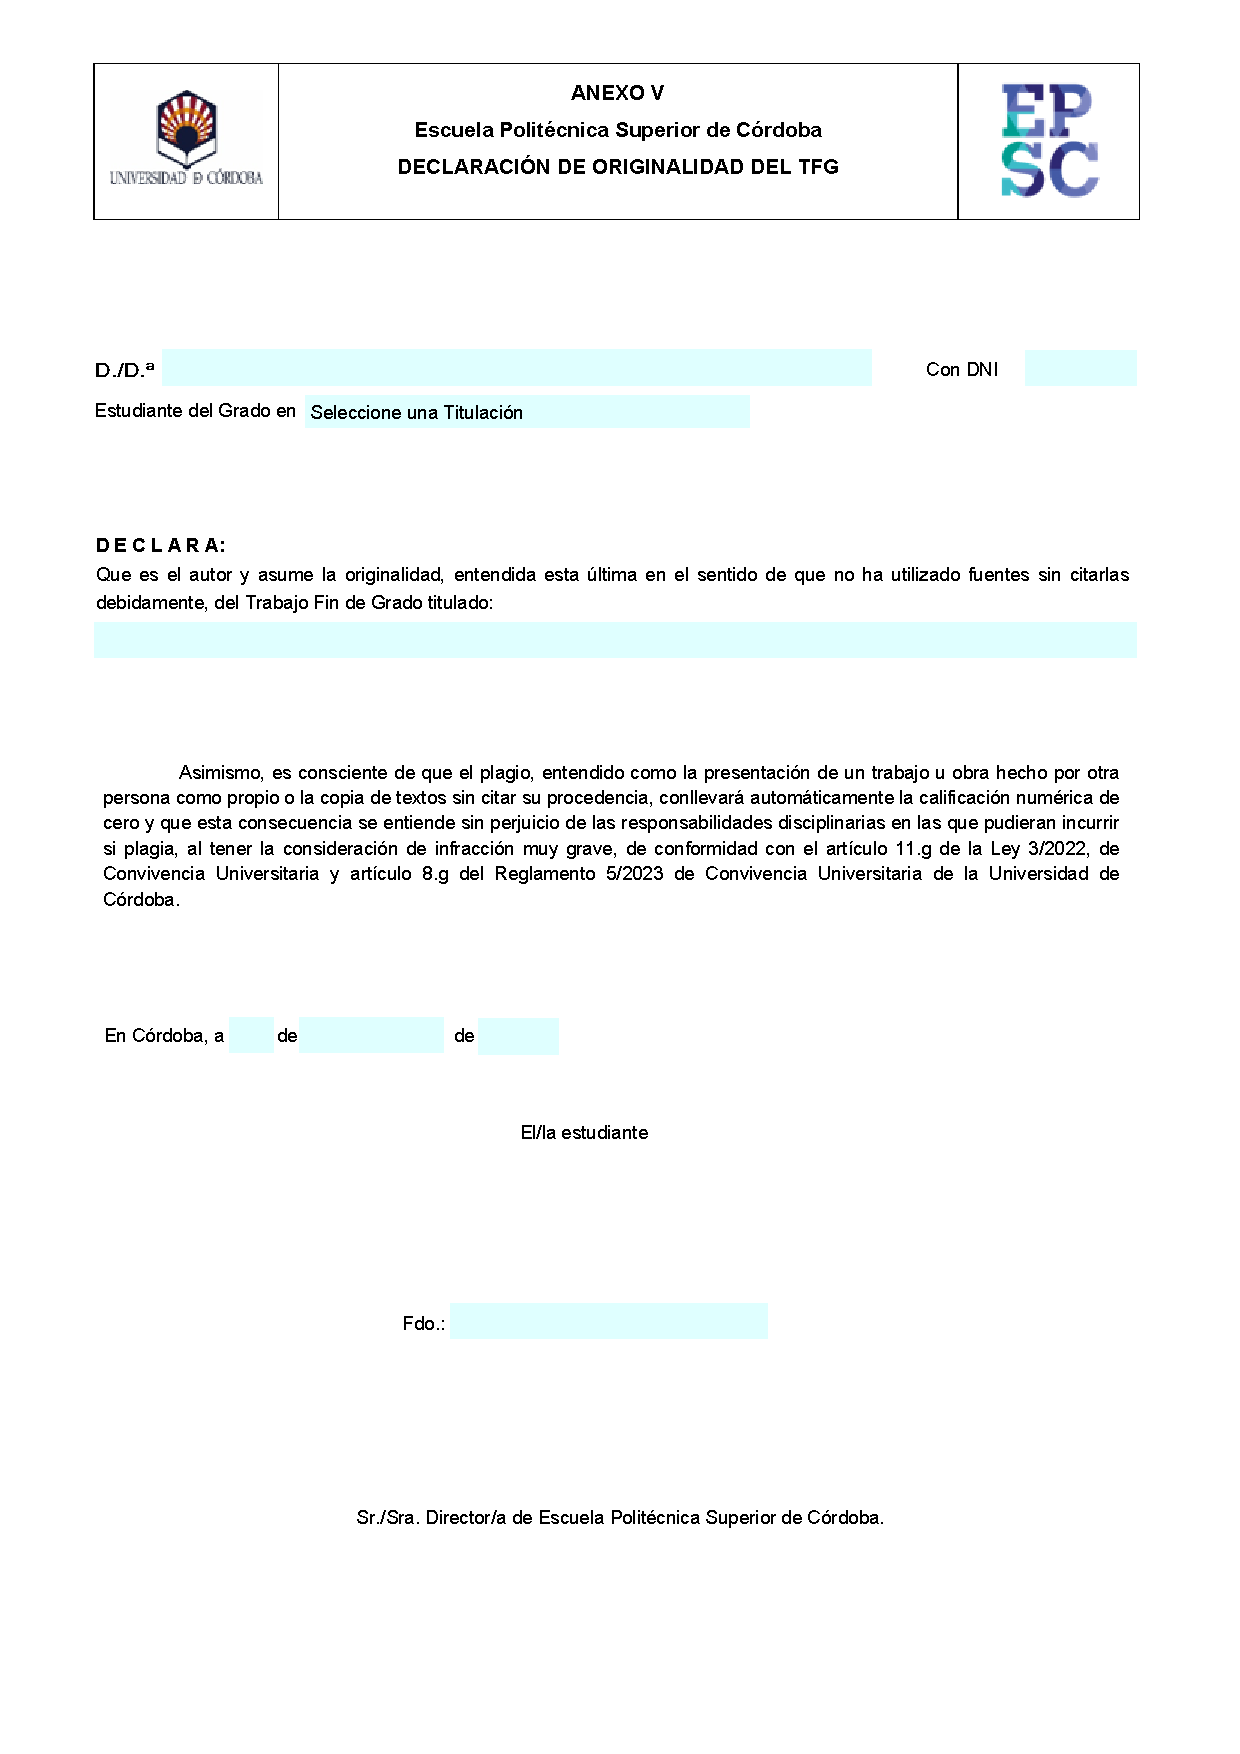
\includepdf[pages=-]{AnexoV/AnexoV_DECLARACION_ORIGINALIDAD_TFG.PDF}

\pagenumbering{Roman} % para comenzar la numeracion de paginas en numeros romanos
\pagestyle{indice}
\thispagestyle{indice}

%%%%%%%%%%%%%%%%%%%
% AGRADECIMIENTOS %
%%%%%%%%%%%%%%%%%%%
\chapter*{Agradecimientos}
\phantomsection
\addcontentsline{toc}{chapter}{Agradecimientos}
\markboth{Agradecimientos}{Agradecimientos}

Este trabajo ha sido posible gracias al acompañamiento académico recibido
durante su desarrollo. Agradezco la orientación del tutor, las observaciones
realizadas durante las revisiones del proyecto y el contexto docente que ha
permitido convertir una idea inicial en una solución funcional, documentada y
evaluada con criterio técnico.

\chapter*{Resumen}
\phantomsection
\addcontentsline{toc}{chapter}{Resumen}
\markboth{Resumen}{Resumen}

\noindent\textbf{Título original:} \TituloTFG

\vspace{0.4cm}

Harmony Hub es una aplicación móvil orientada a transformar el estado
emocional y contextual del usuario en una experiencia musical más útil para su
bienestar cotidiano. La solución combina un check-in guiado, una lógica de
recomendación contextual, un catálogo musical estructurado, la materialización
de playlists reales en Spotify y un ciclo de aprendizaje apoyado en feedback.
Desde el punto de vista técnico, el sistema se construye sobre un cliente móvil
en Flutter, un backend en FastAPI, persistencia documental en Firestore y un
modelo supervisado a nivel de sesión cuya activación solo se permite cuando
existe evidencia objetiva suficiente.

El proceso de recomendación no depende exclusivamente de un modelo de
aprendizaje automático. En su lugar, el sistema adopta un enfoque híbrido: una
capa heurística garantiza operatividad desde la primera sesión, mientras que un
modelo de regresión logística puede reordenar los modos candidatos cuando se
alcanzan mínimos de datos, cobertura por clase y calidad global. El ranking
musical principal se realiza sobre el catálogo propio \texttt{msd\_tracks},
mientras que Spotify se utiliza principalmente para autenticación, lectura de
contexto musical básico y materialización final de la playlist. Esta decisión
permite mantener utilidad incluso bajo restricciones externas, como cambios en
endpoints, limitaciones de cuota o ausencia de datos de entrenamiento
suficientes.

El proyecto explora así cómo combinar software móvil, APIs externas, datos
contextuales y aprendizaje progresivo para acompañar momentos cotidianos de
regulación emocional sin plantearse como una herramienta clínica. En el estado
actual del entregable, el aprendizaje individual del perfil ya es visible en la
experiencia y deja evidencia longitudinal sobre los cinco estados emocionales
considerados. Además, el modelo supervisado de sesión se encuentra activo bajo
puertas explícitas de calidad y puede aportar reordenación probabilística sin
perder la capacidad de abstención cuando la evidencia es débil. La validación
realizada muestra también que la medición del entorno acústico puede integrarse
en el contexto de recomendación y en la generación de playlists. El resultado
es un prototipo funcional que demuestra la viabilidad de una recomendación
musical explicable, orientada a sesiones y capaz de crear playlists reales en
Spotify con trazabilidad contextual y aprendizaje progresivo.

\chapter*{Abstract}
\phantomsection
\addcontentsline{toc}{chapter}{Abstract}
\markboth{Abstract}{Abstract}

Harmony Hub is a mobile application designed to transform a user's emotional and
contextual state into a more useful musical experience for everyday wellbeing.
The system combines a guided check-in, contextual recommendation logic, a
structured music catalogue, Spotify-based playlist materialization and a
feedback-based learning cycle. From a technical point of view, the solution is
built around a Flutter mobile client, a FastAPI backend, document persistence
in Firestore and a supervised session-level model that is only enabled when
there is sufficient objective evidence to justify its use.

The recommendation process does not rely exclusively on a machine learning
model. Instead, it follows a hybrid approach: a heuristic layer guarantees
operability from the first session, while a logistic regression model can later
reorder candidate session modes when enough historical data, class balance and
quality metrics are available. The musical ranking itself is primarily carried
out over the project's own \texttt{msd\_tracks} catalogue, whereas Spotify is
used mainly for authorization, profile context and final playlist
materialization. This design allows the application to remain useful even under
external constraints such as limited Spotify endpoints or insufficient training
data. The result is not merely a musical suggestion, but a real playlist
generated in the user's Spotify account and linked to a traceable session
history.

The project therefore explores how mobile software, external APIs, contextual
data and progressive learning can be combined to support everyday moments of
emotional regulation without positioning the app as a clinical tool. In its
current state, the user-level progressive profile is already operational and
visible in the experience, with longitudinal evidence across the five
emotional states considered in the validation process. The supervised
session-level model is also active under explicit quality gates and can
contribute probabilistic reordering of candidate session modes while still
preserving abstention when evidence is weak. The validation additionally shows
that environmental sensing can be incorporated into both the recommendation
context and the playlist generation pipeline. The outcome is a functional
prototype that demonstrates the viability of a wellness-oriented,
session-based and explainable music recommendation approach with real Spotify
playlist creation, contextual traceability and progressive learning.

\chapter*{Palabras clave}
\phantomsection
\addcontentsline{toc}{chapter}{Palabras clave}
\markboth{Palabras clave}{Palabras clave}

\noindent\textbf{Palabras clave:} bienestar digital, regulación emocional cotidiana, recomendación musical contextual, sistema híbrido de recomendación, playlists adaptativas, aprendizaje progresivo del usuario, aprendizaje supervisado, catálogo musical estructurado, Spotify, Flutter, FastAPI, Firestore.

\chapter*{Key words}
\phantomsection
\addcontentsline{toc}{chapter}{Key words}
\markboth{Key words}{Key words}

\vspace{0.4cm}

\noindent\textbf{Key words:} digital wellbeing, everyday emotional regulation, contextual music recommendation, hybrid recommender system, adaptive playlists, progressive user learning, supervised learning, structured music catalogue, Spotify, Flutter, FastAPI, Firestore.


%%%%%%%%%%%%%%%%%%
% INDICE GENERAL %
%%%%%%%%%%%%%%%%%%
\newpage
\thispagestyle{fancy} 

\phantomsection
\pdfbookmark[0]{Índice general}{indice-general}
\tableofcontents

\cleardoublepage
\phantomsection
\pdfbookmark[0]{Índice de figuras}{indice-figuras}
\listoffigures

\cleardoublepage
\phantomsection
\pdfbookmark[0]{Índice de tablas}{indice-tablas}
\listoftables

% Índice de diagramas de flujo. Descomenta este bloque si usas el entorno "diagrama".
% \cleardoublepage
% \phantomsection
% \addcontentsline{toc}{chapter}{Índice de diagramas de flujo}
% \listofdiagrams

% Lista de acrónimos.
\phantomsection
\pdfbookmark[0]{Lista de acrónimos}{lista-acronimos}
\addcontentsline{toc}{chapter}{Lista de Acrónimos}
\glsaddall[types=\acronymtype]
\printnoidxglossary[type=\acronymtype, title={Lista de Acrónimos}, nonumberlist]
\clearpage

%---------------------%
%	CUERPO DE TEXTO   %
%---------------------%

\pagestyle{cuerpo}
\thispagestyle{cuerpo}

\pagenumbering{arabic}

%%%%%%%%%%%%%%%%%%%%%%%%%%%%%%%%%%%%%%%%%%%%%%%%%%%%%%%%%%%%%%%%%%%%%
%                         ESTRUCTURA CONTENIDO                      %
%%%%%%%%%%%%%%%%%%%%%%%%%%%%%%%%%%%%%%%%%%%%%%%%%%%%%%%%%%%%%%%%%%%%%

% Estructura principal preparada para un TFG de tipo:
% b) Análisis y resolución de casos prácticos reales en el ámbito de la ingeniería.
% Si tu TFG pertenece a otra tipología, revisa el archivo GUIA_RELLENO.md y adapta
% los capítulos indicados.

%------------------%
%     CAPÍTULOS    %
%------------------%

\chapter{Introducción y contexto}
\label{ch:introduccion}

\section{Contexto general}
\label{sec:contexto_general}

En los últimos años se ha vuelto cada vez más evidente que el bienestar cotidiano no depende solo de grandes decisiones, sino también de pequeños mecanismos de autorregulación que usamos casi sin darnos cuenta para sobrellevar el día. La carga mental, la sobreexposición a estímulos, el ruido ambiental y la sensación de ir siempre con prisa forman parte de la rutina de muchas personas, especialmente en entornos urbanos y digitales. De hecho, la Organización Mundial de la Salud ha señalado que el ruido ambiental constituye un problema relevante de salud pública y que su impacto afecta al descanso, al rendimiento y al bienestar general \cite{who_noise_2018}.

En medio de ese contexto, la música ocupa un papel relevante. No suele vivirse únicamente como entretenimiento: con frecuencia funciona como refugio, como impulso o como una forma de recuperar equilibrio. Además, distintos trabajos han mostrado que las prácticas artísticas pueden desempeñar un papel valioso en la promoción de la salud y el bienestar, mientras que estudios centrados en el uso de la música en contextos reales apuntan a que las personas la emplean para modular estados emocionales concretos \cite{who_arts_2019,thoma2012}.

Sin embargo, existe una distancia clara entre ese potencial y la forma en la que las plataformas musicales más extendidas acompañan realmente al usuario. La mayoría de estos servicios están diseñados para recomendar canciones en función del historial de escucha, la popularidad o la permanencia dentro de la plataforma. Ese enfoque resulta útil para descubrir música o mantener el consumo, pero no siempre responde a una necesidad funcional concreta: qué escuchar cuando una persona necesita concentrarse, rebajar la tensión, sentirse acompañada o recuperar energía sin dedicar tiempo adicional a decidirlo.

En ese cruce entre necesidad cotidiana, tecnología móvil y personalización musical se sitúa Harmony Hub. El proyecto parte de una idea sencilla, aunque ambiciosa: utilizar la interacción breve con una aplicación móvil para captar el momento actual del usuario y transformar esa información en una propuesta musical con intención, conectada además con una plataforma real de reproducción como Spotify.

\section{Motivación}
\label{sec:motivacion}

La motivación de este trabajo nace de una observación frecuente: muchas personas ya usan la música para regularse, pero lo hacen de forma manual, improvisada y, en ocasiones, poco eficaz. Abrir una aplicación, saltar entre listas, probar varias canciones y confiar en que alguna encaje con el estado de ánimo del momento es una rutina habitual. Aunque la oferta musical disponible es inmensa, esa abundancia no siempre se traduce en claridad.

Desde esa perspectiva, Harmony Hub surge como una propuesta orientada a acompañar mejor ese gesto cotidiano. No pretende convertir la música en una solución mágica ni ocupar el lugar de herramientas clínicas o terapéuticas. Lo que busca, más bien, es ofrecer una experiencia digital capaz de traducir señales sencillas del usuario ---como su estado de ánimo, nivel de energía, estrés percibido o intención de la sesión--- en una recomendación musical más coherente con su situación real.

Además, el proyecto posee un interés académico y técnico claro dentro del ámbito de la Ingeniería Informática. Reúne desarrollo móvil, backend, persistencia de datos, integración con APIs externas, diseño de interacción y una capa de aprendizaje basada en feedback. Esa combinación permite abordar un caso práctico donde la tecnología no se plantea solo como infraestructura, sino como medio para construir una experiencia contextual y mejor adaptada a necesidades de bienestar.

\section{Problema que se aborda}
\label{sec:problema_abordado}

El problema central que aborda este TFG puede formularse de la siguiente manera: las plataformas musicales generalistas ofrecen acceso masivo a contenido y sistemas sofisticados de recomendación, pero no están pensadas, al menos de forma principal, para ayudar al usuario a alcanzar un estado funcional o emocional concreto en un momento determinado y, además, aprender del uso para mejorar progresivamente la interacción.

Esta limitación se percibe con especial claridad en situaciones cotidianas como empezar una sesión de estudio, bajar revoluciones después de un día exigente, combatir la fatiga mental o buscar una sensación de compañía emocional. En esos casos, el usuario no necesita solo ``música que le guste'', sino música que encaje con un contexto, una necesidad y una intención. La diferencia es sutil, pero importante: no se trata únicamente de afinidad musical, sino de pertinencia situacional.

Además, muchas soluciones existentes dejan fuera parte del ciclo completo. Algunas permiten descubrir canciones; otras facilitan organizar playlists; otras registran hábitos o estados personales. Sin embargo, resulta menos habitual encontrar una herramienta que conecte, de forma fluida, los siguientes elementos dentro de una misma experiencia: un check-in breve, una interpretación contextual del momento, una generación de playlist reproducible en una plataforma real y, finalmente, una recogida de feedback que permita aprender de lo que ha funcionado y de lo que no.

Por tanto, el problema no es la falta de música ni la falta de algoritmos de recomendación, sino la ausencia de una capa intermedia capaz de convertir el momento personal del usuario en una propuesta musical útil, comprensible y progresivamente más afinada.

\section{Alcance del trabajo}
\label{sec:alcance}

El alcance de este trabajo se centra en el análisis, diseño y desarrollo de una solución funcional que materializa esa idea en forma de plataforma móvil. Harmony Hub permite al usuario registrarse, realizar un check-in emocional y contextual, obtener una recomendación de sesión, generar una playlist asociada dentro de Spotify, consultar el historial de uso y aportar feedback para alimentar el aprendizaje posterior del sistema.

Desde el punto de vista técnico, el proyecto incluye una aplicación móvil desarrollada con Flutter, un backend construido con FastAPI, persistencia en servicios asociados a Firebase/Firestore e integración con la API de Spotify. Además, incorpora una capa de personalización basada en reglas, contexto y feedback histórico del usuario, así como un catálogo musical estructurado propio, \texttt{msd\_tracks}, sobre el que se apoya la selección principal de canciones. La integración con Spotify se reserva sobre todo para la autenticación, el acceso al perfil musical básico y la materialización final de playlists reproducibles. A ello se suma un modelo de aprendizaje supervisado a nivel de sesión que solo se activa cuando existe evidencia suficiente para justificar su uso. En la versión actual del sistema conviven, por tanto, dos ritmos de adaptación: un aprendizaje individual progresivo del perfil musical del usuario, ya operativo y visible en la experiencia, y un clasificador supervisado global que solo interviene cuando supera puertas objetivas de datos y calidad y, además, alcanza confianza suficiente en la sesión concreta.

En coherencia con ese enfoque, la validación experimental del aprendizaje se plantea sobre un único perfil longitudinal de usuario. Esta decisión no reduce el alcance funcional de la plataforma, que sigue siendo multiusuario, pero sí simplifica la interpretación de la adaptación progresiva del sistema y facilita explicar con mayor claridad cuándo aprende, cuándo se abstiene y por qué. La evidencia disponible distingue dos planos: un perfil musical individual ya afinado por el uso acumulado y un modelo supervisado global que ya puede intervenir cuando supera sus puertas de calidad y confianza en el contexto de sesión evaluado.

En términos de evidencia disponible, esa validación longitudinal ya no se apoya
en unas pocas sesiones aisladas, sino en un conjunto supervisado que ha
alcanzado 66 ejemplos etiquetados, con cobertura completa de los cinco estados
emocionales principales trabajados en la aplicación. Sobre esa base, el
proyecto no se limita a mostrar aprendizaje individual visible, sino que activa
también el clasificador supervisado global bajo puertas explícitas de calidad y
un umbral operativo de confianza. Esta situación refuerza el interés académico
del proyecto porque permite observar, dentro de una misma arquitectura, tres
niveles de comportamiento diferenciados: recomendación heurística trazable,
aprendizaje individual progresivo y participación real del componente
supervisado cuando existe evidencia suficiente para ello.

Conviene subrayar también los límites del proyecto. Harmony Hub no se plantea como dispositivo médico, herramienta diagnóstica ni sustituto de apoyo psicológico profesional. Tampoco persigue resolver la recomendación musical de forma universal ni competir con motores comerciales de gran escala. Su propósito es más acotado y, a la vez, más concreto: explorar cómo una aplicación móvil puede acompañar mejor momentos cotidianos de regulación emocional y bienestar a través de playlists adaptativas y una interacción breve, comprensible y usable.

\section{Estructura de la memoria}
\label{sec:estructura_memoria}

La memoria se organiza como un recorrido progresivo que va desde el problema de partida hasta la validación del sistema implementado. Esta estructura pretende facilitar una lectura acumulativa: primero se justifica por qué resulta pertinente construir Harmony Hub, después se define qué debe resolver, a continuación se explica cómo se diseña y desarrolla la solución, y finalmente se contrasta qué resultados ofrece y cuáles son sus límites.

En el Capítulo~\ref{ch:objetivos} se formulan el objetivo general y los objetivos específicos que orientan el trabajo. El Capítulo~\ref{ch:antecedentes} sitúa la propuesta dentro del contexto de las plataformas musicales, las aplicaciones orientadas al bienestar y los sistemas de personalización basados en datos, con el fin de delimitar el hueco funcional que Harmony Hub busca cubrir.

El Capítulo~\ref{ch:analisis_problema} recoge el análisis del problema, la especificación de requisitos, la descripción de la información manejada y los casos de uso principales. Sobre esa base, el Capítulo~\ref{ch:diseno_solucion} presenta el diseño lógico y arquitectónico del sistema, incluyendo sus diagramas, el flujo principal de generación de sesión musical y la organización de los componentes que sostienen la recomendación y el aprendizaje.

El Capítulo~\ref{ch:desarrollo_implementacion} describe la materialización técnica del proyecto en Flutter, FastAPI, Firestore y Spotify, así como las decisiones adoptadas en persistencia, seguridad, privacidad y modelado del aprendizaje. El Capítulo~\ref{ch:pruebas_validacion} expone las pruebas realizadas, la evidencia verificada y la discusión de los resultados obtenidos a partir de la validación funcional, técnica y longitudinal del sistema.

Por su parte, el Capítulo~\ref{ch:planificacion_recursos} resume la organización temporal del proyecto, sus fases de desarrollo, las desviaciones introducidas durante la ejecución y los recursos finalmente empleados. El Capítulo~\ref{ch:conclusiones} cierra la memoria con una síntesis del trabajo realizado, sus principales aportaciones y las líneas de evolución que resultan más justificadas a partir del estado final alcanzado.

La memoria se completa con varios anexos de carácter técnico y práctico. Estos materiales complementarios permiten documentar con mayor detalle cuestiones de uso, implementación y apoyo al análisis sin sobrecargar la lectura principal del documento.

\chapter{Objetivos}
\label{ch:objetivos}

% Deben coincidir con los objetivos aprobados en la solicitud/anteproyecto del TFG.

\section{Objetivo general}
\label{sec:objetivo_general}

El objetivo general de este Trabajo Fin de Grado es analizar, diseñar y desarrollar una plataforma móvil inteligente que ayude al usuario a convertir su estado emocional y contextual del momento en una experiencia musical más útil para su bienestar cotidiano, mediante recomendaciones de sesión, un catálogo musical estructurado y playlists adaptativas materializadas en Spotify.

De forma más concreta, se persigue construir una solución funcional que no se limite a recomendar música por afinidad histórica, sino que sea capaz de interpretar el momento presente del usuario, acompañarlo con una propuesta musical coherente y aprender progresivamente a partir del uso y del feedback recibido.

\section{Objetivos específicos}
\label{sec:objetivos_especificos}

\begin{enumerate}[label=OE\arabic*.]
    \item Analizar el problema de la regulación cotidiana mediante música en entornos digitales y definir los requisitos funcionales y no funcionales que debe cumplir una solución centrada en este caso de uso.
    \item Diseñar una arquitectura software compuesta por aplicación móvil, backend e integración con servicios externos que permita sostener de forma clara y escalable el flujo completo del sistema.
    \item Implementar una aplicación móvil usable que permita al usuario registrarse, autenticarse, realizar un check-in breve, consultar su historial y navegar por la experiencia sin fricción innecesaria.
    \item Desarrollar un mecanismo de recomendación de sesión capaz de transformar variables como el estado de ánimo, la energía, el estrés percibido o la intención del usuario en una propuesta musical contextualizada, explicable y apoyada en un catálogo propio.
    \item Integrar la plataforma con Spotify para que las recomendaciones generadas puedan materializarse en playlists reales, reproducibles y asociadas a la cuenta del usuario sin delegar en la API externa la fase central de ranking musical.
    \item Incorporar un ciclo de aprendizaje basado en feedback, persistencia de datos e indicadores objetivos que permita afinar progresivamente la personalización en dos niveles: un aprendizaje individual del perfil del usuario, visible en la experiencia, y un modelo supervisado a nivel de sesión cuya activación quede condicionada por puertas explícitas de datos, calidad global y confianza operativa en la sesión concreta.
    \item Validar la solución construida mediante pruebas funcionales, revisión de flujos completos de uso y métricas objetivas en los componentes de aprendizaje, con el fin de comprobar que el sistema responde de forma coherente a los objetivos planteados.
\end{enumerate}

\section{Relación entre objetivos y resultados esperados}
\label{sec:objetivos_resultados}

El cumplimiento de los objetivos anteriores no se evaluará solo desde una perspectiva descriptiva, sino a través de resultados observables dentro del sistema desarrollado. Esto permite conectar cada objetivo con una evidencia concreta y, además, preparar mejor la validación posterior del proyecto.

\begin{table}[H]
\centering
\begin{tabular}{|p{1.6cm}|p{6cm}|p{6cm}|}
\hline
\textbf{Objetivo} & \textbf{Resultado esperado} & \textbf{Evidencia de cumplimiento} \\
\hline
OE1 & Definición clara del problema, de los actores implicados y de los requisitos del sistema. & Capítulo~\ref{ch:analisis_problema}, con requisitos funcionales, no funcionales, casos de uso y restricciones. \\
\hline
OE2 & Propuesta arquitectónica coherente para articular frontend, backend, datos e integraciones externas. & Capítulo~\ref{ch:diseno_solucion}, con la arquitectura general, diseño funcional y decisiones técnicas justificadas. \\
\hline
OE3 & Aplicación móvil operativa con flujos de acceso, check-in, navegación principal, historial y perfil. & Capítulo~\ref{ch:desarrollo_implementacion}, demostración de pantallas implementadas y pruebas funcionales del flujo de uso. \\
\hline
OE4 & Generación de recomendaciones de sesión a partir del contexto declarado por el usuario. & Implementación del flujo check-in $\rightarrow$ recomendación y validación del comportamiento del sistema en el Capítulo~\ref{ch:pruebas_validacion}. \\
\hline
OE5 & Creación de playlists reales dentro de Spotify a partir de la recomendación generada. & Integración backend--Spotify, resolución de canciones desde el catálogo propio y comprobación del flujo completo desde la app hasta la cuenta del usuario. \\
\hline
OE6 & Persistencia del historial, recogida de feedback y activación controlada de aprendizaje progresivo. & Registro de sesiones y feedback, almacenamiento en base de datos, señales observables del aprendizaje individual del perfil y métricas objetivas del modelo de sesión, incluyendo puertas de calidad globales y específicas por mood. \\
\hline
OE7 & Evidencia de que la solución responde de forma estable a los objetivos del TFG. & Pruebas funcionales, revisión de incidencias corregidas, validación del flujo completo y análisis de métricas del sistema en el Capítulo~\ref{ch:pruebas_validacion}. \\
\hline
\end{tabular}
\caption{Relación entre los objetivos específicos y los resultados esperados del proyecto.}
\label{tab:objetivos_resultados}
\end{table}

De este modo, cada objetivo queda vinculado a una salida concreta del proyecto: análisis, arquitectura, implementación, integración, aprendizaje o validación. Ésta trazabilidad resulta especialmente útil en un trabajo como Harmony Hub, donde la calidad de la propuesta no depende solo de que la aplicación exista, sino de que el conjunto de piezas funcione como una experiencia coherente y justificable.

\chapter{Antecedentes y soluciones existentes}
\label{ch:antecedentes}

% Este capítulo cubre el apartado "Antecedentes" de la guía: análisis comparativo
% de soluciones existentes y relación con los objetivos del proyecto.

\section{Situación actual}
\label{sec:situacion_actual}

En la práctica, el problema que aborda Harmony Hub se resuelve hoy de forma fragmentada. Cuando una persona quiere usar la música para concentrarse, bajar el nivel de activación, sentirse acompañada o simplemente atravesar mejor un momento concreto del día, suele recurrir a tres caminos habituales.

El primero consiste en apoyarse en plataformas generalistas de streaming musical, como Spotify, que ofrecen listas personalizadas generadas algorítmicamente a partir del historial de escucha, los temas que se guardan, el momento de uso y los patrones de usuarios con gustos similares \cite{spotify_playlists}. Este enfoque funciona muy bien para descubrimiento y afinidad musical, pero su lógica principal sigue estando ligada a los hábitos de consumo y no a una lectura explícita del estado emocional o de la necesidad puntual del usuario.

El segundo camino se encuentra en aplicaciones de bienestar digital orientadas a foco, relajación o sueño. Herramientas como Endel, Brain.fm o Headspace proponen experiencias sonoras o musicales para ayudar a entrar en ciertos estados de atención, descanso o calma \cite{endel_technology,brainfm_official,headspace_focus}. Aquí el acento ya no está tanto en ``qué música te gusta'', sino en ``qué estado quieres favorecer''. Ese enfoque las aproxima al problema que aborda Harmony Hub.

Sin embargo, la situación actual deja un hueco interesante. Por un lado, las plataformas de streaming tienen un catálogo inmenso y una integración natural con la escucha real del usuario, pero no suelen empezar con un check-in emocional breve ni cerrar el ciclo con una recogida estructurada de feedback sobre la utilidad de la sesión. Por otro, las aplicaciones de bienestar suelen ofrecer audio funcional o contenido guiado, aunque normalmente dentro de ecosistemas cerrados, con menor relación con la biblioteca musical cotidiana del usuario o con sus cuentas de streaming. Esta lectura comparativa es una inferencia a partir de las funcionalidades públicas revisadas en cada solución.

Por tanto, el contexto actual no muestra una ausencia de herramientas, sino más bien una dispersión de enfoques. Existen soluciones potentes para descubrir música, para mejorar el descanso, para facilitar el foco o para construir rutinas de bienestar. Lo que resulta menos frecuente es encontrar una propuesta que una, en una misma experiencia, bienestar cotidiano, contexto inmediato, personalización musical reproducible y aprendizaje progresivo a partir del uso.

\section{Soluciones relacionadas}
\label{sec:soluciones_relacionadas}

Entre las soluciones más relacionadas con Harmony Hub pueden señalarse cuatro referencias especialmente útiles para entender el espacio de diseño del proyecto.

\textbf{Spotify}. Spotify representa el referente más claro en personalización musical a gran escala. Según su propia documentación, sus playlists personalizadas se construyen con algoritmos que consideran qué escucha la persona, cuándo lo escucha, qué canciones guarda y qué patrones presentan usuarios con gustos parecidos \cite{spotify_playlists}. Además, la compañía subraya que su personalización busca ofrecer el contenido adecuado en el momento adecuado, combinando señales algorítmicas y criterio editorial \cite{spotify_responsible_recs}. Su principal fortaleza es, por tanto, la afinidad musical y la capacidad de descubrimiento. No obstante,  su enfoque no se encuentra centrado en un check-in explícito de bienestar o regulación emocional, sino en la evolución del gusto y del comportamiento de escucha. Esta última idea es una inferencia razonable a partir de la forma en que Spotify presenta sus sistemas de personalización.

\textbf{Endel}. Endel se sitúa en un terreno distinto: no trabaja tanto con canciones concretas como con soundscapes adaptativos. Su tecnología declara usar entradas del usuario y del entorno, como la hora del día, el tiempo, el movimiento o determinados sensores, para generar sonido personalizado en tiempo real orientado a foco, relajación o sueño \cite{endel_technology}. Esta propuesta resulta muy valiosa porque introduce contexto y adaptación dinámica, dos dimensiones especialmente relevantes para Harmony Hub. Aun así, la salida del sistema no es una playlist musical integrada en un servicio de streaming, sino un entorno sonoro funcional propio.

\textbf{Brain.fm}. Brain.fm presenta una propuesta centrada en música diseñada específicamente para favorecer estados como foco, relajación, sueño o meditación. La plataforma enfatiza su orientación científica, el uso de sesiones pensadas para tareas concretas y la idea de ofrecer flujos musicales sin necesidad de búsqueda manual \cite{brainfm_official}. Su valor diferencial está en la intencionalidad del audio y en su promesa de reducir distracciones. Sin embargo, la experiencia sigue articulándose sobre un catálogo y una lógica propios, no sobre playlists generadas en la cuenta musical habitual del usuario ni sobre una lectura contextual rica de su momento cotidiano.

\textbf{Headspace}. Aunque Headspace nace en el ámbito de la meditación y el mindfulness, su ecosistema incluye música para concentración, sueño y relajación, además de ejercicios breves y contenidos guiados \cite{headspace_focus}. En ese sentido, aporta una visión muy sólida del bienestar digital como experiencia acompañada, amable y accesible. Su fortaleza está en la estructura de hábitos, el tono de acompañamiento y la variedad de recursos. No obstante, su núcleo no es la recomendación musical contextual basada en una integración con plataformas como Spotify, sino un entorno propio orientado a meditación, descanso y regulación general.

\begin{figure}[htbp]
\centering
\begin{subfigure}[t]{0.24\textwidth}
    \centering
    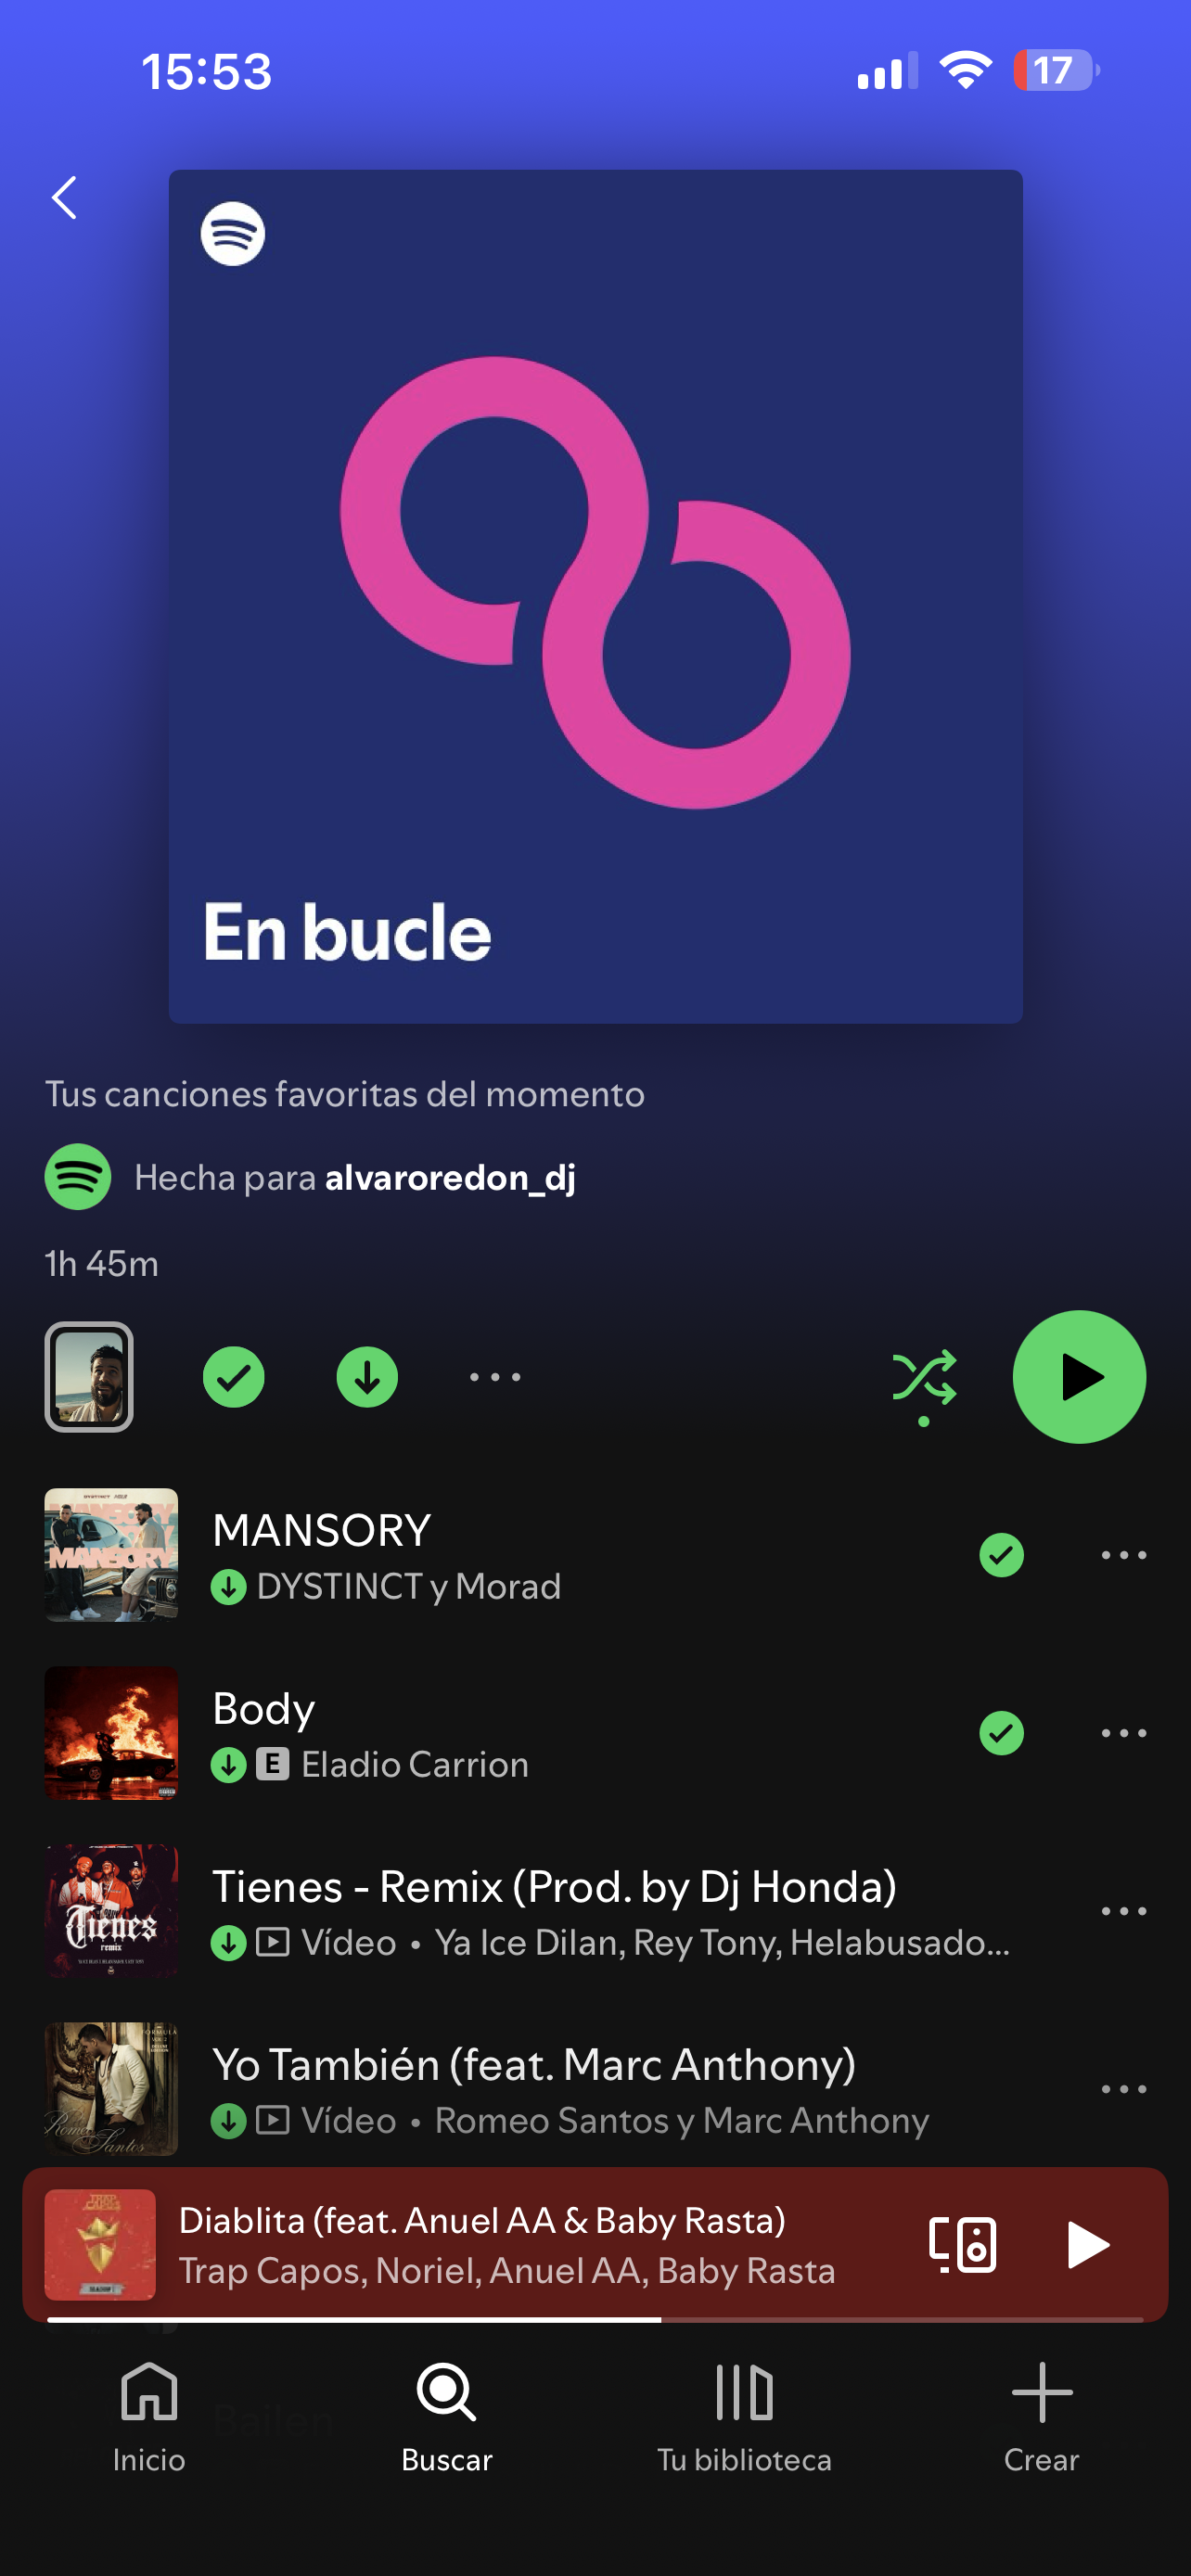
\includegraphics[width=\linewidth]{Imagenes/spotify.PNG}
    \caption{Spotify}
\end{subfigure}
\hfill
\begin{subfigure}[t]{0.24\textwidth}
    \centering
    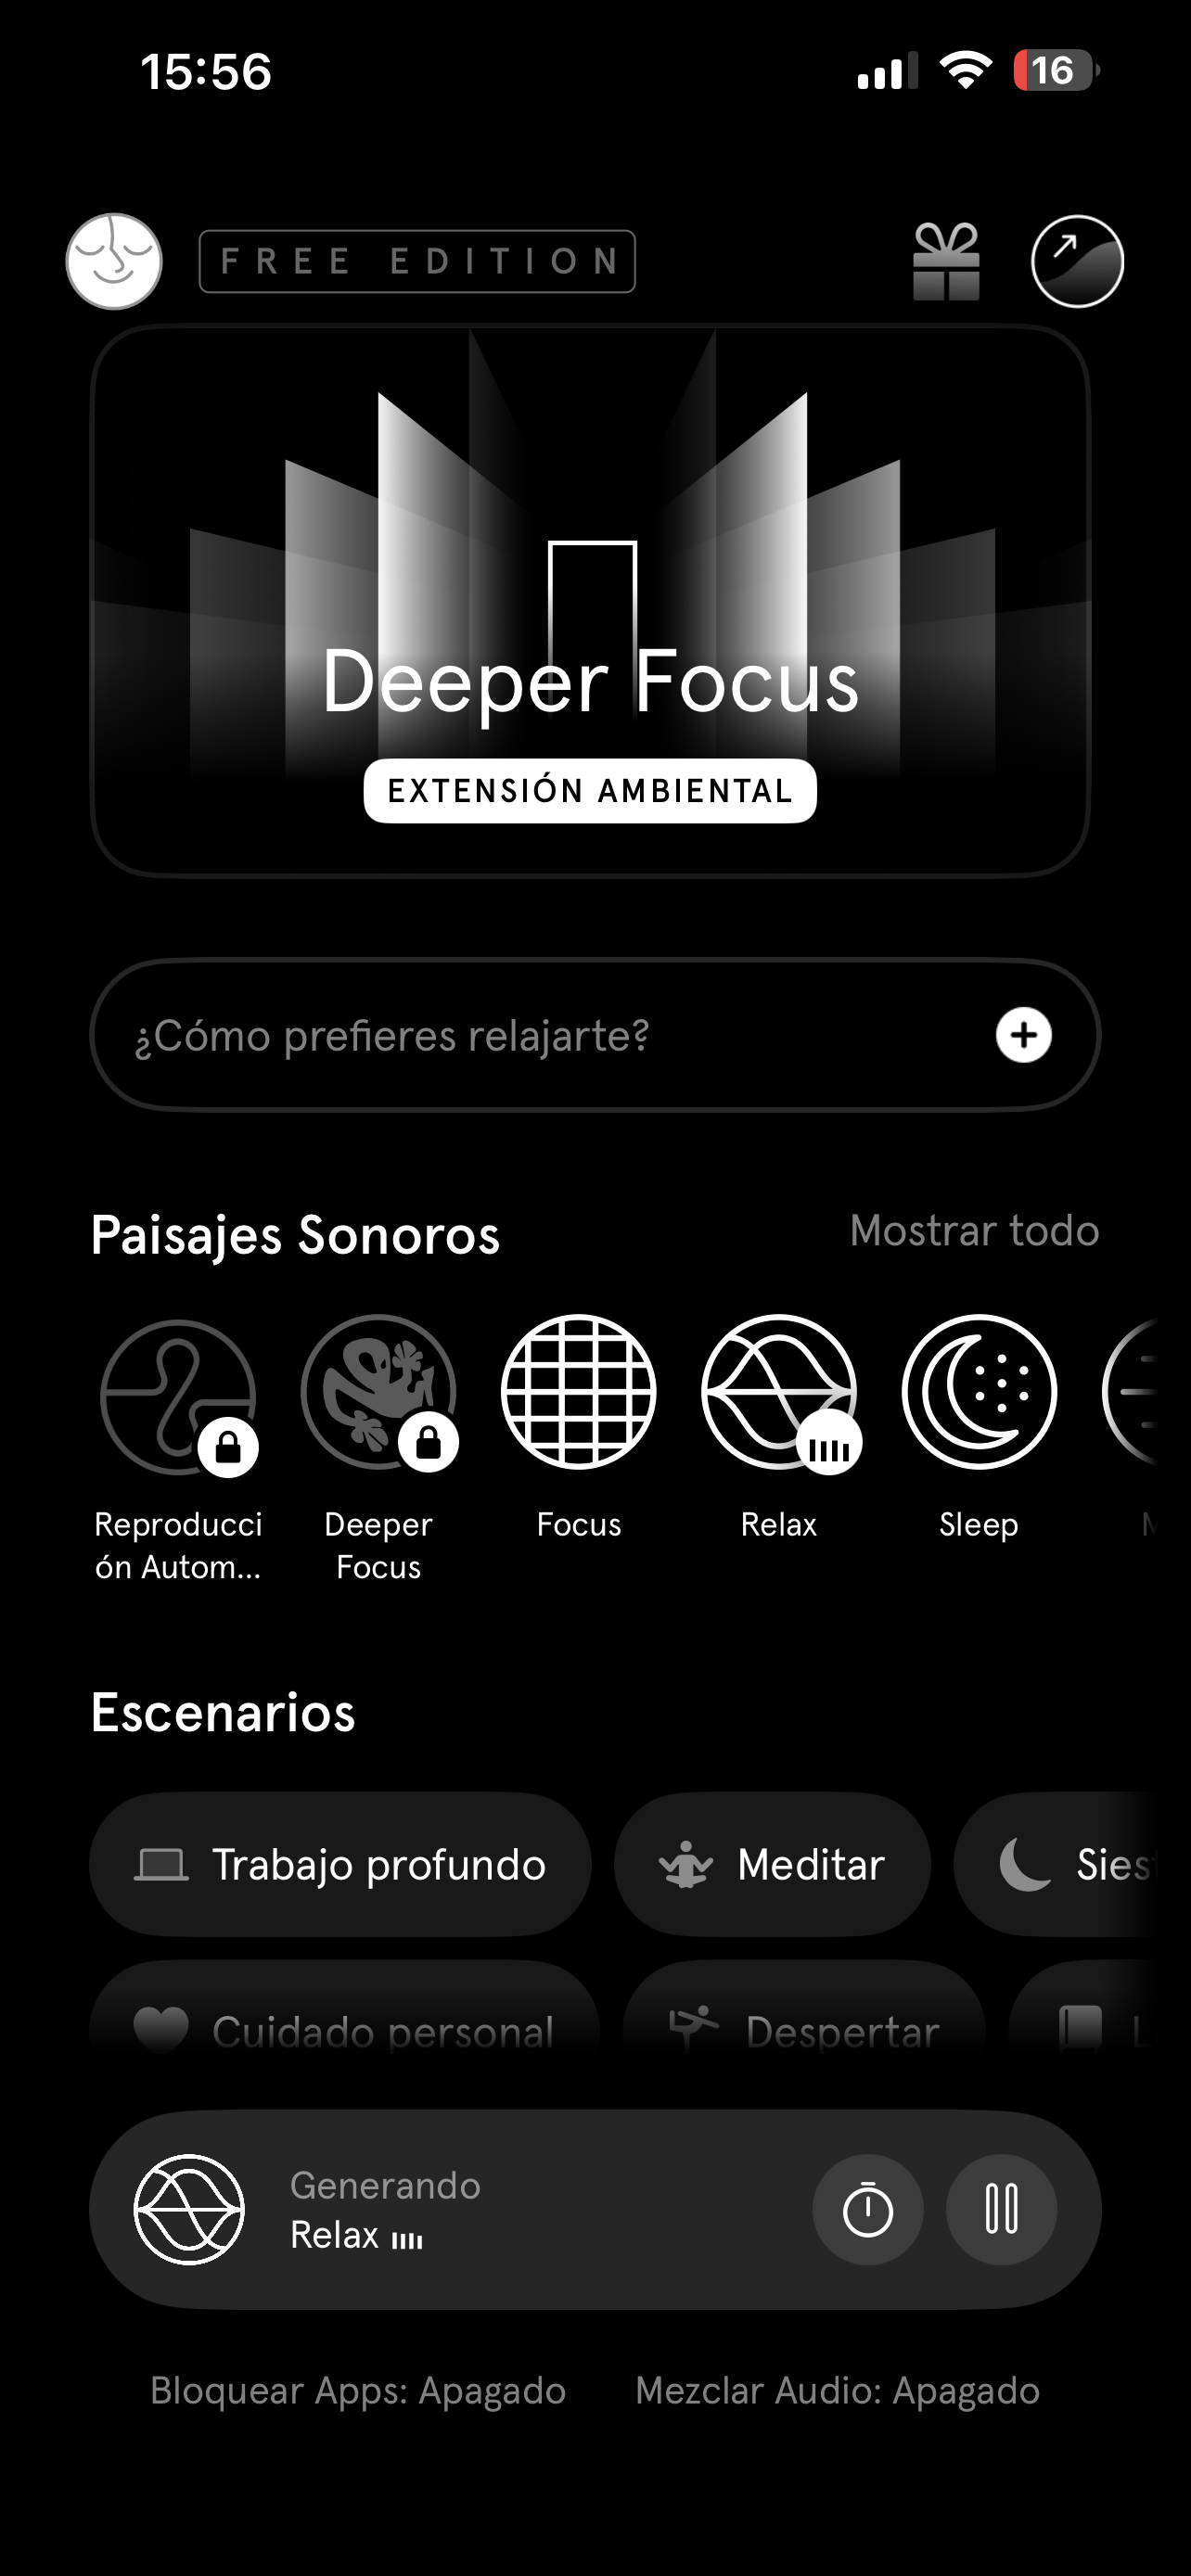
\includegraphics[width=\linewidth]{Imagenes/endel.PNG}
    \caption{Endel}
\end{subfigure}
\hfill
\begin{subfigure}[t]{0.24\textwidth}
    \centering
    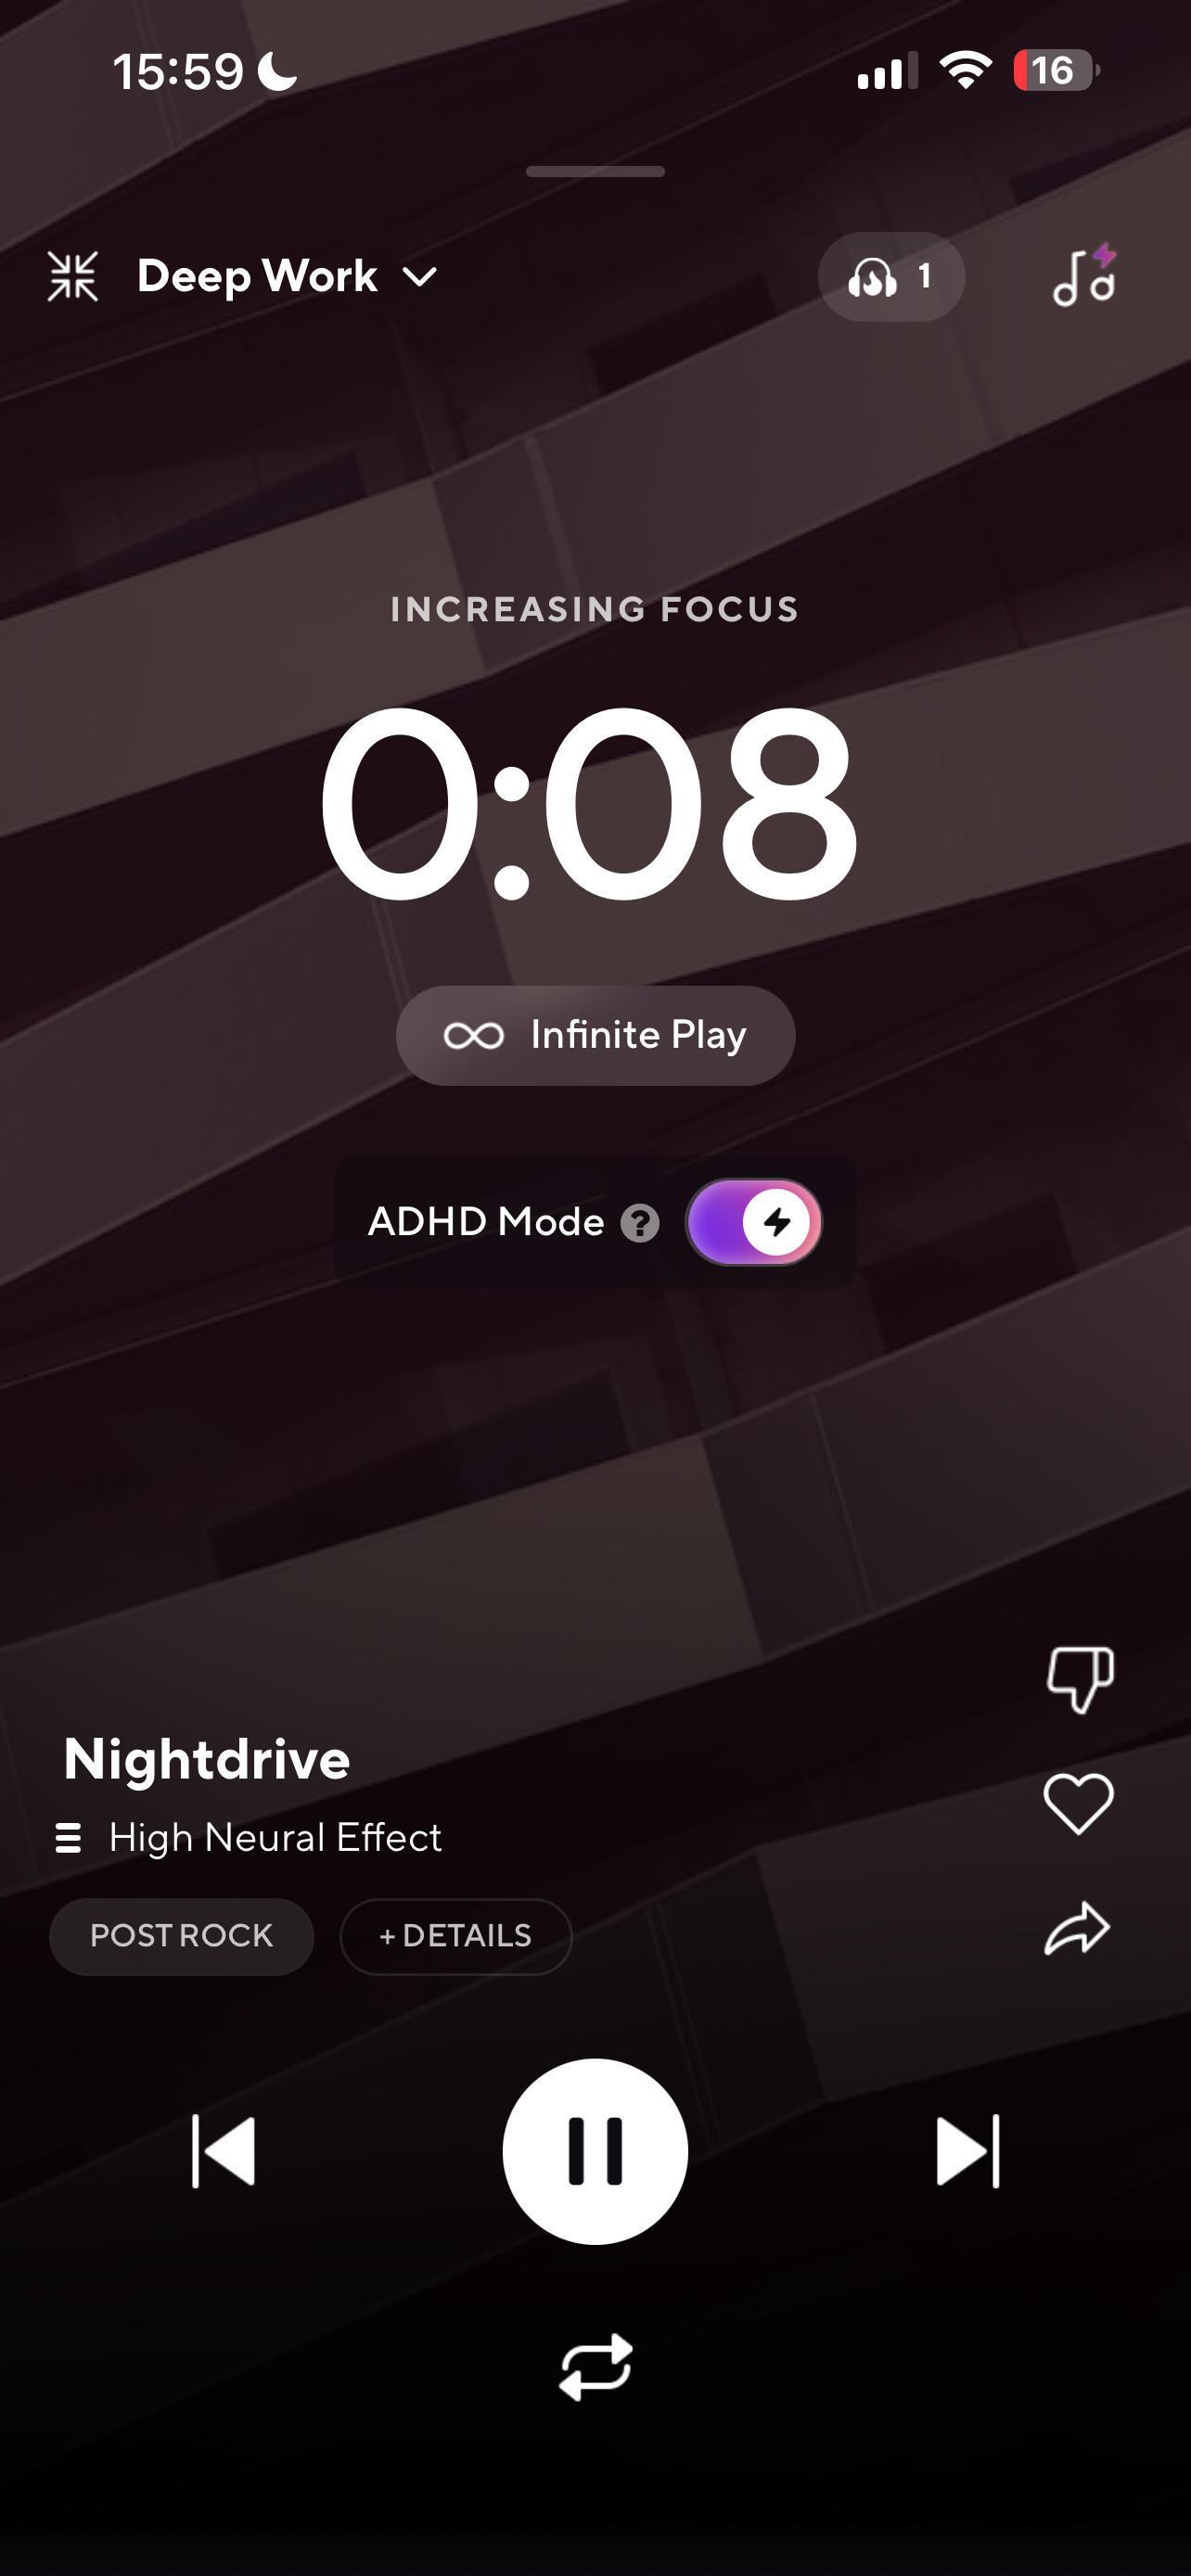
\includegraphics[width=\linewidth]{Imagenes/brainfm.PNG}
    \caption{Brain.fm}
\end{subfigure}
\hfill
\begin{subfigure}[t]{0.24\textwidth}
    \centering
    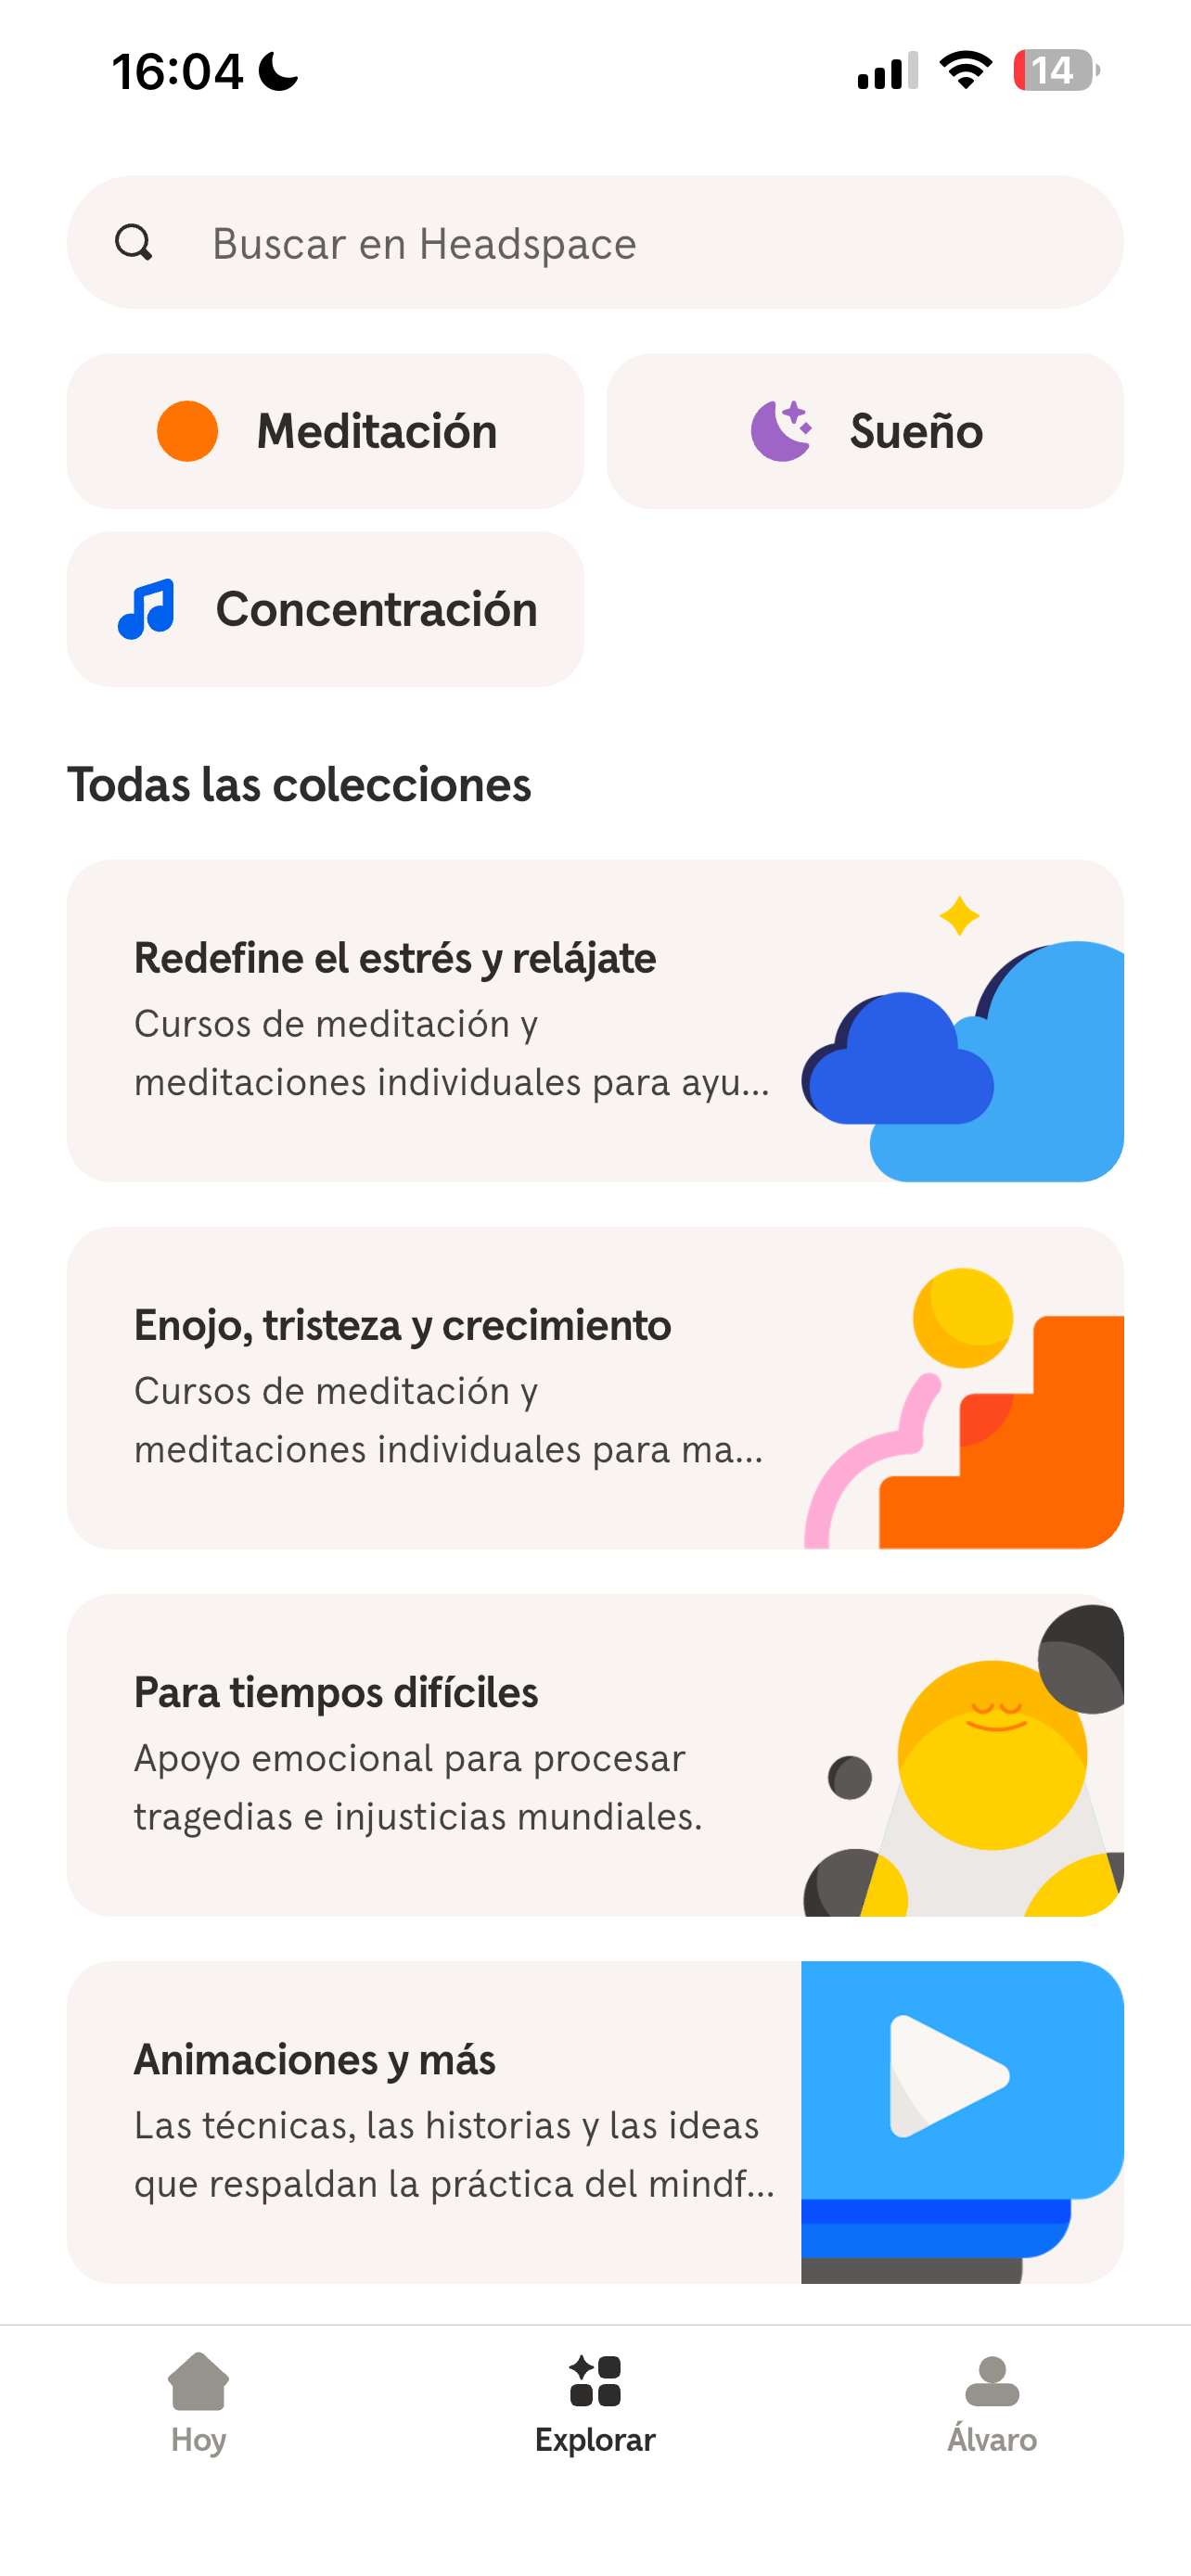
\includegraphics[width=\linewidth]{Imagenes/headspace.PNG}
    \caption{Headspace}
\end{subfigure}
\caption{Capturas representativas de soluciones relacionadas analizadas. Spotify destaca por la playlist personalizada; Endel por el paisaje sonoro adaptativo; Brain.fm por la sesión funcional orientada a foco; y Headspace por el ecosistema de bienestar con secciones de meditación, sueño y concentración.}
\label{fig:apps_relacionadas}
\end{figure}

La figura \ref{fig:apps_relacionadas} ayuda a aterrizar visualmente la comparación anterior. Spotify presenta una interfaz centrada en listas personalizadas y consumo musical habitual; Endel y Brain.fm muestran propuestas donde el audio se articula como sesión funcional o paisaje sonoro; y Headspace organiza la experiencia alrededor de categorías de bienestar como meditación, sueño o concentración. Esta lectura visual refuerza la idea de que Harmony Hub no replica ninguna de estas soluciones de forma directa, sino que toma elementos de varias de ellas para combinarlos en un flujo único con check-in, recomendación contextual, playlist real y feedback.

Vistas en conjunto, estas soluciones muestran que el problema que plantea Harmony Hub no parte de cero. Al contrario: se sitúa en un territorio donde ya existen muy buenas respuestas parciales. Spotify sobresale en personalización musical, Endel en adaptación contextual sonora, Brain.fm en audio funcional orientado a estados concretos y Headspace en experiencia de bienestar guiada. Precisamente por eso, la aportación del proyecto no consiste en negar esas referencias, sino en dialogar con ellas y proponer una combinación diferente favoreciendo al usuario en su bienestar personal.

\section{Evidencia sobre música y bienestar psicológico}
\label{sec:evidencia_musica_bienestar}

Además de las soluciones comerciales analizadas, existe una base académica que
justifica la relación entre música, bienestar y regulación psicológica. La
revisión de alcance de la OMS sobre artes y salud concluye que las actividades
artísticas, incluidas distintas formas de participación musical, pueden
contribuir a reducir malestar psicológico, depresión y ansiedad en diversos
grupos poblacionales \cite{who_arts_2019}. Esta evidencia no legitima por sí
sola cualquier sistema musical automatizado, pero sí apoya la idea de que la
música puede utilizarse como mediador relevante dentro de intervenciones de
bienestar cotidiano.

Un caso especialmente próximo al propósito de Harmony Hub es el ensayo
aleatorizado de Coulton et al. sobre canto comunitario en personas mayores. En
ese estudio, la participación en grupos de canto mostró mejoras en calidad de
vida relacionada con la salud mental y reducciones en ansiedad y depresión
frente a actividades habituales \cite{coulton_2015}. El interés de este
antecedente no reside en que Harmony Hub replique una intervención terapéutica
grupal, sino en que demuestra que una experiencia musical intencional, social y
estructurada puede producir beneficios psicológicos medibles cuando se diseña
alrededor de una necesidad humana concreta.

La conexión con este proyecto resulta directa. Harmony Hub no se plantea como
musicoterapia clínica ni como sustituto de acompañamiento profesional, pero sí
como una capa tecnológica capaz de acercar esa lógica de intencionalidad al uso
cotidiano de la música. En lugar de proponer escucha indiscriminada, el sistema
parte de un check-in explícito, modela el contexto inmediato y transforma esa
lectura en una sesión musical funcional orientada a foco, relajación,
acompañamiento o activación. Por ello, estos antecedentes refuerzan la
pertinencia del proyecto: sitúan la música no solo como entretenimiento, sino
como herramienta potencial de apoyo psicológico ligero y contextual.

\section{Comparativa}
\label{sec:comparativa}

\begin{table}[H]
\centering
\scriptsize
\renewcommand{\arraystretch}{1.1}
\setlength{\tabcolsep}{3pt}
\begin{tabularx}{\textwidth}{|P{1.85cm}|P{1.45cm}|P{1.65cm}|P{1.35cm}|P{1.65cm}|P{1.35cm}|Y|}
\hline
\textbf{Solución} & \textbf{Check-in contextual} & \textbf{Genera playlist real} & \textbf{Usa feedback} & \textbf{Aprende del historial} & \textbf{Usa entorno} & \textbf{Observación principal} \\
\hline
\textbf{Spotify} & No & Sí & Parcial & Sí & No & Personaliza muy bien la escucha, pero no parte de un estado emocional declarado ni cierra la sesión con una valoración explícita \cite{spotify_playlists,spotify_responsible_recs}. \\
\hline
\textbf{Endel} & Parcial & No & No & Parcial & Sí & Integra contexto y adaptación sonora, pero la salida son soundscapes propios, no playlists reproducibles en una cuenta de streaming \cite{endel_technology}. \\
\hline
\textbf{Brain.fm} & Parcial & No & No & Parcial & No & Está muy orientada a foco o relajación, pero opera sobre un catálogo funcional propio y no sobre la música cotidiana del usuario \cite{brainfm_official}. \\
\hline
\textbf{Headspace} & Parcial & No & Parcial & Parcial & No & Ofrece una experiencia de bienestar muy cuidada, pero no articula un flujo de recomendación musical contextualizada con playlists reales en Spotify \cite{headspace_focus}. \\
\hline
\textbf{Harmony Hub} & Sí & Sí & Sí & Sí & Sí & Integra check-in, recomendación de sesión, playlist real, historial y aprendizaje progresivo dentro de un mismo flujo de uso, con abstención controlada del componente aprendido cuando no hay evidencia suficiente. \\
\hline
\end{tabularx}
\caption{Comparativa funcional entre soluciones relacionadas y Harmony Hub.}
\label{tab:comparativa_soluciones}
\end{table}

La tabla anterior permite observar mejor el hueco que intenta cubrir Harmony
Hub. No se trata de que las demás soluciones sean incompletas en sentido
absoluto, sino de que cada una resuelve muy bien una parte distinta del
problema. La aportación del proyecto aparece precisamente al combinar en un
mismo flujo un check-in explícito, una recomendación contextual, la
materialización en Spotify y un cierre mediante feedback reutilizable.

\section{Justificación de la solución propuesta}
\label{sec:justificacion_solucion}

La comparación anterior permite justificar la pertinencia de Harmony Hub. El proyecto no pretende sustituir a Spotify como plataforma de consumo musical ni competir con Endel, Brain.fm o Headspace en sus respectivos nichos. Su aportación consiste en construir una capa intermedia entre la situación del usuario y la reproducción musical efectiva.

Esa capa intermedia se apoya en varios elementos que, combinados, diferencian la propuesta. En primer lugar, introduce un \textbf{check-in breve y contextual} que obliga al sistema a mirar el momento presente, y no solo el historial acumulado. En segundo lugar, convierte esa lectura en una \textbf{recomendación de sesión} que luego puede materializarse en una \textbf{playlist real dentro de Spotify}, algo importante porque evita que la experiencia se quede en una simulación o en un entorno sonoro aislado. En tercer lugar, sostiene la recomendación musical sobre un \textbf{catálogo estructurado propio}, lo que mejora trazabilidad y estabilidad frente a depender por completo de búsquedas abiertas en una API externa. En cuarto lugar, incorpora \textbf{historial y feedback} para cerrar el ciclo de uso y permitir un aprendizaje progresivo del sistema. Y, además, ese aprendizaje no se aplica de forma ciega: queda condicionado por evidencia suficiente y por puertas de calidad que reducen el riesgo de sobreinterpretar señales débiles o demasiado escasas.

La solución resulta especialmente adecuada como Trabajo Fin de Grado porque integra varias dimensiones de la ingeniería de software en un problema real: diseño de interacción, arquitectura cliente-servidor, persistencia, integración con APIs externas, trazabilidad de sesiones y un componente de aprendizaje supervisado evaluable con métricas objetivas cuando el volumen de datos lo permite.

En definitiva, Harmony Hub se justifica no porque el mercado carezca de herramientas musicales o de bienestar, sino porque todavía hay margen para propuestas que unan mejor ambos mundos. Y esa unión, en este caso, se articula alrededor de una idea sencilla pero con bastante potencial: usar la música no solo como contenido que acompaña, sino como respuesta intencional a un momento concreto de la vida cotidiana.

\chapter{Análisis del problema y requisitos}
\label{ch:analisis_problema}

% Este capítulo cubre el apartado "Análisis del problema" de la guía: identificación
% detallada del problema y requisitos que debe cumplir la solución.

\section{Descripción detallada del problema}
\label{sec:descripcion_problema}

El problema que aborda Harmony Hub no se limita a la recomendación musical en sentido clásico. La cuestión de fondo es otra: muchas personas utilizan la música como una herramienta espontánea para regular su estado interno, pero lo hacen dentro de entornos digitales que no siempre interpretan bien qué necesitan en ese momento.

En la práctica, esto genera una fricción recurrente. El usuario quiere concentrarse, bajar revoluciones, sentirse acompañado o recuperar energía, pero para llegar a una escucha que realmente encaje tiene que invertir tiempo en buscar, probar, descartar y reorganizar canciones o playlists. Ese esfuerzo previo contradice precisamente el efecto que se busca: claridad, alivio o foco.

Desde el punto de vista técnico, el problema puede descomponerse en varias necesidades encadenadas:

\begin{itemize}
    \item captar de forma breve el estado actual del usuario sin convertir la interacción en un cuestionario pesado;
    \item traducir ese estado a una recomendación musical con sentido funcional, no solo estético;
    \item materializar la recomendación en una playlist real y reproducible dentro de una plataforma de uso cotidiano;
    \item registrar el resultado de la experiencia para poder aprender de sesiones anteriores;
    \item hacerlo todo dentro de una experiencia móvil comprensible, rápida y suficientemente robusta.
\end{itemize}

Además, aparecen restricciones reales que condicionan el diseño. Por ejemplo, la recomendación no puede depender de largos y complejos cuestionarios, debido a que el uso de la app debe ser cotidiano y user-friendly. Tampoco conviene que la fase central de ranking musical quede totalmente subordinada a la plataforma externa, ya que la integración con Spotify está sujeta a permisos, disponibilidad de endpoints, limitaciones propias de su API y posibles restricciones de cuota o rate limit. Por eso la solución necesita un catálogo musical propio sobre el que apoyar la decisión principal y reservar Spotify para la autenticación y la materialización final. A eso se suma una cuestión importante: el sistema debe ser útil incluso cuando su capa de aprendizaje todavía no dispone de suficientes datos para activarse con garantías, tanto en términos globales como para el estado emocional concreto que se pretende recomendar.

Si se observa desde la perspectiva del usuario, el problema se puede resumir en una idea muy concreta: existe una distancia entre ``tener acceso a mucha música'' y ``recibir una propuesta musical adecuada para este momento''. Harmony Hub trata precisamente de reducir esa distancia.

\section{Actores y perfiles de usuario}
\label{sec:actores}

Aunque el usuario final es el actor central del sistema, la solución depende también de varios servicios y elementos externos que participan en el flujo completo. Tenerlos identificados ayuda a entender mejor dónde empieza y dónde termina la responsabilidad real de la aplicación.

\begin{table}[H]
\centering
\small
\renewcommand{\arraystretch}{1.1}
\begin{tabularx}{\textwidth}{|P{3.4cm}|Y|}
\hline
\textbf{Actor} & \textbf{Descripción} \\
\hline
Usuario final & Persona que utiliza Harmony Hub para realizar un check-in, recibir una recomendación de sesión, generar una playlist, consultar el historial y aportar feedback. Es el actor principal y el origen de casi todas las interacciones del sistema. \\
\hline
Backend de Harmony Hub & Servicio intermedio que procesa el contexto recibido desde la app, genera la recomendación, coordina el aprendizaje y conecta la lógica propia con servicios externos. \\
\hline
Spotify & Servicio externo utilizado para autenticación vinculada a música, consulta del perfil musical del usuario y materialización de playlists reales en su cuenta. \\
\hline
Firebase/Firestore & Servicio de persistencia empleado para almacenar información de sesiones, playlists generadas, datos históricos y documentos de apoyo al aprendizaje del sistema. \\
\hline
Modelo de aprendizaje de sesión & Componente lógico que, cuando existe suficiente evidencia, ayuda a ponderar mejor qué tipo de recomendación de sesión resulta más útil en contextos similares. No actúa siempre; está condicionado por criterios objetivos de activación sobre datos disponibles, calidad global y confianza operativa en la sesión. \\
\hline
\end{tabularx}
\caption{Actores identificados.}
\label{tab:actores}
\end{table}

Desde el punto de vista del perfil de uso, el actor principal puede describirse como una persona que ya convive con la escucha musical digital, que no busca necesariamente una herramienta clínica y que valora especialmente tres cosas: rapidez, sensación de acompañamiento y utilidad práctica. No necesita que el sistema le explique teoría sobre bienestar; necesita que le ayude a encontrar una sesión que encaje con su momento actual.

\section{Requisitos funcionales}
\label{sec:requisitos_funcionales}

Los requisitos funcionales describen qué debe ser capaz de hacer el sistema para responder al problema planteado.

\begin{table}[H]
\centering
\small
\renewcommand{\arraystretch}{1.1}
\begin{tabularx}{\textwidth}{|P{1.5cm}|Y|}
\hline
\textbf{ID} & \textbf{Requisito funcional} \\
\hline
RF1 & El sistema deberá permitir al usuario registrarse, iniciar sesión y cerrar sesión de forma segura. \\
\hline
RF2 & El sistema deberá permitir la recuperación de contraseña para restablecer el acceso a la cuenta. \\
\hline
RF3 & El sistema deberá recoger un check-in breve con información contextual relevante, al menos sobre estado de ánimo, objetivo de la sesión, nivel de energía y nivel de estrés. \\
\hline
RF4 & El sistema deberá permitir incluir variables adicionales de contexto, como preferencias vocales, intensidad deseada, exploración o popularidad. \\
\hline
RF5 & El sistema deberá generar una recomendación de sesión a partir del contexto declarado por el usuario. \\
\hline
RF6 & El sistema deberá vincular la recomendación generada con un identificador de sesión que permita trazar después la playlist y el feedback asociados. \\
\hline
RF7 & El sistema deberá permitir conectar la cuenta del usuario con Spotify. \\
\hline
RF8 & El sistema deberá generar una playlist real en Spotify a partir de la recomendación obtenida. \\
\hline
RF9 & El sistema deberá permitir consultar el historial de check-ins, playlists generadas y feedback asociado a sesiones anteriores. \\
\hline
RF10 & El sistema deberá permitir al usuario valorar si la sesión le ha resultado útil y registrar comentarios cualitativos sobre la experiencia. \\
\hline
RF11 & El sistema deberá almacenar la información necesaria para apoyar mecanismos de aprendizaje y personalización progresiva. \\
\hline
RF12 & El sistema deberá ofrecer modos rápidos o accesos predefinidos para situaciones recurrentes de uso. \\
\hline
\end{tabularx}
\caption{Requisitos funcionales de Harmony Hub.}
\label{tab:requisitos_funcionales}
\end{table}

\section{Requisitos no funcionales}
\label{sec:requisitos_no_funcionales}

Además de funcionar, Harmony Hub debe hacerlo con unas condiciones mínimas de calidad técnica y de experiencia.

\begin{table}[H]
\centering
\small
\renewcommand{\arraystretch}{1.1}
\begin{tabularx}{\textwidth}{|P{1.7cm}|Y|}
\hline
\textbf{ID} & \textbf{Requisito no funcional} \\
\hline
RNF1 & El sistema deberá ofrecer una experiencia de uso sencilla y comprensible en dispositivos móviles, evitando flujos innecesariamente largos. \\
\hline
RNF2 & El sistema deberá responder en tiempos razonables para no romper la sensación de continuidad entre check-in, recomendación y generación de playlist. \\
\hline
RNF3 & El sistema deberá mantener la trazabilidad entre recomendación, playlist y feedback, de forma que cada sesión pueda analizarse posteriormente. \\
\hline
RNF4 & El sistema deberá proteger el acceso del usuario mediante autenticación y no exponer datos sensibles de sesión de forma pública. \\
\hline
RNF5 & El sistema deberá depender de integraciones externas de manera controlada, gestionando errores de Spotify o de red, incluidos casos de rate limit o materialización fallida de pistas, sin bloquear por completo la experiencia ni comprometer la fase principal de ranking musical. \\
\hline
RNF6 & El sistema deberá ser mantenible, con una separación clara entre frontend, backend, persistencia y lógica de recomendación. \\
\hline
RNF7 & El sistema deberá permitir evolucionar el componente de aprendizaje sin rehacer la arquitectura principal de la solución. \\
\hline
RNF8 & El sistema deberá seguir siendo operativo aunque el modelo de aprendizaje no esté activado, utilizando reglas y lógica heurística como respaldo y permitiendo la abstención del componente aprendido cuando la evidencia no supere sus puertas de calidad. \\
\hline
RNF9 & El sistema deberá registrar evidencia suficiente para evaluar objetivamente el comportamiento del componente de aprendizaje cuando se disponga de datos adecuados, incluyendo señales que permitan decidir si la activación del aprendizaje es válida para cada mood. \\
\hline
\end{tabularx}
\caption{Requisitos no funcionales de Harmony Hub.}
\label{tab:requisitos_no_funcionales}
\end{table}

\section{Requisitos de información}
\label{sec:requisitos_informacion}

Además de definir qué debe hacer el sistema, conviene precisar qué información
necesita para poder hacerlo. En Harmony Hub esto es especialmente importante,
porque la personalización musical, la trazabilidad entre sesión y feedback y el
aprendizaje progresivo dependen de que determinadas piezas de información estén
presentes, bien delimitadas y almacenadas con el nivel de sensibilidad
adecuado.

\begin{table}[H]
\centering
\footnotesize
\renewcommand{\arraystretch}{1.1}
\setlength{\tabcolsep}{3.5pt}
\begin{tabularx}{\textwidth}{|P{1.1cm}|Y|}
\hline
\textbf{ID} & \textbf{Información requerida} \\
\hline
RI1 & Identidad básica de usuario (UID, correo, sesión autenticada). \\
\hline
RI2 & Estado de ánimo, objetivo, estrés y energía declarados en el check-in. \\
\hline
RI3 & Preferencias de sesión: voz, intensidad, exploración, popularidad, duración y resultado buscado. \\
\hline
RI4 & Contexto acústico resumido: categoría de ruido, medias y variabilidad. \\
\hline
RI5 & Datos de recomendación: modo propuesto, objetivos musicales y origen de selección. \\
\hline
RI6 & Datos de playlist generada: identificador, URL, número de pistas y resumen de selección. \\
\hline
RI7 & Feedback global de utilidad y estado posterior a la sesión. \\
\hline
RI8 & Perfil musical derivado y estadísticas agregadas. \\
\hline
RI9 & Ejemplos de entrenamiento a nivel de sesión. \\
\hline
\end{tabularx}
\caption{Requisitos de información principales de Harmony Hub.}
\label{tab:requisitos_informacion}
\end{table}

\section{Casos de uso}
\label{sec:casos_uso}

El análisis funcional de Harmony Hub se apoya en un diagrama general de casos
de uso y en una descripción textual de los flujos más relevantes. Esta
combinación permite resumir qué puede hacer el usuario dentro del sistema y, al
mismo tiempo, conservar una lectura bastante clara del recorrido principal de la
aplicación.

La \textbf{Figura~\ref{fig:casos_uso_general}} recoge una vista general de los
casos de uso principales de Harmony Hub. No intenta modelar cada pantalla de
forma aislada, sino representar las interacciones más relevantes del sistema:
acceso, check-in, recomendación, generación de playlist, consulta del historial
y cierre del ciclo mediante feedback.

\begin{figure}[H]
    \centering
    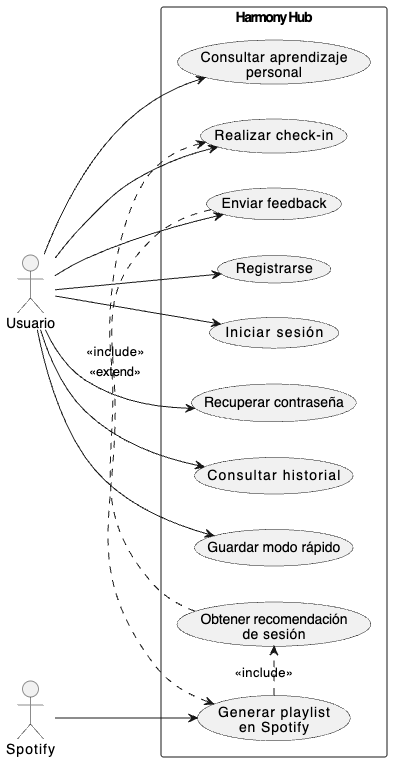
\includegraphics[width=0.52\linewidth]{Imagenes/diagrama_casos_uso.png}
    \caption{Diagrama general de casos de uso de Harmony Hub.}
    \label{fig:casos_uso_general}
\end{figure}

\subsection*{Casos de uso principales descritos}

Siguiendo el orden funcional del sistema, conviene resumir primero el acceso,
después la vinculación con Spotify, a continuación el flujo principal de sesión
y, por último, las funcionalidades de seguimiento, memoria y aprendizaje. Para
facilitar la lectura y la referencia cruzada posterior, cada caso de uso
principal se recoge en una tabla independiente y se acompaña de su diagrama
específico.

\begin{table}[H]
\centering
\small
\renewcommand{\arraystretch}{1.1}
\begin{tabularx}{\textwidth}{|P{1.1cm}|P{2.8cm}|P{1.4cm}|P{3.4cm}|Y|}
\hline
\textbf{ID} & \textbf{Caso de uso} & \textbf{Actor} & \textbf{Precondición} & \textbf{Resultado esperado} \\
\hline
CU1 & Registrarse e iniciar sesión & Usuario & El usuario dispone de la app y no mantiene sesión válida activa. & Se crea o valida la cuenta y se habilita el acceso a la pantalla principal. \\
\hline
\end{tabularx}
\caption{Caso de uso CU1: registrarse e iniciar sesión.}
\label{tab:caso_uso_cu1}
\end{table}

\begin{figure}[H]
    \centering
    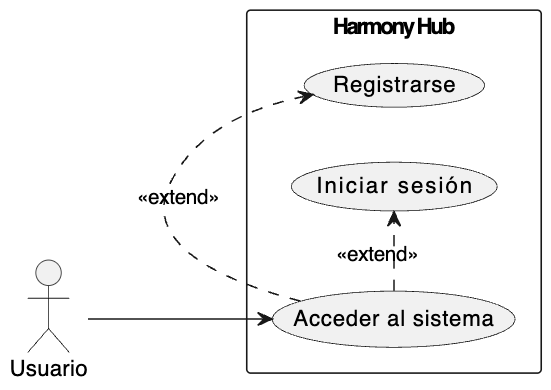
\includegraphics[width=0.54\linewidth]{Imagenes/caso_uso_cu1.png}
    \caption{Diagrama específico del caso de uso CU1: registrarse e iniciar sesión.}
    \label{fig:caso_uso_cu1}
\end{figure}

\begin{table}[H]
\centering
\small
\renewcommand{\arraystretch}{1.1}
\begin{tabularx}{\textwidth}{|P{1.1cm}|P{2.8cm}|P{1.4cm}|P{3.4cm}|Y|}
\hline
\textbf{ID} & \textbf{Caso de uso} & \textbf{Actor} & \textbf{Precondición} & \textbf{Resultado esperado} \\
\hline
CU2 & Recuperar contraseña & Usuario & El usuario ha olvidado la contraseña, pero recuerda el correo asociado. & El sistema envía el enlace de restablecimiento y la cuenta sigue siendo recuperable. \\
\hline
\end{tabularx}
\caption{Caso de uso CU2: recuperar contraseña.}
\label{tab:caso_uso_cu2}
\end{table}

\begin{figure}[H]
    \centering
    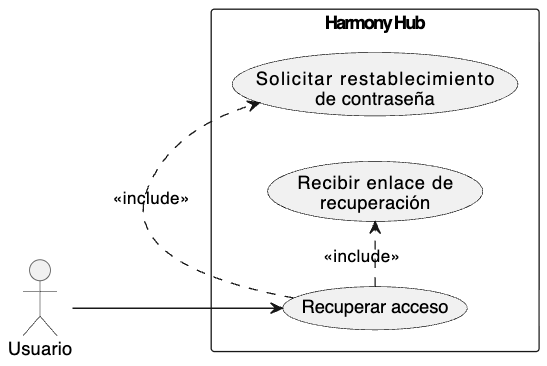
\includegraphics[width=0.54\linewidth]{Imagenes/caso_uso_cu2.png}
    \caption{Diagrama específico del caso de uso CU2: recuperar contraseña.}
    \label{fig:caso_uso_cu2}
\end{figure}

\begin{table}[H]
\centering
\small
\renewcommand{\arraystretch}{1.1}
\begin{tabularx}{\textwidth}{|P{1.1cm}|P{2.8cm}|P{1.4cm}|P{3.4cm}|Y|}
\hline
\textbf{ID} & \textbf{Caso de uso} & \textbf{Actor} & \textbf{Precondición} & \textbf{Resultado esperado} \\
\hline
CU3 & Conectar cuenta con Spotify & Usuario & El usuario ha iniciado sesión en Harmony Hub y todavía no ha vinculado su cuenta musical. & La cuenta de Spotify queda autorizada y disponible para generar playlists reales. \\
\hline
\end{tabularx}
\caption{Caso de uso CU3: conectar cuenta con Spotify.}
\label{tab:caso_uso_cu3}
\end{table}

\begin{figure}[H]
    \centering
    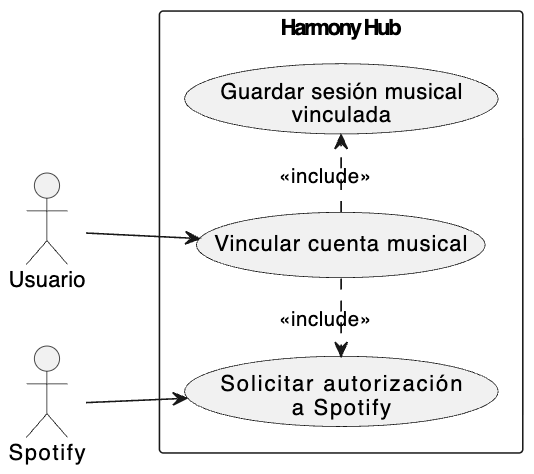
\includegraphics[width=0.54\linewidth]{Imagenes/caso_uso_cu3.png}
    \caption{Diagrama específico del caso de uso CU3: conectar cuenta con Spotify.}
    \label{fig:caso_uso_cu3}
\end{figure}

\begin{table}[H]
\centering
\small
\renewcommand{\arraystretch}{1.1}
\begin{tabularx}{\textwidth}{|P{1.1cm}|P{2.8cm}|P{1.4cm}|P{3.4cm}|Y|}
\hline
\textbf{ID} & \textbf{Caso de uso} & \textbf{Actor} & \textbf{Precondición} & \textbf{Resultado esperado} \\
\hline
CU4 & Realizar una sesión musical contextual & Usuario & El usuario ha iniciado sesión y tiene acceso operativo a la app. & Se registra el check-in, se genera la recomendación y se crea una playlist trazable. \\
\hline
\end{tabularx}
\caption{Caso de uso CU4: realizar una sesión musical contextual.}
\label{tab:caso_uso_cu4}
\end{table}

\begin{figure}[H]
    \centering
    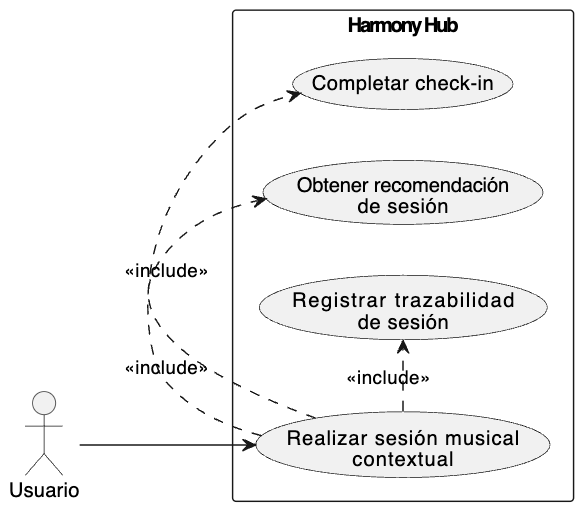
\includegraphics[width=0.54\linewidth]{Imagenes/caso_uso_cu4.png}
    \caption{Diagrama específico del caso de uso CU4: realizar una sesión musical contextual.}
    \label{fig:caso_uso_cu4}
\end{figure}

\begin{table}[H]
\centering
\small
\renewcommand{\arraystretch}{1.1}
\begin{tabularx}{\textwidth}{|P{1.1cm}|P{2.8cm}|P{1.4cm}|P{3.4cm}|Y|}
\hline
\textbf{ID} & \textbf{Caso de uso} & \textbf{Actor} & \textbf{Precondición} & \textbf{Resultado esperado} \\
\hline
CU5 & Consultar historial personal & Usuario & Existen sesiones registradas previamente. & El usuario puede revisar check-ins, playlists y feedback asociados. \\
\hline
\end{tabularx}
\caption{Caso de uso CU5: consultar historial personal.}
\label{tab:caso_uso_cu5}
\end{table}

\begin{figure}[H]
    \centering
    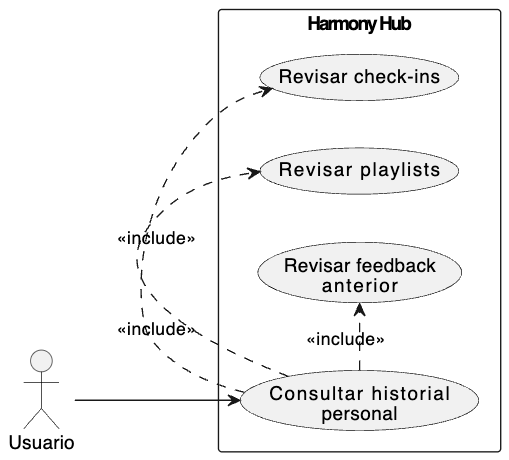
\includegraphics[width=0.54\linewidth]{Imagenes/caso_uso_cu5.png}
    \caption{Diagrama específico del caso de uso CU5: consultar historial personal.}
    \label{fig:caso_uso_cu5}
\end{figure}

\begin{table}[H]
\centering
\small
\renewcommand{\arraystretch}{1.1}
\begin{tabularx}{\textwidth}{|P{1.1cm}|P{2.8cm}|P{1.4cm}|P{3.4cm}|Y|}
\hline
\textbf{ID} & \textbf{Caso de uso} & \textbf{Actor} & \textbf{Precondición} & \textbf{Resultado esperado} \\
\hline
CU6 & Guardar un modo rápido & Usuario & El usuario navega por la sección de modos y detecta una situación reutilizable. & El modo queda almacenado como acceso rápido para uso posterior. \\
\hline
\end{tabularx}
\caption{Caso de uso CU6: guardar un modo rápido.}
\label{tab:caso_uso_cu6}
\end{table}

\begin{figure}[H]
    \centering
    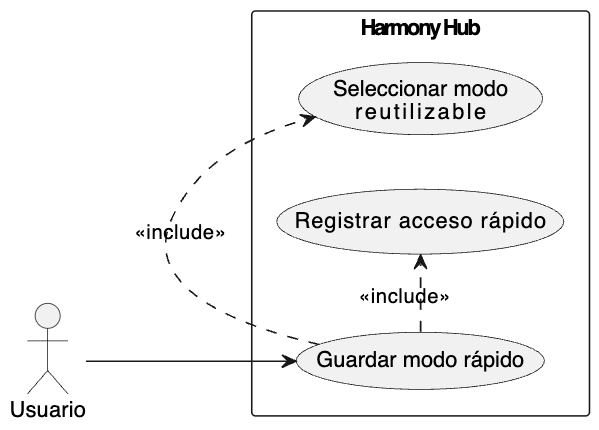
\includegraphics[width=0.54\linewidth]{Imagenes/caso_uso_cu6.png}
    \caption{Diagrama específico del caso de uso CU6: guardar un modo rápido.}
    \label{fig:caso_uso_cu6}
\end{figure}

\begin{table}[H]
\centering
\small
\renewcommand{\arraystretch}{1.1}
\begin{tabularx}{\textwidth}{|P{1.1cm}|P{2.8cm}|P{1.4cm}|P{3.4cm}|Y|}
\hline
\textbf{ID} & \textbf{Caso de uso} & \textbf{Actor} & \textbf{Precondición} & \textbf{Resultado esperado} \\
\hline
CU7 & Enviar feedback sobre una sesión & Usuario & Existe una recomendación o playlist generada asociada a la sesión. & La sesión queda cerrada con valoración y disponible para aprendizaje posterior. \\
\hline
\end{tabularx}
\caption{Caso de uso CU7: enviar feedback sobre una sesión.}
\label{tab:caso_uso_cu7}
\end{table}

\begin{figure}[H]
    \centering
    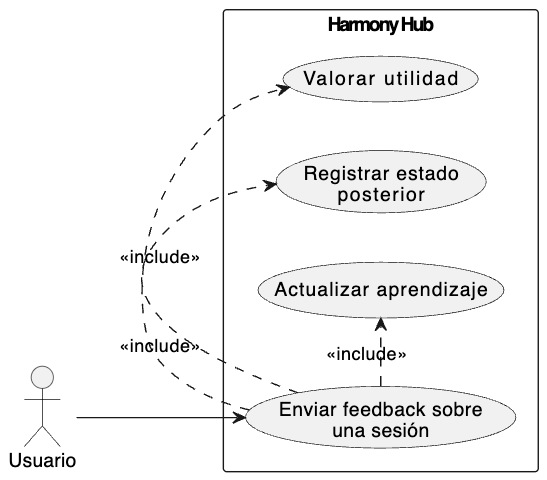
\includegraphics[width=0.54\linewidth]{Imagenes/caso_uso_cu7.png}
    \caption{Diagrama específico del caso de uso CU7: enviar feedback sobre una sesión.}
    \label{fig:caso_uso_cu7}
\end{figure}

\begin{table}[H]
\centering
\small
\renewcommand{\arraystretch}{1.1}
\begin{tabularx}{\textwidth}{|P{1.1cm}|P{2.8cm}|P{1.4cm}|P{3.4cm}|Y|}
\hline
\textbf{ID} & \textbf{Caso de uso} & \textbf{Actor} & \textbf{Precondición} & \textbf{Resultado esperado} \\
\hline
CU8 & Consultar aprendizaje personal & Usuario & Existe actividad previa suficiente dentro del sistema. & El usuario accede a patrones e insights agregados sobre su historial de uso. \\
\hline
\end{tabularx}
\caption{Caso de uso CU8: consultar aprendizaje personal.}
\label{tab:caso_uso_cu8}
\end{table}

\begin{figure}[H]
    \centering
    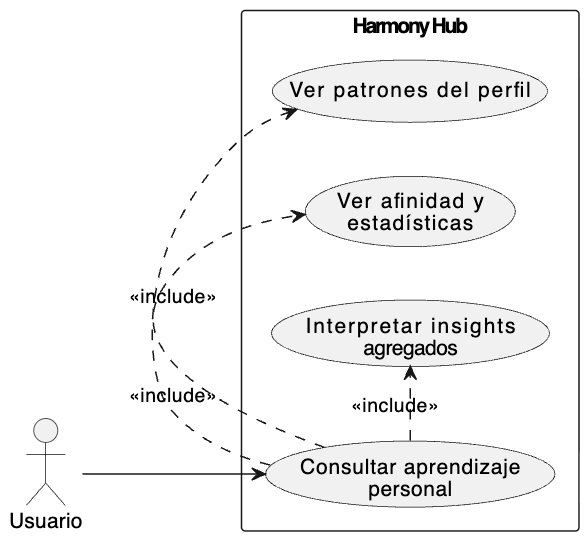
\includegraphics[width=0.54\linewidth]{Imagenes/caso_uso_cu8.png}
    \caption{Diagrama específico del caso de uso CU8: consultar aprendizaje personal.}
    \label{fig:caso_uso_cu8}
\end{figure}

\section{Matriz de trazabilidad}
\label{sec:matriz_trazabilidad}

Para reforzar la coherencia entre el análisis funcional y el comportamiento
esperado del sistema, la Tabla~\ref{tab:matriz_trazabilidad} reorganiza la
trazabilidad desde el punto de vista de los casos de uso principales. Para
facilitar la lectura, la matriz reduce la información a la relación directa
entre caso de uso y requisito, marcando con una X las coincidencias
correspondientes.

\begin{table}[H]
\centering
\scriptsize
\renewcommand{\arraystretch}{1.1}
\setlength{\tabcolsep}{2.8pt}
\resizebox{\textwidth}{!}{%
\begin{tabular}{|c|*{12}{c|}*{9}{c|}}
\hline
\textbf{CU} & \textbf{RF1} & \textbf{RF2} & \textbf{RF3} & \textbf{RF4} & \textbf{RF5} & \textbf{RF6} & \textbf{RF7} & \textbf{RF8} & \textbf{RF9} & \textbf{RF10} & \textbf{RF11} & \textbf{RF12} & \textbf{RNF1} & \textbf{RNF2} & \textbf{RNF3} & \textbf{RNF4} & \textbf{RNF5} & \textbf{RNF6} & \textbf{RNF7} & \textbf{RNF8} & \textbf{RNF9} \\
\hline
CU1 & X &  &  &  &  &  &  &  &  &  &  &  & X &  &  & X &  & X &  &  &  \\
\hline
CU2 &  & X &  &  &  &  &  &  &  &  &  &  & X &  &  & X &  &  &  &  &  \\
\hline
CU3 &  &  &  &  &  &  & X &  &  &  &  &  & X &  &  &  & X & X &  &  &  \\
\hline
CU4 &  &  & X & X & X & X &  & X &  &  &  &  & X & X & X &  & X &  &  & X & X \\
\hline
CU5 &  &  &  &  &  & X &  &  & X & X &  &  & X &  & X & X &  &  &  &  &  \\
\hline
CU6 &  &  &  &  &  &  &  &  &  &  &  & X & X &  &  &  &  & X &  &  &  \\
\hline
CU7 &  &  &  &  &  & X &  &  &  & X & X &  & X &  & X & X &  &  &  &  & X \\
\hline
CU8 &  &  &  &  &  &  &  &  & X &  & X &  & X &  &  &  &  &  &  & X & X \\
\hline
\end{tabular}}
\caption{Matriz de trazabilidad centrada en casos de uso y requisitos.}
\label{tab:matriz_trazabilidad}
\end{table}

\section{Restricciones y riesgos iniciales}
\label{sec:restricciones_riesgos}

El diseño de Harmony Hub está condicionado por varias restricciones que conviene reconocer desde el principio, ya que afectan tanto a la implementación como a la evaluación del sistema.

\textbf{Restricciones técnicas}
\begin{itemize}
    \item La integración con Spotify depende de permisos, disponibilidad y cambios en su API.
    \item Algunas capacidades avanzadas del ecosistema Spotify no siempre están disponibles en modo de desarrollo o pueden sufrir restricciones externas.
    \item La experiencia debe funcionar en móvil sin requerir sensores complejos ni hardware específico.
    \item El sistema de aprendizaje no puede asumirse como plenamente operativo desde el inicio, porque depende de disponer de suficiente volumen y equilibrio de datos etiquetados.
    \item La persistencia documental depende de reglas activas de Firestore y de la coherencia entre dichas reglas, los documentos generados por el cliente y los agregados escritos por backend.
    \item El análisis acústico del entorno debe limitarse a métricas resumidas y no a audio persistido, lo que restringe deliberadamente la profundidad del tratamiento posible sobre la señal.
\end{itemize}

\textbf{Restricciones de alcance}
\begin{itemize}
    \item El proyecto debe mantenerse dentro del marco temporal y técnico de un TFG.
    \item No se persigue construir un producto clínico, ni validar resultados terapéuticos, ni desarrollar un sistema musical universal.
    \item El aprendizaje se plantea a nivel de sesión, no como un modelo total de predicción del comportamiento musical del usuario.
    \item La evaluación longitudinal se concentra en un perfil principal de uso, lo que favorece la trazabilidad del aprendizaje pero limita la comparación entre perfiles heterogéneos.
\end{itemize}

\textbf{Riesgos iniciales}
\begin{itemize}
    \item \textbf{R1. Dependencia de servicios externos}. Si Spotify cambia un endpoint o restringe funcionalidades, parte del flujo puede verse afectado.
    \item \textbf{Mitigación}. Diseñar la arquitectura para que el backend mantenga el ranking principal sobre un catálogo propio y deje a Spotify sobre todo la fase de materialización final.
    \item \textbf{R2. Insuficiencia de datos para activar el modelo}. Un volumen bajo o desequilibrado de feedback puede impedir que el aprendizaje entre en producción con garantías.
    \item \textbf{Mitigación}. Mantener una puerta de activación objetiva y asegurar un modo heurístico funcional mientras se recopilan datos.
    \item \textbf{R3. Fricción de uso}. Si el check-in es demasiado largo o el flujo resulta poco claro, el usuario puede abandonar antes de cerrar la sesión con feedback.
    \item \textbf{Mitigación}. Priorizar una experiencia móvil breve, guiada y con jerarquía visual clara.
    \item \textbf{R4. Expectativas infladas sobre la personalización}. El usuario podría esperar una precisión muy alta desde las primeras sesiones.
    \item \textbf{Mitigación}. Diseñar el sistema como aprendizaje progresivo y dejar claro que mejora con el uso.
    \item \textbf{R5. Desalineación entre reglas documentales y cliente}. Un cambio menor en nombres de campos o colecciones puede bloquear escrituras críticas como feedback o persistencia privada.
    \item \textbf{Mitigación}. Mantener validaciones explícitas, revisar \texttt{firestore.rules} junto con los servicios Flutter y comprobar el flujo completo con pruebas manuales de extremo a extremo.
    \item \textbf{R6. Cobertura insuficiente del catálogo local}. Un catálogo estructurado todavía limitado puede dejar algunos contextos con menor variedad o con materialización más difícil en Spotify.
    \item \textbf{Mitigación}. Enriquecer progresivamente \texttt{msd\_tracks}, documentar mecanismos de \textit{fallback} y mantener la separación entre ranking local y materialización externa.
\end{itemize}

En conjunto, estas restricciones no invalidan la solución. Ayudan a situarla con mayor precisión y a distinguir entre lo que el sistema ya resuelve, lo que resuelve parcialmente y lo que queda como evolución futura.

\chapter{Diseño de la solución}
\label{ch:diseno_solucion}

% Este capítulo cubre el apartado "Diseño" de la guía: modelos de datos, arquitectura,
% interfaz, funcionalidad, pruebas y justificación de decisiones.

\section{Vista general de la solución}
\label{sec:vista_general_solucion}

Harmony Hub se ha diseñado como una solución distribuida y modular, en la que
la aplicación móvil actúa como punto de interacción principal con el usuario,
mientras que el backend concentra la lógica de recomendación, la coordinación
del aprendizaje y la comunicación con Spotify. Además, Firestore se utiliza
como capa de persistencia flexible para almacenar sesiones, recomendaciones,
playlists generadas, feedback y estructuras auxiliares de aprendizaje.

En términos generales, el flujo de la solución es el siguiente: el usuario
realiza un check-in breve desde la app, el backend interpreta ese contexto y
genera una recomendación de sesión, la aplicación puede traducir esa propuesta
a una playlist real en Spotify y, finalmente, el feedback recogido permite
conservar trazabilidad y mejorar la personalización progresiva del sistema.

\section{Arquitectura del sistema}
\label{sec:arquitectura}

La arquitectura elegida separa con bastante claridad las responsabilidades del
sistema. La aplicación móvil, desarrollada en Flutter, se encarga de la
interfaz, la captura del contexto de sesión y parte de la persistencia del lado
cliente. El backend, implementado con FastAPI, recibe el contexto, genera la
recomendación, coordina la lógica adaptativa y media en la integración con
Spotify. Por último, Firestore funciona como soporte de persistencia documental,
algo especialmente útil en un sistema donde conviven documentos públicos,
bloques privados cifrados e información incremental de aprendizaje.

Esta arquitectura no se planteó solo para repartir tecnologías, sino para
ordenar con claridad el flujo de datos del proyecto. Harmony Hub necesita
combinar interacción móvil, servicios externos, persistencia documental y una
capa de recomendación con aprendizaje progresivo. Por eso resulta importante
que cada componente tenga una responsabilidad bien delimitada y que la
comunicación entre ellos sea comprensible tanto a nivel funcional como a nivel
técnico.

La aplicación móvil actúa como puerta de entrada del contexto: recoge el
check-in, activa opcionalmente la medición del entorno y muestra la respuesta
final al usuario. El backend recibe esa información, genera candidatos de modo,
aplica la lógica heurística y, si corresponde, permite intervenir al modelo
supervisado de sesión. Firestore conserva el historial, las playlists, el
feedback, los perfiles aprendidos y los artefactos auxiliares necesarios para
la trazabilidad. Spotify queda situado en la fase de autenticación musical y en
la materialización final de playlists, no en la toma principal de decisiones
musicales.

La Figura~\ref{fig:arquitectura_harmony_hub} resume esta organización y
visibiliza tanto los componentes principales como las direcciones de flujo entre
ellos.

\begin{figure}[htbp]
\centering
\begingroup
\shorthandoff{<>}
\begin{tikzpicture}[
    node distance=1.1cm and 1.3cm,
    box/.style={draw, rounded corners=2pt, align=center, text width=3.6cm, minimum height=1.6cm, fill=gray!10},
    data/.style={draw, rounded corners=2pt, align=center, text width=3.6cm, minimum height=1.5cm, fill=cyan!10},
    ext/.style={draw, rounded corners=2pt, align=center, text width=3.6cm, minimum height=1.5cm, fill=green!10},
    flow/.style={->, thick}
]
\node[box] (app) {\textbf{Aplicación móvil Flutter}\\check-in, navegación, feedback\\y medición opcional del entorno};
\node[data, below=0.1cm of app] (context) {\textbf{Contexto de sesión}\\estado de ánimo, energía, estrés\\preferencias y entorno};

\node[box, right=1.5cm of app] (backend) {\textbf{Backend FastAPI}\\API REST, orquestación\\integración y trazabilidad};
\node[box, below=0.1cm of backend] (engine) {\textbf{Motor híbrido}\\heurística, catálogo y ML\\selección de modo};

\node[data, right=1.5cm of backend] (firestore) {\textbf{Cloud Firestore}\\sesiones, playlists, feedback\\perfiles y ejemplos};
\node[ext, below=0.1cm of firestore] (spotify) {\textbf{Spotify Web API}\\OAuth y PKCE\\materialización de playlists};

\draw[flow] (app) -- (backend);
\draw[flow] (app) -- (context);
\draw[flow] (context) -- (engine);
\draw[flow] (backend) -- (engine);
\draw[flow] (engine) -- (spotify);
\draw[<->, thick] (backend) -- (firestore);
\draw[<->, thick] (engine) -- (firestore);
\end{tikzpicture}
\endgroup
\caption{Arquitectura general de Harmony Hub y flujo principal entre sus componentes.}
\label{fig:arquitectura_harmony_hub}
\end{figure}

Desde el punto de vista del flujo de datos, el recorrido principal puede
describirse en seis pasos: captura del check-in en la app, envío del contexto
al backend, generación de la recomendación sobre el catálogo propio, consulta y
actualización de persistencia en Firestore, materialización de la playlist en
Spotify y devolución del resultado al usuario junto con la recogida posterior
de feedback. Esta secuencia es importante porque deja claro que el sistema no
es únicamente una interfaz conectada a una API externa, sino una solución
distribuida donde la decisión principal se produce dentro de la lógica propia
del proyecto.

\section{Diseño modular y separación de responsabilidades}
\label{sec:diseno_modular}

La modularidad no se introdujo solo como una preferencia de implementación,
sino como una condición práctica para mantener la solución evolucionable.
Harmony Hub combina interfaz móvil, backend, persistencia documental,
integración externa y aprendizaje supervisado; si toda esa lógica se
concentrara en una sola capa, cualquier cambio en Spotify, en el flujo de
feedback o en el modelo de sesión terminaría afectando a demasiadas piezas a la
vez.

Por esa razón, el diseño se apoya en módulos relativamente desacoplados, con
fronteras funcionales bastante claras:

\begin{table}[H]
\centering
\small
\renewcommand{\arraystretch}{1.1}
\begin{tabularx}{\textwidth}{|P{2.8cm}|P{3.4cm}|Y|}
\hline
\textbf{Módulo} & \textbf{Ubicación principal} & \textbf{Responsabilidad} \\
\hline
Interfaz móvil & Flutter & Captura del check-in, navegación, visualización de recomendaciones, historial, feedback y perfil. \\
\hline
Servicios de cliente & Flutter & Orquestación de llamadas al backend, persistencia documental mínima en Firestore y cifrado local de bloques sensibles. \\
\hline
Motor de recomendación & FastAPI & Transformación del contexto de sesión en una propuesta musical, construcción del perfil funcional y ranking principal sobre el catálogo propio msd\_tracks. \\
\hline
Integración con Spotify & FastAPI + app móvil & Autenticación mediante PKCE, lectura del perfil musical básico y materialización final de playlists reales. \\
\hline
Persistencia documental & Firestore & Almacenamiento de check-ins, recomendaciones, playlists generadas, feedback, perfiles de aprendizaje y ejemplos de entrenamiento. \\
\hline
Aprendizaje supervisado & Backend ML & Reordenado opcional de modos candidatos cuando existen suficientes datos y métricas objetivas de calidad. \\
\hline
\end{tabularx}
\caption{Organización modular de Harmony Hub y responsabilidades principales.}
\label{tab:diseno_modular}
\end{table}

Esta separación aporta tres ventajas concretas. En primer lugar, permite que la
experiencia móvil siga siendo usable aunque el modelo supervisado todavía no
esté activado. En segundo lugar, facilita introducir cambios en la integración
con Spotify sin reestructurar el resto de la app. Y, por último, hace posible
documentar, probar y evolucionar cada bloque con mayor precisión técnica.

\section{Diseño del motor de recomendación e integración con Spotify}
\label{sec:diseno_motor_recomendacion}

El corazón funcional de Harmony Hub no está en una sola pantalla ni en una sola
consulta a Spotify, sino en una cadena de decisiones que convierte un contexto
personal en una escucha real. Por eso conviene describir el motor de
recomendación y la integración con Spotify como un diseño conjunto: el primero
decide qué tipo de sesión conviene, y la segunda se encarga de materializar esa
propuesta en una playlist reproducible.

\subsection{Diseño del motor de recomendación}

El motor de recomendación trabaja por niveles. Primero interpreta el check-in
del usuario como un contexto de sesión; después genera varios candidatos de
modo; finalmente, selecciona el que mejor encaja y lo transforma en un perfil
musical utilizable por la capa Spotify.

De forma resumida, el flujo interno sigue estas etapas:

\begin{enumerate}
    \item captura del contexto declarado por el usuario: estado de ánimo, objetivo, energía, estrés, preferencias de sesión y, cuando procede, resumen acústico del entorno;
    \item generación de candidatos de sesión combinando objetivo, momento emocional e intensidad prevista;
    \item puntuación heurística de esos candidatos con reglas de coherencia funcional y restricciones de contexto;
    \item reordenado opcional mediante el modelo supervisado de sesión, si este ha superado sus puertas de datos y calidad global;
    \item construcción de un perfil final de generación con atributos como el modo recomendado, la energía objetivo, la valencia objetivo y el rango de pulso estimado;
    \item entrega de ese perfil al pipeline musical para recuperar y rankear candidatos en msd\_tracks y, posteriormente, materializar la playlist final en Spotify.
\end{enumerate}

Desde un punto de vista académico, el sistema no recomienda canciones
directamente a partir de un gran modelo global, sino que opera como un motor
híbrido. La heurística garantiza funcionamiento desde el primer día, mientras
que la capa supervisada solo entra cuando hay evidencia suficiente para hacerlo
con garantías. Esa evidencia se mide en dos planos: una puerta global de datos
y calidad del modelo, y una confianza mínima en la sesión concreta antes de
permitir la reordenación supervisada.
Desde el punto de vista del usuario, esto se traduce en una idea mucho más
sencilla: la app siempre puede proponer una sesión útil, pero solo incorpora lo
aprendido cuando realmente tiene base para ello.

Conviene distinguir, además, dos mecanismos de aprendizaje que no deben
confundirse. Por un lado, existe un aprendizaje individual del perfil del
usuario, basado en pesos contextuales y estables que pueden madurar antes y que
ya influyen en la generación musical mediante modos como
\texttt{progressive\_contextual} o \texttt{stable\_weighted}. Por otro lado,
existe un clasificador supervisado global de sesión, sometido a puertas de
datos y calidad más exigentes. Esta separación explica por qué el sistema puede mostrar
aprendizaje útil y visible en la experiencia final aunque el modelo global siga
absteniéndose de intervenir.

\subsection{Puntuación heurística, coherencia funcional y restricciones de contexto}

La puntuación heurística es la primera capa de decisión real del sistema. Su
papel consiste en valorar si un candidato de sesión es coherente con el momento
de la persona antes de acudir, si procede, al reordenado supervisado. No es una
heurística arbitraria: se apoya en reglas de compatibilidad funcional entre el
objetivo del usuario, su estado actual, sus preferencias y las limitaciones del
contexto externo. Esta lógica se implementa después en el backend, tal y como
se describe en la Sub\-sección~\ref{subsec:modulo_recomendacion_implementacion}.

De forma resumida, la puntuación heurística combina varias familias de señales:

\begin{itemize}
    \item \textbf{Compatibilidad base entre objetivo y modo candidato}. Un modo
    de relajación se considera más coherente para objetivos de calma, uno de
    foco para tareas de concentración y uno de energía para necesidades de
    activación.
    \item \textbf{Distancia respecto a la intensidad pedida}. Si el usuario
    solicita una sesión suave, un candidato alta pierde
    puntuación; si la preferencia es media, las variantes vecinas quedan
    mejor posicionadas que las extremas.
    \item \textbf{Coherencia con el estado declarado}. Estrés alto, energía muy
    baja o necesidad de acabar más calmado modifican la conveniencia de
    cada tipo de sesión.
    \item \textbf{Adecuación al entorno}. Si se activa el uso del contexto
    acústico, el sistema incorpora restricciones asociadas al nivel de ruido
    medido y a la necesidad de que la música acompañe o se imponga al entorno.
    \item \textbf{Restricciones musicales explícitas}. Preferencia
    instrumental, exploración más segura, popularidad esperada o veto implícito
    a canciones excesivamente agresivas, explícitas o tensas en ciertos
    contextos.
\end{itemize}

Estas señales se traducen en reglas de coherencia funcional. Por ejemplo, en una
sesión de relajación se penalizan candidatos demasiado activados o con
poca estabilidad; en una sesión de foco se favorecen perfiles
instrumentales y se endurecen incompatibilidades con letras, explicitud o
exceso de tensión; en una sesión de energía se buscan señales de
activación y valencia suficientemente positivas, pero evitando saltos bruscos
cuando el usuario se encuentra especialmente cansado.

Del mismo modo, aparecen restricciones de contexto que limitan la decisión
aunque un candidato parezca inicialmente plausible. Un ejemplo claro es la
preferencia vocal instrumental: si el usuario pide instrumentales, el motor no
debe tratar por igual un candidato que dependa de canciones vocales. Otro caso
es la necesidad de no depender de búsquedas externas para cada decisión fina.
Por eso, la solución se apoya en un catálogo estructurado propio,
msd\_tracks, que actúa como fuente principal de canciones candidatas y
de descriptores musicales normalizados. Spotify se reserva para la
materialización final de URIs reproducibles, mientras que la lógica de ranking
se apoya sobre atributos ya preparados en el catálogo, afinidad histórica y
señales semánticas.

La Tabla~\ref{tab:heuristica_contexto} resume estas reglas de diseño:

\begin{table}[H]
\centering
\small
\renewcommand{\arraystretch}{1.1}
\begin{tabularx}{\textwidth}{|P{3.1cm}|Y|Y|}
\hline
\textbf{Familia de regla} & \textbf{Criterio aplicado} & \textbf{Efecto esperado} \\
\hline
Coherencia objetivo--modo & Se premian combinaciones compatibles entre objetivo de sesión y modo candidato. & Reduce recomendaciones que no responden al propósito principal del usuario. \\
\hline
Preferencia de intensidad & Se compara la intensidad solicitada con la intensidad del candidato. & Favorece que la sesión se sienta proporcionada al momento. \\
\hline
Estado emocional y funcional & Estrés, energía y resultado deseado ajustan la puntuación base. & Mejora la pertinencia situacional de la recomendación. \\
\hline
Restricciones de entorno & El ruido y el uso del entorno limitan o refuerzan ciertos perfiles musicales. & Ayuda a que la sesión no se desconecte del contexto real de escucha. \\
\hline
Restricciones musicales & Preferencia instrumental, exploración o reglas contra explicitud y tensión. & Evita candidatos funcionalmente incompatibles aunque encajen por afinidad musical. \\
\hline
Catálogo MSD como base & El ranking utiliza descriptores locales, etiquetas semánticas y campos funcionales del catálogo msd\_tracks. & Reduce dependencia de llamadas externas y mantiene coherencia musical estable entre sesiones. \\
\hline
\end{tabularx}
\caption{Reglas de puntuación heurística, coherencia funcional y restricciones de contexto.}
\label{tab:heuristica_contexto}
\end{table}

La Lista~\ref{lst:pseudocodigo_recomendacion} resume este comportamiento en
forma de pseudocódigo de alto nivel.

\begin{listing}[H]
\begin{minted}[fontsize=\small,breaklines]{text}
ALGORITMO RecomendarSesionYPlaylist(contexto_usuario)
  recibir estado de animo, objetivo, energia, estres, preferencias y entorno
  generar candidatos de modo combinando objetivo, momento e intensidad

  PARA cada candidato HACER
    score <- score_base_por_objetivo_y_modo(candidato, contexto_usuario)
    score <- score + ajuste_por_intensidad(candidato, contexto_usuario)
    score <- score + ajuste_por_estres_y_energia(candidato, contexto_usuario)
    score <- score + ajuste_por_resultado_deseado(candidato, contexto_usuario)
    score <- score + ajuste_por_entorno(candidato, contexto_usuario)
    score <- score + ajuste_por_preferencias_musicales(candidato, contexto_usuario)
  FIN PARA

  SI modelo_supervisado_disponible(contexto_usuario) ENTONCES
    reordenar candidatos con probabilidad de utilidad aprendida
  FIN SI

  seleccionar mejor candidato
  construir perfil musical final
  recuperar canciones candidatas desde el catalogo MSD
  filtrar y puntuar canciones según coherencia funcional y restricciones activas
  resolver materializacion final en Spotify
  ensamblar playlist final
  devolver recomendacion, perfil y playlist
FIN ALGORITMO
\end{minted}
\caption{Pseudocódigo del algoritmo híbrido de recomendación de sesión y playlist.}
\label{lst:pseudocodigo_recomendacion}
\end{listing}

\subsection{Uso del catálogo MSD en la generación musical}

La base musical de Harmony Hub se apoya en un catálogo local estructurado en
\texttt{msd\_tracks}. Este catálogo deriva de una adaptación del
Million Song Dataset \cite{msd_2011} a las necesidades funcionales del
proyecto y se almacena como colección documental y como fuente local en formato
JSONL. En el estado
actual del sistema, el catálogo reúne 5\,441 pistas, lo que permite trabajar
con un espacio musical bastante más amplio y estable que el disponible en las
primeras iteraciones del prototipo. Cada pista incorpora, además de
identificadores y metadatos básicos, un conjunto de descriptores ya
normalizados: tempo, danceability, energía, valencia,
instrumentalidad, popularidad aproximada, género, etiquetas semánticas y
campos funcionales como \texttt{focus\_score}, \texttt{calm\_score},
\texttt{uplift\_score}, \texttt{warmth\_score}, \texttt{tension\_score} o
\texttt{supportiveness\_score}.

Conviene precisar que el nombre interno \texttt{msd\_tracks} se conserva por
continuidad arquitectónica, pero el catálogo final no es una copia literal del
Million Song Dataset. Se trata de un recurso híbrido: parte de una base
conceptual inspirada en MSD y la amplía con procesos de normalización,
bootstrap y enriquecimiento funcional realizados dentro del propio proyecto
para mantener una estructura homogénea de rasgos musicales y etiquetas
operativas.

Esta decisión tiene dos ventajas importantes. La primera es arquitectónica: el
motor puede puntuar candidatos con un conjunto de señales homogéneo, sin quedar
condicionado por la disponibilidad variable de endpoints externos. La segunda
es metodológica: la lógica de recomendación se vuelve trazable y reproducible,
porque la selección no depende de datos opacos recuperados en tiempo real, sino
de un repositorio estable sobre el que pueden explicarse reglas, pesos y
descriptores.

Desde el punto de vista metodológico, el script de generación musical no parte
de una única fuente cerrada, sino de la combinación de varias ideas asentadas
en recomendación musical. La primera es el uso de catálogos ricos en metadatos
y descriptores acústicos para sostener recomendación \textit{content-based}, en
línea con la tradición resumida por Deldjoo, Schedl y Knees
\cite{deldjoo_2021_contentdriven}. La segunda es entender la playlist como una
secuencia con función y orden interno, no solo como un conjunto de pistas
intercambiables, algo coherente con la literatura sobre generación automática
de playlists y orden de canciones \cite{vall_2018_playlist_order}. La tercera
es la preferencia por señales interpretables —género, energía, valencia,
instrumentalidad, calidez o soporte emocional— frente a una recuperación
puramente opaca, una dirección también alineada con trabajos sobre
recomendación musical transparente apoyada en features explicables
\cite{lee_2018_transparent_music}. Sobre esas bases, Harmony Hub implementa una
solución propia centrada en regulación emocional y trazabilidad funcional.

En la práctica, el flujo es el siguiente: el sistema construye un perfil de
sesión, selecciona candidatos del catálogo MSD con ayuda de géneros semilla,
consultas principales y afinidad del usuario, y solo al final intenta
materializar esas pistas como canciones reproducibles en Spotify. De este modo,
Spotify actúa como plataforma de ejecución de la playlist, mientras que la
decisión musical principal se toma sobre un espacio controlado por el propio
proyecto.

Los géneros semilla cumplen aquí una función de orientación, no de selección
directa. Delimitan la zona musical sobre la que el sistema trabaja antes del
ranking fino y ayudan a decidir si conviene explorar un espacio más próximo a
\texttt{ambient}, \texttt{chill}, \texttt{classical}, \texttt{indie} o
\texttt{electronic}. Para ello combinan géneros base del objetivo, géneros
aprendidos de la sesión reciente y géneros aprendidos del perfil estable. En
Harmony Hub ya no se utilizan como semillas de una
recuperación principal en Spotify, sino como parte del \textit{generation
profile} que orienta la selección sobre MSD y deja preparadas búsquedas de
apoyo únicamente cuando el sistema necesita mecanismos de \textit{fallback} o
\textit{rescue}.


\subsection{Ejemplo operativo del motor híbrido}

Un ejemplo representativo permite observar cómo cooperan la heurística, el
modelo supervisado y el catálogo MSD. Considérese un check-in con objetivo de
relajación, estado estresado, estrés alto, energía baja e intensidad
suave. A partir de esa entrada, el sistema genera varios candidatos de modo,
como \texttt{relajacion\_estresado\_}\allowbreak\texttt{suave},
\texttt{relajacion\_estresado\_}\allowbreak\texttt{media} y
\texttt{relajacion\_estresado\_}\allowbreak\texttt{alta}. La heurística sitúa
en primer lugar la
variante suave porque es la que mejor alinea objetivo, intensidad y resultado
deseado.

Si el clasificador supervisado está disponible y ha superado sus puertas de
datos y calidad, ese conjunto se reordena con probabilidades de utilidad
aprendida. Si no existe evidencia suficiente para activar el modelo global, el
sistema deja trazas de abstención y mantiene la decisión heurística. De forma
independiente, el perfil individual todavía puede aplicar una mezcla
progresiva de preferencias estables y contextuales cuando la evidencia local
del usuario resulta útil, evitando así el salto brusco entre ``todo
aprendido'' y ``nada aprendido''. En ambos casos, el resultado es un
\textit{generation profile} con atributos funcionales, por ejemplo géneros
semilla (\texttt{ambient}, \texttt{chill}, \texttt{classical}), consultas
principales (\texttt{soft ambient calm}, \texttt{quiet piano relax}) y
objetivos de valencia y energía.

Con ese perfil, el backend consulta el catálogo msd\_tracks, puntúa
las canciones según cercanía funcional y afinidad histórica, y obtiene una
lista ordenada de candidatas. Solo en el último paso esas pistas se intentan
materializar como URIs reales de Spotify. En consecuencia, ni el motor de
recomendación ni el componente ML eligen directamente canciones de Spotify,
sino que gobiernan la selección dentro de un catálogo musical controlado y
explicable.

Entre el modo de sesión genérico y el ranking concreto de canciones existe
además una capa intermedia de \textit{subtypes} funcionales. Esta capa permite
refinar el perfil musical cuando una misma combinación de objetivo, mood e
intensidad puede adquirir matices distintos según el resultado esperado o la
preferencia vocal. Así, el sistema no trata igual un caso de foco instrumental
orientado a concentración profunda que una sesión de foco con voz ligera y
acompañante. Este refinamiento incluye subtipos como
\texttt{deep\_focus}, \texttt{steady\_focus}, \texttt{guided\_focus},
\texttt{stable\_relaxation}, \texttt{comfort\_relaxation},
\texttt{warm\_relaxation}, \texttt{soft\_activation} o
\texttt{warm\_companionship}. Cada uno de ellos ajusta objetivos internos de
calidez, estabilidad, presencia vocal y curva temporal de la playlist, de modo
que la personalización no dependa solo del objetivo global, sino también del
tipo concreto de ayuda musical que se quiere ofrecer.

\begin{table}[H]
\centering
\small
\renewcommand{\arraystretch}{1.12}
\begin{tabularx}{\textwidth}{|P{2.9cm}|P{4.1cm}|Y|}
\hline
\textbf{Subtype} & \textbf{Situación típica} & \textbf{Sentido funcional} \\
\hline
\texttt{\seqsplit{deep\_focus}} & Foco, preferencia instrumental y resultado orientado a mayor concentración. & Prioriza baja distracción, presencia instrumental clara y energía contenida. \\
\hline
\texttt{\seqsplit{guided\_focus}} & Foco con preferencia \texttt{con\_voz} y necesidad de concentración o acompañamiento moderado. & Mantiene estructura y estabilidad, pero tolera una voz cálida y guiada siempre que no vuelva la sesión demasiado bailable o tensa. \\
\hline
\texttt{\seqsplit{steady\_focus}} & Foco sin requisitos especiales adicionales. & Busca una concentración sostenida y equilibrada. \\
\hline
\texttt{\seqsplit{stable\_relaxation}} & Relajación con deseo explícito de acabar más calmado. & Favorece calma estable, baja tensión y una curva de asentamiento progresivo. \\
\hline
\texttt{\seqsplit{comfort\_relaxation}} & Relajación con voz y matiz de calma o acompañamiento. & Introduce una relajación más cercana y cálida, con presencia vocal suficiente sin perder tono reparador. \\
\hline
\texttt{\seqsplit{warm\_relaxation}} & Relajación con resultado esperado de sentirse más acompañado. & Refuerza calidez emocional y sensación de compañía. \\
\hline
\texttt{\seqsplit{soft\_activation}} & Energía con intensidad suave y activación progresiva. & Eleva el impulso sin romper bruscamente el estado inicial del usuario. \\
\hline
\texttt{\seqsplit{warm\_companionship}} & Energía en usuario triste con deseo de sentirse más acompañado. & Combina activación moderada con cercanía emocional y presencia vocal más marcada. \\
\hline
\end{tabularx}
\caption{Subtipos funcionales internos utilizados para refinar el perfil musical de sesión.}
\label{tab:subtipos_funcionales_sesion}
\end{table}

\subsection{Diseño de integración con Spotify}

La integración con Spotify no se concibe como un elemento ornamental, sino como
la pieza que convierte la recomendación en una salida realmente utilizable. El
flujo de autorización se apoya en Authorization Code with PKCE, que es
el enfoque recomendado por Spotify para aplicaciones móviles donde el secreto
del cliente no puede almacenarse de forma segura \cite{spotify_pkce}.

Una vez autorizada la cuenta, la integración utiliza varias señales:

\begin{itemize}
    \item perfil básico del usuario de Spotify;
    \item información mínima de afinidad útil para contextualizar el perfil del usuario;
    \item resolución final de canciones candidatas a URIs reproducibles;
    \item creación final de la playlist y publicación en la cuenta del usuario.
\end{itemize}

El diseño también contempla degradación controlada. Si un endpoint concreto no
está disponible, si Spotify devuelve restricciones en modo de desarrollo, si
aparecen límites de cuota o rate limits, o si no pueden recuperarse
ciertas características avanzadas, el sistema mantiene intacta la fase central
de ranking sobre msd\_tracks y limita la dependencia externa a la
materialización final. Esta decisión es importante porque evita que la utilidad
completa de Harmony Hub dependa de un único punto de fragilidad externa.

\subsection{Modelo supervisado de sesión}
\label{subsec:modelo_ml_sesion}

El modelo de aprendizaje de Harmony Hub no intenta predecir la canción ideal,
sino estimar qué modo de sesión tiene más probabilidad de resultar útil para un
contexto concreto. La unidad de aprendizaje es, por tanto, la sesión cerrada
con feedback, no el track individual. Esa elección reduce bastante la
ambigüedad de la señal supervisada, porque el usuario valora la experiencia
completa y no cada canción por separado.

En la implementación actual se utiliza una regresión logística regularizada
\cite{sklearn_logistic_regression}, que recibe como entrada una mezcla de
variables numéricas, categóricas y binarias
relacionadas con el contexto de la sesión y con el candidato propuesto. Entre
ellas aparecen, por ejemplo, el nivel de estrés, el nivel de energía, el
objetivo, el estado de ánimo, la preferencia de intensidad, el modo candidato o
el rango de pulso estimado. La salida del modelo es una probabilidad de que ese
candidato sea útil, es decir, de que la sesión termine valorada como favorable.
En términos de implementación, esa salida se obtiene mediante la operación
\texttt{predict\_proba(...)} de la regresión logística. Dado un conjunto de
candidatos de sesión ya construidos, el backend transforma cada uno en un
vector de características y pide al clasificador la probabilidad asociada a la
clase positiva. Así, para una fila concreta, \texttt{predict\_proba(...)[1]}
no devuelve una etiqueta categórica cerrada, sino un valor continuo entre 0 y
1 que puede interpretarse como probabilidad estimada de que ese modo resulte
útil en el contexto actual. Por ejemplo, una probabilidad cercana a
\texttt{0.50} expresa neutralidad del modelo, mientras que valores como
\texttt{0.60}, \texttt{0.75} o \texttt{0.95} representan grados
progresivamente mayores de confianza a favor del candidato. Esta elección es
relevante porque permite integrar el clasificador en un pipeline híbrido: en
lugar de imponer una decisión binaria, el modelo aporta una intensidad de apoyo
que después puede convertirse en un ajuste gradual sobre la puntuación
heurística previa.

Académicamente, esto permite plantear el problema como una clasificación
binaria a nivel de sesión. Operativamente, el backend utiliza esa probabilidad
para reordenar candidatos que ya habían sido prefiltrados por la heurística
base. No se trata de sustituir por completo el motor previo, sino de introducir
una capa de evidencia aprendida que empuja ligeramente hacia candidatos que
históricamente han funcionado mejor en contextos comparables.

En la implementación actual, esa intervención no se aplica como una sustitución
binaria, sino como un ajuste escalar sobre la puntuación heurística previa. Si
la probabilidad estimada para un candidato se denota por \(p\), el backend
calcula un incremento supervisado del tipo:
\[
\texttt{ml\_delta} = (p - 0.5) \cdot 10 \cdot w_{ml},
\]
donde \(w_{ml}\) es el peso operativo del componente supervisado. Con esta
regla, una probabilidad de \(0.50\) produce un ajuste nulo, una probabilidad
superior genera un refuerzo positivo y una probabilidad inferior lo convierte
en penalización. La puntuación final que se usa para ordenar candidatos deja de
ser, por tanto, solo heurística y pasa a calcularse como:
\[
\texttt{score\_final} = \texttt{score\_heuristico} + \texttt{ml\_delta}.
\]
Esto permite explicar por qué un candidato puede tener la mayor probabilidad
bruta del modelo y, aun así, no ser el elegido si otro candidato conserva una
ventaja heurística suficientemente fuerte tras aplicar el ajuste.

En la configuración operativa validada al cierre del proyecto, el clasificador
no interviene únicamente por existir, sino cuando supera dos condiciones. La
primera es la disponibilidad global del modelo, determinada por sus metadatos
de entrenamiento y por la superación de sus puertas de datos y calidad. La
segunda es un umbral mínimo de confianza sobre la mejor probabilidad observada
en la sesión. En la configuración operativa actual ese umbral queda
fijado en \texttt{0.14}, de manera que si el mejor candidato no supera ese
valor el sistema mantiene el orden heurístico y marca la sesión como
\texttt{heuristic\_low\_ml\_confidence}. Cuando sí se supera, la salida pasa a
\texttt{session\_ml} y el modelo puede modificar el orden relativo de los
candidatos.

La capa de aprendizaje local por \textit{mood} sigue una filosofía similar de
evidencia prudente. En la implementación actual, la función que estima si un
\textit{mood} ya dispone de señal suficiente combina tres términos: una medida
de consistencia del feedback positivo, una fuerza observacional acumulada y una
cobertura de géneros positivos. La componente de consistencia adopta como base
el límite inferior del intervalo de Wilson \cite{wilson_1927}, lo que evita
confiar demasiado en proporciones positivas aparentemente altas cuando el
número de observaciones todavía es pequeño. Las otras dos componentes se
modelan mediante curvas exponenciales de saturación diseñadas \textit{ad hoc}
para el proyecto, con el objetivo de que el crecimiento del aprendizaje no sea
lineal ni explosivo, sino progresivo y acotado.

Las entradas del clasificador pueden agruparse en cuatro bloques: contexto
declarado del check-in, preferencias de sesión, señales ambientales y
variables del candidato evaluado. Entre los campos más representativos se
encuentran los siguientes:

\begin{itemize}
\item contexto declarado: \texttt{goal}, \texttt{mood}, \texttt{stress\_level} y \texttt{energy\_level};
\item preferencias de sesión: \texttt{desired\_outcome}, \texttt{vocal\_preference}, \texttt{intensity\_preference}, \texttt{exploration\_preference} y \texttt{session\_duration\_min};
\item señales ambientales: \texttt{noise\_category} y los descriptores derivados de la medición del entorno;
\item variables del candidato: \texttt{recommended\_mode} y los targets musicales asociados.
\end{itemize}

Esta combinación permite que el modelo no prediga sobre el contexto desnudo,
sino sobre alternativas concretas de sesión generadas por el motor heurístico.

En el cierre actual del proyecto, este componente ya existe, se entrena, se
audita, genera artefactos de explicabilidad y participa en inferencia real
cuando la sesión supera el umbral de confianza configurado. La decisión no se
convierte por ello en una caja negra: el sistema sigue dejando visible la
probabilidad estimada, la amplitud de separación entre candidatos y el delta
que el modelo introduce sobre la heurística base.

Para el usuario, esta complejidad se resume en un comportamiento bastante
comprensible: Harmony Hub empieza funcionando con lógica contextual desde la
primera sesión, pero cuando ya existe suficiente historial puede afinar mejor
qué tipo de recomendación suele ayudar más. Si ese historial todavía no es
suficiente para activar el clasificador con garantías, el sistema se abstiene
de aplicar esa capa aprendida y vuelve al respaldo contextual.

\subsection{Funcionamiento paso a paso del modelo}

El ciclo completo del modelo supervisado puede resumirse en cinco pasos:

\begin{enumerate}
    \item \textbf{Recogida de evidencia.} Cada vez que un usuario completa un
    check-in, recibe una recomendación, genera una playlist y después aporta
    feedback, el sistema puede consolidar esa experiencia como una sesión
    cerrada.
    \item \textbf{Construcción del ejemplo de entrenamiento.} El backend resume
    esa sesión en un único ejemplo con variables de contexto como estado de
    ánimo, objetivo, estrés, energía, preferencias, duración y uso del
    entorno; además incorpora variables del candidato seleccionado, como el
    modo recomendado, los targets musicales, el origen de selección y
    una etiqueta final de utilidad.
    \item \textbf{Mantenimiento y entrenamiento supervisado.} A partir del
    conjunto de sesiones cerradas, el backend ejecuta un mantenimiento
    automático en segundo plano tras el cierre del feedback. Ese mantenimiento
    audita el número de ejemplos etiquetados, decide si procede reentrenar y,
    cuando corresponde, vuelve a ajustar la regresión logística y actualiza
    sus metadatos. El mismo proceso puede ejecutarse también de forma manual
    con fines de depuración o recuperación.
    \item \textbf{Activación condicionada por datos y calidad.} El modelo no
    entra en inferencia solo por existir, sino únicamente cuando supera una
    puerta de datos y una puerta de calidad definidas para evitar activaciones
    prematuras.
    \item \textbf{Inferencia y reordenado.} Cuando un nuevo check-in genera
    varios candidatos de sesión, el modelo estima la probabilidad de utilidad
    de cada uno y ayuda a reordenarlos antes de materializar la recomendación
    final.
\end{enumerate}

Esta secuencia mantiene una separación importante entre dos momentos: el
aprendizaje, que ocurre fuera de la experiencia inmediata del usuario, y
la inferencia, que actúa en tiempo real para mejorar la decisión final
sin bloquear el flujo principal de la aplicación.

La Lista~\ref{lst:pseudocodigo_regresion_logistica} resume en pseudocódigo el
flujo seguido por el modelo supervisado de sesión.

\begin{listing}[H]
\begin{minted}[fontsize=\small,breaklines]{text}
ALGORITMO EntrenarYAplicarModeloDeSesion(dataset_sesiones, candidatos_nuevos)
  extraer variables numericas, categoricas y binarias
  imputar numericas con mediana
  imputar categoricas con moda
  estandarizar numericas con StandardScaler
  codificar categoricas con one-hot

  entrenar regresion logistica regularizada
  evaluar con validacion cruzada estratificada
  calcular balanced accuracy, ROC AUC, F1 y quality score

  SI no supera puerta de datos o puerta de calidad ENTONCES
    devolver orden heuristico sin activacion del modelo
  FIN SI

  PARA cada candidato de una nueva sesion HACER
    transformar sus variables con el mismo pipeline
    predecir probabilidad de utilidad
  FIN PARA

  reordenar candidatos por probabilidad estimada
  devolver candidato mejor posicionado
FIN ALGORITMO
\end{minted}
\caption{Pseudocódigo del entrenamiento y uso del modelo de regresión logística de sesión.}
\label{lst:pseudocodigo_regresion_logistica}
\end{listing}

\subsection{Ejemplificación del funcionamiento}

Una sesión sencilla permite concretar el funcionamiento. Si el contexto recoge
ánimo cansado, objetivo energía, estrés intermedio, energía baja, intensidad
suave y deseo de acabar más despierto, el motor heurístico
genera varios candidatos compatibles con esa situación, por ejemplo una sesión
de activación suave, otra media y una tercera más intensa.

En ese punto, el modelo no crea una recomendación nueva desde cero, sino que
compara esos candidatos con lo aprendido en sesiones anteriores. Si observa que
en historiales parecidos las activaciones suaves o medias recibieron mejor
feedback que las intensas, asignará una probabilidad de utilidad mayor a esos
modos y los empujará hacia arriba en el ranking. El resultado final podría ser
una recomendación del tipo energía\_cansado\_suave aunque, en términos
puramente heurísticos, otra alternativa hubiera parecido inicialmente viable.

Desde el punto de vista académico, este ejemplo muestra bien por qué el modelo
se formula a nivel de sesión y no de canción individual: la señal supervisada
no intenta resolver qué pista concreta es mejor, sino qué tipo de sesión
tiende a funcionar mejor cuando el contexto emocional y funcional se parece.

\subsection{Interpretación académica y para el usuario}

En términos académicos, el modelo puede entenderse como una capa supervisada de
reordenación que opera sobre un conjunto pequeño de candidatos plausibles. No
es un recomendador de catálogo completo ni un sistema de filtrado colaborativo
clásico, sino un clasificador binario contextual aplicado al problema de la
selección de modo de sesión.

En términos comprensibles para el usuario, la idea es más simple: Harmony Hub
aprende qué tipo de sesión suele sentarle mejor en situaciones parecidas. No
decide en lugar de la persona, pero sí utiliza la experiencia acumulada para
afinar la recomendación antes de generar la playlist final. Esto implica también
una distinción importante: el sistema puede mostrar aprendizaje individual
visible incluso cuando una sesión concreta no alcance la confianza suficiente
para aceptar la reordenación supervisada.

\begin{table}[H]
\centering
\small
\renewcommand{\arraystretch}{1.1}
\begin{tabularx}{\textwidth}{|P{2.7cm}|Y|Y|}
\hline
\textbf{Elemento} & \textbf{Descripción} & \textbf{Valor para el usuario} \\
\hline
Entrada & Sesiones cerradas con contexto, candidato recomendado y feedback final. & El sistema aprende de experiencias reales, no de supuestos abstractos. \\
\hline
Proceso & Preprocesado, mantenimiento automático del modelo, validación cruzada cuando es posible y reordenado probabilístico de candidatos. & La capa aprendida solo interviene cuando aporta evidencia útil. \\
\hline
Salida & Probabilidad de utilidad para cada modo candidato en una nueva sesión. & La recomendación final se afina mejor cuando existen precedentes parecidos. \\
\hline
\end{tabularx}
\caption{Resumen del papel del modelo supervisado de sesión.}
\label{tab:resumen_modelo_supervisado}
\end{table}

\subsection{Preprocesado y estandarización}
\label{subsec:estandarizacion_ml}

Antes de entrenar el modelo, las variables pasan por un pipeline de
preprocesado. Las características numéricas se imputan con la mediana y luego
se estandarizan con \texttt{StandardScaler}, de forma que queden centradas y
escaladas respecto a su desviación típica \cite{sklearn_standard_scaler}. Esta
estandarización resulta especialmente conveniente en modelos lineales como la
regresión logística, ya que evita que variables con rangos muy distintos
dominen la función objetivo.

Las variables categóricas se imputan con la categoría más frecuente y después
se transforman mediante codificación one-hot
\cite{sklearn_onehot_encoder}. Las binarias, por su parte, se representan como
\(0/1\) y atraviesan el pipeline sin transformación adicional. El resultado de
este proceso es una matriz numérica homogénea sobre la que puede entrenarse el
clasificador final.

Además, Harmony Hub no activa este modelo por un número fijo y arbitrario de
sesiones, sino por una combinación explícita de puertas mínimas que se fijan en
el criterio de madurez del modelo. Con ello se evita que el aprendizaje entre
en producción solo porque existan algunos check-ins, cuando todavía no hay
evidencia suficiente para justificar su uso.

\subsection{Tiempo de aprendizaje y criterio de madurez}
\label{subsec:tiempo_aprendizaje_modelo}

Harmony Hub no aprende a una única velocidad. En la solución conviven dos
ritmos distintos de adaptación:

\begin{itemize}
    \item \textbf{aprendizaje individual inmediato}, asociado al perfil del
    usuario, que empieza a modificarse en cuanto se registra feedback útil o no
    útil sobre una sesión concreta;
    \item \textbf{aprendizaje supervisado del modelo de sesión}, que no cambia
    en cada interacción, sino cuando se ejecuta un nuevo reentrenado válido a
    partir de ejemplos cerrados suficientes y el resultado supera las puertas
    de datos y calidad.
\end{itemize}

Desde el punto de vista funcional, eso significa que el sistema puede empezar a
mostrar una ligera adaptación del perfil musical tras muy pocas sesiones, pero
la intervención del modelo supervisado global no se considera defendible hasta
que el siguiente reentrenado válido supera sus puertas de datos y calidad.
Dicho de una forma sencilla, el perfil musical ``aprende enseguida'',
mientras que el clasificador de sesión ``aprende por lotes''. En la versión
final, además, ese aprendizaje individual ya no se aplica de forma binaria
sino progresiva, mediante factores como
\texttt{mood\_learning\_application\_factor},
\texttt{session\_taste\_weight} y \texttt{stable\_taste\_weight}, que permiten
mezclar prudencia y personalización.

El llamado \textbf{umbral de madurez} no se basa, por tanto, en un contador de
sesiones, sino en una combinación explícita de métricas y mínimos de activación.
Para evitar duplicidades, la definición completa de las puertas del modelo se
fija aquí. En la configuración final del proyecto, el clasificador solo puede
intervenir si supera tres controles: puerta de datos, puerta de calidad global
y umbral operativo de confianza en la sesión concreta.

La \textbf{puerta de datos} exige un volumen mínimo total y una cobertura mínima
por clase. Si \(N\) es el número total de sesiones etiquetadas, \(N_{+}\) el
número de útiles y \(N_{-}\) el número de no útiles, el criterio puede
escribirse como:

\[
\texttt{data\_gate\_passed} =
(N \geq 40) \land (N_{+} \geq 8) \land (N_{-} \geq 8)
\]

La \textbf{validación cruzada estratificada} solo se aplica cuando existe
evidencia suficiente para construir pliegues válidos. Si
\(m = \min(N_{+}, N_{-})\), entonces:

\[
\texttt{cv\_ready} = (m \geq 3), \qquad k = \min(5, m)
\]

De este modo, el entrenamiento usa \texttt{StratifiedKFold} con \(k\) pliegues
cuando es posible, manteniendo proporciones de clase estables en cada
partición. Si no se alcanza ese mínimo, la validación cruzada no se considera
defendible y el modelo no supera la activación global.

La \textbf{puerta de calidad} se apoya en balanced accuracy, ROC AUC y en un
índice compuesto de calidad. Ese índice se calcula como:

\[
quality score =
(0.45 \cdot balanced accuracy
+ 0.35 \cdot ROC AUC
+ 0.20 \cdot F1) \cdot 100
\]

Ese índice solo se considera suficiente si además se superan unos mínimos
independientes para evitar que una métrica compense artificialmente a otra. En
la configuración operativa actual, la puerta de calidad exige:

\begin{enumerate}
    \item balanced accuracy mayor o igual que 0.45;
    \item ROC AUC mayor o igual que 0.38;
    \item quality score mayor o igual que 49.
\end{enumerate}

En forma lógica:

\[
\begin{aligned}
\texttt{quality\_gate\_passed} ={}&
(balanced\ accuracy \geq 0.45)\ \land \\
& (ROC\ AUC \geq 0.38)\ \land \\
& (quality\ score \geq 49)
\end{aligned}
\]

Estas métricas no cumplen exactamente la misma función. La
\textbf{balanced accuracy} mide si el clasificador acierta de forma razonable
en ambas clases y no solo en la mayoritaria; el \textbf{ROC AUC} mide su
capacidad para puntuar sistemáticamente por encima a los ejemplos útiles frente
a los no útiles; y el \textbf{F1} resume el equilibrio entre precisión y
recobrado de la clase positiva. El \textbf{quality score} no sustituye a estas
métricas, sino que las agrega en un único índice operativo sin permitir que una
de ellas compense por completo una debilidad severa en otra.

En el estado final del repositorio, los metadatos del modelo recogen:

\begin{itemize}
    \item \texttt{\seqsplit{balanced\_accuracy\_mean = 0.5658}};
    \item \texttt{\seqsplit{roc\_auc\_mean = 0.5818}};
    \item \texttt{\seqsplit{f1\_mean = 0.8194}};
    \item \texttt{\seqsplit{quality\_score = 62.21}}.
\end{itemize}

Estos valores superan los mínimos de la configuración operativa
(\texttt{0.45}, \texttt{0.38} y \texttt{49}), por lo que la puerta de calidad
queda efectivamente activada en el entregable.

Una vez superadas la puerta de datos y la puerta de calidad, todavía queda una
tercera comprobación en tiempo real: la \textbf{puerta operativa de sesión}. Si
\(p_{\max}\) es la mayor probabilidad positiva devuelta por
\texttt{predict\_proba(...)} entre los candidatos de la sesión, entonces:

\[
\texttt{runtime\_gate\_passed} = (p_{\max} \geq 0.14)
\]

Solo si esta condición también se cumple el backend aplica \texttt{ml\_delta} y
permite que la salida pase de \texttt{heuristic\_low\_ml\_confidence} a
\texttt{session\_ml}.

Junto a estas tres señales principales, el entrenamiento calcula también un
conjunto de métricas y heurísticas auxiliares que permiten explicar con más
detalle cómo se activa el modelo y cómo se interpreta después su salida. La
Tabla~\ref{tab:metricas_heuristicas_modelo_sesion} resume las más relevantes
para la configuración final del proyecto.

\begin{table}[H]
\centering
\scriptsize
\renewcommand{\arraystretch}{1.12}
\begin{tabularx}{\textwidth}{|P{3.2cm}|P{4.9cm}|Y|}
\hline
\textbf{Métrica o heurística} & \textbf{Cálculo o criterio} & \textbf{Papel en el sistema} \\
\hline
Puerta de datos & \texttt{total\_examples >= 40} y al menos \texttt{8} ejemplos por clase. & Impide activar el clasificador con datasets demasiado pequeños o sin representación mínima de útiles y no útiles. \\
\hline
Balanced accuracy & Media del recuerdo en ambas clases bajo validación cruzada estratificada. Umbral: \texttt{>= 0.45}. & Comprueba que el modelo no solo aprende la clase mayoritaria, sino que discrimina razonablemente los dos tipos de sesión. \\
\hline
ROC AUC & Área bajo la curva ROC. Umbral: \texttt{>= 0.38}. & Mide la capacidad de ordenar ejemplos positivos por encima de negativos, incluso antes de fijar un umbral binario. \\
\hline
F1 & Media armónica entre precisión y recobrado de la clase positiva. & No actúa como puerta independiente, pero forma parte del índice compuesto de calidad y de la calibración del umbral. \\
\hline
Quality score & \((0.45 \cdot balanced\ accuracy + 0.35 \cdot ROC\ AUC + 0.20 \cdot F1) \cdot 100\). Umbral: \texttt{>= 49}. & Resume en un único valor la madurez global del clasificador para permitir o no su activación. \\
\hline
Validación cruzada estratificada & \texttt{StratifiedKFold} cuando existe un mínimo de \texttt{3} ejemplos por clase para poder formar pliegues válidos. & Reduce el riesgo de evaluar el modelo con una única partición afortunada y mantiene proporciones de clase similares en cada pliegue. \\
\hline
Calibración del umbral & Probabilidades \textit{out-of-fold} + curva precisión-recobrado para localizar el mejor F1 teórico. & Permite estudiar qué umbral probabilístico sería más razonable; aun así, el sistema conserva un umbral operativo final controlado para no introducir inestabilidad en demo. \\
\hline
Umbral operativo de sesión & \texttt{min\_selected\_mode\_probability = 0.14}. & Tercera puerta real del sistema: aunque el modelo global esté disponible, solo interviene si en esa sesión concreta alcanza una confianza mínima. \\
\hline
\texttt{ml\_delta} & \((p - 0.5) \cdot 10 \cdot w_{ml}\), con \(p\) como probabilidad positiva. & Convierte la salida continua del clasificador en un ajuste escalar sobre el score heurístico previo. \\
\hline
\texttt{probability\_spread} & Diferencia entre probabilidad máxima y mínima de los candidatos de una sesión. & No es una puerta de activación, pero ayuda a interpretar si el modelo separa claramente alternativas o si las ve casi empatadas. \\
\hline
Confianza de sesión y estable & Límite inferior de Wilson sobre la tasa de feedback positivo en las memorias contextual y estable. & Penaliza muestras pequeñas o muy inestables antes de dar peso real al aprendizaje longitudinal del usuario. \\
\hline
Factor de exploración & \texttt{familiar = 1.0}, \texttt{equilibrado = 0.75}, \texttt{descubrir = 0.4}. & Modula cuánto puede influir el histórico aprendido frente al contexto actual: cuanto más descubrimiento se pide, menos mandan los perfiles previos. \\
\hline
Masa base del contexto actual & Denominador \texttt{1.0 + raw\_session\_weight + raw\_stable\_weight}. & Reserva una contribución dominante para el check-in presente y evita que el histórico sustituya el estado actual del usuario. \\
\hline
Observabilidad por mood & Combina \texttt{observation\_strength}, \texttt{label\_balance} y \texttt{mode\_diversity}; luego se agrega en un \texttt{overall\_quality\_score}. & Ya no actúa como puerta dura del clasificador global, pero sí como señal de auditoría para explicar qué moods están mejor cubiertos en el dataset. \\
\hline
\end{tabularx}
\caption{Métricas y heurísticas necesarias para explicar el funcionamiento del modelo supervisado de sesión y sus puertas de activación.}
\label{tab:metricas_heuristicas_modelo_sesion}
\end{table}

La cobertura por mood sigue calculándose como señal de auditoría y lectura del
dataset, pero ya no actúa como puerta dura independiente del clasificador
global. Por eso, la forma correcta de describir el aprendizaje no es ``el
sistema aprende tras X sesiones'', sino ``el sistema aprende cuando la
evidencia acumulada supera una puerta de datos, una puerta de calidad y, en la
sesión concreta, una confianza mínima operativa''. Esta formulación es más
fiel al funcionamiento real y más consistente con el papel central que
desempeña el componente de machine learning dentro del proyecto.

Esta distinción sigue siendo especialmente importante. El perfil individual
visible del usuario presenta aprendizaje acumulado claro, pero en la versión
final el clasificador supervisado global ya no permanece necesariamente en
abstención: puede intervenir cuando la evidencia acumulada supera la puerta de
calidad y cuando la sesión concreta presenta una probabilidad suficiente para
aceptar la reordenación supervisada. En consecuencia, Harmony Hub personaliza
de forma defendible mediante una combinación de aprendizaje individual
progresivo y activación prudente del modelo global. En la configuración
operativa validada al cierre del proyecto, el umbral mínimo de confianza para
aceptar la intervención del clasificador queda fijado en 0.14, valor que
permite participación supervisada real sin renunciar a la abstención local
cuando la separación probabilística entre candidatos resulta insuficiente.

En el caso concreto de la observabilidad por \textit{mood}, las tres señales
internas que se calculan son también interpretables. La
\texttt{observation\_strength} crece con el número de ejemplos y sigue una
curva exponencial de saturación, de modo que las primeras observaciones
aportan mucho y las siguientes van añadiendo evidencia de forma decreciente.
La \texttt{label\_balance} mide cuán lejos queda la proporción positiva de un
reparto equilibrado entre útiles y no útiles. La \texttt{mode\_diversity}
valora cuántos modos recomendados distintos han aparecido en ese mood. Aunque
estas magnitudes ya no bloquean por sí solas la activación del clasificador
global, siguen siendo importantes para auditar la calidad del dataset y para
explicar por qué algunos estados emocionales están mejor observados que otros.

\section{Modelo de datos}
\label{sec:modelo_datos}

Aunque Harmony Hub utiliza Firestore, el modelo de datos puede describirse de
forma lógica mediante entidades y relaciones de alto nivel. Esta representación
no pretende imitar un esquema relacional clásico al pie de la letra, sino
ayudar a entender cómo se organiza la información desde el punto de vista del
dominio.

La \textbf{Figura~\ref{fig:er_principal}} muestra las entidades principales del
sistema: usuario, check-in, recomendación, playlist generada, feedback y modos
guardados. Además, se aprecia una decisión de diseño importante: parte de la
información sensible se separa en estructuras privadas, como
\texttt{CheckinPrivado} y \texttt{FeedbackPrivado}, para reforzar la protección
de datos personales y emocionales.

Sin embargo, para entender cómo se implementa realmente esta estructura,
conviene recordar que Cloud Firestore organiza la información en colecciones y
documentos jerárquicos \cite{firebase_firestore_data_model}. Desde ese punto de
vista, el modelo lógico anterior se traduce a un conjunto de colecciones
principales con responsabilidades bastante concretas.

\begin{figure}[htbp]
    \centering
    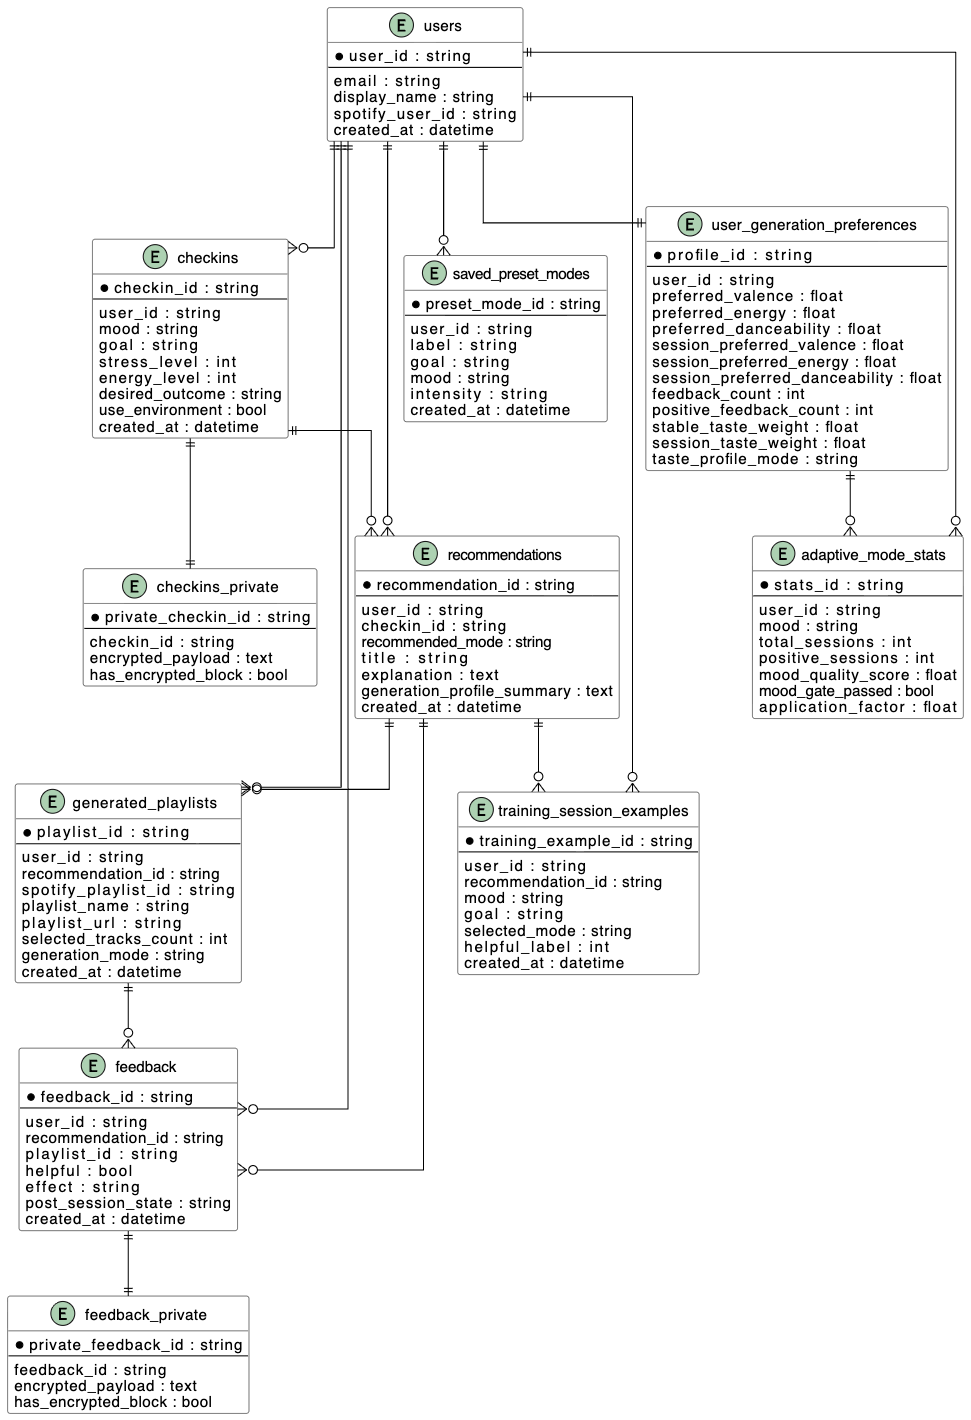
\includegraphics[width=0.78\linewidth]{Imagenes/diagrama_entidad_relacion.png}
    \caption{Diagrama entidad-relación lógico principal de Harmony Hub.}
    \label{fig:er_principal}
\end{figure}

\subsection{Colecciones y documentos principales}

\begin{center}
\captionsetup{type=table}
\scriptsize
\renewcommand{\arraystretch}{1.1}
\setlength{\tabcolsep}{3pt}
\begin{tabularx}{\textwidth}{|P{2.75cm}|P{1.9cm}|Y|P{1.9cm}|}
\hline
\textbf{Colección} & \textbf{ID doc.} & \textbf{Contenido representativo} & \textbf{Nivel} \\
\hline
\texttt{users} & UID del usuario & Perfil mínimo autenticado y referencia de identidad. & Alta \\
\hline
\texttt{checkins} & ID autogenerado & Bloque público mínimo del check-in: usuario, resumen del entorno acústico, densidad de muestreo, estabilidad, referencia al bloque privado y fecha. & Media \\
\hline
\shortstack[l]{\texttt{checkins\_}\\\texttt{private}} & Mismo ID del check-in & Bloque cifrado con estado de ánimo, objetivo, estrés, energía y resultado deseado. & Alta \\
\hline
\shortstack[l]{\texttt{recommendations}} & ID autogenerado & Título de recomendación, modo recomendado, targets musicales, origen de selección, estado de uso del entorno y contexto resumido. & Media \\
\hline
\shortstack[l]{\texttt{generated\_}\\\texttt{playlists}} & ID autogenerado & Identificador y URL de playlist, modo usado, número de pistas, pesos de aprendizaje aplicados y estado final del uso del entorno. & Media \\
\hline
\texttt{feedback} & ID autogenerado & Referencia a la recomendación, uso para aprendizaje, alcance de preferencia y bloque público mínimo. & Media \\
\hline
\shortstack[l]{\texttt{feedback\_}\\\texttt{private}} & Mismo ID del feedback & Valoración global, estado posterior de sesión y comentario cifrado. & Alta \\
\hline
\shortstack[l]{\texttt{saved\_preset\_}\\\texttt{modes}} & UID\_modo & Modo rápido guardado por el usuario y sus metadatos descriptivos. & Baja \\
\hline
\shortstack[l]{\texttt{user\_generation\_}\\\texttt{preferences}} & ID Spotify del usuario & Perfil aprendido agregado: preferencias de energía, valencia, ritmo, pesos estable/contextual y estadísticas específicas por mood. & Media \\
\hline
\shortstack[l]{\texttt{training\_session\_}\\\texttt{examples}} & UUID & Ejemplos agregados de sesión cerrada usados para entrenar y evaluar el modelo supervisado. & Media \\
\hline
\end{tabularx}
\caption{Colecciones principales de Firestore y tipo de información que almacenan.}
\label{tab:colecciones_firestore}
\end{center}

Esta organización muestra una decisión de diseño relevante: las unidades de uso
visibles para el usuario (check-in, recomendación, playlist y feedback) no se
guardan como un único documento gigante, sino como un conjunto trazable de
documentos enlazados. La separación entre bloques públicos mínimos y bloques
privados cifrados reduce exposición innecesaria y, además, mantiene claridad
sobre qué piezas necesita realmente cada parte de la aplicación.

También conviene distinguir dos niveles de agregación que en la interfaz pueden
parecer similares pero no cumplen la misma función. El documento de
preferencias de generación conserva el perfil visible del usuario y contadores
agregados de uso, mientras que la colección de ejemplos de entrenamiento a
nivel de sesión representa la base real utilizada para el modelo supervisado.
Esta separación resulta útil porque el perfil puede mostrar aprendizaje
acumulado y insights válidos aun cuando el clasificador global todavía
no dispone de balance suficiente para activarse.

En el estado actual del proyecto, esta diferencia ya se aprecia con claridad en
la práctica. El perfil visible del usuario longitudinal empleado para la
validación muestra actividad acumulada suficiente para sostener aprendizaje
individual estable, mientras que la base real del modelo supervisado de sesión
continúa condicionada por el balance entre ejemplos útiles y no útiles. Esta
asimetría no es un error de datos, sino la consecuencia de distinguir entre un
perfil agregado de uso visible y el subconjunto de sesiones realmente
consolidado para entrenamiento supervisado.

\section{Diseño funcional}
\label{sec:diseno_funcional}

Desde el punto de vista funcional, la solución se apoya en varios módulos que
cooperan entre sí: autenticación, gestión de sesión con Spotify, captura del
entorno, recomendación, persistencia de historial, gestión del feedback y modos
rápidos.

La \textbf{Figura~\ref{fig:clases_general}} resume esta organización interna a
través de un diagrama de clases general. En él se aprecia cómo la aplicación se
articula alrededor de servicios, modelos y componentes de persistencia
especializados, en lugar de concentrar demasiada lógica en una sola capa.

Además, para comprender bien el comportamiento dinámico del sistema, conviene
observar cómo se encadena el flujo completo de una sesión musical. La
\textbf{Figura~\ref{fig:actividades_sesion}} resume primero esa lógica desde un
punto de vista de actividades y decisiones. A continuación, la
\textbf{Figura~\ref{fig:secuencia_principal}} representa la secuencia principal
desde la interacción inicial del usuario hasta la creación de la playlist y el
registro del feedback posterior.

Este bloque funcional puede leerse desde tres perspectivas complementarias. La
vista de clases ayuda a entender qué piezas cooperan entre sí; la vista de
actividades muestra en qué orden se activan las decisiones principales; y la
vista de secuencia deja ver cómo circulan las llamadas entre cliente, backend,
motor híbrido y servicios externos durante una sesión real.

Por último, el cierre del ciclo se detalla en la
\textbf{Figura~\ref{fig:secuencia_feedback}}, donde se aprecia cómo el feedback
del usuario no solo se almacena, sino que desencadena la actualización del
perfil individual, la conservación de ejemplos supervisados y la auditoría del
estado del modelo.

\begin{landscape}
\begin{figure}[p]
    \centering
    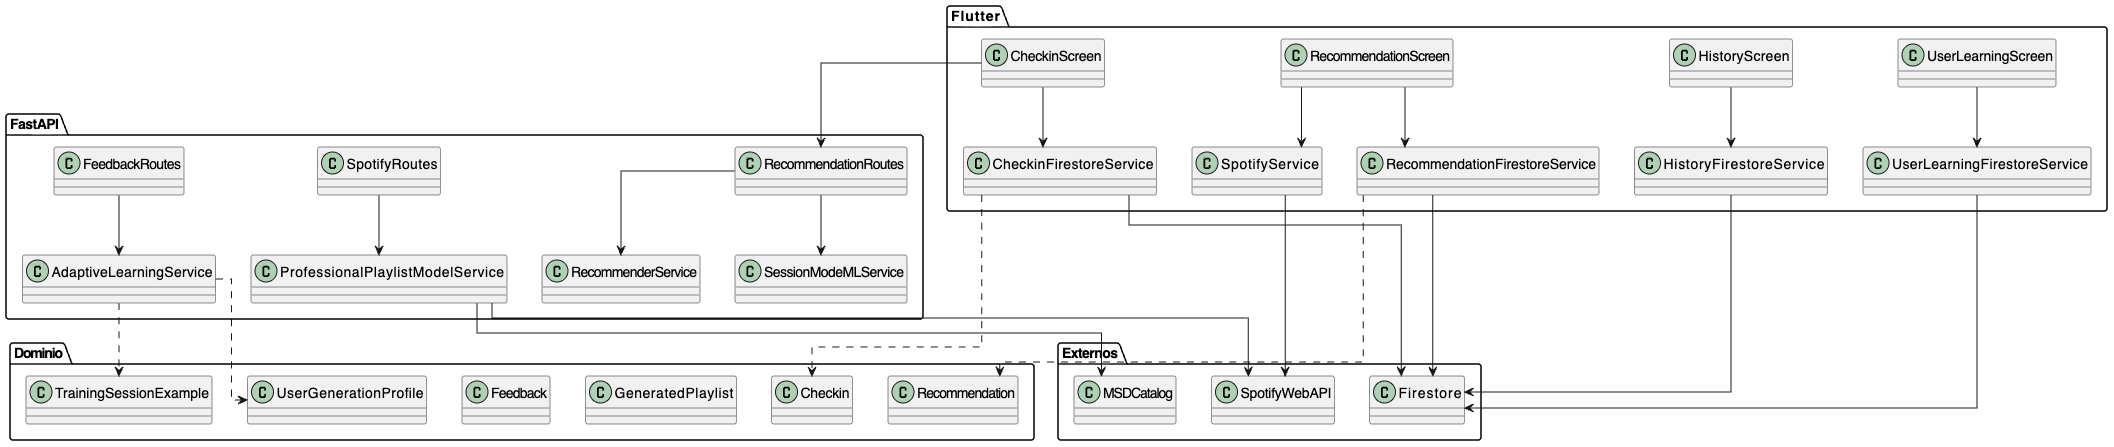
\includegraphics[width=\linewidth,height=0.84\textheight,keepaspectratio]{Imagenes/diagrama_clases_general.png}
    \caption{Diagrama de clases general de Harmony Hub.}
    \label{fig:clases_general}
\end{figure}
\end{landscape}

La vista de actividades permite leer el flujo desde una perspectiva menos
estructural y más operativa. En ella se distinguen con claridad tres momentos:
la recogida del contexto inicial mediante el check-in y, en su caso, el
entorno acústico; la generación y materialización de la sesión musical; y el
cierre del ciclo por medio del feedback, que activa tanto la actualización del
perfil aprendido como la consolidación de nuevos ejemplos supervisados. La
representación también resulta útil para mostrar que ciertos pasos son
condicionales, como la medición del entorno, la solicitud de playlist o el
envío de feedback posterior.

\begin{figure}[H]
    \centering
    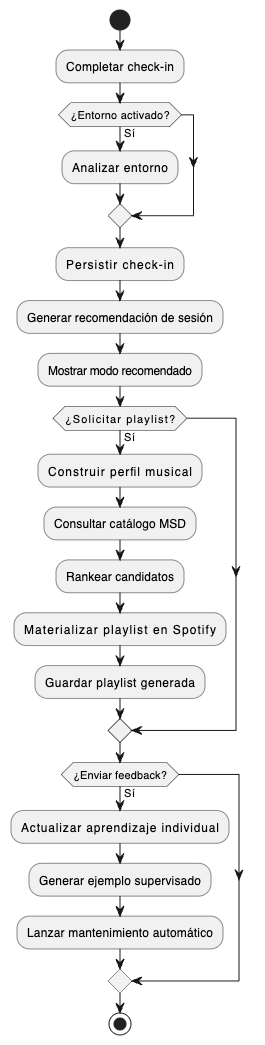
\includegraphics[width=0.38\textwidth,height=0.56\textheight,keepaspectratio]{Imagenes/diagrama_actividades_sesion.png}
    \caption{Diagrama de actividades del flujo principal de generación de sesión musical.}
    \label{fig:actividades_sesion}
\end{figure}

\begin{landscape}
\begin{figure}[p]
    \centering
    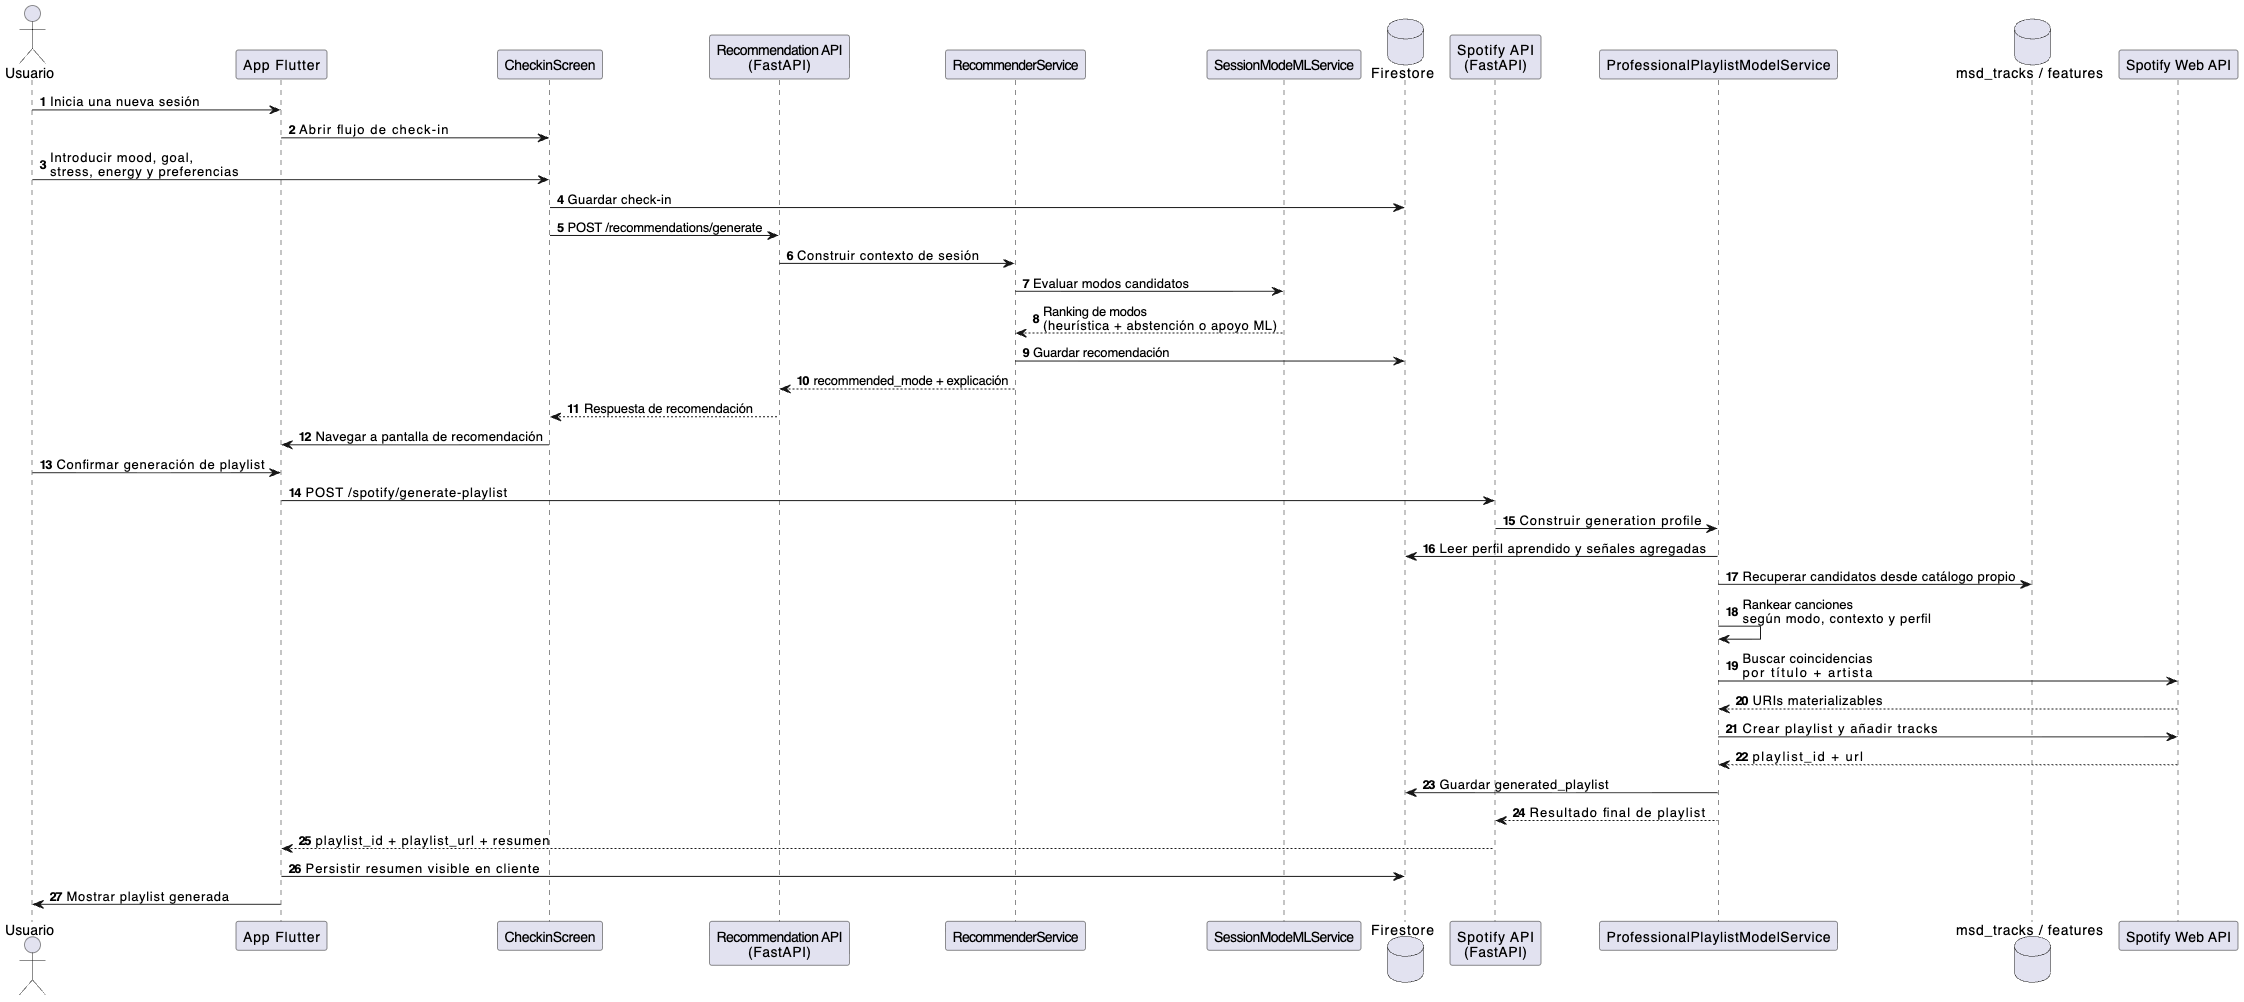
\includegraphics[width=\linewidth,height=0.84\textheight,keepaspectratio]{Imagenes/diagrama_secuencia_principal.png}
    \caption{Diagrama de secuencia principal del flujo de generación de sesión musical.}
    \label{fig:secuencia_principal}
\end{figure}
\end{landscape}

Ese flujo general se complementa con una vista más específica del tratamiento
del feedback. La \textbf{Figura~\ref{fig:secuencia_feedback}} muestra cómo el
backend utiliza esa valoración para actualizar estadísticas, conservar ejemplos
de entrenamiento y, además, separar el feedback público de la parte sensible
cifrada antes de persistirlo en Firestore.

\begin{landscape}
\begin{figure}[p]
    \centering
    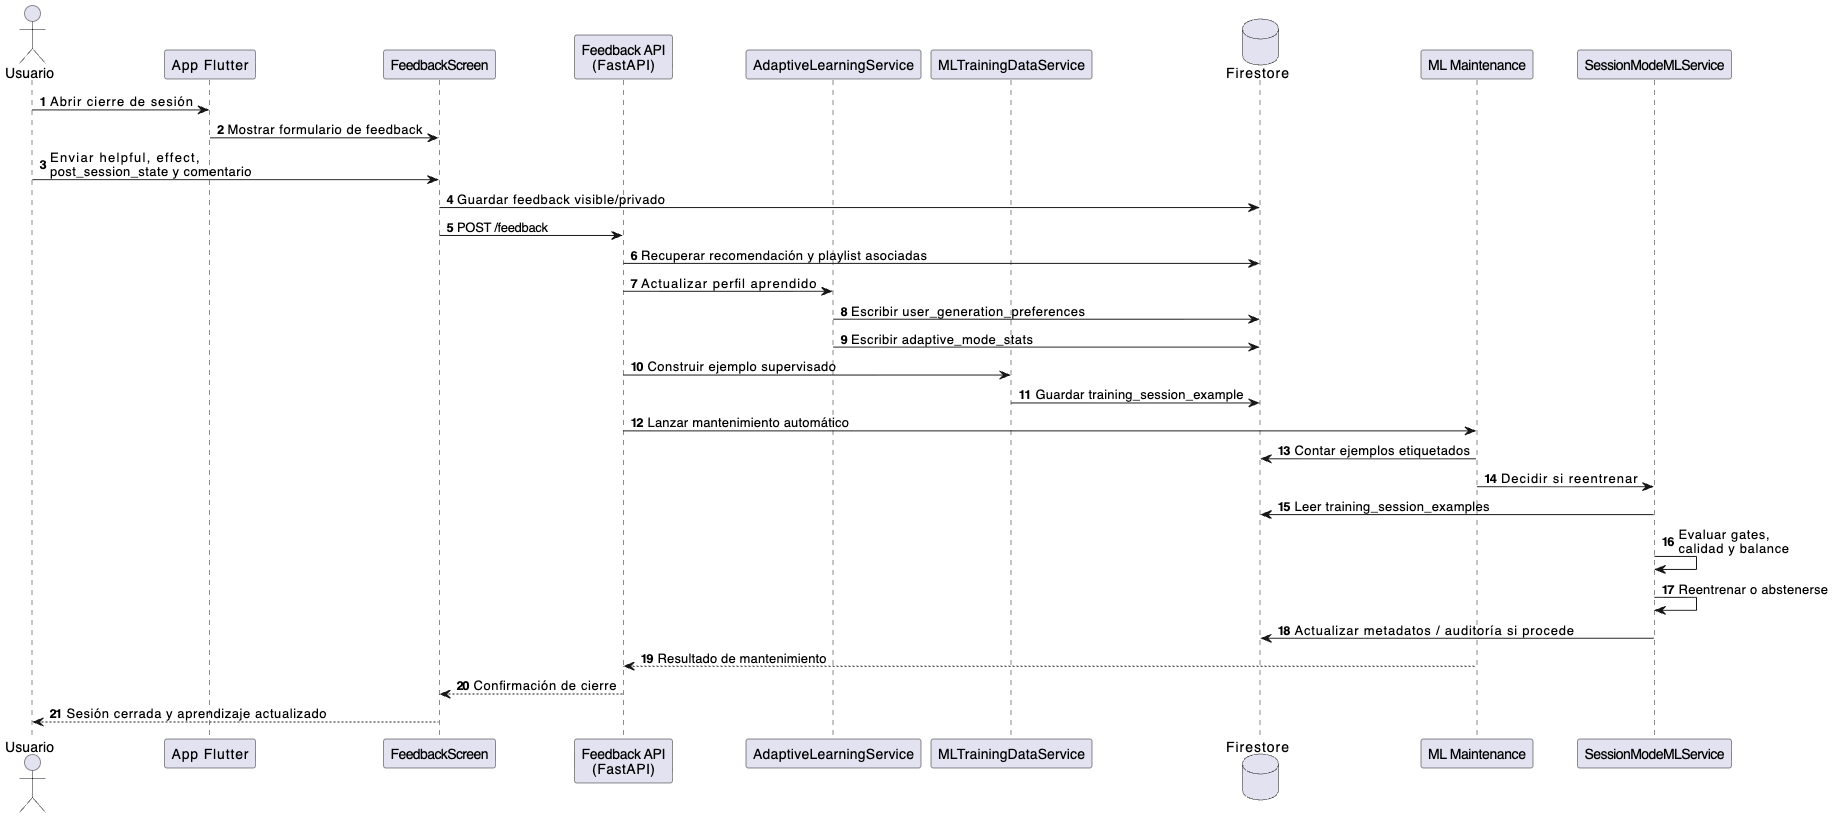
\includegraphics[width=0.92\linewidth,height=0.8\textheight,keepaspectratio]{Imagenes/diagrama_secuencia_feedback.png}
    \caption{Diagrama de secuencia específico del proceso de feedback y actualización del aprendizaje.}
    \label{fig:secuencia_feedback}
\end{figure}
\end{landscape}

La lógica operativa de este cierre puede resumirse en un pseudocódigo breve, en
el que se observa cómo el feedback no solo registra la valoración de la sesión,
sino que desencadena la actualización del perfil individual y la consolidación
de nuevos ejemplos para el modelo supervisado.

\begin{listing}[H]
\begin{minted}[fontsize=\small,breaklines]{text}
ALGORITMO CerrarSesionConFeedback(feedback, recomendacion, playlist)
  guardar bloque publico y bloque privado del feedback
  recuperar contexto de recomendacion y playlist asociada

  actualizar perfil aprendido del usuario
  actualizar estadisticas agregadas por mood

  construir ejemplo supervisado de sesion cerrada
  guardar ejemplo en la coleccion de entrenamiento

  ejecutar mantenimiento automatico del modelo
  SI el reentrenado supera puertas de datos y calidad ENTONCES
    actualizar artefactos y metadatos del modelo
  SI NO
    mantener abstencion conservadora
  FIN SI
FIN ALGORITMO
\end{minted}
\caption{Pseudocódigo del cierre de sesión con feedback y actualización del aprendizaje.}
\label{lst:pseudocodigo_feedback}
\end{listing}

Si se sigue el mismo hilo que aparece en el diagrama general de casos de uso,
el diseño funcional puede entenderse como una cadena de bloques que se apoyan
entre sí y que, poco a poco, van cerrando el ciclo completo de uso.

\subsection{Acceso y recuperación de cuenta}

El primer bloque cubre el alta del usuario, el inicio de sesión y la
recuperación de contraseña. Aunque pueda parecer una parte más convencional del
proyecto, aquí ya aparecen dos necesidades importantes: reducir fricción de
entrada y asegurar que la experiencia no se rompa cuando el usuario pierde el
acceso a la cuenta. Por eso se optó por una autenticación basada en Firebase,
con persistencia mínima del perfil y un mecanismo de restablecimiento que se
apoya en el correo real asociado a la cuenta.

\subsection{Check-in y generación de recomendación}

El núcleo de Harmony Hub empieza realmente en el check-in. Esta parte está
pensada para capturar el estado del usuario sin convertir la interacción en un
formulario pesado. Se recogen variables como estado de ánimo, objetivo, nivel
de energía, nivel de estrés y, cuando procede, contexto acústico del entorno.

Después, el backend traduce ese contexto en una recomendación de sesión. Aquí
la intención no es decirle al usuario ``qué canción debería escuchar'', sino
darle una propuesta funcional de sesión con sentido para ese momento concreto.
Además, cada recomendación queda vinculada a un identificador que sirve como
hilo conductor del resto del flujo.

\subsection{Conexión con Spotify y materialización de la sesión}

La recomendación, por sí sola, todavía no resuelve el problema. Tiene que
convertirse en una playlist real y reproducible dentro de una plataforma de uso
cotidiano. Para eso se integra Spotify mediante OAuth y un backend intermedio
que gestiona tanto el intercambio de credenciales como la creación posterior de
la playlist.

Este bloque tiene bastante peso arquitectónico, porque conecta el dominio
propio de Harmony Hub con un servicio externo sobre el que la aplicación no
tiene control absoluto. Y es precisamente ahí donde cobra sentido haber
separado interfaz, backend y persistencia.

\subsection{Historial y memoria de uso}

Una vez generadas varias sesiones, la aplicación necesita ofrecer al usuario un
espacio donde recuperar lo vivido. El historial no se plantea solo como una
lista de eventos técnicos, sino como una memoria funcional de check-ins,
recomendaciones, playlists y valoraciones. Esto permite volver sobre sesiones
anteriores, reinterpretar patrones y reforzar la sensación de continuidad entre
usos.

\subsection{Modos rápidos}

Los modos rápidos responden a una idea bastante simple, pero muy útil: hay
situaciones que se repiten. Por eso el sistema ofrece accesos predefinidos para
momentos como entrar en foco, bajar carga mental o cambiar de ritmo tras una
jornada intensa. Desde el diseño funcional, esta capa actúa como un atajo
práctico entre el uso libre y el uso recurrente.

\subsection{Feedback y aprendizaje personal}

El cierre del flujo llega con el feedback. Cuando el usuario valora si la
sesión le ayudó, la aplicación no solo guarda una respuesta; convierte esa
valoración en evidencia para entender mejor qué propuestas funcionan y cuáles
no. Además, este diseño se ha construido con una separación entre bloque
público y bloque privado cifrado, algo que refuerza la seguridad de información
sensible como comentarios o estados posteriores de sesión.

Por encima de ese feedback puntual aparece el aprendizaje personal, que no se
presenta como una inteligencia mágica ni como una caja negra opaca. Se apoya en
estadísticas acumuladas, trazabilidad entre recomendación y resultado, y una
aplicación prudente de pesos aprendidos. En la implementación actual esto se traduce en
modos operativos como \texttt{progressive\_contextual} o
\texttt{stable\_weighted}, que permiten explicar cuándo el sistema usa memoria
estable, cuándo aplica solo una parte de lo aprendido y cuándo todavía depende
principalmente del contexto inmediato.

En la práctica, esta capa es también la que alimenta la pantalla de aprendizaje
visible para el usuario. Los insights sobre tono emocional, energía o
ritmo habitual se derivan del documento agregado del perfil, no del artefacto
del modelo supervisado. Esto mejora la explicabilidad del producto final,
porque permite enseñar aprendizaje útil incluso cuando el clasificador global
todavía no ha alcanzado madurez suficiente.

Conviene precisar cómo decide el sistema si una sesión debe apoyarse más en el
perfil reciente o en el perfil estable. En la implementación actual se calculan
dos pesos continuos: un peso de sesión, asociado a la evidencia contextual o
de corto plazo, y un peso estable, asociado al histórico más consolidado del
usuario. Ambos pesos no se fijan manualmente, sino que dependen de la
consistencia observada en el feedback positivo y negativo acumulado. Cuando el
peso estable supera al peso de sesión, el modo interno del perfil pasa a
\texttt{stable\_weighted}; cuando ocurre lo contrario, el sistema utiliza
\texttt{session\_weighted}. Si la evidencia del mood actual todavía no es
suficiente para aplicar el aprendizaje completo, aparece un estado intermedio,
\texttt{progressive\_contextual}, que mantiene una aplicación parcial y más
prudente.

Este reparto se normaliza reservando una masa base unitaria para el contexto
actual de la sesión. La decisión no es arbitraria: sirve para garantizar que
el aprendizaje previo no sustituya el check-in presente, sino que actúe como
factor de corrección progresiva. En otras palabras, el sistema preserva un
espacio fijo para lo que el usuario declara y vive en ese momento —objetivo,
estado emocional, nivel de energía, estrés, resultado deseado y entorno—, y
solo después distribuye el peso adicional entre memoria de sesión y memoria
estable según la evidencia observada. Gracias a esta masa base, Harmony Hub
aprende sin encasillar y mantiene la capacidad de responder principalmente a la
necesidad del momento.

El efecto real de esta decisión no consiste en sustituir el check-in por el
histórico, sino en desplazar progresivamente los valores objetivo de la
sesión. Por ejemplo, si el contexto actual sugiere una energía base de 0.50,
el aprendizaje reciente de sesión apunta a 0.44 y el perfil estable indica que
históricamente suele funcionar mejor una energía próxima a 0.38, el sistema no
salta directamente al valor estable. Primero mezcla el valor base con el valor
de sesión según su peso contextual y, después, vuelve a mezclar el resultado
con el valor estable. Si, por ejemplo, el peso de sesión es 0.17 y el peso
estable es 0.28, el valor final de energía queda aproximadamente en 0.46. Esto
permite conservar la señal del momento actual, pero corrigiéndola de forma
gradual hacia lo que el histórico del usuario ha demostrado que suele
funcionarle mejor. La misma lógica se aplica también a los valores objetivo de
valencia y bailabilidad, por lo que la diferencia entre un perfil más estable y
uno más contextual se traduce en ajustes musicales reales, no solo en una
etiqueta mostrada en pantalla.

La Tabla~\ref{tab:modos_perfil_aprendizaje} resume de forma comparativa estos
cuatro estados internos del perfil aprendido y su efecto práctico sobre la
sesión.

\begin{table}[H]
\centering
\small
\renewcommand{\arraystretch}{1.12}
\begin{tabularx}{\textwidth}{|P{2.9cm}|P{3.1cm}|Y|}
\hline
\textbf{Modo interno} & \textbf{Condición principal} & \textbf{Interpretación funcional} \\
\hline
\texttt{\seqsplit{context\_only}} & La suma de pesos aprendidos es prácticamente nula. & El sistema trabaja casi exclusivamente con el check-in actual. Todavía no existe evidencia suficiente como para que el aprendizaje previo modifique de forma apreciable los targets musicales. \\
\hline
\texttt{\seqsplit{progressive\_contextual}} & El mood actual aún no ha superado su umbral de madurez local, pero ya existe cierta evidencia parcial. & Se aplica una parte del aprendizaje acumulado de forma prudente. El sistema no ignora el histórico, pero evita dejar que domine mientras la evidencia específica del mood siga siendo insuficiente. \\
\hline
\texttt{\seqsplit{session\_weighted}} & El peso de sesión es mayor o igual que el peso estable. & La sesión se corrige principalmente con señales recientes o más contextuales. Esto suele ocurrir cuando el patrón observado en sesiones próximas resulta más informativo que el histórico general. \\
\hline
\texttt{\seqsplit{stable\_weighted}} & El peso estable supera al peso de sesión. & La corrección principal proviene del perfil histórico consolidado. El sistema sigue partiendo del check-in actual, pero desplaza con más fuerza los targets hacia aquello que ha demostrado funcionar mejor de forma recurrente para el usuario. \\
\hline
\end{tabularx}
\caption{Estados internos del perfil aprendido y su efecto sobre la personalización musical.}
\label{tab:modos_perfil_aprendizaje}
\end{table}

\section{Diseño de la interfaz}
\label{sec:diseno_interfaz}

La interfaz se diseñó con una idea bastante clara desde el principio: la app
debía sentirse íntima, ligera y guiada, no como una herramienta técnica que
obliga al usuario a pensar demasiado antes de poder usarla. Y es que, si el
objetivo del sistema es ayudar a regular un momento interno, una interfaz fría
o excesivamente mecánica jugaría en contra de esa intención.

En términos de navegación, la aplicación se estructura alrededor de una barra
inferior con accesos a los apartados principales: inicio, modos, historial,
aprendizaje y perfil. Esta organización busca que el usuario tenga siempre una
idea bastante clara de dónde está y qué puede hacer a continuación.

La Figura~\ref{fig:diagrama_navegacion_app} resume este recorrido de manera
global. En ella se observa tanto el acceso inicial mediante autenticación y
conexión con Spotify como la navegación principal dentro del \textit{AppShell},
desde donde se articula el flujo más importante del sistema: check-in,
recomendación, generación de playlist y devolución de feedback.

\begin{figure}[htbp]
\centering
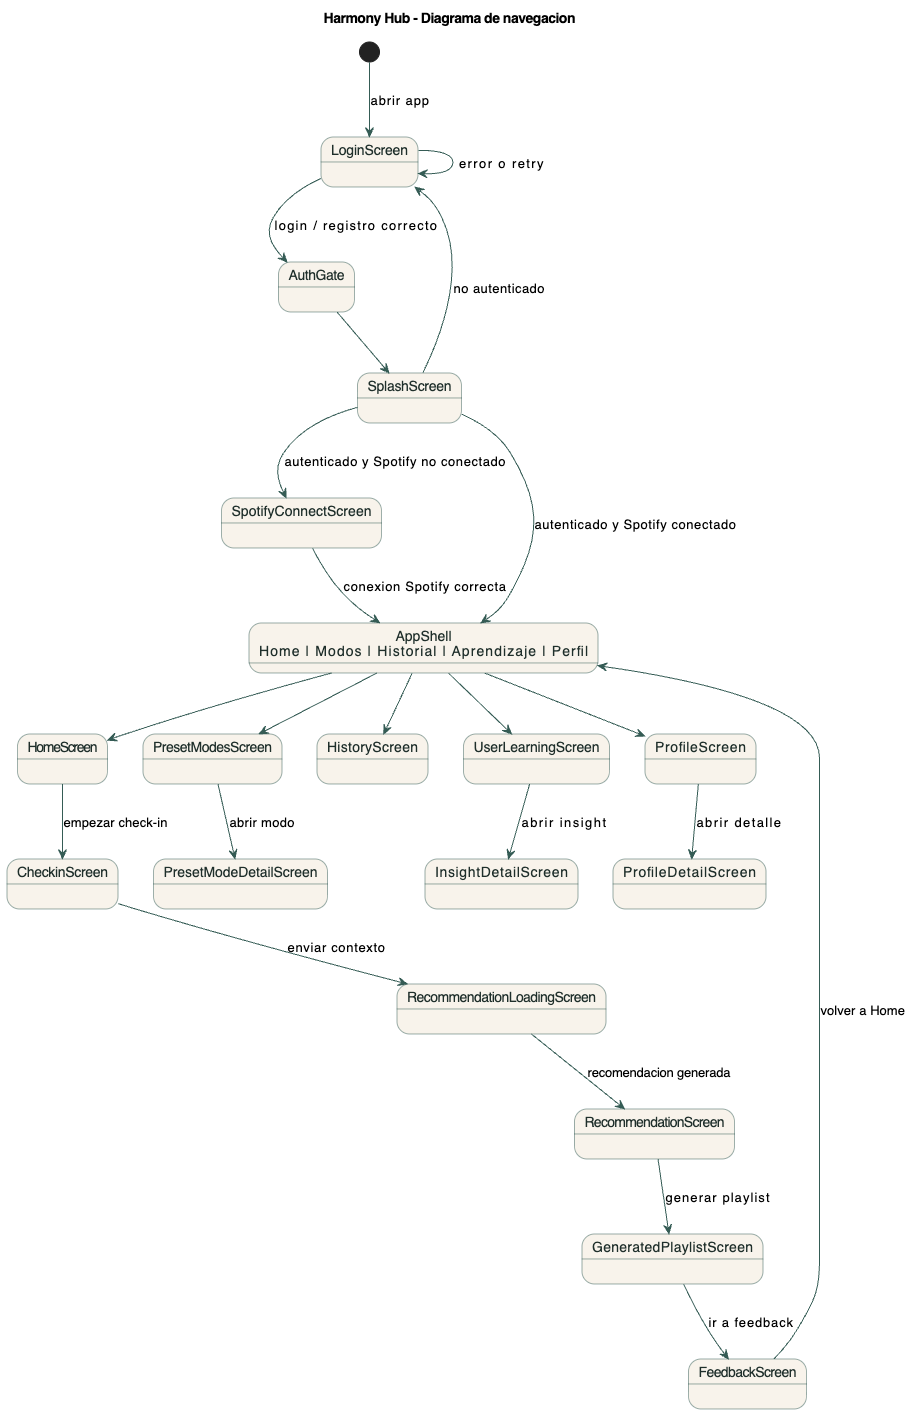
\includegraphics[width=0.72\textwidth]{Imagenes/diagrama_navegacion_app.png}
\caption{Diagrama de navegación principal de Harmony Hub.}
\label{fig:diagrama_navegacion_app}
\end{figure}

Para complementar esa visión estructural, resulta útil mostrar también algunas
pantallas clave del producto final. La Figura~\ref{fig:interfaz_principal_app}
reúne cuatro momentos representativos del flujo: acceso inicial, pantalla
principal, recomendación contextual y playlist generada. Esta selección permite
ver cómo la lógica funcional del sistema se traduce en una interfaz móvil
coherente y suficientemente guiada.

\begin{figure}[htbp]
\centering
\begin{minipage}{0.23\textwidth}
    \centering
    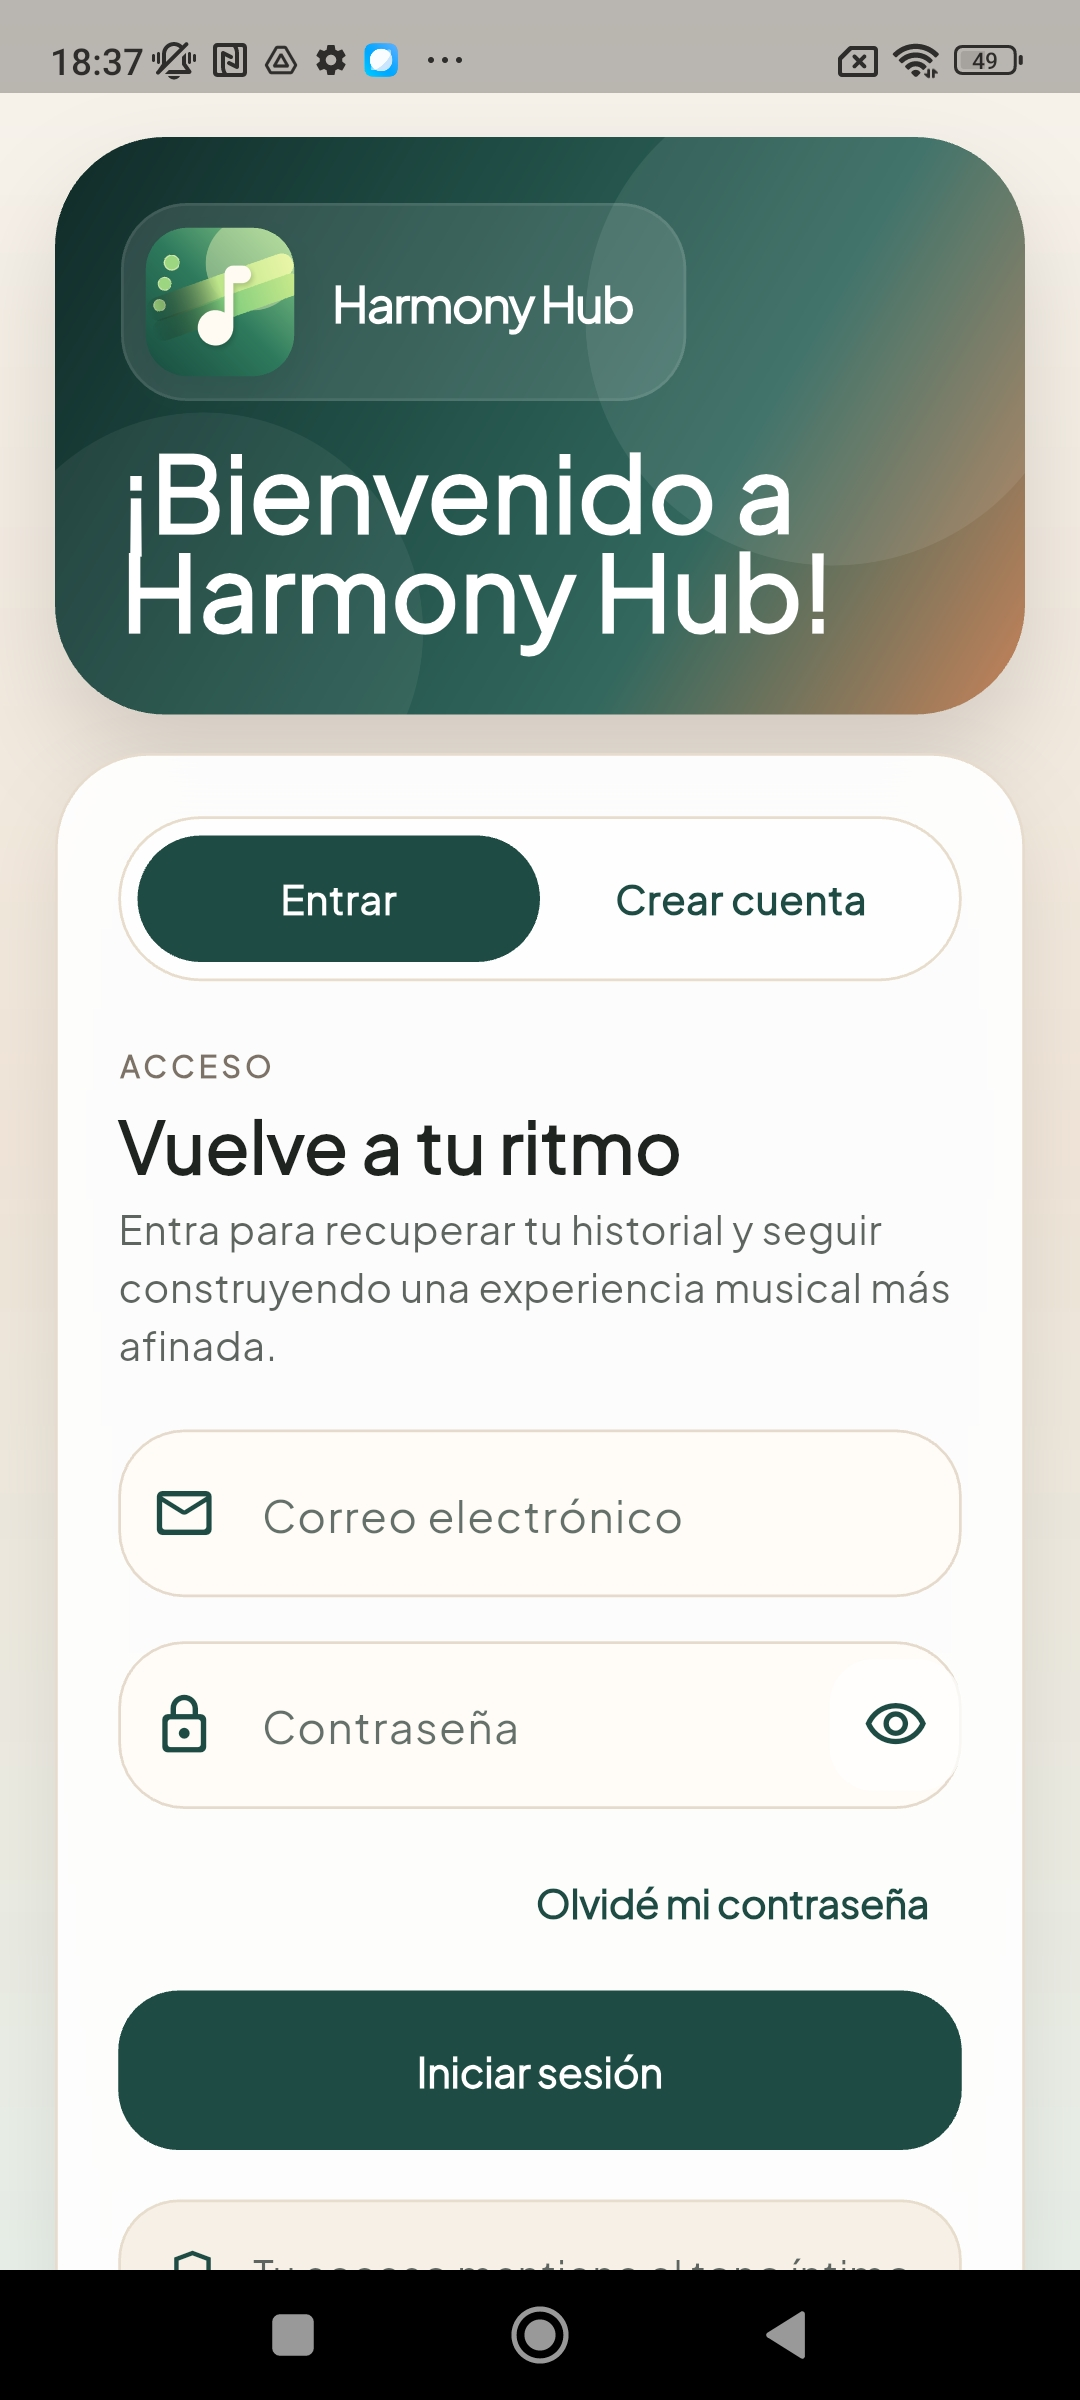
\includegraphics[width=\linewidth]{Imagenes/manual_app/Screenshot_2026-05-25-18-37-08-051_com.example.harmonyhub.jpg}
\end{minipage}
\hfill
\begin{minipage}{0.23\textwidth}
    \centering
    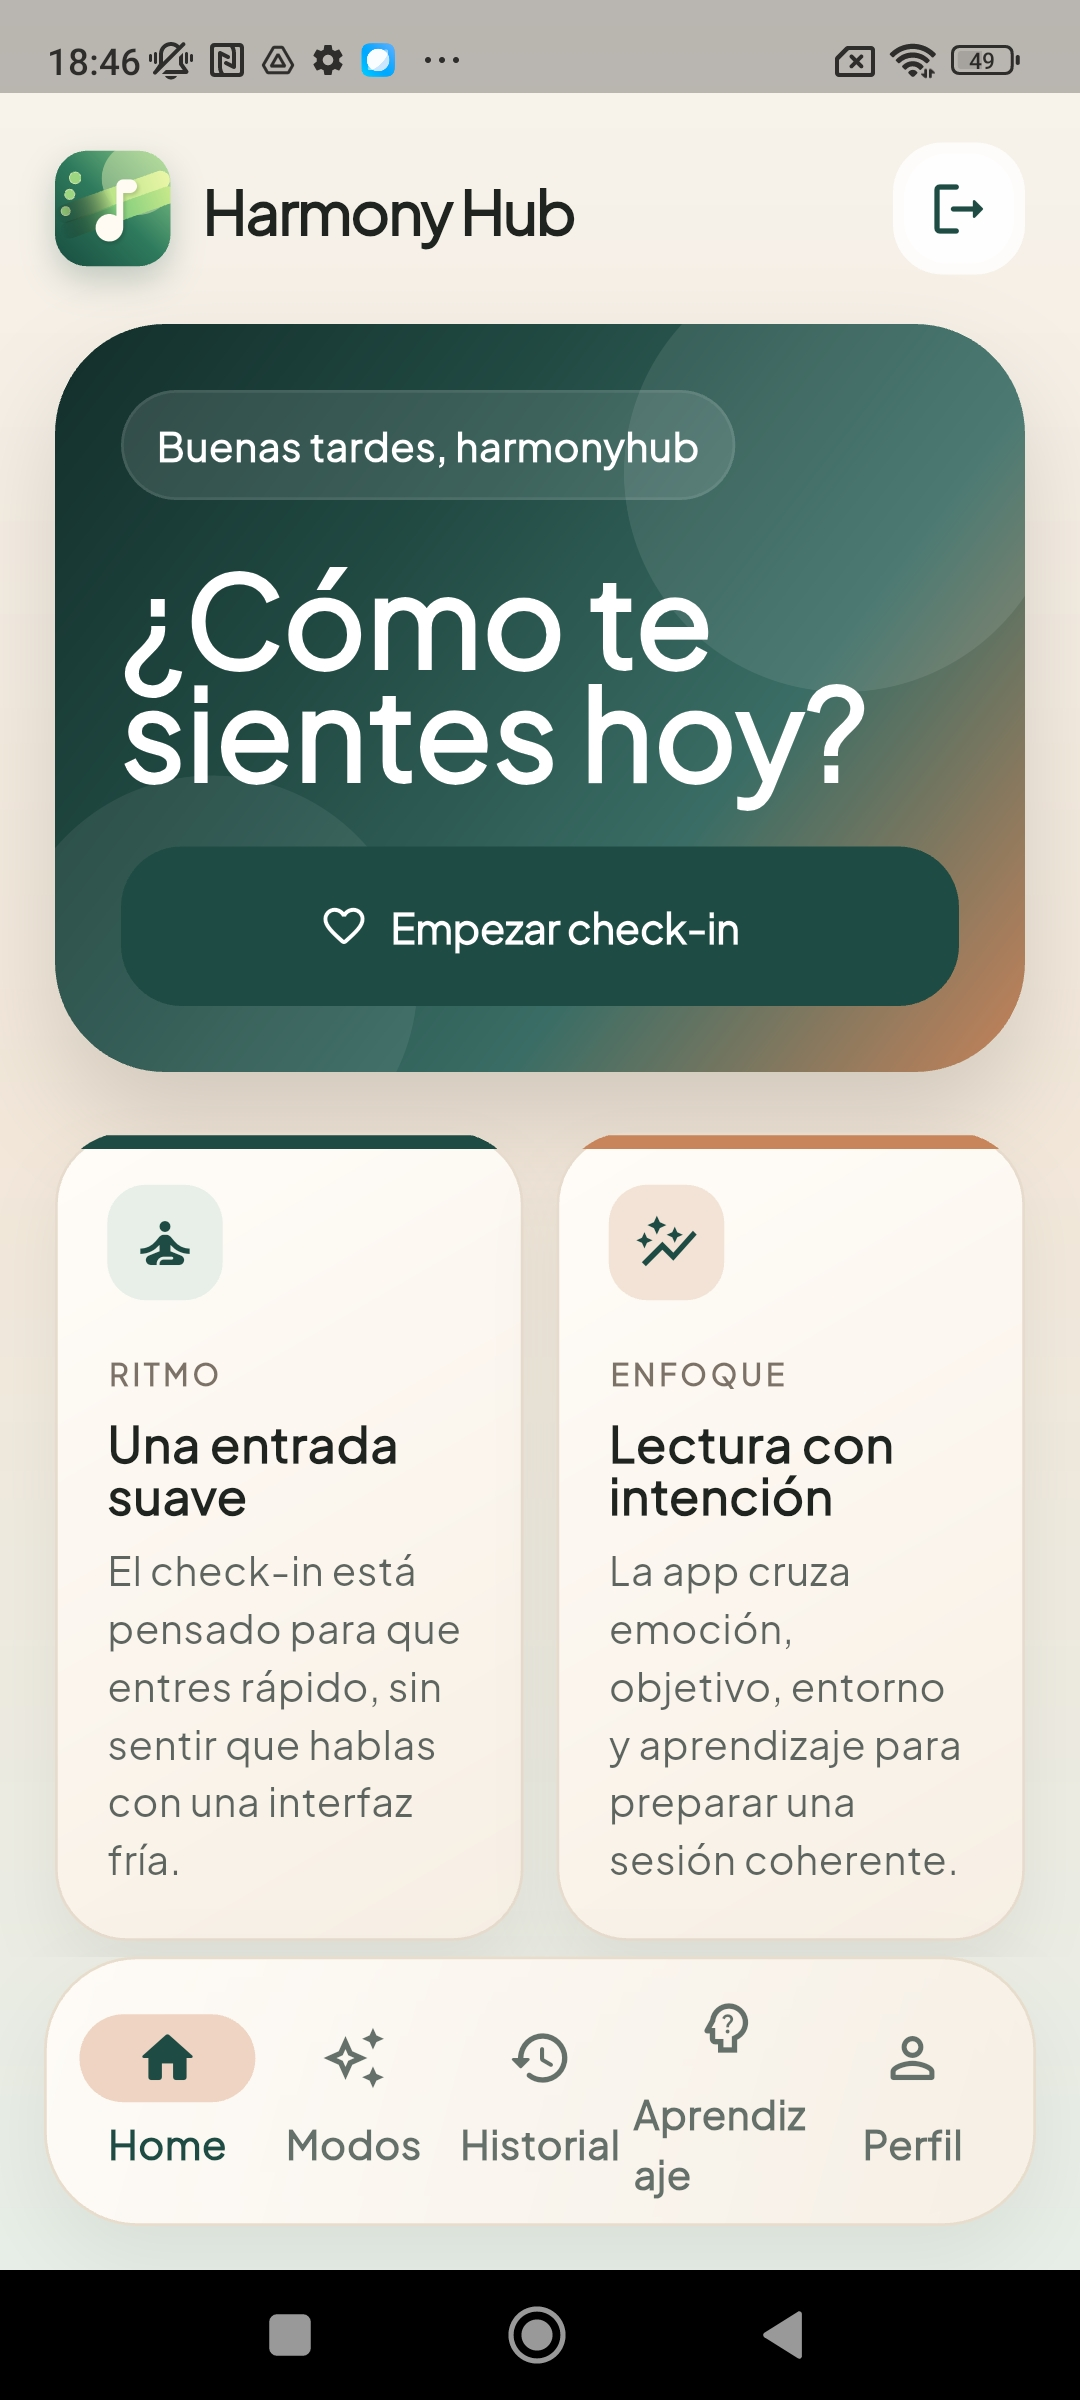
\includegraphics[width=\linewidth]{Imagenes/manual_app/Screenshot_2026-05-25-18-46-14-698_com.example.harmonyhub.jpg}
\end{minipage}
\hfill
\begin{minipage}{0.23\textwidth}
    \centering
    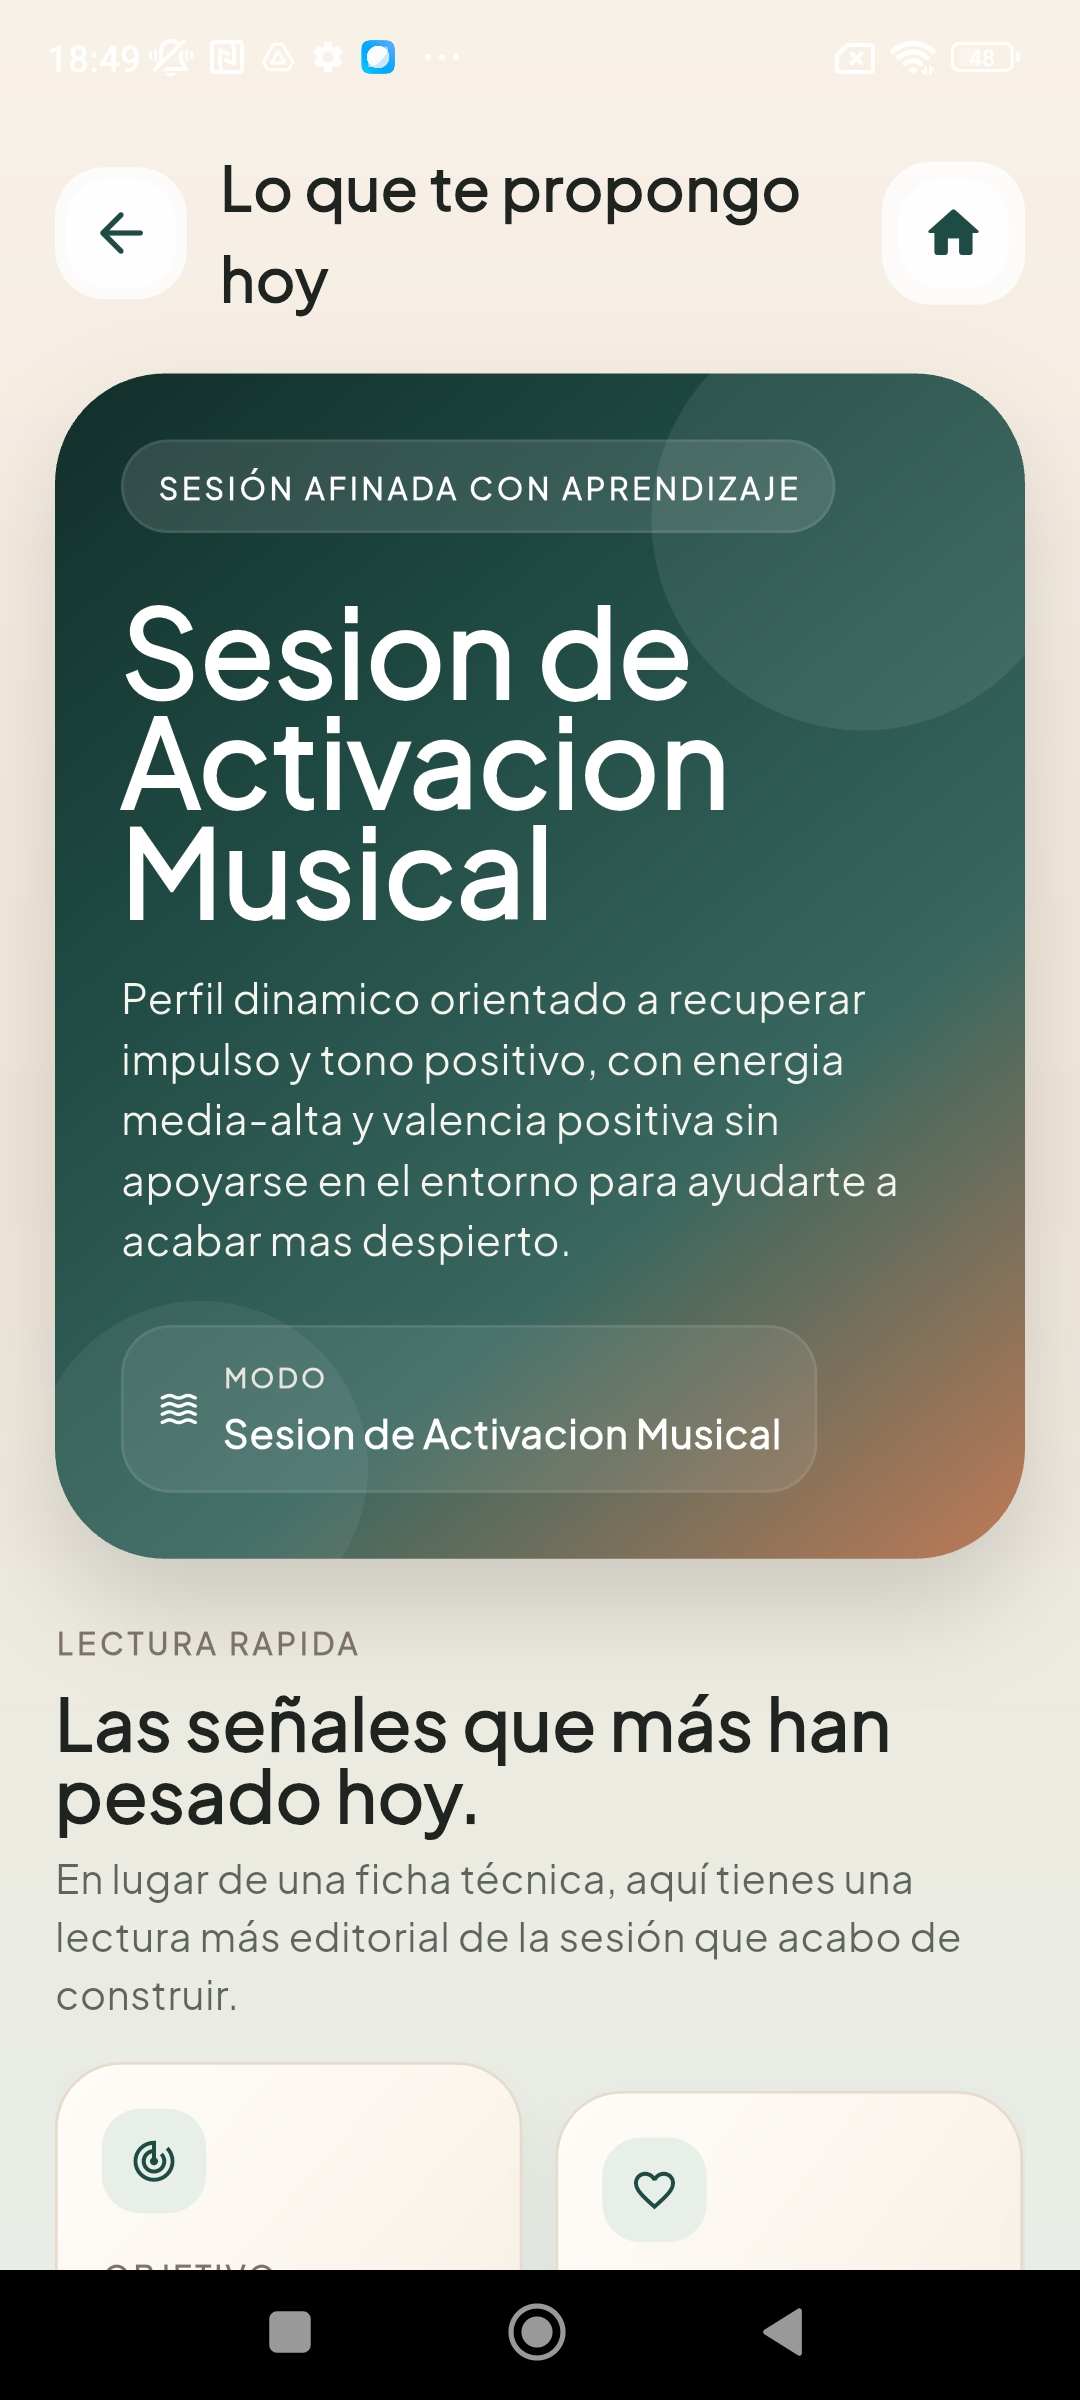
\includegraphics[width=\linewidth]{Imagenes/manual_app/Screenshot_2026-05-25-18-49-39-980_com.example.harmonyhub.jpg}
\end{minipage}
\hfill
\begin{minipage}{0.23\textwidth}
    \centering
    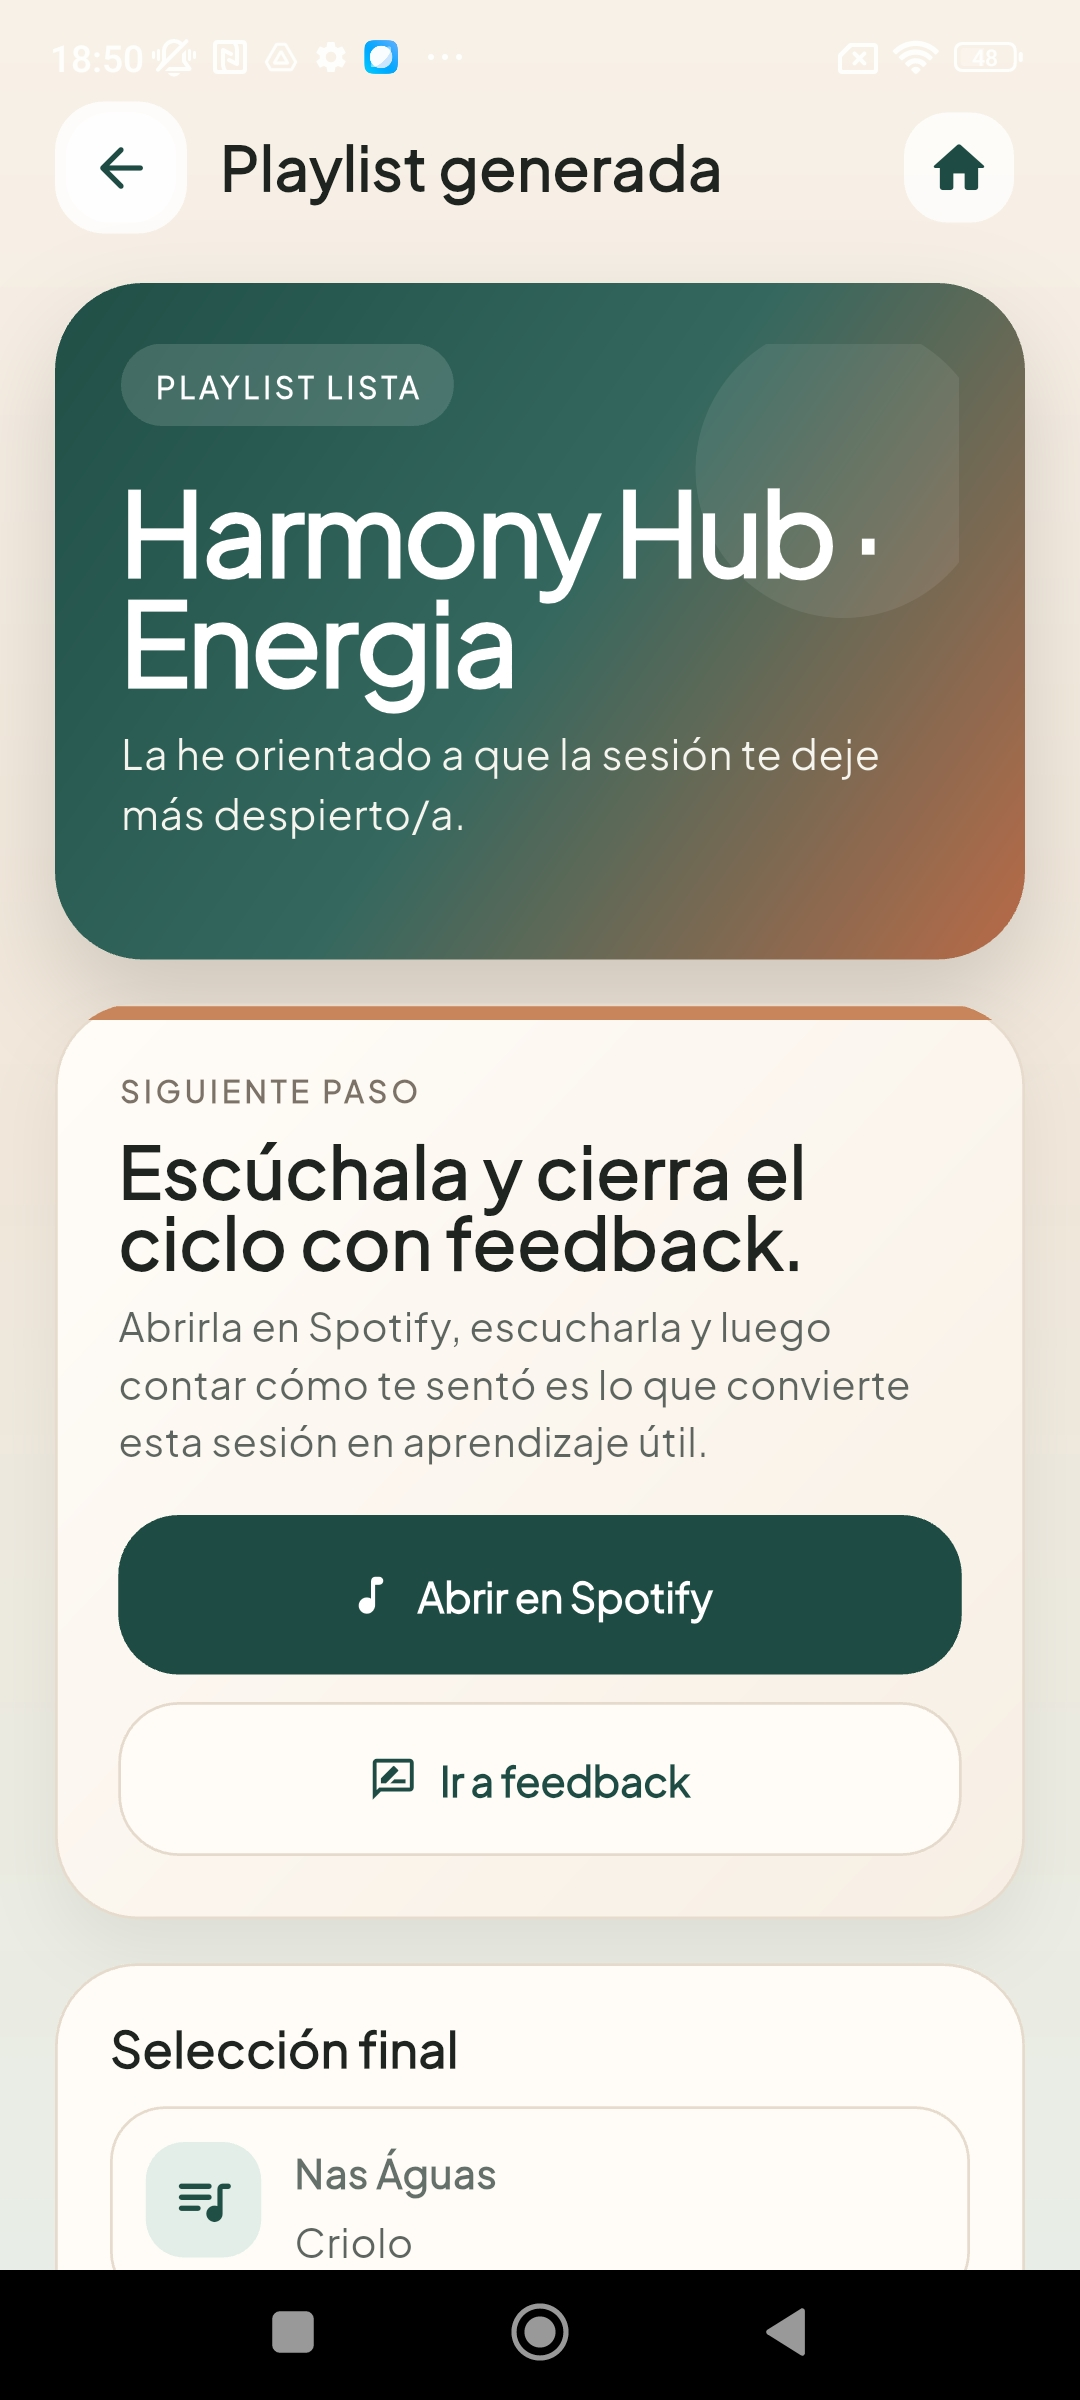
\includegraphics[width=\linewidth]{Imagenes/manual_app/Screenshot_2026-05-25-18-50-27-942_com.example.harmonyhub.jpg}
\end{minipage}
\caption{Pantallas representativas de la interfaz final: acceso, inicio, recomendación y playlist generada.}
\label{fig:interfaz_principal_app}
\end{figure}

Estas capturas permiten identificar cuatro decisiones de diseño. En primer
lugar, el acceso utiliza una jerarquía visual suave y directa, evitando
sobrecargar la pantalla inicial. En segundo lugar, la pantalla principal
prioriza la acción inmediata de comenzar una nueva sesión, lo que refuerza la
naturaleza cotidiana del uso. En tercer lugar, la recomendación no se presenta
como una simple lista de canciones, sino como una explicación funcional del
tipo de sesión propuesto. Por último, la materialización de la playlist deja
una sensación clara de cierre del flujo, ya que transforma la recomendación en
un recurso reproducible dentro de Spotify.

Desde el punto de vista visual, predominan bloques amplios, esquinas redondeadas,
colores suaves y una jerarquía tipográfica marcada, sobre todo en las pantallas
de acceso, home, Spotify Connect y feedback. No se trata solo de una decisión
estética: ese lenguaje visual ayuda a reducir saturación y refuerza la idea de
acompañamiento en lugar de exigir una interacción áspera o demasiado funcional.

También se tomaron decisiones específicas para mejorar la experiencia en móvil:

\begin{table}[H]
\centering
\small
\renewcommand{\arraystretch}{1.1}
\begin{tabularx}{\textwidth}{|P{4.4cm}|Y|}
\hline
\textbf{Decisión de interfaz} & \textbf{Justificación} \\
\hline
Jerarquía tipográfica muy marcada en pantallas clave & Permite que el usuario entienda rápidamente dónde está y cuál es la siguiente acción importante sin leer bloques largos. \\
\hline
Check-in guiado por pasos cortos & Reduce la sensación de cuestionario y favorece respuestas rápidas en momentos de carga mental o poco tiempo disponible. \\
\hline
CTA principal único por pantalla & Evita competencia entre acciones y refuerza la continuidad del flujo: entrar, responder, preparar playlist, escuchar y dar feedback. \\
\hline
Barra inferior estable para navegación principal & Mantiene orientación constante entre Home, Modos, Historial, Aprendizaje y Perfil, evitando menús escondidos o recorridos ambiguos. \\
\hline
Uso de tarjetas amplias y bloques redondeados & Favorece una percepción más suave y cercana, coherente con el propósito de bienestar cotidiano de la aplicación. \\
\hline
Reducción de densidad textual y agrupación por contexto & Facilita el escaneo rápido y evita saturar la pantalla con explicaciones técnicas o datos redundantes. \\
\hline
Revisión explícita de espaciados y overflows & Resulta necesaria para que la experiencia sea sólida también en dispositivos compactos y no se rompa en momentos críticos del flujo. \\
\hline
Presencia de branding propio y lenguaje visual coherente & Refuerza identidad de producto y ayuda a que Harmony Hub no se perciba como una demo técnica sin personalidad. \\
\hline
\end{tabularx}
\caption{Decisiones específicas adoptadas en el diseño de la interfaz.}
\label{tab:decisiones_interfaz}
\end{table}

\section{Diseño de pruebas}
\label{sec:diseno_pruebas}

El diseño de pruebas se planteó desde una lógica bastante práctica: no bastaba
con comprobar que la app ``abre'' o que una pantalla ``se ve''. Había que
validar el flujo completo, desde el acceso hasta la creación de la playlist y
el almacenamiento del feedback, sin perder de vista el comportamiento del
backend ni la dependencia de servicios externos.

Por eso, las pruebas se estructuran en varios niveles:

\begin{itemize}
    \item pruebas funcionales del flujo principal, centradas en autenticación, check-in, recomendación, playlist, historial y feedback;
    \item pruebas de integración, especialmente en la comunicación entre Flutter, FastAPI, Spotify y Firestore;
    \item pruebas de robustez frente a errores externos, como restricciones o respuestas inesperadas de Spotify;
    \item pruebas de consistencia del aprendizaje, verificando que la información necesaria queda registrada y que el modelo solo se activa con suficiente evidencia;
    \item pruebas de interfaz y usabilidad básica en móvil, incluyendo revisión de overflows, jerarquía visual y continuidad del flujo.
\end{itemize}

Los criterios de aceptación se apoyan en una idea sencilla: cada sesión debe
ser trazable de principio a fin, el sistema debe poder degradarse con dignidad
si falla una parte externa, y la experiencia no debe romperse ni volverse
confusa en un uso cotidiano.

\section{Decisiones técnicas justificadas}
\label{sec:decisiones_tecnicas}

Algunas decisiones técnicas del proyecto no responden solo a disponibilidad de
herramientas, sino al tipo de problema que se quería resolver.

En primer lugar, Flutter permitió construir una experiencia móvil bastante
cuidada y rápida de iterar. Para un TFG con mucho peso en interacción y diseño
de flujo, esa capacidad de probar, ajustar y refinar pantallas en poco tiempo
ha sido especialmente valiosa.

En segundo lugar, FastAPI resultó una opción muy razonable para el backend,
porque facilita exponer endpoints claros, organizar la lógica de recomendación
y mantener separada la parte de cliente respecto a la generación de sesiones y
la integración con Spotify.

La elección de Firestore también responde a una lógica concreta. El proyecto no
necesitaba un modelo relacional estricto, sino una persistencia documental
flexible que permitiera almacenar sesiones, históricos, preferencias y ejemplos
de entrenamiento sin forzar migraciones complejas desde fases tempranas. Además,
encaja bien con estructuras públicas y privadas separadas.

Respecto a Spotify, la integración no se concibe como un simple adorno, sino
como una condición clave de utilidad real. La recomendación de Harmony Hub solo
tiene valor práctico si puede traducirse a una escucha auténtica dentro de una
plataforma que el usuario ya utiliza en su día a día.

Por último, el componente de aprendizaje se ha diseñado con prudencia. En vez
de forzar un modelo activo desde el principio, se ha preferido mantener una
heurística funcional y permitir que el aprendizaje entre solo cuando exista
evidencia suficiente y balanceada. La verdad es que esta decisión sacrifica
algo de espectacularidad aparente, pero gana bastante en honestidad técnica y
fiabilidad del sistema.

\chapter{Desarrollo e implementación}
\label{ch:desarrollo_implementacion}

Este capítulo describe cómo se ha materializado la solución propuesta en una
base de código ejecutable. Mientras que el capítulo anterior se centraba en el
diseño de la arquitectura, el motor de recomendación y el modelo de datos, aquí
el foco se desplaza hacia la implementación efectiva: entorno de trabajo,
tecnologías concretas, estructura del código, decisiones de integración ya
aterrizadas en servicios reales y proceso de puesta en marcha. Por ello, este
capítulo evita repetir la justificación conceptual del diseño y se centra en
cómo quedó plasmado en el repositorio final.

\section{Entorno de desarrollo}
\label{sec:entorno_desarrollo}

El desarrollo se ha realizado en un entorno local basado en macOS sobre
arquitectura ARM, con terminal \texttt{zsh}, control de versiones con Git y una
separación clara entre frontend móvil y backend API. La aplicación móvil se ha
trabajado sobre Flutter estable, mientras que el backend se ha mantenido en un
entorno virtual de Python independiente para aislar dependencias.

\begin{table}[H]
\centering
\scriptsize
\renewcommand{\arraystretch}{1.1}
\setlength{\tabcolsep}{4pt}
\begin{tabularx}{\textwidth}{|P{3.0cm}|P{3.0cm}|Y|}
\hline
\textbf{Elemento} & \textbf{Versión o entorno} & \textbf{Papel en el proyecto} \\
\hline
Sistema base & macOS / Darwin 25.3.0 arm64 & Desarrollo, pruebas locales y compilación de memoria y app. \\
\hline
Flutter SDK & Flutter 3.41.2 & Desarrollo del cliente móvil multiplataforma. \\
\hline
Dart SDK & Dart 3.11.0 & Lenguaje principal del frontend. \\
\hline
Python & Python 3.13.1 & Lenguaje principal del backend y del entrenamiento del modelo. \\
\hline
Servidor ASGI & Uvicorn 0.34.0 & Ejecución local del backend FastAPI. \\
\hline
Control de versiones & Git 2.45.1 & Seguimiento de cambios y evolución del código fuente. \\
\hline
Entorno Python & \texttt{.venv} local & Aislamiento de dependencias del backend y del pipeline ML. \\
\hline
\end{tabularx}
\caption{Entorno de desarrollo utilizado durante la implementación.}
\label{tab:entorno_desarrollo}
\end{table}

La elección de este entorno responde a una necesidad práctica: poder iterar con
rapidez sobre frontend, backend y modelo supervisado sin mezclar dependencias
ni comprometer la reproducibilidad del proyecto.

\section{Tecnologías utilizadas}
\label{sec:tecnologias}

Harmony Hub combina un cliente móvil declarativo, un backend de servicios y una
capa documental en la nube. La selección tecnológica no se hizo buscando el
mayor número posible de herramientas, sino un conjunto razonablemente compacto
que cubriera movilidad, persistencia, integración externa y aprendizaje
supervisado.

\begin{table}[H]
\centering
\scriptsize
\renewcommand{\arraystretch}{1.08}
\setlength{\tabcolsep}{2.8pt}
\begin{tabularx}{\textwidth}{|P{2.45cm}|P{3.2cm}|Y|}
\hline
\textbf{Tecnología} & \textbf{Uso en el proyecto} & \textbf{Justificación} \\
\hline
Flutter + Dart & Interfaz móvil, navegación, gestión de estado local y acceso a servicios de cliente. & Permite desarrollar una app móvil completa con una sola base de código y una iteración visual muy rápida. \\
\hline
FastAPI & API backend, orquestación del motor de recomendación e integración con Spotify. & Ofrece una estructura clara de rutas y servicios, baja fricción de desarrollo y buen encaje con Python. \\
\hline
Cloud Firestore & Persistencia documental de usuarios, check-ins, recomendaciones, playlists y feedback. & Encaja bien con el modelo orientado a documentos del proyecto y simplifica la sincronización entre cliente y backend. \\
\hline
Firebase Authentication & Gestión de identidad del usuario. & Reduce complejidad en autenticación básica y aporta integración directa con el ecosistema Firebase. \\
\hline
Spotify Web API & Obtención de perfil musical básico, autorización PKCE y creación de playlists reales. & Es la pieza que convierte la recomendación en una salida utilizable dentro del ecosistema musical cotidiano del usuario sin asumir la fase principal de ranking. \\
\hline
scikit-learn & Entrenamiento y validación del modelo supervisado de sesión. & Proporciona herramientas maduras para preprocesado, validación cruzada, métricas y clasificación probabilística. \\
\hline
\shortstack[l]{Cryptography +\\Flutter Secure Storage} & Cifrado del bloque emocional y almacenamiento local de claves. & Reducen la exposición de datos emocionales sensibles y ayudan a separar parte pública y privada de la sesión. \\
\hline
\shortstack[l]{Noise Meter +\\Permission Handler} & Medición opcional del entorno acústico en el dispositivo. & Permiten capturar contexto ambiental sin grabar ni persistir audio bruto. \\
\hline
\shortstack[l]{Dio +\\HTTPX} & Comunicación HTTP entre cliente y backend. & Mantienen una capa de comunicación explícita y fácil de depurar durante el desarrollo. \\
\hline
\end{tabularx}
\caption{Tecnologías principales empleadas en la implementación de Harmony Hub.}
\label{tab:tecnologias}
\end{table}

\section{Implementación de los módulos principales}
\label{sec:implementacion_modulos}

La implementación sigue la separación funcional introducida en el diseño, pero
traducida a una estructura de carpetas y responsabilidades concretas.

\subsection{Cliente móvil Flutter}
\label{subsec:modulo_cliente_flutter}

El cliente se organiza por features. Dentro de \texttt{harmonyhub/lib},
cada bloque funcional dispone de sus propias capas de \texttt{data} y
\texttt{presentation}: autenticación, check-in, recomendación, Spotify,
feedback, historial, modos predefinidos y aprendizaje del usuario. Esta
organización favorece que cada parte de la app pueda evolucionar con cierto
aislamiento sin depender de una carpeta única de pantallas o servicios.

En la práctica, el frontend implementa:

\begin{itemize}
    \item el flujo de acceso y validación de sesión;
    \item la captura guiada del check-in con preguntas y respuestas cotidianas;
    \item la medición opcional del entorno acústico desde el dispositivo;
    \item la visualización de la recomendación previa a la generación real;
    \item la apertura del flujo de creación de playlist y recogida de feedback;
    \item la lectura de historial, modos y aprendizaje acumulado.
\end{itemize}

Una decisión de implementación importante ha sido mantener la lógica de red y
persistencia fuera de las pantallas. Para ello, las vistas se apoyan en
servicios específicos de check-in, recomendación, feedback y Spotify, de forma
que la interfaz no concentre también la responsabilidad de hablar con backend o
con Firestore.

\subsection{Backend API y orquestación}
\label{subsec:modulo_backend_api}

El backend se articula en dos niveles. El primero es una capa de rutas HTTP
definida en \texttt{backend\_fastapi/app/api/routes}, donde cada recurso
principal cuenta con su propio punto de entrada:

\begin{itemize}
    \item \texttt{/checkins} para registrar sesiones iniciales;
    \item \texttt{/recommendations} para generar la recomendación de sesión;
    \item \texttt{/spotify} para autenticación, perfil y creación de playlists;
    \item \texttt{/feedback} para cerrar la sesión y alimentar aprendizaje;
    \item \texttt{/history} para exponer, cuando se necesita desde backend, una
    vista del historial persistido real del usuario.
\end{itemize}

El segundo nivel es una capa de servicios ubicada en el directorio de servicios
del backend. Aquí reside la mayor parte del comportamiento del sistema: motor
heurístico de recomendación, generación de playlists, integración semántica,
similitud vectorial, aprendizaje del usuario, extracción de ejemplos ML y
comunicación con Firestore.

Esta estructura evita que la ruta HTTP se convierta en un bloque monolítico. La
ruta recibe, valida y delega; el servicio interpreta y ejecuta; la persistencia
almacena o recupera. Ese reparto facilita depuración, ampliación del sistema y
reutilización interna.

\subsection{Motor de recomendación y generación de playlist}
\label{subsec:modulo_recomendacion_implementacion}

En la implementación real, el motor de recomendación no se reduce a una única
función. Intervienen varios servicios con papeles distintos:

\begin{itemize}
\item \texttt{recommender\_service.py}, centrado en la generación y
    puntuación de candidatos de modo de sesión y en la abstención controlada
    del modelo supervisado cuando no supera sus puertas de datos o calidad, o
    cuando la sesión concreta no alcanza confianza suficiente;
    \item el servicio de modelo profesional de playlist, responsable de
    transformar el modo elegido en un perfil musical operativo;
    \item los servicios de generación personalizada, análisis semántico y
    similitud vectorial, que ayudan a recuperar, valorar y reordenar canciones
    candidatas.
\end{itemize}

En términos de código, la recomendación pasa por tres pasos encadenados:
selección del modo de sesión, construcción del generation profile y
materialización de la playlist. Entre el segundo y el tercer paso se apoya
además en el catálogo msd\_tracks, que en el estado actual reúne 5\,441
pistas y funciona como fuente principal de ranking. Esa división ha permitido
modificar reglas, catálogo, aprendizaje individual o integración con Spotify
sin rehacer el pipeline completo en cada iteración.

\subsection*{Lectura de una traza típica de generación}

Una ventaja práctica de la implementación es que el backend deja trazas lo
bastante expresivas como para reconstruir el recorrido completo de una sesión
musical. Esto resulta útil tanto para depuración como para validación, ya que
permite observar cómo el sistema pasa de los candidatos de modo a la playlist
realmente creada. Para ello se toma como referencia una ejecución completa
realizada desde un dispositivo Android físico conectado a la misma red local
que el backend, con autenticación real en Spotify, medición de entorno activa y
cierre correcto del flujo con feedback.

Para concretar el comportamiento descrito, resulta útil fijar un ejemplo
completo de extremo a extremo para mostrar cómo se encadenan realmente las
distintas capas del sistema. En la validación final se registró una sesión de
relajación con usuario en estado neutral, estrés medio, energía media,
preferencia instrumental, intensidad suave, exploración orientada a descubrir,
popularidad alternativa y medición de entorno activa. El entorno inferido fue
\texttt{Entorno mixto}, con categoría de ruido \texttt{loud}, confianza
\texttt{0.95}, variabilidad \texttt{2.7474}, diferencia de picos
\texttt{13.2875}, proporción transitoria \texttt{0.4333} y
\texttt{burst\_count = 4}. Sobre esa base, el backend dejó una traza completa
que permite reconstruir el flujo general en orden.

\subsection*{Ejemplo ordenado de flujo completo}

En una primera fase, el sistema resuelve la autenticación con Spotify mediante
OAuth con PKCE. Las líneas \texttt{[AUTH] login\_url\_created},
\texttt{authorize\_url: ...} y \texttt{state: ...} indican que el backend ha
generado una URL de autorización con \texttt{client\_id},
\texttt{redirect\_uri}, \texttt{scope}, \texttt{state} y
\texttt{code\_challenge}. Después, el bloque
\texttt{[AUTH] exchange\_received} seguido de
\texttt{[AUTH] exchange\_code\_for\_token} muestra que la aplicación móvil ya
ha recibido el \textit{authorization code} y lo está intercambiando por un
\textit{access token}. Finalmente, \texttt{[AUTH] token\_received} y
\texttt{[AUTH] token\_obtained} confirman que el backend dispone de un token
\texttt{Bearer} válido, con alcance suficiente para consultar el perfil del
usuario y crear playlists reales en su cuenta.

En segundo lugar, la aplicación valida ese token y recupera el perfil del
usuario. Las trazas \texttt{[PROFILE] me\_received},
\texttt{[PROFILE] get\_spotify\_profile} y
\texttt{[PROFILE] profile\_obtained} confirman que el backend ha consultado el
endpoint \texttt{/me} de Spotify y ha recuperado correctamente el
\texttt{spotify\_user\_id}, el \texttt{display\_name} y el mercado del usuario.
Este paso es importante porque vincula la sesión actual con una identidad
musical real, sobre la que después se materializará la playlist.

En tercer lugar, una vez almacenado el check-in (\texttt{POST /checkins/}),
entra en funcionamiento el clasificador supervisado de modo de sesión. En esta
ejecución, el backend indica \texttt{[ML] model loaded} y
\texttt{[ML] candidates: 3}, lo que significa que el modelo compara tres
modos plausibles de la misma familia funcional:
\texttt{relajacion\_neutral\_suave},
\texttt{relajacion\_neutral\_media} y
\texttt{relajacion\_neutral\_alta}. El diccionario mostrado en
\texttt{[ML] context: ...} es especialmente revelador porque deja visible el
conjunto completo de señales que alimentan al modelo: objetivo, mood, niveles
de estrés y energía, preferencia vocal, intensidad, exploración, popularidad,
duración deseada y variables ambientales derivadas del micrófono.

Las probabilidades \texttt{[0.9454, 0.9479, 0.9479]} muestran que el modelo
considera muy viables los tres candidatos. El valor
\texttt{probability\_spread = 0.0025} se calcula como la diferencia entre la
probabilidad máxima y la mínima, por lo que aquí expresa una separación muy
pequeña entre alternativas. Esto significa que el ML está activo y confía en
los candidatos, aunque no encuentra una diferencia supervisada fuerte entre
ellos. El hecho de que \texttt{selected\_mode\_probability = 0.9479} supere
con amplitud el umbral \texttt{min\_selected\_mode\_probability = 0.14}
explica que el sistema no entre en abstención y permita a la capa supervisada
ajustar la decisión heurística.

En cuarto lugar aparece el bloque \texttt{[SESSION]}, donde ya no se observan
probabilidades aisladas sino la decisión híbrida final. En esta traza,
\texttt{ml\_enabled = True} confirma que la capa supervisada ha pasado las
puertas globales necesarias. Cada línea \texttt{CANDIDATE} combina tres
elementos: una puntuación heurística base, una probabilidad del modelo y un
\texttt{ml\_delta} que transforma esa probabilidad en ajuste numérico. En el
caso \texttt{relajacion\_neutral\_suave}, la heurística inicial ya era muy
superior (\texttt{46.0}) a la de los modos vecinos (\texttt{17.0} y
\texttt{6.0}); el ML añade a ese candidato un incremento de \texttt{8.91} y
eleva la puntuación final a \texttt{54.91}. Aunque los modos medio y alto
obtienen probabilidades prácticamente idénticas, su base heurística era mucho
menor, de modo que el candidato suave conserva la primera posición. Por eso la
traza final indica \texttt{selected\_mode = relajacion\_neutral\_suave} y
\texttt{selection\_source = session\_ml}: el ML participa de forma real, pero
lo hace reforzando una ventaja heurística ya bien fundamentada.

En quinto lugar, el bloque \texttt{[ENV]} permite comprobar que el entorno no
actúa como una variable decorativa, sino como parte operativa de la
personalización. El sistema marca \texttt{use\_environment = True},
\texttt{environment\_context = Entorno mixto} y
\texttt{environment\_influence\_strength = 0.95}. Esta última magnitud se
deduce a partir de la confianza, la variabilidad, la diferencia de picos, la
proporción transitoria y el número de ráfagas detectadas, y en este caso queda
saturada en el máximo operativo previsto por el sistema. El aspecto más
significativo de la traza es el campo \texttt{target\_adjustment}: el perfil
musical previo partía de \texttt{valence = 0.55}, \texttt{energy = 0.12} y
\texttt{danceability = 0.10}, pero tras aplicar el ruido \texttt{loud} dentro
de un objetivo de relajación, la energía pasa a \texttt{0.348}. Es decir, el
sistema entiende que una relajación eficaz en un ambiente sonoro fuerte no debe
basarse en música excesivamente tenue, sino en una calma con algo más de
presencia. A esto se añade el bloque \texttt{noise\_queries}, que incorpora
consultas como \texttt{stable calm focus}, \texttt{warm ambient} o
\texttt{soft but present chill}. En cambio, \texttt{context\_queries} aparece
vacío porque el contexto \texttt{Entorno mixto} no activa una familia
específica de consultas contextuales adicionales.

En sexto lugar, el bloque \texttt{[LEARNING]} documenta el estado del
aprendizaje musical acumulado para el mood actual. La línea
\texttt{mood\_gate\_passed = True} indica que el sistema ya dispone de
evidencia suficiente para aplicar aprendizaje específico en el mood neutral. El
valor \texttt{mood\_quality\_score = 81.63} resume consistencia, fuerza
observacional y cobertura de géneros positivos, mientras que
\texttt{mood\_application\_factor = 1.0} expresa que ese aprendizaje no se
aplica de forma parcial, sino completa.

En séptimo lugar, tras cerrarse correctamente la recomendación
(\texttt{POST /recommendations/generate ... 200 OK}), el backend entra en la
fase de generación musical propiamente dicha. El bloque \texttt{[INPUT]} fija
de nuevo el contexto de trabajo mediante \texttt{recommendation\_id},
\texttt{goal}, \texttt{mood}, \texttt{stress}, \texttt{energy},
\texttt{outcome}, uso del entorno y preferencias declaradas. A partir de ahí,
la línea \texttt{[LEARNING] mode=... | subtype=... | curve=... |
profile\_mode=...} sintetiza el \textit{generation profile}. En el ejemplo
validado, el subtipo resultante es \texttt{stable\_relaxation}, la curva de
activación es \texttt{peak\_then\_settle} y el modo de perfil es
\texttt{stable\_weighted}, con \texttt{session\_weight = 0.169} y
\texttt{stable\_weight = 0.225}. Esto significa que el sistema sigue teniendo
en cuenta la señal reciente de la sesión, pero se apoya algo más en el patrón
estable aprendido del usuario. En la implementación, esta capa de
subtipos se ha ampliado además con variantes específicas de voz, como
\texttt{guided\_focus} para sesiones de foco con presencia vocal controlada y
\texttt{comfort\_relaxation} para sesiones de relajación con voz cálida y tono
de acompañamiento. De este modo, la preferencia vocal ya no opera solo como
filtro de canciones, sino también como parte estructural del perfil musical
interno.

En octavo lugar, la traza entra en la fase de selección de canciones. La línea
\texttt{[AFFINITY] source = msd\_only} recuerda que la
fuente principal del ranking es el catálogo estructurado local y no una
recuperación dinámica viva desde Spotify. A continuación,
\texttt{[CATALOG] dataset\_candidates = 60 | top\_track = Sunset Lover - Petit
Biscuit | top\_score = 123.85} resume el estado del ranking principal: sesenta
canciones han entrado como candidatas desde el catálogo MSD, y la pista mejor
puntuada resulta coherente con una sesión de relajación instrumental y
alternativa.

En noveno lugar se produce la materialización sobre Spotify. El bloque
\texttt{[MATERIALIZATION] playable = 15 | cached = 1 | fresh = 14 |
failed = 2 | searches = 16 | rate\_limited = False} indica que quince
candidatos del ranking pudieron vincularse a URIs reales de Spotify, uno ya
estaba cacheado, catorce se resolvieron mediante búsquedas nuevas y dos no
llegaron a materializarse. Esta capa es importante porque separa claramente dos
problemas distintos: el sistema puede rankear bien dentro del catálogo local y,
después, todavía tener que convertir ese ranking en canciones realmente
reproducibles en la plataforma externa.

En décimo lugar aparece el ensamblado final de la sesión:
\texttt{[PLAYLIST] selected\_tracks = 10 | uris = 10 | target\_ms = 2400000 |
actual\_ms = 2725096 | missing\_duration = 0}. Esto significa que la playlist
se ha construido con diez canciones válidas, todas con URI disponible, y con
una duración final aproximada de 45 minutos frente a un objetivo inicial de 40.
Aunque la duración final supera el objetivo, el sistema no deja huecos sin
resolver ni canciones sin duración conocida. Después, el bloque
\texttt{[MATERIALIZATION] add\_items\_to\_playlist} seguido de
\texttt{playlist\_id = ...} y \texttt{uris\_count = 10} marca la escritura
real en Spotify, y la línea \texttt{[PLAYLIST] created id = ... |
name = Harmony Hub · Relajacion | query\_signal\_count = 2} cierra la sesión
confirmando que la salida final ya no es una recomendación abstracta, sino una
playlist real creada en la cuenta autenticada del usuario.

Por último, el flujo se cierra con feedback y mantenimiento automático del
modelo. La respuesta \texttt{POST /feedback/ ... 200 OK} confirma que la
valoración de la sesión se ha persistido correctamente. Inmediatamente después,
el backend deja las trazas \texttt{[ML MAINTENANCE] start},
\texttt{train} y \texttt{done}, indicando que se ha detectado un nuevo ejemplo
supervisado (\texttt{labeled\_examples = 65}) y que el sistema ha ejecutado el
reentrenamiento posterior. Así, una única sesión queda enlazada con todo el
ciclo del producto: autenticación, check-in, recomendación híbrida, uso
efectivo del entorno, ranking sobre catálogo local, materialización en
Spotify, feedback del usuario y actualización posterior del componente
supervisado.

Esta lectura deja ver con bastante claridad la separación entre capas del
sistema. Primero se decide el modo de sesión, después se construye el perfil
musical operativo, a continuación se consulta y reordena el catálogo local, y
solo al final se materializa la playlist en Spotify. El cierre con feedback
activa además una segunda traza, ya no de recomendación musical, sino de
mantenimiento del aprendizaje supervisado, lo que permite enlazar una misma
sesión con su efecto posterior sobre el perfil y sobre el modelo.

\subsection{Persistencia, historial y aprendizaje}
\label{subsec:modulo_persistencia_aprendizaje}

La persistencia combina escrituras directas desde el cliente y escrituras
derivadas desde backend. El cliente registra check-ins, recomendaciones
visibles, playlists generadas y feedback, mientras que el backend consolida
estructuras agregadas para aprendizaje, trazabilidad y entrenamiento.

En términos de implementación, esto permite dos ventajas:

\begin{itemize}
    \item mantener disponible el historial funcional de la app aunque una
    sesión concreta termine en abstención local del modelo;
    \item separar la experiencia operativa del usuario de los artefactos
    internos de entrenamiento y aprendizaje.
\end{itemize}

El historial reconstruye sesiones enlazando documentos públicos y privados,
mientras que el aprendizaje progresivo deriva patrones de uso y ejemplos de
entrenamiento a partir del ciclo cerrado de recomendación, escucha y feedback.
En la versión final se corrigió además una inconsistencia arquitectónica
importante: el historial visible de la app ya no depende de colecciones
temporales en memoria del backend, sino de documentos persistidos en Firestore.
La interfaz Flutter reconstruye el histórico directamente desde esas
colecciones, y el endpoint \texttt{/history/me} quedó alineado para exponer esa
misma fuente persistida en su parte pública.

\section{Integraciones y servicios externos}
\label{sec:integraciones}

Las integraciones externas ya justificadas en el diseño se materializan en tres
frentes concretos:

\begin{itemize}
    \item \textbf{Firebase Authentication}, usado como origen de identidad
    estable para el cliente y como base sobre la que se apoyan las reglas de
    acceso en Firestore.
    \item \textbf{Cloud Firestore}, empleado como persistencia documental
    operativa tanto para el flujo visible de usuario como para estructuras de
    aprendizaje, ejemplos supervisados y trazabilidad.
    \item \textbf{Spotify Web API}, utilizada para OAuth con PKCE, perfil
    musical básico del usuario y materialización final de playlists.
\end{itemize}

La implementación intenta además que estas dependencias no se conviertan
en puntos únicos de fallo. El backend sigue pudiendo rankear sobre el catálogo
MSD aunque Spotify limite búsquedas o retrase la materialización, y el cliente conserva historial y
documentos propios incluso cuando una sesión concreta termina en abstención local
del clasificador por falta de confianza.

\subsection*{Medición del entorno acústico}

La app utiliza el micrófono del dispositivo únicamente para obtener una ventana
breve de medición y derivar un perfil agregado del entorno. La implementación no
persiste audio en bruto ni fragmentos grabados; solo conserva métricas
resumidas, como media, mediana, rango, variabilidad o contexto inferido.
Además, se añadieron dos señales de calidad de medición:
\texttt{sample\_density\_hz} y \texttt{stability\_score}. A partir de ellas, y
de una \texttt{confidence} agregada, el sistema calcula una intensidad de
influencia ambiental que no se limita a activar o desactivar el entorno, sino
que pondera cuánto debe pesar en la sesión. Esa decisión se persiste después
mediante campos como \texttt{environment\_usage\_status} y
\texttt{environment\_usage\_rationale}, lo que mejora bastante la trazabilidad
del sistema.

La evidencia operativa recogida durante la validación con dispositivo Android
físico muestra sesiones con \texttt{use\_environment = True}, contexto
ambiental inferido, fuerza de influencia positiva y consultas auxiliares
derivadas del entorno medido. Esto permite afirmar que la medición acústica no
se limita a una etiqueta visible en interfaz o a un dato almacenado en
Firestore, sino que participa realmente en la construcción del perfil musical,
en el refuerzo de consultas y en la selección final de canciones de la
playlist.

\subsection*{Pipeline de entrenamiento supervisado}

El modelo de sesión se entrena fuera del flujo interactivo principal, pero ya
no depende exclusivamente de que un desarrollador ejecute
comandos manuales. Tras cada feedback útil para entrenamiento, el backend
dispara una tarea de mantenimiento que audita el número de ejemplos etiquetados,
compara el estado actual con los metadatos previos y decide si procede
reentrenar. Cuando se detectan ejemplos nuevos, o incluso un reinicio o
reducción del dataset respecto a metadatos antiguos, el sistema vuelve a
entrenar automáticamente y actualiza dos artefactos: el modelo serializado y un
fichero de auditoría.

El script \texttt{train\_ranking\_model.py} sigue existiendo como mecanismo
manual de recuperación o depuración, pero el flujo ordinario del prototipo ya
queda cubierto por ese mantenimiento automático. En ambos casos, la fase de
entrenamiento calcula observabilidad por mood, estado de puertas de calidad y
motivo de disponibilidad o abstención del modelo.

En el estado actual del repositorio, este pipeline ya genera no solo el modelo
serializado y sus metadatos, sino también artefactos de auditoría y
explicabilidad. La situación real del clasificador global ya no es de
abstención completa: dispone de 65 ejemplos de sesión, con un balance
suficiente para la configuración operativa final, puerta global activa,
cobertura completa por mood y umbral de confianza configurable. Esta
observación es importante porque refleja que el pipeline no solo está terminado
e integrado, sino también activado en ejecución real dentro del flujo del
producto.

\section{Seguridad, privacidad y tratamiento de datos}
\label{sec:seguridad_privacidad}

La implementación incorpora varias medidas orientadas a reducir la exposición de
datos personales y emocionales.

\subsection*{Separación entre bloque público y bloque privado}

Los campos más sensibles del check-in y del feedback no se guardan únicamente en
el documento funcional principal. Se separan en colecciones privadas paralelas
(\texttt{checkins\_private} y \texttt{feedback\_private}), mientras que el
documento público conserva solo el mínimo necesario para trazabilidad y uso de
la aplicación.

\subsection*{Cifrado en cliente del bloque emocional}

El cliente móvil cifra la carga emocional usando AES-GCM de 256 bits antes de
persistirla. La clave asociada al usuario se almacena localmente mediante
\texttt{flutter\_secure\_storage}, y el bloque cifrado conserva
\texttt{ciphertext}, \texttt{nonce} y \texttt{mac}. Esta decisión no sustituye
por completo otras capas de seguridad, pero sí reduce exposición innecesaria de
estados emocionales explícitos.

\subsection*{Control de acceso en Firestore}

Las reglas de Firestore restringen el acceso por propietario y validan la
forma de los documentos aceptados. Esto se aprecia especialmente en las
colecciones privadas y en los documentos que referencian al usuario autenticado.
De este modo, el proyecto no delega toda la protección en el cliente, sino que
la refuerza también en la política de acceso documental.

En concreto, \texttt{firestore.rules} combina comprobaciones de identidad y de
esquema. Funciones como \texttt{isOwnerByField()},
\texttt{isRequestOwnerByField()} e \texttt{isOwnerByDocId(docId)} impiden que
un usuario lea o escriba documentos ajenos, mientras que
\texttt{onlyHasKeys(...)} fuerza que colecciones como \texttt{checkins},
\texttt{feedback} y \texttt{generated\_playlists} solo acepten los campos
previstos por el diseño. Además, las colecciones
\texttt{user\_generation\_preferences}, \texttt{training\_examples} y
\texttt{training\_session\_examples} permanecen cerradas a escritura desde el
cliente, de modo que el aprendizaje agregado y los ejemplos supervisados quedan
reservados al backend o a cuentas con privilegios administrativos.

\subsection*{Gestión de permisos y minimización de datos}

El acceso al micrófono se solicita únicamente cuando el usuario activa la
medición del entorno, y la salida persistida se limita a métricas resumidas del
ambiente. De forma análoga, la integración con Spotify se activa solo tras la
autorización explícita del usuario y dentro del alcance que necesita la app
para leer contexto musical y crear playlists.

En conjunto, estas decisiones no eliminan por completo el riesgo asociado al
tratamiento de información sensible, pero sí reducen de forma apreciable la
superficie de exposición. La separación entre bloque funcional y bloque privado,
el cifrado previo a la persistencia, las reglas de acceso por propietario y la
minimización del dato capturado permiten que Harmony Hub trate estados
emocionales y valoraciones de sesión con un criterio de prudencia técnica
coherente con la naturaleza del problema abordado.

\section{Síntesis operativa del proyecto}
\label{sec:estado_actual_proyecto}

En el momento de cierre de esta memoria, Harmony Hub puede describirse ya como
una solución funcional completa y trazable de extremo a extremo. Esta
conclusión se apoya en tres hechos verificados durante la fase final de
validación.

En primer lugar, los datos de entrada del usuario están controlados y
formalizados. El contexto de sesión ya no depende de descripciones libres o de
interpretaciones implícitas, sino de un check-in guiado con opciones cerradas
para estado emocional, objetivo, energía, estrés, preferencias musicales,
duración y resultado esperado. A esta capa se añade, cuando el usuario activa
la medición, un bloque acústico estructurado con categoría de ruido, contexto
ambiental, confianza, estabilidad y otras señales agregadas. El resultado es un
contexto consistente que puede validarse, persistirse y reutilizarse en todo el
pipeline.

En segundo lugar, el entorno acústico ya puede defenderse como parte efectiva
de la personalización. La validación ha mostrado sesiones reales con uso del
entorno activado, contexto ambiental inferido, fuerza de influencia elevada y
consultas auxiliares no vacías asociadas tanto al ruido como al contexto
detectado. Por tanto, el entorno no se queda en una función accesoria de
interfaz, sino que influye de forma operativa en la recomendación y en la
generación final de la playlist.

En tercer lugar, el flujo completo resulta trazable desde el check-in hasta el
feedback. La persistencia en Firestore enlaza documentos de sesión,
recomendación, playlist y valoración posterior, mientras que el backend añade
ejemplos supervisados de sesión, metadatos del clasificador y auditoría de
mantenimiento automático. Esta doble traza, funcional y técnica, permite
explicar no solo qué playlist se generó, sino también con qué contexto, con qué
modo, con qué peso del entorno y con qué consecuencias posteriores sobre el
aprendizaje del sistema.

Desde la perspectiva de entrega, el estado actual del repositorio permite
sostener que Harmony Hub ya no es una prueba de concepto desconectada, sino una
arquitectura híbrida integrada donde conviven captura de contexto,
recomendación explicable, uso real del entorno, activación supervisada cuando
existe evidencia suficiente, materialización completa en Spotify y cierre
posterior del ciclo de aprendizaje.

\section{Despliegue o puesta en marcha}
\label{sec:despliegue}

La solución está preparada para ejecutarse en local separando frontend, backend
y reglas documentales.

\subsection*{Puesta en marcha del frontend}

En el entorno de desarrollo, el cliente móvil puede arrancarse con los
comandos:

\begin{minted}[fontsize=\small, breaklines]{bash}
cd harmonyhub
flutter pub get
flutter run
\end{minted}

Este proceso instala dependencias, resuelve paquetes y ejecuta la aplicación en
emulador o dispositivo conectado.

\subsection*{Puesta en marcha del backend}

El backend se levanta en un entorno virtual independiente:

\begin{minted}[fontsize=\small, breaklines]{bash}
cd backend_fastapi
python -m venv .venv
source .venv/bin/activate
pip install -r requirements.txt
uvicorn app.main:app --reload
\end{minted}

Con ello se expone la API REST necesaria para check-ins, recomendaciones,
feedback, historial y flujo Spotify. En la validación entregable, la
aplicación se utilizó instalada en un dispositivo Android físico y conectada a
un backend activo en la misma red local.

\subsection*{Entrenamiento del modelo supervisado}

En el uso normal del sistema, el modelo ya se audita y se reentrena
automáticamente en segundo plano tras el cierre del feedback, siempre que haya
ejemplos nuevos o que el dataset actual haya quedado desalineado respecto a los
metadatos previos. Aun así, para tareas de mantenimiento o depuración sigue
siendo posible lanzar el entrenamiento manualmente mediante:

\begin{minted}[fontsize=\small, breaklines]{bash}
cd backend_fastapi
source .venv/bin/activate
python -m app.ml.train_ranking_model
\end{minted}

Este proceso genera el artefacto serializado del modelo y un fichero de
metadatos que informa de métricas, volumen de datos, observabilidad por
mood y estado de las puertas de activación. El mantenimiento automático
deja además un segundo artefacto de auditoría que registra si hubo
reentrenamiento, por qué motivo se ejecutó o por qué se omitió.

En consecuencia, el entrenamiento manual queda reservado a recuperación,
depuración o demostración académica del pipeline, mientras que el uso ordinario
de la app mantiene el modelo alineado con el conjunto real de ejemplos sin
intervención explícita del usuario final.

\subsection*{Reglas de Firestore}

La política documental del proyecto también forma parte de la puesta en marcha.
Las reglas se asocian desde \texttt{firebase.json} al archivo
\texttt{firestore.rules} y pueden desplegarse con:

\begin{minted}[fontsize=\small, breaklines]{bash}
firebase deploy --only firestore:rules
\end{minted}

\chapter{Pruebas y validación}
\label{ch:pruebas_validacion}

Este capítulo recoge únicamente evidencias verificadas durante el desarrollo de
Harmony Hub. No se incluyen resultados no comprobados ni afirmaciones sobre
comportamientos que no hayan quedado respaldados por ejecución real de la app,
por validaciones técnicas reproducibles o por métricas obtenidas del sistema.

\section{Plan de pruebas}
\label{sec:plan_pruebas}

La validación del proyecto se ha organizado en cuatro capas complementarias:
comprobaciones técnicas de consistencia estática sobre frontend y backend,
pruebas manuales del flujo funcional principal, ejecución de casos reales de
generación de playlist y revisión del estado del componente supervisado a
partir de sus metadatos, sus puertas de activación y el resumen observacional
por mood.

\begin{table}[H]
\centering
\scriptsize
\renewcommand{\arraystretch}{1.1}
\setlength{\tabcolsep}{3pt}
\begin{tabularx}{\textwidth}{|P{0.9cm}|P{2.2cm}|Y|P{2.4cm}|P{2.8cm}|P{1.9cm}|}
\hline
\textbf{ID} & \textbf{Precondición} & \textbf{Pasos} & \textbf{Respuesta esperada} & \textbf{Respuesta obtenida} & \textbf{Evidencia} \\
\hline
P01 & Código cliente actualizado y dependencias resueltas. & Ejecutar \texttt{dart analyze} sobre el proyecto Flutter. & Ausencia de errores de análisis en el cliente. & Superada. El análisis devolvió No issues found. & Salida de consola verificada \\
\hline
P02 & Backend actualizado y entorno Python disponible. & Ejecutar \texttt{python3 -m compileall app} en el backend. & Ausencia de errores de compilación sintáctica. & Superada. La compilación recorrió rutas, esquemas y servicios sin error. & Salida de consola verificada \\
\hline
P03 & Usuario autenticado y cuenta de Spotify conectada. & Ejecutar login, conexión con Spotify, check-in, recomendación, creación de playlist y feedback. & Flujo continuo sin bloqueo funcional. & Superada en validación manual. Todos los flujos principales quedaron operativos. & Observación manual del flujo completo \\
\hline
P04 & Sesión iniciada, Spotify autorizado y datos de check-in de relajación preparados. & Ejecutar el caso C1 con objetivo relajación, entorno quiet, preferencia instrumental e intensidad suave. & Recomendación coherente y playlist real creada en Spotify. & Superada. Se generó la playlist Harmony Hub · Relajacion y el flujo finalizó con feedback. & Logs de backend y caso C1 en Tabla~\ref{tab:casos_funcionales_playlist} \\
\hline
P05 & Sesión iniciada, Spotify autorizado y datos de check-in de foco preparados. & Ejecutar el caso C2 con objetivo foco, entorno medido, preferencia con voz e intensidad suave. & Recomendación orientada a concentración, activación del modelo de sesión y playlist real creada en Spotify. & Superada. Se generó la playlist Harmony Hub · Foco con trazas \texttt{ml\_enabled = True} y \texttt{use\_environment = True}. & Logs de backend y caso C2 en Tabla~\ref{tab:casos_funcionales_playlist} \\
\hline
P06 & Sesión iniciada, Spotify autorizado y datos de check-in de energía preparados. & Ejecutar el caso C3 con objetivo energía, usuario cansado y sin entorno acústico. & Playlist real creada manteniendo operatividad, incluso si el caso es difícil. & Superada. La playlist se generó y el sistema completó el flujo activando mecanismos de refuerzo sin bloquear la sesión. & Logs de backend y caso C3 en Tabla~\ref{tab:casos_funcionales_playlist} \\
\hline
P07 & Modelo entrenado, metadatos disponibles en el backend y configuración runtime cargada. & Revisar el archivo de metadatos del modelo supervisado y la configuración operativa del backend. & Umbrales explícitos, motivo de disponibilidad, resumen observacional por mood y umbral operativo de decisión. & Superada. Los metadatos exponen volumen de datos, cobertura mínima por clase y puerta global activa, mientras que la configuración runtime fija el umbral operativo de confianza. & Archivo \texttt{\seqsplit{session\_mode\_model\_metadata.json}} y configuración de backend \\
\hline
P08 & Backend actualizado y suite de pruebas disponible. & Ejecutar \texttt{python -m unittest discover -s tests} en el backend. & Todas las pruebas automáticas deben pasar. & Superada. La suite ejecutó 38 pruebas y finalizó con estado \texttt{OK}. & Salida de consola verificada \\
\hline
\end{tabularx}
\caption{Plan de pruebas ejecutado sobre Harmony Hub con precondiciones, pasos y evidencia.}
\label{tab:plan_pruebas}
\end{table}

\section{Pruebas funcionales}
\label{sec:pruebas_funcionales}

Las pruebas funcionales se han centrado en comprobar que el sistema cumple los
requisitos descritos en el Capítulo \ref{ch:analisis_problema}. La evidencia
obtenida confirma que el flujo principal de la aplicación se encuentra operativo
de extremo a extremo.

En validación manual se comprobó correctamente el acceso autenticado del usuario
(\textbf{RF1}), la navegación posterior a la conexión con Spotify
(\textbf{RF7}), la realización del check-in contextual (\textbf{RF3} y
\textbf{RF4}), la generación de una recomendación de sesión (\textbf{RF5}), la
trazabilidad mediante identificador de recomendación (\textbf{RF6}), la
creación de playlists reales en Spotify (\textbf{RF8}), el cierre con feedback
(\textbf{RF10}) y el acceso a historial, aprendizaje, modos y perfil
(\textbf{RF9}, \textbf{RF11} y \textbf{RF12}).

La comprobación funcional más relevante ha sido la ejecución de tres casos
completos de generación:

\medskip
\begingroup
\scriptsize
\renewcommand{\arraystretch}{1.1}
\setlength{\tabcolsep}{3pt}
\begin{longtable}{|P{1.0cm}|P{2.9cm}|P{2.1cm}|P{5.1cm}|P{1.8cm}|}
\caption{Casos funcionales reales ejecutados para la generación de playlists.}
\label{tab:casos_funcionales_playlist}\\
\hline
\textbf{Caso} & \textbf{Objetivo y contexto} & \textbf{Modo recomendado} & \textbf{Observaciones verificadas} & \textbf{Resultado} \\
\hline
\endfirsthead
\hline
\textbf{Caso} & \textbf{Objetivo y contexto} & \textbf{Modo recomendado} & \textbf{Observaciones verificadas} & \textbf{Resultado} \\
\hline
\endhead
\hline
\multicolumn{5}{r}{\textit{Continúa en la página siguiente}} \\
\endfoot
\hline
\endlastfoot
C1 & Relajación, usuario estresado, energía baja-media, entorno quiet, preferencia instrumental e intensidad suave. & Relajación / estresado / suave & Se generó playlist Harmony Hub · Relajacion. El backend construyó perfil con géneros semilla ambient, chill y classical; además cerró la sesión con feedback sin error funcional. & Correcto \\
\hline
C2 & Foco, usuario estresado, energía media, entorno medido con picos intermitentes, preferencia con voz e intensidad suave, ejecutado desde dispositivo Android físico. & Foco / estresado / media & Se activó el modelo supervisado a nivel de sesión, el entorno se incorporó a la recomendación y a la generación, y se creó la playlist Harmony Hub · Foco en Spotify. Las trazas mostraron \texttt{ml\_enabled = True}, \texttt{selection\_source = session\_ml} y \texttt{use\_environment = True}. & Correcto \\
\hline
C3 & Energía, usuario cansado, energía baja, sin uso de entorno, intensidad suave y perfil de popularidad mainstream. & Energía / cansado / suave & Se generó playlist Harmony Hub · Energia. El sistema completó el ranking principal sobre msd\_tracks y materializó la sesión final en Spotify sin bloqueo funcional. & Correcto \\
\end{longtable}
\endgroup

Estos tres casos permiten afirmar que el flujo de generación está implementado
y es operativo. Además, permiten comprobar que el comportamiento final no
depende de un único tipo de sesión, sino que se mantiene correcto en
relajación, foco y energía, con construcción de perfil, ranking sobre catálogo
MSD, materialización final en Spotify y activación efectiva de la capa
supervisada cuando la evidencia acumulada lo permite.

El caso C2 resulta especialmente relevante como evidencia de cierre del
proyecto, ya que reúne en una misma ejecución autenticación PKCE, lectura del
perfil real de Spotify, recomendación con modelo supervisado activo, uso
efectivo del entorno acústico medido desde el móvil, materialización final de
la playlist y mantenimiento automático posterior del conjunto supervisado.

En consecuencia, la validación funcional final permite sostener tres
afirmaciones que describen con precisión el estado actual del sistema. En
primer lugar, el entorno acústico ya no debe considerarse una variable
experimental o residual, sino una señal realmente utilizada por la generación
musical cuando se activa desde el cliente. En segundo lugar, las entradas del
usuario están acotadas, validadas y trazadas a lo largo de todo el flujo, desde
el check-in hasta la playlist y el feedback. En tercer lugar, la aplicación
ejecuta ya un recorrido completo y reproducible de extremo a extremo, con
persistencia documental, trazabilidad entre recomendación y playlist, y
retroalimentación posterior del aprendizaje.

\subsection*{Cobertura de los casos de uso}

La revisión funcional también permite contrastar si los casos de uso descritos
en el Capítulo~\ref{ch:analisis_problema} han quedado realmente cubiertos por
la aplicación y por su backend asociado.

\begingroup
\small
\renewcommand{\arraystretch}{1.1}
\setlength{\tabcolsep}{4pt}
\begin{longtable}{|P{1.0cm}|P{4.2cm}|P{6.0cm}|P{1.8cm}|}
\caption{Comprobación de cobertura de los casos de uso principales.}
\label{tab:cobertura_casos_uso}\\
\hline
\textbf{ID} & \textbf{Caso de uso} & \textbf{Evidencia verificada} & \textbf{Estado} \\
\hline
\endfirsthead
\hline
\textbf{ID} & \textbf{Caso de uso} & \textbf{Evidencia verificada} & \textbf{Estado} \\
\hline
\endhead
\hline
\multicolumn{4}{r}{\textit{Continúa en la página siguiente}} \\
\endfoot
\hline
\endlastfoot
CU1 & Registrarse e iniciar sesión & Flujo disponible en cliente mediante Firebase Authentication y validado durante las pruebas manuales de acceso. & Cumplido \\
\hline
CU2 & Recuperar contraseña & Implementado mediante envío de correo de restablecimiento desde \texttt{AuthService} y accesible desde la pantalla de autenticación. & Cumplido \\
\hline
CU3 & Conectar cuenta con Spotify & Flujo OAuth con PKCE operativo a través de \texttt{/spotify/login-url}, \texttt{/spotify/exchange} y \texttt{/spotify/me}. & Cumplido \\
\hline
CU4 & Realizar una sesión musical contextual & Comprobado en los tres casos funcionales ejecutados, con check-in, recomendación, playlist y trazabilidad. & Cumplido \\
\hline
CU5 & Consultar historial personal & Disponible en la app mediante \texttt{history\_firestore\_service} y validado sobre colecciones de check-ins, playlists y feedback. & Cumplido \\
\hline
CU6 & Guardar un modo rápido & Implementado sobre la colección \texttt{saved\_preset\_modes} y disponible en el módulo de presets del cliente. & Cumplido \\
\hline
CU7 & Enviar feedback sobre una sesión & Validado en el cierre de sesión, con persistencia pública y privada y efecto posterior sobre el aprendizaje. & Cumplido \\
\hline
CU8 & Consultar aprendizaje personal & Cubierto por la pantalla de aprendizaje y por los documentos agregados en \texttt{user\_generation\_preferences}. & Cumplido \\
\end{longtable}
\endgroup

\section{Pruebas no funcionales}
\label{sec:pruebas_no_funcionales}

Las pruebas no funcionales se han abordado desde cinco perspectivas: calidad
técnica del código, robustez frente a dependencias externas, trazabilidad de la
sesión, seguridad del dato y preparación del componente de aprendizaje.

\begin{table}[H]
\centering
\small
\renewcommand{\arraystretch}{1.1}
\begin{tabularx}{\textwidth}{|P{1.4cm}|Y|P{2.8cm}|P{3.1cm}|}
\hline
\textbf{ID} & \textbf{Comprobación} & \textbf{Requisito asociado} & \textbf{Resultado verificado} \\
\hline
NF1 & Análisis estático del cliente Flutter. & RNF1, RNF6 & Superado. \texttt{dart analyze} no devolvió incidencias. \\
\hline
NF2 & Compilación completa del backend Python. & RNF6, RNF7 & Superado. \texttt{compileall} recorrió rutas, servicios, esquemas y scripts sin error. \\
\hline
NF3 & Continuidad del sistema cuando Spotify limita búsquedas o reduce respuestas externas. & RNF5, RNF8 & Superado. El sistema mantiene el ranking sobre catálogo MSD, limita reintentos excesivos y preserva la trazabilidad del flujo. \\
\hline
NF4 & Persistencia protegida de datos emocionales en colecciones públicas y privadas. & RNF3, RNF4 & Superado. La arquitectura separa bloque público y bloque cifrado en Firestore. \\
\hline
NF5 & Disponibilidad condicionada del modelo supervisado por calidad, volumen de datos y umbral mínimo de confianza. & RNF7, RNF8, RNF9 & Superado. Existe control explícito mediante data gate, quality gate, umbral operativo de decisión y mantenimiento automático del modelo tras el feedback. \\
\hline
\end{tabularx}
\caption{Resumen de pruebas no funcionales verificadas.}
\label{tab:pruebas_no_funcionales}
\end{table}

La evidencia reunida combina análisis estático, compilación satisfactoria,
suite automática de backend, trazas de ejecución y validación manual de flujos
completos sobre la aplicación móvil. Con ello se ha cubierto de forma
suficiente la validación funcional y técnica requerida para la entrega final.

\section{Correcciones realizadas tras las pruebas}
\label{sec:correcciones_pruebas}

Las pruebas no solo han servido para confirmar comportamientos correctos, sino
también para localizar y corregir fallos concretos del sistema.

Una de las incidencias detectadas apareció en el cierre de feedback desde el
cliente móvil. La app intentaba escribir en la colección \texttt{feedback} con
un documento que no coincidía exactamente con las reglas activas de Firestore,
lo que provocaba un error de permisos. La corrección consistió en alinear el
payload enviado por el cliente con el esquema realmente permitido por
\texttt{firestore.rules}, incluyendo los campos obligatorios y el nombre exacto
del indicador de bloque cifrado.

Otra corrección relevante ha afectado al flujo de generación de playlist cuando
las búsquedas externas entran en limitación de tasa. En lugar de quedar bloqueado
durante esperas muy largas, el sistema acota reintentos, conserva el ranking
musical construido sobre el catálogo MSD y mantiene un flujo de materialización
controlado cuando es viable. Esto resulta coherente con la arquitectura final:
Spotify ya no actúa como fuente principal de descubrimiento dinámico, sino como
capa de autorización, contexto musical básico y materialización final.

La validación del componente aprendido llevó a refinar la política
de activación del modelo. La versión actual no se basa en desbloquear el
aprendizaje tras un número fijo de sesiones, sino en exigir evidencia
suficiente a nivel global, junto con un umbral operativo de confianza en la
sesión concreta. La observabilidad por \textit{mood} se conserva como señal de
auditoría y lectura del dataset, pero ya no actúa como puerta dura
independiente del clasificador global. Esto permitió alinear mejor el
comportamiento del sistema con una explicación académica más prudente y más
fiel al estado real de los datos.

En esa misma línea se corrigió el comportamiento binario del aprendizaje por
mood. Antes, si el estado emocional actual no superaba su puerta local,
los pesos de aprendizaje podían caer a cero incluso cuando ya existía memoria
global del usuario. La implementación actual sustituye ese salto rígido por una
aplicación progresiva, apoyada en
\texttt{mood\_learning\_application\_factor}, lo que permite representar mejor
la transición entre contexto puro, aprendizaje parcial y perfil estable.

También se automatizó el mantenimiento del modelo supervisado. El cierre del
feedback dispara ahora una auditoría en segundo plano que compara el número de
ejemplos etiquetados con los metadatos previos y decide si debe reentrenar o
si puede omitir la operación. Esto eliminó la dependencia de comandos manuales
para mantener el artefacto alineado con el conjunto real de
\texttt{training\_session\_examples}.

Una corrección adicional, relevante para la coherencia funcional del sistema,
afectó al enlace entre la recomendación mostrada y la playlist realmente
generada. En una versión intermedia del cliente, la llamada de generación podía
arrastrar la preferencia de intensidad original del check-in en lugar de la
intensidad final contenida en \texttt{recommended\_mode}. La versión actual ya
alinea ambos pasos, de forma que la playlist se construye a partir del modo de
sesión realmente recomendado y no de una preferencia previa potencialmente
distinta.

También se corrigió una incoherencia en el historial expuesto desde backend.
El endpoint \texttt{/history/me} inicialmente reconstruía una vista parcial
basada en estructuras en memoria, lo que podía divergir del estado persistido
real de Firestore. La implementación actual lo alinea con la fuente documental
persistida del usuario y deja el descifrado de los bloques privados en la capa
cliente, que es donde reside la clave local.

Durante la validación también se revisaron elementos de interfaz y
persistencia que bloqueaban la experiencia, como desajustes de navegación,
problemas de overflow visual y la correspondencia entre reglas de
Firestore y documentos generados desde el cliente.

\section{Caso de prueba longitudinal del componente de aprendizaje}
\label{sec:caso_prueba_ml_evidencia}

Además de validar la operatividad general de la aplicación, resultaba
necesario comprobar que el componente de aprendizaje pudiera observarse como un
proceso acumulativo en el tiempo y no solo como una afirmación teórica. Para
ello se contrastaron trazas de inferencia, crecimiento del conjunto de
entrenamiento y metadatos persistidos de un ciclo real de mantenimiento sobre
la colección \texttt{training\_session\_examples}.

\begin{table}[H]
\centering
\small
\renewcommand{\arraystretch}{1.1}
\begin{tabularx}{\textwidth}{|P{1.6cm}|P{3.2cm}|Y|P{2.2cm}|}
\hline
\textbf{Fase} & \textbf{Comprobación} & \textbf{Evidencia observada} & \textbf{Resultado} \\
\hline
\textbf{T1} & Mantenimiento automático tras el feedback & El backend deja trazas \texttt{[ML MAINTENANCE] start}, \texttt{train} o \texttt{skip}, y persiste un artefacto de auditoría con fecha, ejemplos actuales y motivo de reentrenado u omisión. & Correcto \\
\hline
\textbf{T2} & Estado real del conjunto supervisado & La colección \texttt{training\_session\_examples} alcanzó \texttt{66} ejemplos etiquetados, con balance \texttt{54} útiles frente a \texttt{12} no útiles. & Correcto \\
\hline
\textbf{T3} & Disponibilidad del modelo global & Los metadatos indican \texttt{model\_gate\_passed = true}, \texttt{data\_gate\_passed = true} y \texttt{quality\_gate\_passed = true}, mientras que la configuración operativa del backend fija un umbral \texttt{min\_selected\_mode\_probability = 0.14}; en conjunto, esto confirma la activación del clasificador de sesión en ejecución real. & Correcto \\
\hline
\textbf{T4} & Aprendizaje individual observable & En la capa de aprendizaje por perfil, el sistema ya muestra aplicación completa (\texttt{mood\_learning\_application\_factor = 1.0}) y modo \texttt{stable\_weighted} para los bloques maduros de triste, estresado, cansado, neutral y feliz. & Correcto \\
\hline
\textbf{T5} & Activación integrada del flujo final & Una sesión real de foco/estresado ejecutada desde móvil físico dejó trazas \texttt{ml\_enabled = True}, \texttt{selection\_source = session\_ml}, \texttt{use\_environment = True} y finalizó con playlist creada correctamente en Spotify. & Correcto \\
\hline
\end{tabularx}
\caption{Caso de prueba longitudinal del componente de aprendizaje con evidencia real de mantenimiento, activación supervisada y aprendizaje individual.}
\label{tab:caso_prueba_ml_longitudinal}
\end{table}

La tabla anterior permite verificar tres hechos relevantes. En primer lugar, el
aprendizaje supervisado global ya puede activarse con evidencia operativa real
y trazable. En segundo lugar, el mantenimiento automático del backend hace que
esa activación no dependa de una intervención manual, sino de una auditoría
reproducible tras el feedback. En tercer lugar, la activación del clasificador
global convive con la capa individual del usuario, donde siguen apareciendo
modos como \texttt{stable\_weighted} y factores de aplicación completa para los
cinco moods observados en el perfil único.


\subsection*{Evidencia directa desde los artefactos JSON del modelo}

Además de las trazas de consola, el repositorio conserva tres artefactos JSON
que permiten demostrar de forma directa qué ha aprendido el clasificador y cómo
varía su estado al cerrarse una sesión nueva con feedback.

\begin{table}[H]
\centering
\small
\renewcommand{\arraystretch}{1.1}
\begin{tabularx}{\textwidth}{|P{2.7cm}|P{5.2cm}|Y|}
\hline
\textbf{Artefacto JSON} & \textbf{Campos observados} & \textbf{Lectura evidenciable} \\
\hline
\textbf{Audit del modelo} & \texttt{current\_labeled\_examples = 66}, \texttt{previous\_metadata\_examples = 65}, \texttt{trained = true}. & Demuestra variación real tras una sesión nueva: el conjunto etiquetado crece en una unidad y el backend ejecuta reentrenamiento automático en lugar de limitarse a conservar un modelo estático. \\
\hline
\textbf{Metadatos del modelo} & \texttt{total\_examples = 66}, \texttt{class\_counts = \{54,12\}}, \texttt{data\_gate\_passed = true}, \texttt{quality\_gate\_passed = true}, \texttt{model\_gate\_passed = true}, \texttt{quality\_score = 62.21}. & Confirma el estado aprendido final del clasificador: ya no solo existe, sino que supera las puertas de datos y calidad y queda disponible para intervenir en ejecución real. \\
\hline
\textbf{Model card} & Coeficientes positivos y negativos más influyentes, por ejemplo \texttt{use\_environment = +1.0925}, \texttt{recommended\_mode = relajacion\_estresado\_suave = +0.6561} y \texttt{stress\_level = -0.4719}. & Hace visible qué patrones ha internalizado el modelo y permite defender que el aprendizaje no es opaco: se puede inspeccionar qué rasgos empujan o frenan la probabilidad de utilidad estimada. \\
\hline
\end{tabularx}
\caption{Evidencia directa obtenida de los artefactos JSON persistidos por el componente supervisado.}
\label{tab:evidencia_json_modelo}
\end{table}

La primera fila es especialmente valiosa porque muestra una variación temporal
explícita. El archivo \texttt{\seqsplit{session\_mode\_model\_audit.json}}
indica que, antes del último mantenimiento automático, el metadato consolidado
del modelo reflejaba \texttt{65} ejemplos, mientras que después del cierre de
la nueva sesión pasa a \texttt{66}. No se trata, por tanto, de una fotografía
aislada del sistema, sino de una evidencia de actualización efectiva tras el
feedback.

La segunda fila permite ir más allá del simple contador. En
\texttt{\seqsplit{session\_mode\_model\_metadata.json}} también aparecen las
métricas \texttt{balanced\_accuracy\_mean = 0.5658},
\texttt{roc\_auc\_mean = 0.5818} y \texttt{f1\_mean = 0.8194}, junto con un
\texttt{quality\_score = 62.21}. Esto demuestra que el estado aprendido no solo
crece en volumen, sino que queda reevaluado y respaldado por métricas que
superan los mínimos operativos del proyecto.

La tercera fila aporta una evidencia cualitativa complementaria. En lugar de
limitarse a declarar que el modelo ``aprende'', el archivo
\texttt{\seqsplit{session\_mode\_model\_card.json}} deja ver qué ha aprendido.
Que \texttt{use\_environment} aparezca entre las señales positivas más fuertes
resulta coherente con la arquitectura contextual de Harmony Hub; que
\texttt{stress\_level} figure entre las señales negativas importantes también
encaja con el hecho de que algunos modos dejan de ser útiles cuando el estrés
sube demasiado. Este tipo de lectura hace al componente supervisado mucho más
defendible desde el punto de vista académico.


\section{Síntesis final de la validación del aprendizaje}
\label{sec:sintesis_final_aprendizaje}

La evidencia acumulada permite cerrar la validación con una lectura clara del
estado actual del sistema. Harmony Hub ya muestra aprendizaje individual del
perfil plenamente observable en los cinco estados emocionales trabajados
(triste, estresado, cansado, neutral y
feliz), con trazas longitudinales que permiten ver tanto la maduración
gradual de algunos bloques como la transición desde fases prudentes de
aplicación parcial hasta modos estables con factor completo.

Además, la implementación ya no se limita a conservar el clasificador
supervisado como componente integrado pero inactivo. El conjunto actual, con 66
ejemplos etiquetados, balance suficiente entre clases y cobertura completa por
mood, permite activar el modelo global en ejecución real y observar cómo
participa en la selección del modo de sesión cuando la confianza supera el
umbral operativo configurado. Por tanto, la validación final no concluye ya
solo que el sistema aprende, sino que demuestra también que la capa
supervisada interviene de manera trazable y compatible con el carácter híbrido
de la arquitectura.

\section{Resultados y discusión}
\label{sec:resultados_discusion}

La validación realizada permite sostener, en primer lugar, que Harmony Hub ha
alcanzado un grado de operatividad suficiente como sistema funcional completo.
El flujo formado por autenticación, check-in, recomendación, generación de
playlist, persistencia, historial y cierre con feedback se ha ejecutado de
extremo a extremo sobre la aplicación móvil y el backend real, con evidencia
reproducible tanto en la interfaz como en las trazas técnicas del sistema.

Esa misma validación permite defender además que el proyecto ya cumple tres
propiedades que al inicio solo podían plantearse como objetivo de diseño. La
primera es que el entorno acústico funciona de forma efectiva dentro del
pipeline de personalización, ya que se ha observado en ejecución real con uso
activado, fuerza de influencia positiva y consultas auxiliares asociadas al
contexto detectado. La segunda es que los inputs del usuario se mantienen
controlados y consistentes, al recogerse mediante opciones cerradas y al quedar
validados y persistidos en estructuras documentales alineadas entre cliente y
backend. La tercera es que el flujo completo del sistema resulta trazable de
extremo a extremo, porque cada sesión deja enlazados su check-in, su
recomendación, su playlist generada, su feedback y su efecto posterior sobre el
aprendizaje.

En segundo lugar, los resultados confirman que la capa de aprendizaje no debe
interpretarse como un bloque único, sino como dos mecanismos complementarios.
El aprendizaje individual del perfil musical ofrece una adaptación observable y
estable en los cinco estados emocionales principales del proyecto, mientras que
el clasificador supervisado global ya puede entrar en ejecución real cuando la
sesión presenta condiciones compatibles con su puerta de calidad y con su
umbral operativo de confianza. Esta distinción aporta valor metodológico porque
permite mostrar, dentro de una misma solución, tanto personalización
progresiva como intervención supervisada prudente.

En tercer lugar, la discusión de resultados pone de manifiesto una consecuencia
relevante del diseño adoptado: incluso con el modelo global activo, la utilidad
del sistema no depende de que toda la decisión recaiga sobre el clasificador.
La arquitectura híbrida basada en catálogo estructurado, reglas contextuales,
perfil aprendido y materialización real en Spotify mantiene un comportamiento
explicable y estable. El modelo supervisado añade capacidad de reordenación,
pero sigue operando dentro de un marco trazable de umbrales, deltas y
abstenciones locales.

Por último, la validación también delimita con claridad los márgenes de mejora.
La principal restricción ya no se encuentra en la implementación del flujo
funcional ni en la ausencia de evidencia longitudinal, sino en la posibilidad de
seguir refinando la separación estadística entre clases y la calibración del
modelo conforme crezcan los datos supervisados. A partir de esta observación,
el proyecto puede considerarse cerrado como sistema híbrido entregable y, al
mismo tiempo, abierto como base experimentable para futuras iteraciones
centradas en fortalecer todavía más el componente global.


% Capítulo recomendable para documentar cronograma, recursos y coste.
% Puedes comentarlo si tu tutor/a no lo considera necesario en la memoria final.
\chapter{Planificación y recursos}
\label{ch:planificacion_recursos}

\section{Enfoque de planificación}
\label{sec:enfoque_planificacion}

La planificación de Harmony Hub se ha organizado mediante una adaptación ligera
de Scrum al contexto de un TFG. No se ha aplicado Scrum como marco empresarial
formal, sino como metodología de trabajo incremental para ordenar el backlog,
priorizar entregables, revisar avances con frecuencia y reducir el riesgo de
construir funcionalidades sin validación progresiva.

Esta decisión resulta coherente con la naturaleza del proyecto por tres
motivos. En primer lugar, Harmony Hub combina frontend móvil, backend, modelo
supervisado, persistencia en la nube e integración con un servicio externo como
Spotify, por lo que era preferible avanzar por incrementos verificables en vez
de seguir una planificación rígida de una sola pasada. En segundo lugar, parte
del comportamiento final dependía de pruebas reales y de la evolución del flujo
de uso, especialmente en la recomendación y en la interfaz. En tercer lugar, el
TFG exigía compaginar desarrollo técnico, validación y documentación, de modo
que una organización iterativa facilitaba equilibrar implementación y memoria.

Como soporte práctico de esta organización se utilizó también un
\href{https://trello.com/invite/b/69f0d52f02062b866ef2c7b1/ATTI8242c2e81725ea5b57b648b8e983e91652F5E110/harmony-hub}{tablero de Trello del proyecto}.
Ese tablero actuó como vista operativa del backlog y del avance cotidiano,
mientras que la memoria recoge la versión consolidada y argumentada de esa
misma planificación.

\section{Adaptación de Scrum al TFG}
\label{sec:adaptacion_scrum_tfg}

La adaptación realizada conserva la lógica básica de Scrum, pero simplificada
para un proyecto individual. En este capítulo, los términos principales se usan
con el siguiente significado práctico: backlog de producto como lista
priorizada de tareas, sprint como iteración corta de trabajo y
sprint planning como selección del alcance inmediato de cada iteración.

\begin{itemize}
    \item \textbf{Backlog de producto}. Se definió una lista inicial priorizada con historias y tareas agrupadas en bloques: autenticación, integración con Spotify, check-in, motor de recomendación, feedback, aprendizaje, seguridad de datos, rediseño de interfaz y documentación.
    \item \textbf{Sprints cortos}. El trabajo se estructuró en iteraciones de aproximadamente dos semanas, suficientes para construir incrementos reales y revisarlos antes de pasar al siguiente bloque.
    \item \textbf{Planificación de sprint}. Al inicio de cada iteración se seleccionaban objetivos concretos y un alcance limitado, priorizando siempre el flujo principal antes que las extensiones.
    \item \textbf{Revisión continua}. Cada incremento se validó mediante compilación, ejecución manual de la app o comprobación de logs del backend.
    \item \textbf{Retrospectiva informal}. Tras cada bloque se registraron incidencias, limitaciones detectadas y cambios de prioridad, por ejemplo al reforzar el motor heurístico, revisar reglas de Firestore o rediseñar pantallas completas.
\end{itemize}

Al tratarse de un proyecto individual, las funciones de priorización,
seguimiento y desarrollo quedaron concentradas en una sola persona. Aun así, se
mantuvo el valor metodológico del enfoque iterativo: backlog priorizado,
iteraciones, validación continua y entregables incrementales.

En la práctica, el tablero de Trello permitió trasladar esta adaptación a un
formato visual sencillo, útil para reagrupar tareas, mover bloques entre
estados y mantener visible la relación entre backlog, incidencias y trabajo en
curso.

\section{Backlog funcional priorizado}
\label{sec:backlog_funcional_priorizado}

La Tabla~\ref{tab:backlog_priorizado} resume los grandes bloques del backlog
ordenados por prioridad funcional.

\begin{table}[H]
\centering
\scriptsize
\renewcommand{\arraystretch}{1.1}
\setlength{\tabcolsep}{3pt}
\begin{tabularx}{\textwidth}{|P{1.45cm}|P{3.55cm}|P{2.45cm}|Y|}
\hline
\textbf{Prioridad} & \textbf{Bloque de trabajo} & \textbf{Valor principal} & \textbf{Justificación} \\
\hline
Alta & Autenticación y acceso inicial & Entrada al sistema & Sin acceso autenticado no existe flujo funcional utilizable. \\
\hline
Alta & Integración con Spotify & Generación real de playlists & La propuesta de valor del proyecto depende de conectar cuenta, consultar perfil y crear playlists reales. \\
\hline
Alta & Check-in contextual & Captura de entrada & El motor de recomendación necesita inputs de estado emocional, objetivo y contexto para operar. \\
\hline
Alta & Motor de recomendación heurístico & Núcleo funcional mínimo & Permite generar sesiones útiles incluso antes de disponer de un modelo supervisado maduro. \\
\hline
Media & Persistencia, historial y feedback & Trazabilidad y aprendizaje & Cierran el ciclo de uso y habilitan la recopilación de ejemplos para aprendizaje posterior. \\
\hline
Media & Componente supervisado de sesión & Personalización incremental & Mejora la priorización de modos, pero no bloquea la operatividad del sistema. \\
\hline
Media & Seguridad y privacidad del dato & Viabilidad ética y técnica & El proyecto trata información emocional y requiere separación entre bloque público y cifrado. \\
\hline
Media & Rediseño integral de interfaz & Calidad de experiencia & Relevante para la presentación final y para reducir fricción en el uso. \\
\hline
Baja & Optimización fina y mejoras estéticas secundarias & Refinamiento & Se abordaron después de asegurar el flujo principal y la consistencia funcional. \\
\hline
\end{tabularx}
\caption{Backlog funcional priorizado durante el desarrollo de Harmony Hub.}
\label{tab:backlog_priorizado}
\end{table}

\section{Fases de desarrollo}
\label{sec:fases_desarrollo}

Aunque la ejecución práctica se organizó mediante iteraciones cortas, el
proyecto puede describirse también a través de una secuencia de fases que ayuda
a interpretar su evolución global. Esta lectura complementa la planificación
por sprints y permite relacionar con mayor claridad cada bloque de trabajo con
el tipo de resultado perseguido.

\begin{itemize}
    \item \textbf{Preparación técnica y estudio previo}. Se definió el alcance inicial, se revisó la viabilidad tecnológica y se estableció la base de trabajo con Flutter, FastAPI, Firebase y Spotify.
    \item \textbf{Análisis y especificación}. Se concretaron requisitos, actores, casos de uso, necesidades de persistencia y criterios de privacidad para el tratamiento del dato emocional.
    \item \textbf{Diseño del sistema}. Se modelaron la arquitectura general, la separación entre cliente y backend, las colecciones documentales de Firestore, los flujos principales y la lógica híbrida de recomendación.
    \item \textbf{Implementación funcional}. Se desarrollaron el acceso autenticado, la conexión con Spotify, el check-in contextual, la recomendación de sesión, la generación de playlists, el historial y el cierre con feedback.
    \item \textbf{Aprendizaje y validación}. Se incorporaron la capa de aprendizaje individual, el conjunto supervisado de sesión, el mantenimiento automático del modelo y las pruebas funcionales, técnicas y longitudinales.
    \item \textbf{Refinamiento y documentación}. Finalmente se ajustaron interfaz, trazabilidad, consistencia entre módulos y memoria, con el fin de consolidar una versión entregable y coherente del sistema.
\end{itemize}

\section{Planificación por iteraciones}
\label{sec:planificacion_iteraciones}

La ejecución del proyecto se organizó en una secuencia de iteraciones con un
objetivo principal por sprint. La Tabla~\ref{tab:sprints_harmony_hub} recoge la
estructura general seguida.

\begin{table}[H]
\centering
\small
\renewcommand{\arraystretch}{1.1}
\begin{tabularx}{\textwidth}{|P{1.7cm}|P{2.4cm}|Y|P{2.7cm}|}
\hline
\textbf{Sprint} & \textbf{Meta principal} & \textbf{Entregables o tareas destacadas} & \textbf{Resultado esperado} \\
\hline
Sprint 0 & Definición y base técnica & Análisis del problema, objetivos, selección tecnológica, preparación de repositorio, estructura Flutter/FastAPI y configuración inicial de Firebase. & Base de trabajo estable y backlog inicial definido. \\
\hline
Sprint 1 & Flujo de acceso y conexión & Registro, inicio de sesión, recuperación de contraseña, conexión con Spotify y validación de cuenta enlazada. & Entrada real al sistema y acceso a datos del perfil musical. \\
\hline
Sprint 2 & Check-in y flujo principal & Captura de inputs, medición opcional del entorno, persistencia inicial y navegación hacia recomendación. & Flujo contextual desde la entrada emocional hasta la propuesta de sesión. \\
\hline
Sprint 3 & Motor de recomendación e integración backend & Perfiles de generación, búsquedas, ranking heurístico, creación de playlist y persistencia de sesión. & Generación funcional de playlists reales en Spotify. \\
\hline
Sprint 4 & Feedback, historial y aprendizaje & Cierre de sesión con feedback, historial, modos guardados, aprendizaje del usuario y ejemplos para entrenamiento. & Ciclo completo de uso y base de datos de sesiones consolidada. \\
\hline
Sprint 5 & Modelo supervisado y validación & Entrenamiento del clasificador de sesión, calidad del modelo, revisión de reglas, pruebas funcionales y correcciones. & Personalización progresiva validada y estado técnico verificado. \\
\hline
Sprint 6 & Rediseño y cierre documental & Rediseño de pantallas clave, coherencia visual, ajuste de flujos, memoria y revisión final. & Prototipo final presentable y documentación alineada con la implementación real. \\
\hline
\end{tabularx}
\caption{Planificación del proyecto por iteraciones inspiradas en Scrum.}
\label{tab:sprints_harmony_hub}
\end{table}

\section{Cronograma resumido}
\label{sec:cronograma}

Para esta memoria se documenta el cronograma en formato tabular, ya que los
diagramas temporales se reservarán para una fase posterior en la que el texto y
los bloques del proyecto queden completamente estabilizados. La
Tabla~\ref{tab:cronograma_resumido_scrum} resume la distribución temporal
orientativa de las iteraciones.

\begin{table}[H]
\centering
\small
\renewcommand{\arraystretch}{1.1}
\begin{tabularx}{\textwidth}{|P{1.9cm}|P{2.4cm}|Y|}
\hline
\textbf{Iteración} & \textbf{Duración orientativa} & \textbf{Bloque de trabajo dominante} \\
\hline
Sprint 0 & 1 semana & Definición del alcance, arquitectura inicial y preparación del entorno. \\
\hline
Sprint 1 & 2 semanas & Acceso, autenticación y conexión con Spotify. \\
\hline
Sprint 2 & 2 semanas & Check-in contextual, navegación y persistencia inicial. \\
\hline
Sprint 3 & 2 semanas & Motor heurístico, backend y creación de playlists. \\
\hline
Sprint 4 & 2 semanas & Feedback, historial, aprendizaje y datos de entrenamiento. \\
\hline
Sprint 5 & 2 semanas & Entrenamiento del modelo, pruebas y correcciones. \\
\hline
Sprint 6 & 2 semanas & Rediseño de interfaz, revisión final y documentación. \\
\hline
\end{tabularx}
\caption{Cronograma resumido del proyecto siguiendo una estructura iterativa.}
\label{tab:cronograma_resumido_scrum}
\end{table}

Más que fijar fechas cerradas, esta planificación ha servido para mantener una
secuencia lógica: primero asegurar la viabilidad funcional mínima, después
añadir trazabilidad y aprendizaje, y por último refinar calidad visual,
robustez y documentación.

\section{Desviaciones respecto a la planificación inicial}
\label{sec:desviaciones_planificacion}

La planificación inicial proporcionó una guía útil, pero la evolución real del
proyecto exigió introducir varios ajustes para mantener la coherencia entre
ambición funcional, viabilidad técnica y calidad final del entregable. Estas
desviaciones no alteraron el propósito general de Harmony Hub, aunque sí
reordenaron prioridades y forzaron decisiones de diseño más prudentes en
algunos bloques.

Una primera desviación relevante afectó al papel de Spotify dentro del sistema.
En un planteamiento temprano se contemplaba una dependencia mayor de búsquedas y
afinidad dinámica sobre el catálogo externo. La experiencia de integración, las
limitaciones de materialización y la necesidad de preservar la trazabilidad
llevaron a reforzar un catálogo propio como base principal del ranking musical,
reservando Spotify para autenticación, contexto musical básico y creación final
de playlists reproducibles.

También se produjeron ajustes en persistencia e historial. La necesidad de
separar bloque público y bloque privado, alinear reglas de Firestore con los
documentos generados y mantener un historial consistente con los datos
persistidos obligó a refinar la estructura documental y algunos endpoints del
backend. Este trabajo añadió complejidad respecto a la previsión inicial, pero
mejoró la coherencia técnica y la protección del dato personal.

En la capa de aprendizaje, la desviación principal consistió en abandonar una
lectura simplificada del progreso basada solo en acumulación de sesiones. La
evidencia longitudinal mostró que era más riguroso distinguir entre aprendizaje
individual del perfil y activación del clasificador supervisado global. Como
consecuencia, la solución adoptó una política de puertas de calidad y de
abstención explícita, lo que reorientó parte del trabajo de validación hacia la
interpretación del balance entre clases y la madurez específica por mood.

Por último, el rediseño de interfaz y la revisión documental adquirieron más
peso del previsto al final del proyecto. Lejos de constituir un añadido
superficial, ambos bloques resultaron necesarios para que la solución
expresara con claridad la lógica de aprendizaje, la trazabilidad de uso y la
separación entre lo ya maduro y lo que aún permanece en validación prudente.

\section{Seguimiento y control del avance}
\label{sec:seguimiento_control_avance}

El seguimiento del avance se ha apoyado en cuatro mecanismos sencillos pero
efectivos:

\begin{itemize}
    \item \textbf{Criterios de terminado}. Cada sprint se consideraba cerrado cuando el incremento compilaba, podía recorrerse funcionalmente y quedaba documentado a nivel de código o memoria.
    \item \textbf{Validación técnica continua}. Se utilizaron comprobaciones de análisis estático del cliente, compilación del backend, revisión de logs y compilación de la memoria.
    \item \textbf{Repriorización}. Cuando aparecían limitaciones relevantes, como restricciones de Spotify o problemas de permisos en Firestore, el backlog se reajustaba para corregir primero el bloqueo.
    \item \textbf{Integración con la memoria}. La documentación no se dejó para el final, sino que se fue actualizando conforme se estabilizaban arquitectura, pruebas y decisiones de diseño.
\end{itemize}

Este enfoque ha permitido que la planificación no quedara separada de la
realidad técnica del proyecto. En lugar de medir solo horas o tareas, se han
cerrado incrementos funcionales verificables.

Además, el tablero de Trello se utilizó como mecanismo auxiliar de control del
avance. Su función principal no fue sustituir la planificación formal, sino
servir como soporte visual para revisar prioridades, detectar bloqueos y
mantener coherencia entre el trabajo diario y la estructura por iteraciones
documentada en este capítulo.

\section{Recursos empleados}
\label{sec:recursos_empleados}

Los recursos empleados pueden agruparse en cuatro categorías: recursos
humanos, recursos hardware, recursos software y servicios externos. Esta
separación permite describir mejor qué papel ha desempeñado cada elemento
dentro de la ejecución real del proyecto.

\subsection*{Recursos humanos}

\begin{table}[H]
\centering
\small
\renewcommand{\arraystretch}{1.1}
\begin{tabularx}{\textwidth}{|P{3.2cm}|Y|}
\hline
\textbf{Elemento} & \textbf{Uso dentro del proyecto} \\
\hline
Responsable del desarrollo & Análisis, diseño, implementación, pruebas, validación y documentación integral del sistema. \\
\hline
Tutor académico & Supervisión metodológica, revisión del enfoque y orientación general del trabajo. \\
\hline
\end{tabularx}
\caption{Recursos humanos empleados en el proyecto.}
\label{tab:recursos_humanos}
\end{table}

\subsection*{Recursos hardware}

\begin{table}[H]
\centering
\small
\renewcommand{\arraystretch}{1.1}
\begin{tabularx}{\textwidth}{|P{3.2cm}|Y|}
\hline
\textbf{Elemento} & \textbf{Uso dentro del proyecto} \\
\hline
Ordenador personal de desarrollo & Programación, entrenamiento del modelo, compilación de la memoria y ejecución local del backend. \\
\hline
Dispositivo móvil y emulador Android & Pruebas funcionales de la app Flutter, validación visual de la interfaz y comprobación del flujo real de uso. \\
\hline
\end{tabularx}
\caption{Recursos hardware empleados en el proyecto.}
\label{tab:recursos_hardware}
\end{table}

\subsection*{Recursos software}

\begin{table}[H]
\centering
\small
\renewcommand{\arraystretch}{1.1}
\begin{tabularx}{\textwidth}{|P{3.2cm}|Y|}
\hline
\textbf{Elemento} & \textbf{Uso dentro del proyecto} \\
\hline
Flutter y Dart & Desarrollo del cliente móvil multiplataforma. \\
\hline
FastAPI y Python & Implementación del backend, servicios y scripts de entrenamiento. \\
\hline
Firebase / Firestore & Autenticación, persistencia de datos, reglas de acceso y soporte documental del historial. \\
\hline
scikit-learn & Entrenamiento, validación y auditoría del modelo supervisado de sesión. \\
\hline
Trello & Seguimiento visual del backlog, de las iteraciones y del avance diario. \\
\hline
\LaTeX & Redacción y maquetación de la memoria final. \\
\hline
\end{tabularx}
\caption{Recursos software empleados en el proyecto.}
\label{tab:recursos_software}
\end{table}

\subsection*{Servicios externos}

\begin{table}[H]
\centering
\small
\renewcommand{\arraystretch}{1.1}
\begin{tabularx}{\textwidth}{|P{3.2cm}|Y|}
\hline
\textbf{Elemento} & \textbf{Uso dentro del proyecto} \\
\hline
Spotify Web API & Autenticación musical, acceso al perfil básico, búsqueda de coincidencias y creación de playlists reproducibles. \\
\hline
Cuenta de Spotify de prueba & Validación del flujo real de generación de playlists. \\
\hline
Proyecto Firebase del TFG & Persistencia documental, reglas de seguridad y trazabilidad del uso. \\
\hline
\end{tabularx}
\caption{Servicios externos empleados en el proyecto.}
\label{tab:recursos_servicios}
\end{table}


\chapter{Conclusiones y trabajos futuros}
\label{ch:conclusiones}

% Este capítulo cubre el apartado "Conclusiones" de la guía: logros obtenidos y
% sugerencias de mejoras o ampliaciones futuras.

\section{Conclusiones}
\label{sec:conclusiones}

Harmony Hub ha permitido materializar una solución funcional para un problema
que suele quedar desatendido en los servicios musicales generalistas: traducir
un momento concreto del usuario a una propuesta musical con intención
funcional, trazabilidad y capacidad de adaptación progresiva. El resultado no
es únicamente una aplicación móvil conectada con Spotify, sino una arquitectura
híbrida en la que conviven contexto, reglas explícitas, catálogo musical
estructurado, aprendizaje individual del perfil y un clasificador supervisado
global deliberadamente prudente.

Desde el punto de vista técnico, el trabajo demuestra que es viable construir
una experiencia completa a partir de un flujo breve de check-in, una capa de
recomendación explicable y una materialización final en una plataforma real de
escucha. Desde el punto de vista metodológico, el proyecto aporta una
implementación donde el aprendizaje no se fuerza desde el principio, sino que
se reparte en dos niveles: una capa individual que ya puede madurar y hacerse
visible en la experiencia del usuario, y una capa supervisada global que solo
entra cuando existe evidencia suficiente y que deja trazas auditables de
cuándo actúa, cuándo se abstiene y por qué.

La aportación principal del TFG no reside en competir con motores comerciales a
gran escala, sino en integrar en una misma solución móvil la dimensión
contextual, el uso cotidiano de la música para regularse y un aprendizaje
progresivo que puede justificarse académicamente.

El estado actual del proyecto refuerza además una idea importante para su
defensa: el resultado alcanzado no es un sistema bloqueado por falta de ML,
sino una aplicación que ya personaliza de forma observable mediante
aprendizaje individual del perfil y que activa la capa supervisada global
cuando la evidencia acumulada y la confianza local de la sesión lo justifican.
La trazabilidad del sistema permite mostrar no solo cuándo interviene el
modelo, sino también con qué probabilidad, con qué umbral y con qué peso
respecto a la heurística base.

\section{Cumplimiento de objetivos}
\label{sec:cumplimiento_objetivos}

Los objetivos planteados al inicio del trabajo pueden considerarse cumplidos en
un grado suficiente para una entrega funcional y defendible. La Tabla
\ref{tab:cumplimiento_objetivos} resume esta evaluación.

\begin{table}[H]
\centering
\scriptsize
\renewcommand{\arraystretch}{1.12}
\begin{tabularx}{\textwidth}{|P{3.9cm}|Y|P{2.6cm}|}
\hline
\textbf{Objetivo} & \textbf{Síntesis de cumplimiento} & \textbf{Estado} \\
\hline
Modelos de aprendizaje automático para relacionar estado emocional y rasgos musicales. & Se implementó un enfoque híbrido con heurísticas, aprendizaje individual del perfil y un clasificador supervisado de sesión con regresión logística. No se usaron \textit{reinforcement learning} ni clustering como solución final, pero sí un modelo trazable y defendible. & Cumplido con enfoque alternativo \\
\hline
Interfaz móvil intuitiva para evaluar estado de ánimo y visualizar feedback. & La app incluye acceso, autenticación, check-in guiado, medición opcional del entorno, recomendación, feedback e histórico básico. Las pruebas funcionales y el manual muestran un flujo usable de extremo a extremo. & Cumplido \\
\hline
Integración de servicios en la nube mediante API REST. & El backend en FastAPI expone endpoints para autenticación con Spotify, check-ins, recomendaciones, playlists y feedback. Firestore persiste sesiones, catálogo y señales de aprendizaje, y Spotify materializa el resultado final. & Cumplido \\
\hline
Procesamiento del ruido ambiental con APIs del dispositivo móvil. & La app mide opcionalmente el entorno acústico y el backend clasifica esa señal en categorías funcionales que pueden modificar el perfil objetivo y las consultas auxiliares. & Cumplido en el alcance del TFG \\
\hline
Seguridad en datos sensibles y comunicación app-backend. & El sistema integra autenticación de usuarios, separación entre datos públicos y privados, reglas de seguridad de Firestore, control de acceso y gestión de credenciales fuera del repositorio. & Cumplido \\
\hline
\end{tabularx}
\caption{Cumplimiento de los objetivos principales del TFG.}
\label{tab:cumplimiento_objetivos}
\end{table}


\section{Limitaciones}
\label{sec:limitaciones}

El proyecto presenta varias limitaciones que conviene explicitar.

En primer lugar, la integración con Spotify introduce una dependencia externa
real. Aunque el sistema ya minimiza esa fragilidad apoyándose en el catálogo
\texttt{msd\_tracks}, la materialización final de playlists sigue condicionada
por permisos, disponibilidad de endpoints y posibles respuestas de
rate limit. Esta limitación existe porque el proyecto necesita cerrar el ciclo
en una plataforma musical real y, por tanto, no controla por completo la capa
de ejecución final.

En segundo lugar, la validación longitudinal del aprendizaje se ha centrado en
un único perfil de usuario. Esta decisión ha sido útil para observar mejor la
evolución temporal del sistema, pero limita la generalización experimental de
los resultados en términos poblacionales. Se asumió este enfoque para
priorizar la trazabilidad de la adaptación y evitar mezclar demasiadas
variables humanas en una validación de alcance TFG.

En tercer lugar, el conjunto supervisado actual ya no es pequeño para un TFG
de este alcance, pero sigue estando lejos de un escenario multiusuario amplio.
Los metadatos finales del modelo recogen 66 ejemplos de sesión, con 54 útiles
frente a 12 no útiles. Esta base resulta suficiente para activar el
clasificador dentro del sistema entregado, pero no equivale todavía a una
validación exhaustiva en producción ni a una cobertura poblacional amplia. La
limitación se explica por el coste real de obtener sesiones cerradas con
feedback honesto y por la decisión metodológica de no inflar el dataset con
datos artificiales.

Por último, Harmony Hub debe entenderse como un prototipo funcional orientado a
bienestar cotidiano y regulación ligera, no como una herramienta clínica ni
como un sistema de prescripción terapéutica. Esta frontera es deliberada:
permite mantener una propuesta técnicamente defendible, respetuosa con el dato
emocional y coherente con las capacidades reales del proyecto.

\section{Trabajos futuros}
\label{sec:trabajos_futuros}

Las líneas de evolución más interesantes del proyecto se concentran en cuatro
frentes.

La primera consiste en ampliar y equilibrar el conjunto de datos supervisados.
El siguiente salto de calidad ya no depende tanto de acumular sesiones útiles,
sino de recoger más contraejemplos honestos y mayor diversidad de resultados
negativos o ambiguos. Solo así podrá evaluarse el clasificador global con una
base empírica más sólida y comprobar mejor su comportamiento fuera del perfil
único analizado.

La segunda línea pasa por enriquecer el catálogo musical estructurado. Aunque
el salto dado con \texttt{msd\_tracks} ya mejora mucho la reproducibilidad del
ranking, sería valioso ampliar la base de datos con más canciones, géneros,
perfiles funcionales y descriptores semánticos. Ese crecimiento permitiría
profesionalizar el procesamiento de datos, revisar la calidad del etiquetado y
reducir todavía más la dependencia de búsquedas externas o de materializaciones
frágiles.

La tercera se relaciona con la explicabilidad. El sistema ya dispone de una
base interpretable con regresión logística, metadatos, auditoría y model
card, pero podría avanzar hacia visualizaciones más ricas del porqué de cada
recomendación y de cómo se combinan heurística, aprendizaje individual y
clasificador supervisado.

La cuarta línea se orienta a producto y evaluación. Sería relevante validar la
aplicación con más usuarios, observar patrones de uso menos homogéneos y
estudiar si ciertas configuraciones favorecen mayor utilidad percibida, mayor
adherencia o una experiencia más clara para perfiles de uso distintos. En ese
escenario tendría sentido abrir una colaboración piloto con agentes reales del
ámbito del bienestar y la salud mental digital, por ejemplo plataformas como
\textit{ifeel}, \textit{TherapyChat} o \textit{Headspace Health}, con el fin de
contrastar la utilidad del sistema en contextos de acompañamiento no clínico,
mejorar la calidad de la base de datos y someter el producto a criterios más
exigentes de profesionalización.

En conjunto, el trabajo deja una base sólida sobre la que seguir creciendo. La
aplicación ya demuestra que la música puede tratarse como una herramienta de
acompañamiento contextual con trazabilidad, prudencia técnica y capacidad real
de aprendizaje. El recorrido futuro no consiste en rehacer lo construido, sino
en ampliarlo con más datos, más contraste y más colaboración para acercarlo a
un uso cada vez más útil, responsable y humano.


%------------------%
%   BIBLIOGRAFIA   %
%------------------%

\cleardoublepage
\phantomsection
\pdfbookmark[0]{Bibliografía}{bibliografia}
\bibliographystyle{unsrtnat}
\bibliography{referencias.bib}

%------------------%
%      ANEXOS      %
%------------------%

\appendix

% Incluye los anexos que procedan para tu proyecto.
\chapter{Manual de usuario}
\label{anexo:manual_usuario}

Este anexo describe el uso básico de Harmony Hub desde el punto de vista de una
persona usuaria final.

\section{Requisitos previos}
\label{sec:manual_usuario_requisitos}

Para utilizar la aplicación se necesita:

\begin{itemize}
    \item un dispositivo Android con la aplicación instalada;
    \item conexión a Internet;
    \item una cuenta de usuario autenticable en la app;
    \item una cuenta de Spotify para generar playlists reales;
    \item permiso de micrófono únicamente si se quiere analizar el entorno.
\end{itemize}

No es necesario conceder acceso al micrófono para completar el flujo principal,
ya que el análisis del entorno es opcional.

\section{Instalación o acceso}
\label{sec:manual_usuario_instalacion}

En el entregable actual, la aplicación se encuentra instalada en un dispositivo
Android físico. El acceso para la persona usuaria consiste simplemente en abrir
la app, iniciar sesión y trabajar con ella desde el móvil.

Para que el flujo completo funcione con generación de playlists reales, el
backend debe estar activo en la infraestructura de demostración y accesible
desde la misma red que el dispositivo. Esta dependencia no afecta al uso normal
de la interfaz, pero sí a la creación de playlists y al cierre completo del
ciclo con Spotify.

Una vez abierta la app, el flujo inicial es:

\begin{enumerate}
    \item iniciar sesión o registrarse;
    \item acceder a la pantalla principal;
    \item conectar la cuenta de Spotify cuando la app lo solicite;
    \item volver al inicio para comenzar un check-in.
\end{enumerate}

\subsection*{Recorrido recomendado de uso}

Para entender la aplicación de forma ordenada, el recorrido recomendado es el
siguiente:

\begin{enumerate}
    \item \textbf{Acceso y autenticación.} Abrir la app, iniciar sesión o crear
    una cuenta nueva.
    \item \textbf{Conexión con Spotify.} Autorizar la cuenta externa para poder
    crear playlists reales al final del flujo.
    \item \textbf{Entrada al check-in.} Volver a la portada y pulsar
    \textit{Empezar check-in}.
    \item \textbf{Definición del contexto.} Responder al objetivo de la sesión,
    estado emocional, energía, estrés y preferencias musicales.
    \item \textbf{Medición opcional del entorno.} Activar, si se desea, el
    análisis del ambiente para enriquecer la recomendación.
    \item \textbf{Revisión de la recomendación.} Leer la explicación funcional
    del modo sugerido y comprobar cómo se adapta al momento actual.
    \item \textbf{Generación de playlist.} Crear la playlist final y abrirla en
    Spotify para escucharla.
    \item \textbf{Cierre con feedback.} Indicar si la sesión ha resultado útil
    para alimentar el aprendizaje posterior del sistema.
\end{enumerate}

Las capturas incluidas en este anexo siguen precisamente ese orden, de forma
que puedan leerse como una guía visual del uso real de Harmony Hub.

\begin{figure}[htbp]
    \centering
    \begin{minipage}{0.31\textwidth}
        \centering
        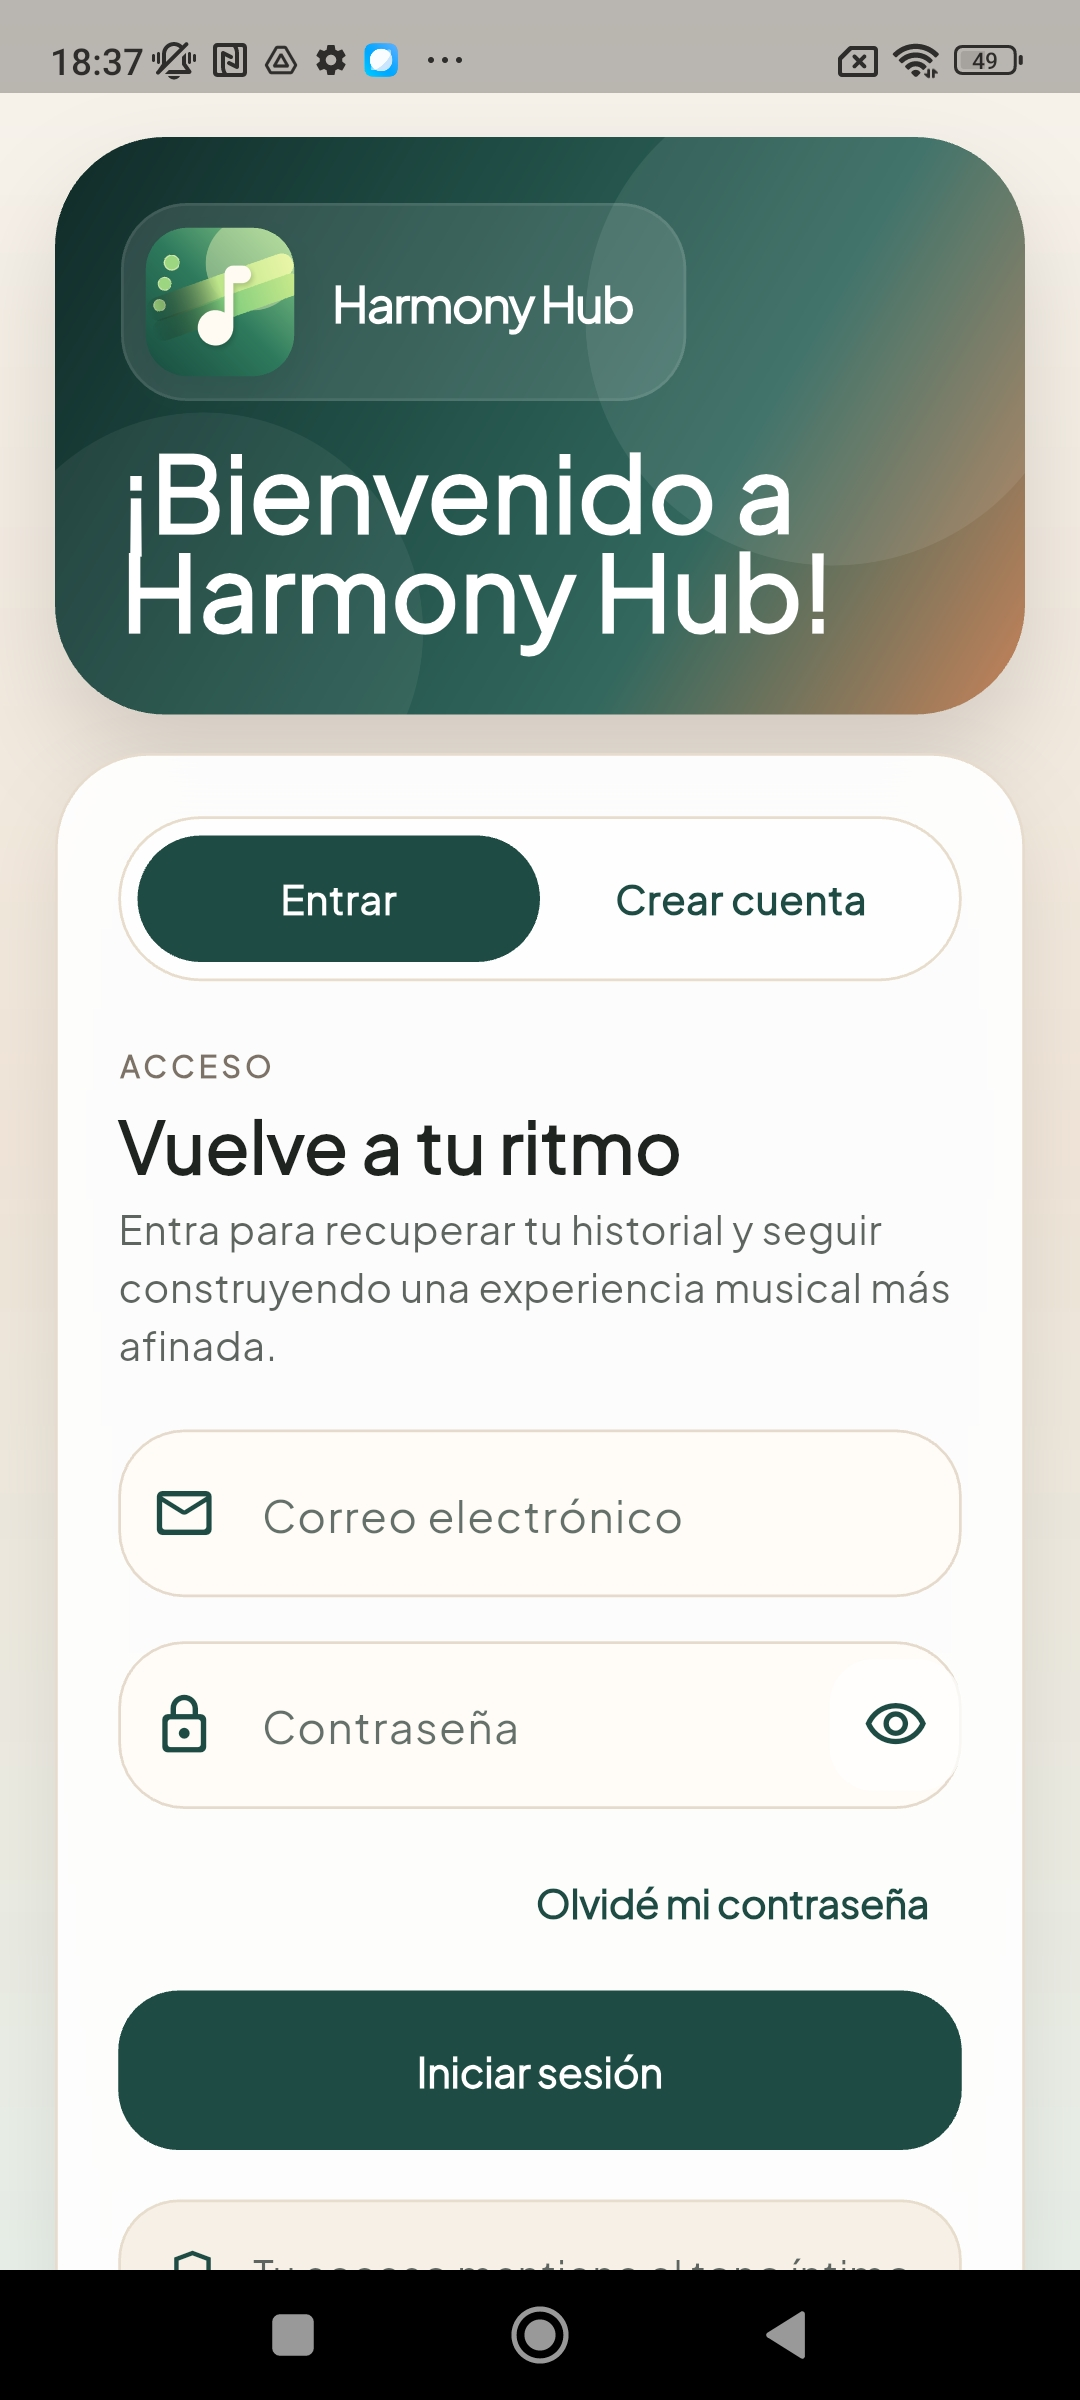
\includegraphics[width=\linewidth]{Imagenes/manual_app/Screenshot_2026-05-25-18-37-08-051_com.example.harmonyhub.jpg}
    \end{minipage}
    \hfill
    \begin{minipage}{0.31\textwidth}
        \centering
        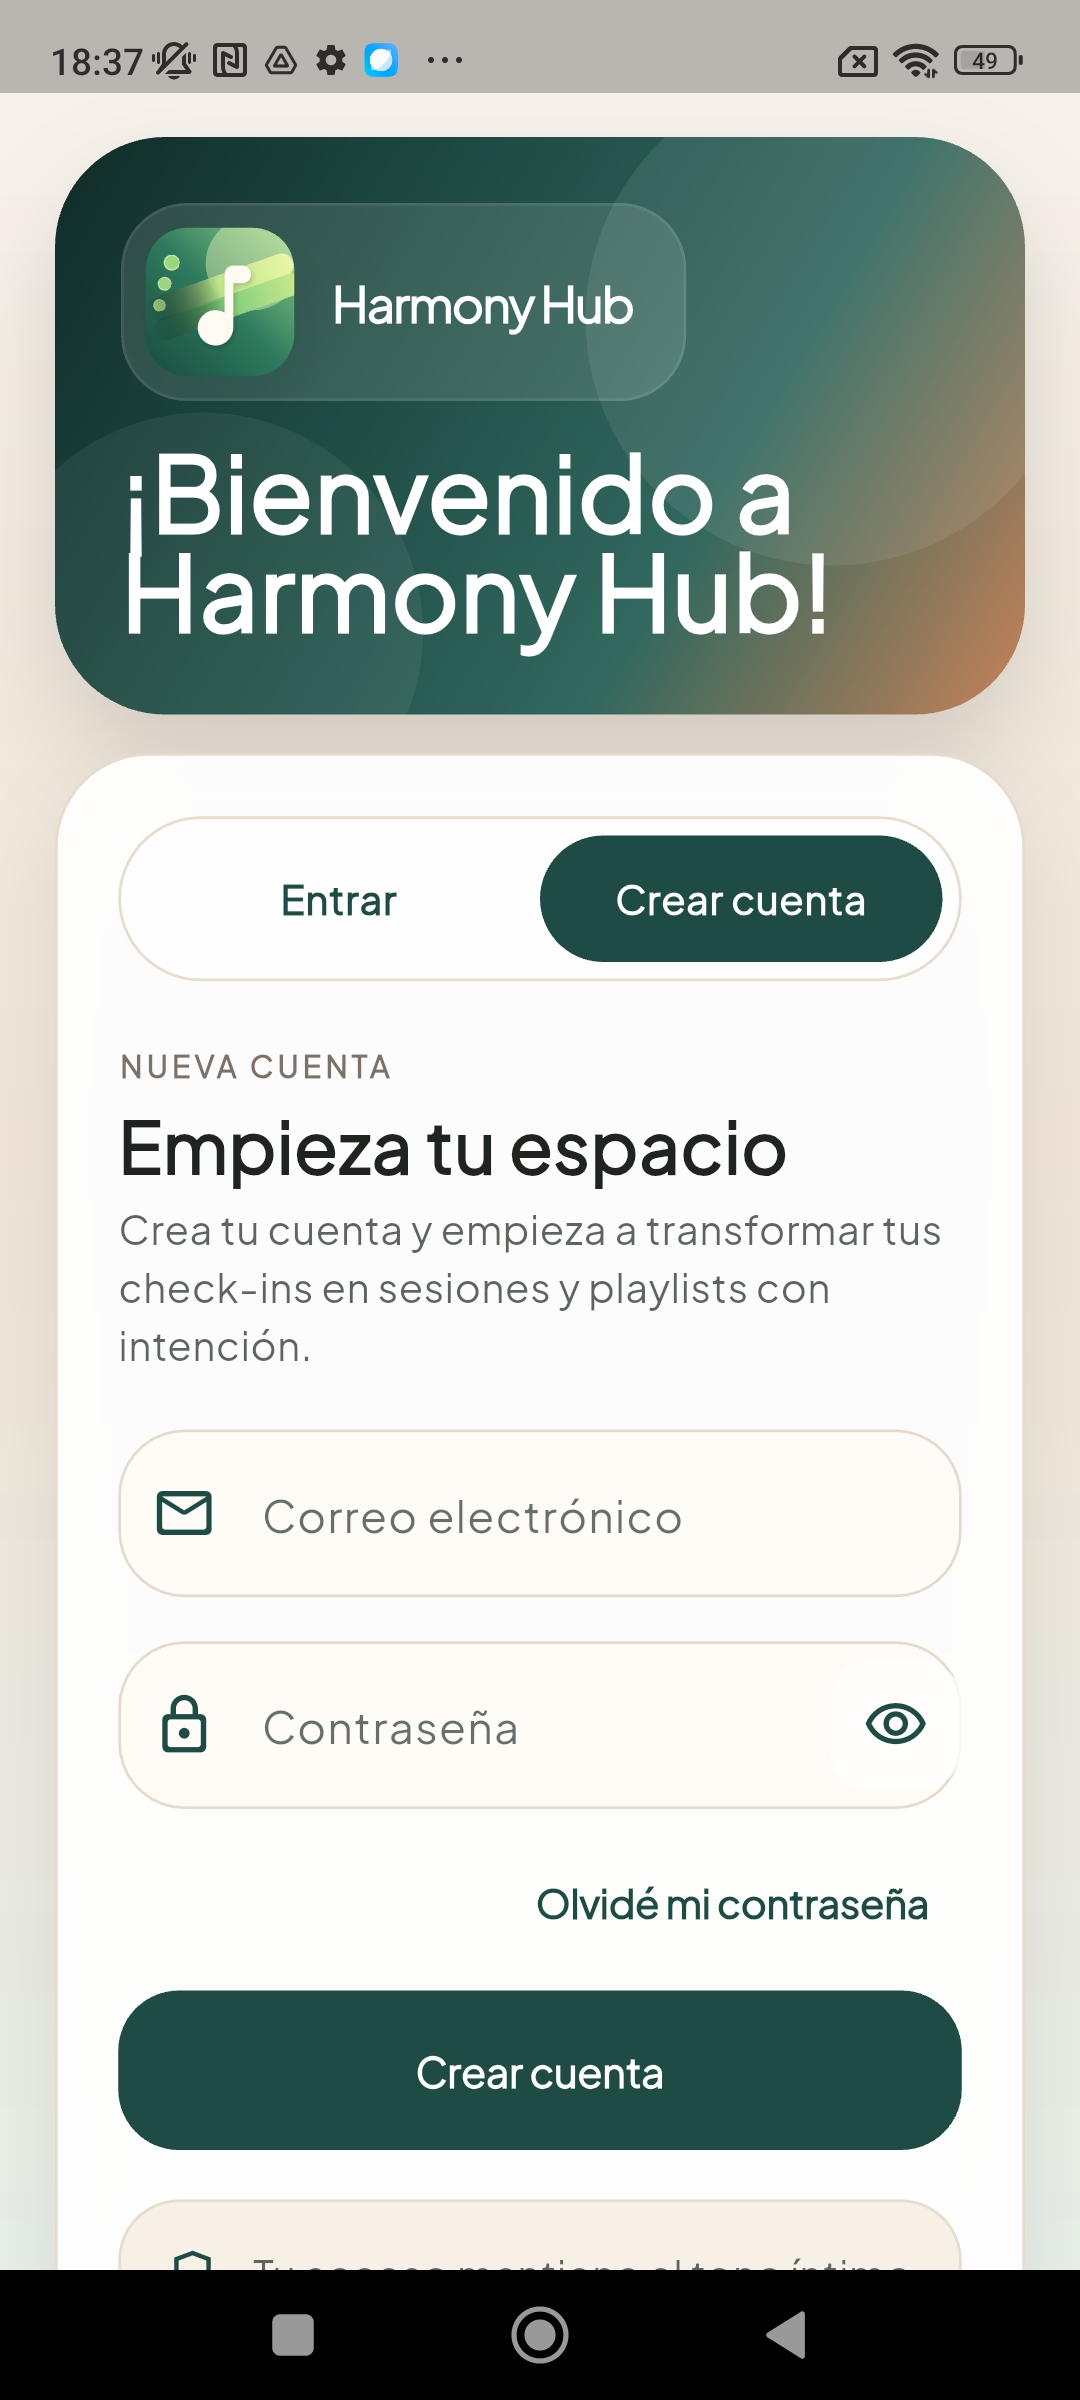
\includegraphics[width=\linewidth]{Imagenes/manual_app/Screenshot_2026-05-25-18-37-25-565_com.example.harmonyhub.jpg}
    \end{minipage}
    \hfill
    \begin{minipage}{0.31\textwidth}
        \centering
        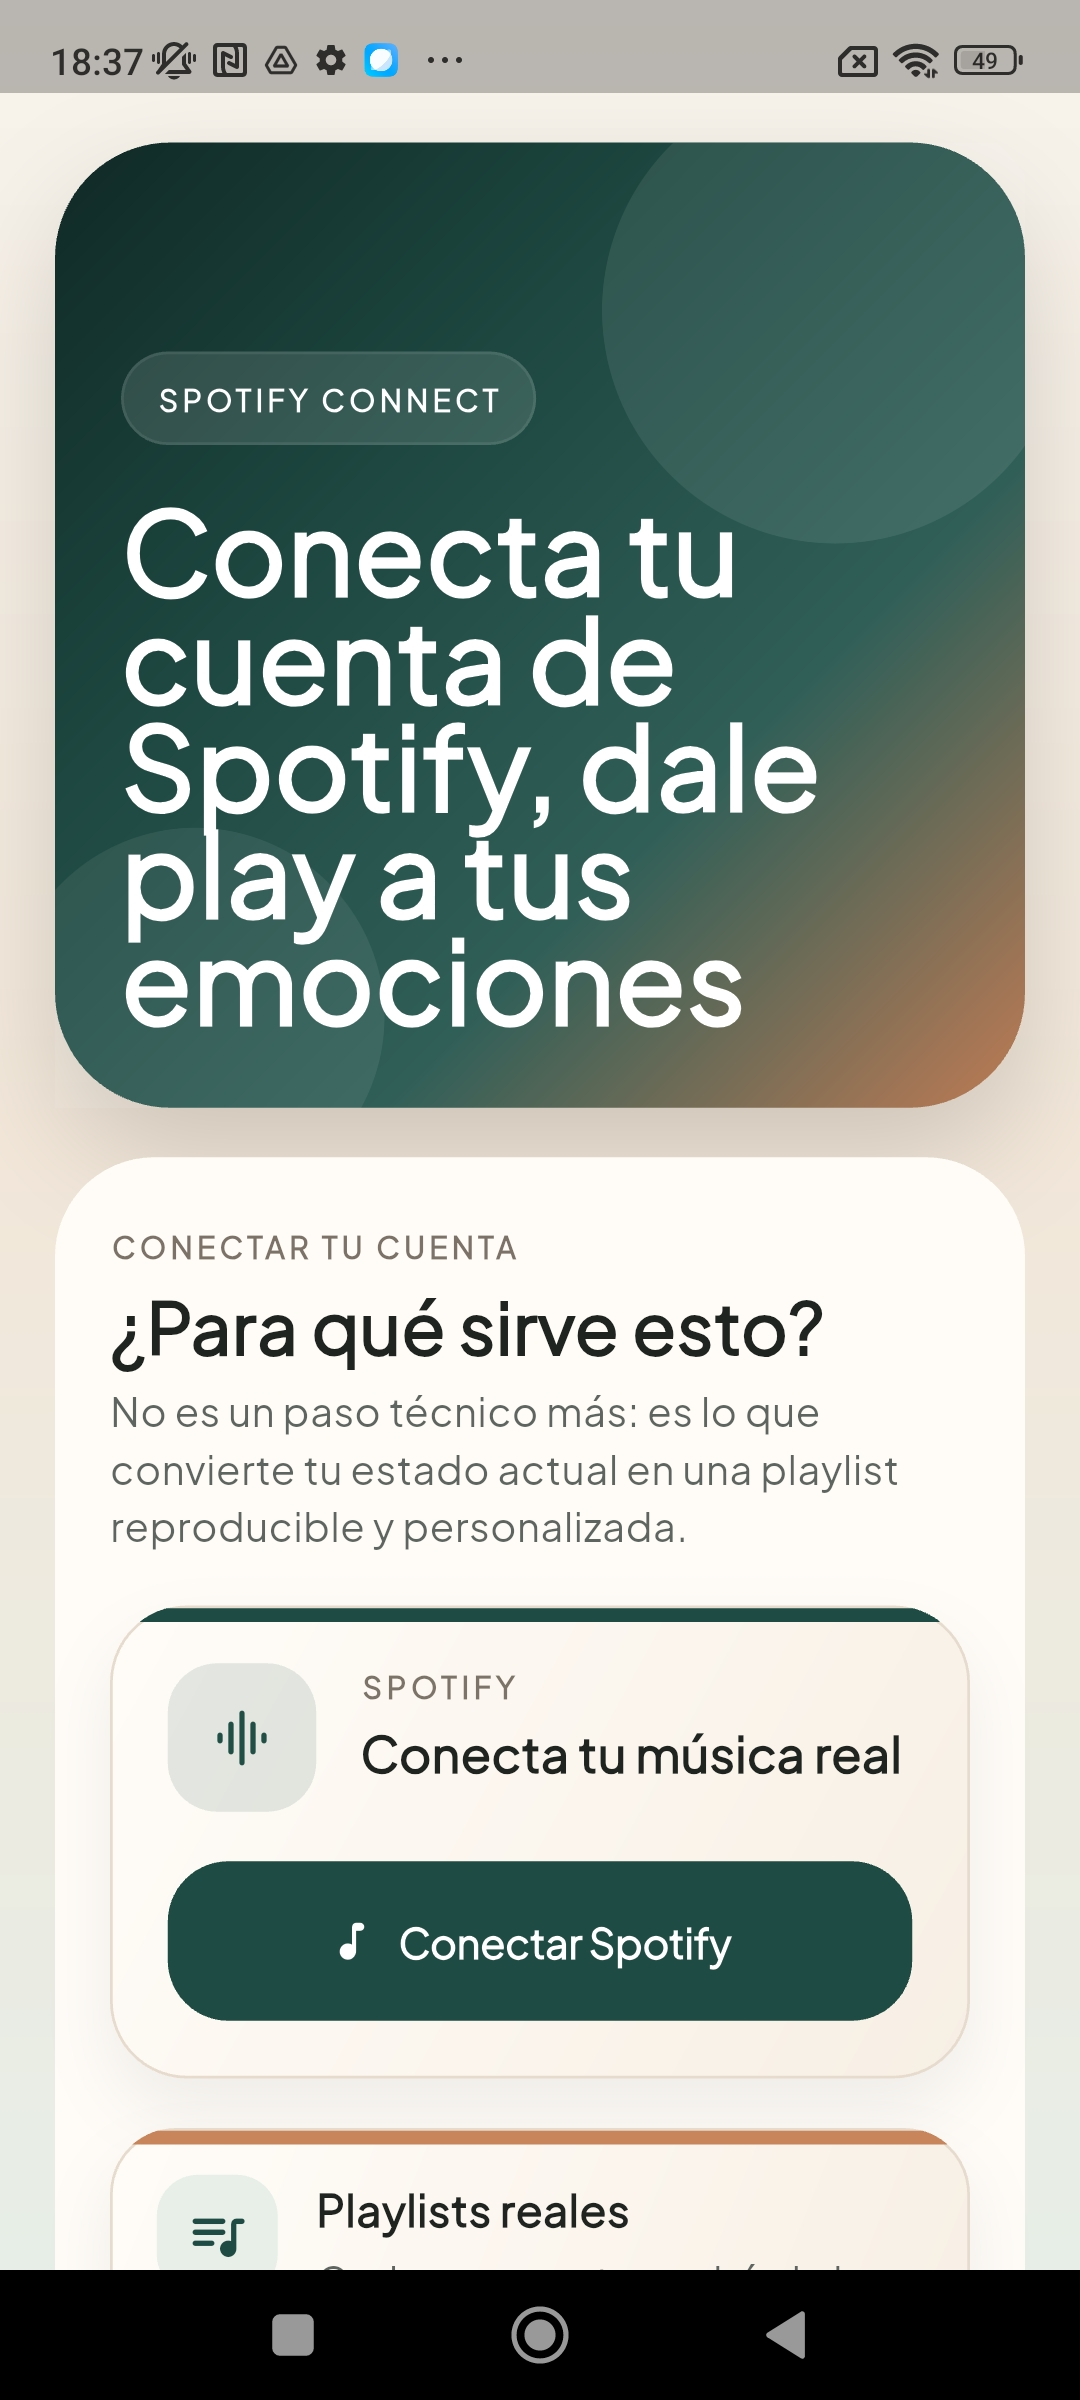
\includegraphics[width=\linewidth]{Imagenes/manual_app/Screenshot_2026-05-25-18-37-46-036_com.example.harmonyhub.jpg}
    \end{minipage}
    \caption{Pantallas iniciales del flujo de acceso: bienvenida e inicio de
    sesión, creación de cuenta y conexión obligatoria con Spotify antes de
    generar playlists reales.}
    \label{fig:manual_acceso_spotify}
\end{figure}

La figura~\ref{fig:manual_acceso_spotify} muestra el primer tramo del flujo de
uso. Primero aparece la pantalla de acceso, desde la que es posible iniciar
sesión o registrar una cuenta nueva. Una vez autenticada la persona usuaria, la
app solicita la conexión con Spotify, ya que esta integración es la que permite
materializar la recomendación final como playlist reproducible.

\section{Uso básico}
\label{sec:manual_usuario_uso_basico}

El flujo de uso normal puede resumirse en seis pasos:

\begin{enumerate}
    \item \textbf{Iniciar un check-in.} El usuario accede a la pantalla de
    check-in y responde preguntas breves sobre su momento actual.
    \item \textbf{Indicar el objetivo de la sesión.} Puede elegir, por ejemplo,
    foco, relajación o energía.
    \item \textbf{Ajustar preferencias.} La app permite indicar intensidad,
    preferencia vocal, nivel de exploración, popularidad deseada y resultado
    esperado.
    \item \textbf{Analizar el entorno si se desea.} Opcionalmente puede medir
    el contexto acústico del momento.
    \item \textbf{Generar la recomendación.} La aplicación muestra la sesión
    sugerida y, si el usuario la acepta, permite crear la playlist real.
    \item \textbf{Cerrar con feedback.} Tras escuchar la playlist, el usuario
    puede valorar si le resultó útil y cómo terminó la sesión.
\end{enumerate}

\subsection*{Pantalla principal y acceso al check-in}

\begin{figure}[htbp]
    \centering
    \begin{minipage}{0.47\textwidth}
        \centering
        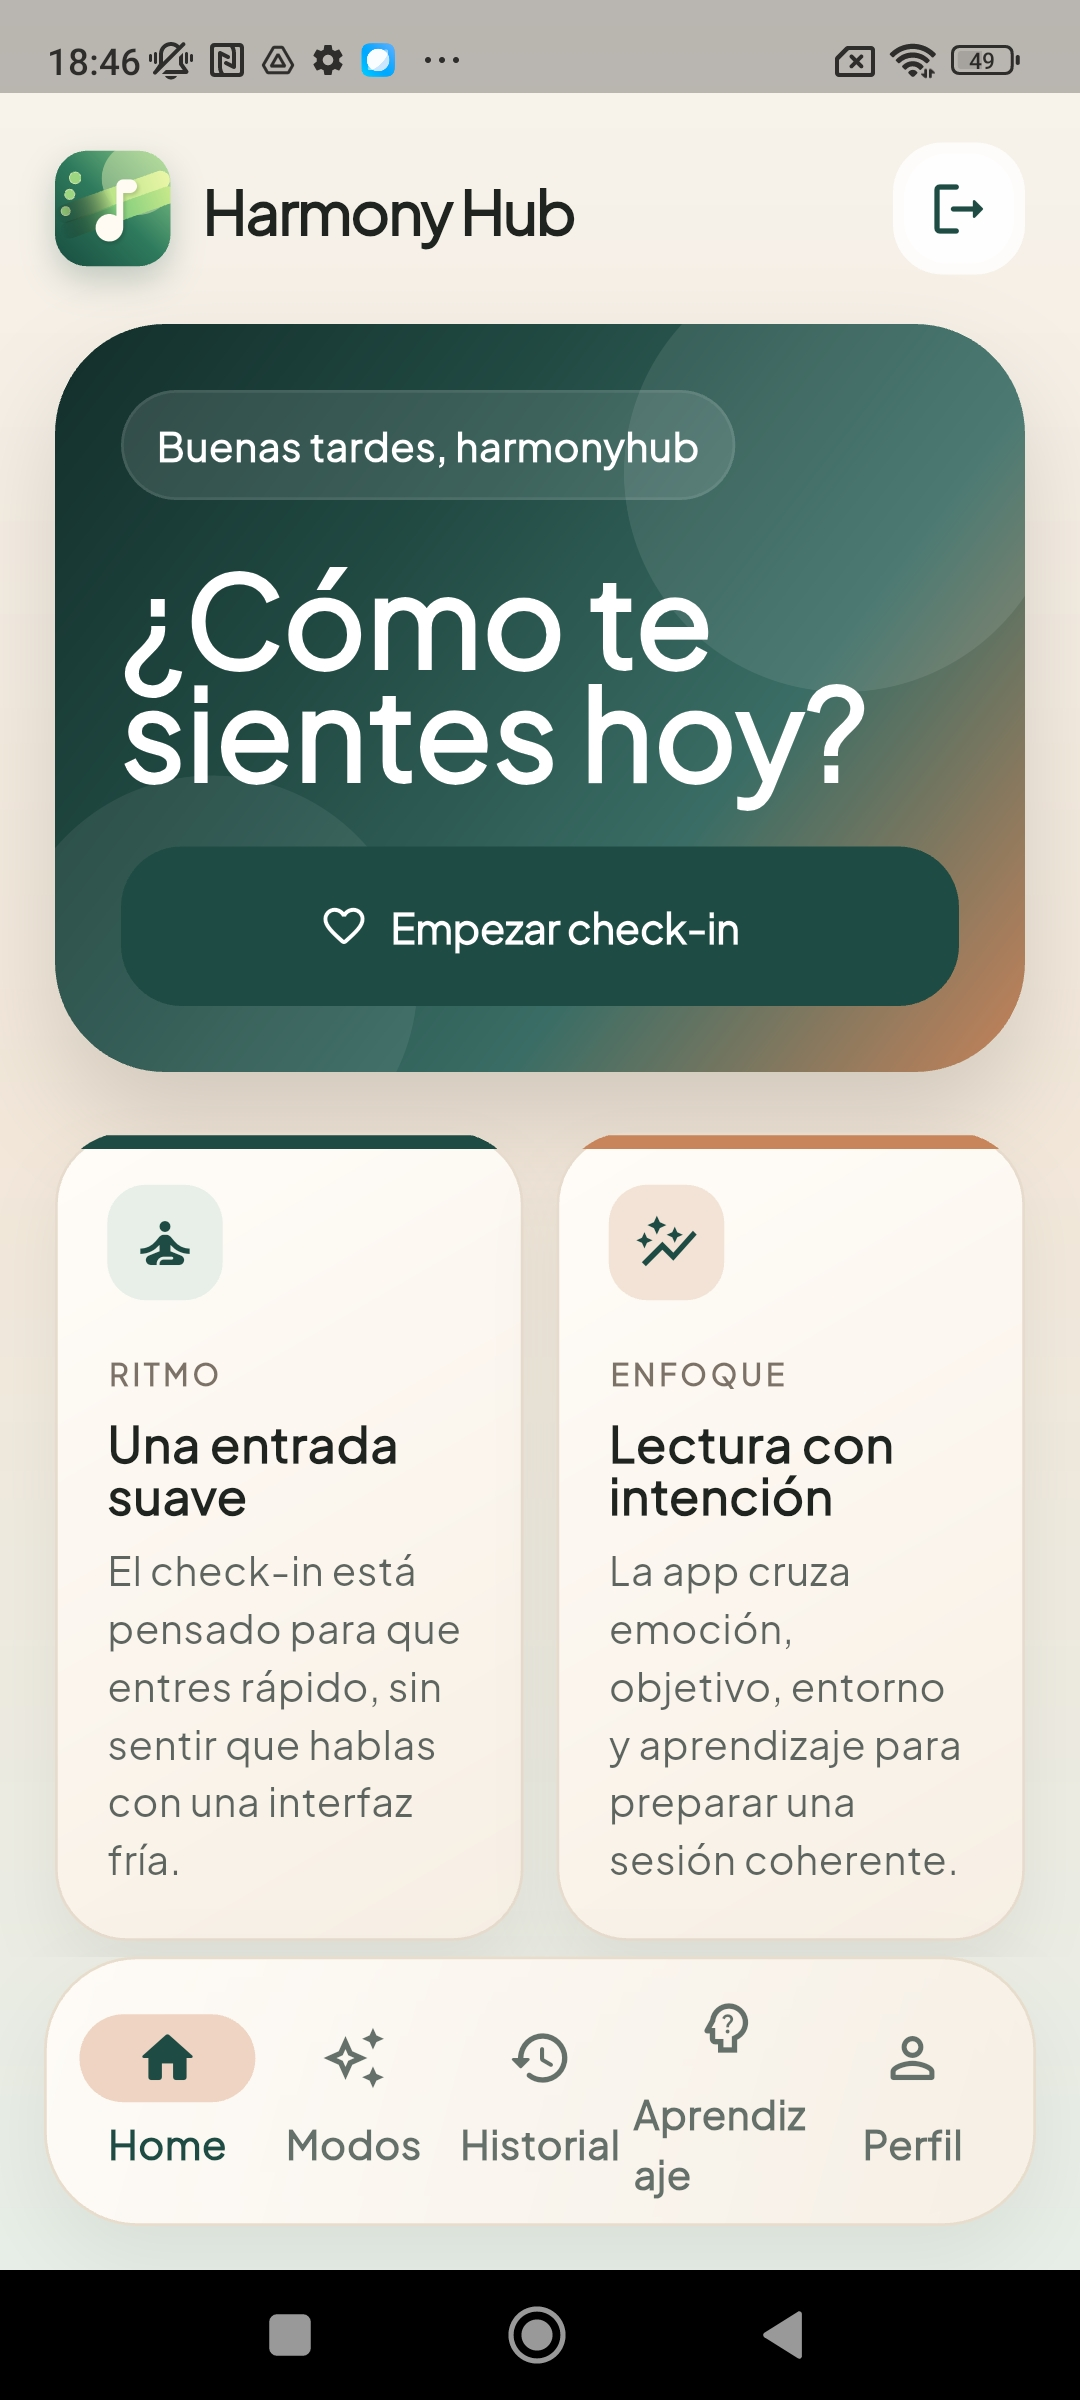
\includegraphics[width=\linewidth]{Imagenes/manual_app/Screenshot_2026-05-25-18-46-14-698_com.example.harmonyhub.jpg}
    \end{minipage}
    \hfill
    \begin{minipage}{0.47\textwidth}
        \centering
        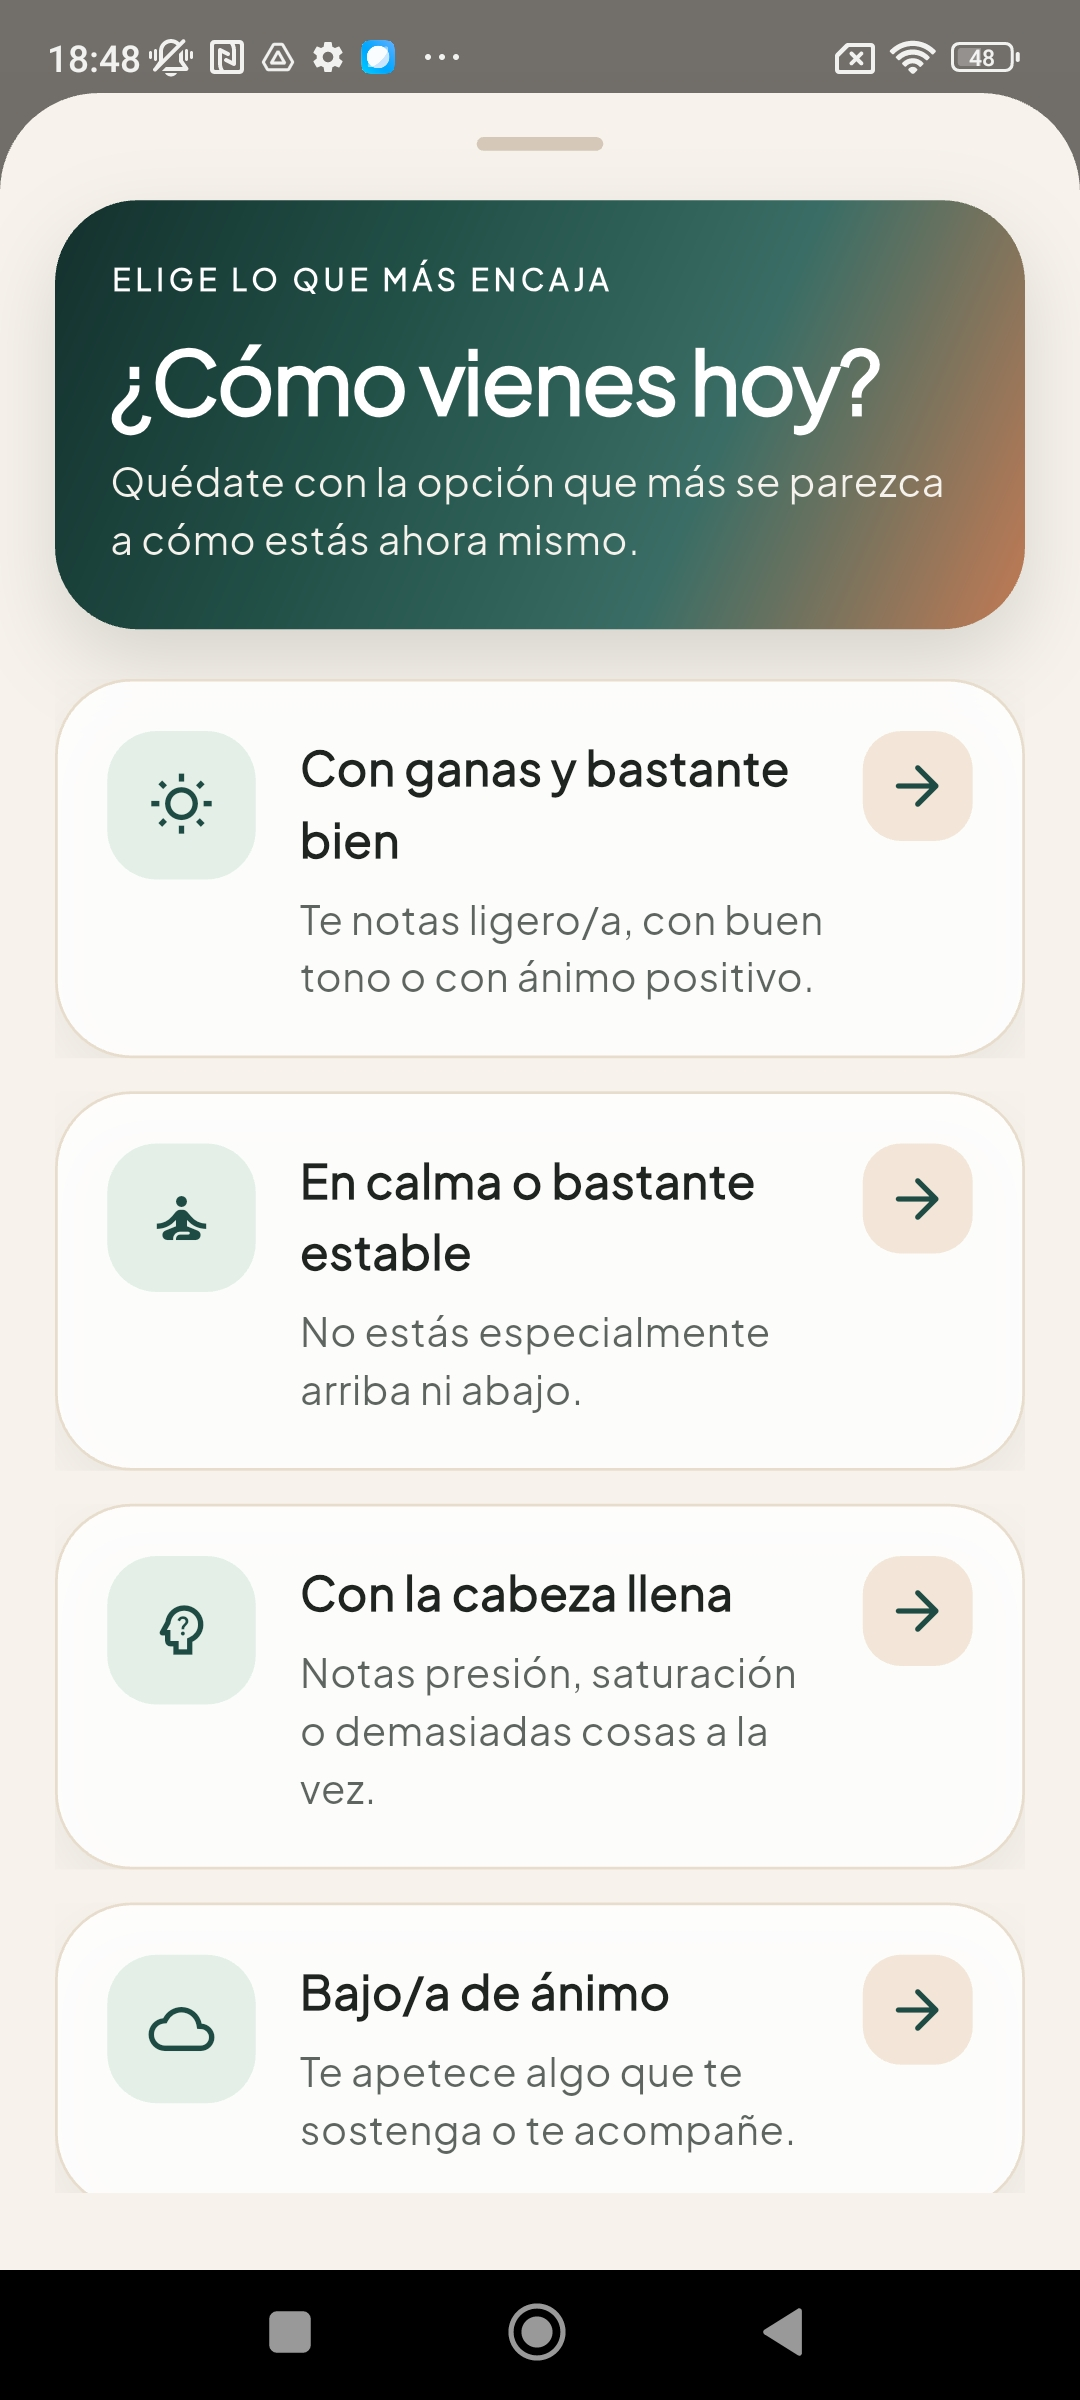
\includegraphics[width=\linewidth]{Imagenes/manual_app/Screenshot_2026-05-25-18-48-36-091_com.example.harmonyhub.jpg}
    \end{minipage}
    \caption{Pantalla principal y comienzo del check-in. A la izquierda se ve
    la portada con acceso directo a \textit{Empezar check-in}; a la derecha,
    una de las preguntas guiadas del flujo conversacional.}
    \label{fig:manual_home_checkin}
\end{figure}

La portada actúa como punto de entrada del producto. Desde ella se puede
empezar el check-in, consultar accesos a otros bloques y moverse por la
navegación inferior. Durante el check-in, Harmony Hub presenta preguntas breves
en lenguaje natural para recoger estado emocional, objetivo, energía, estrés y
preferencias sin exigir una interacción técnica.

\subsection*{Entorno acústico y generación de la recomendación}

\begin{figure}[htbp]
    \centering
    \begin{minipage}{0.47\textwidth}
        \centering
        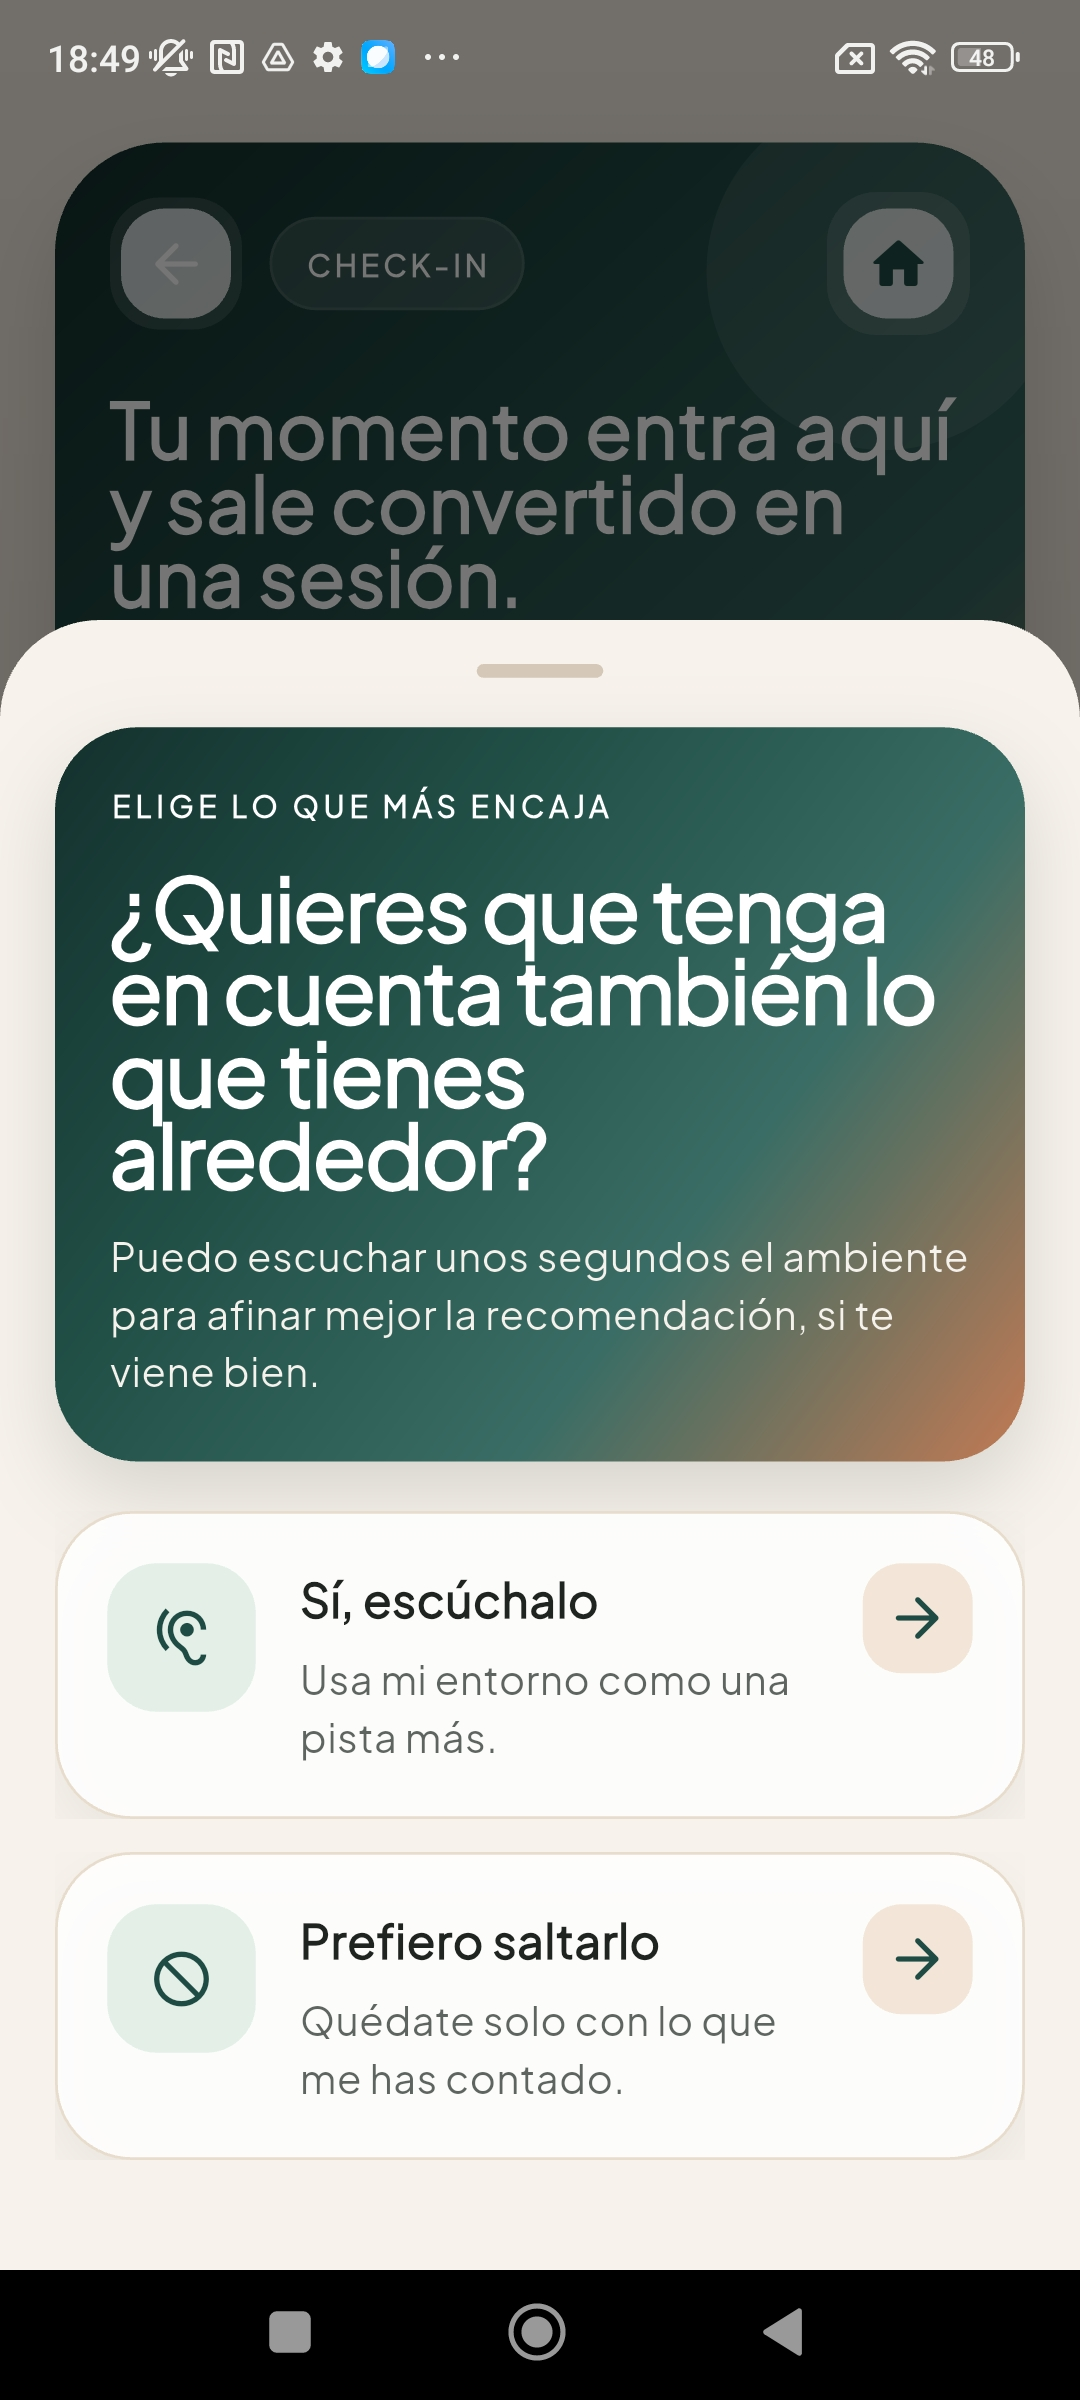
\includegraphics[width=\linewidth]{Imagenes/manual_app/Screenshot_2026-05-25-18-49-26-089_com.example.harmonyhub.jpg}
    \end{minipage}
    \hfill
    \begin{minipage}{0.47\textwidth}
        \centering
        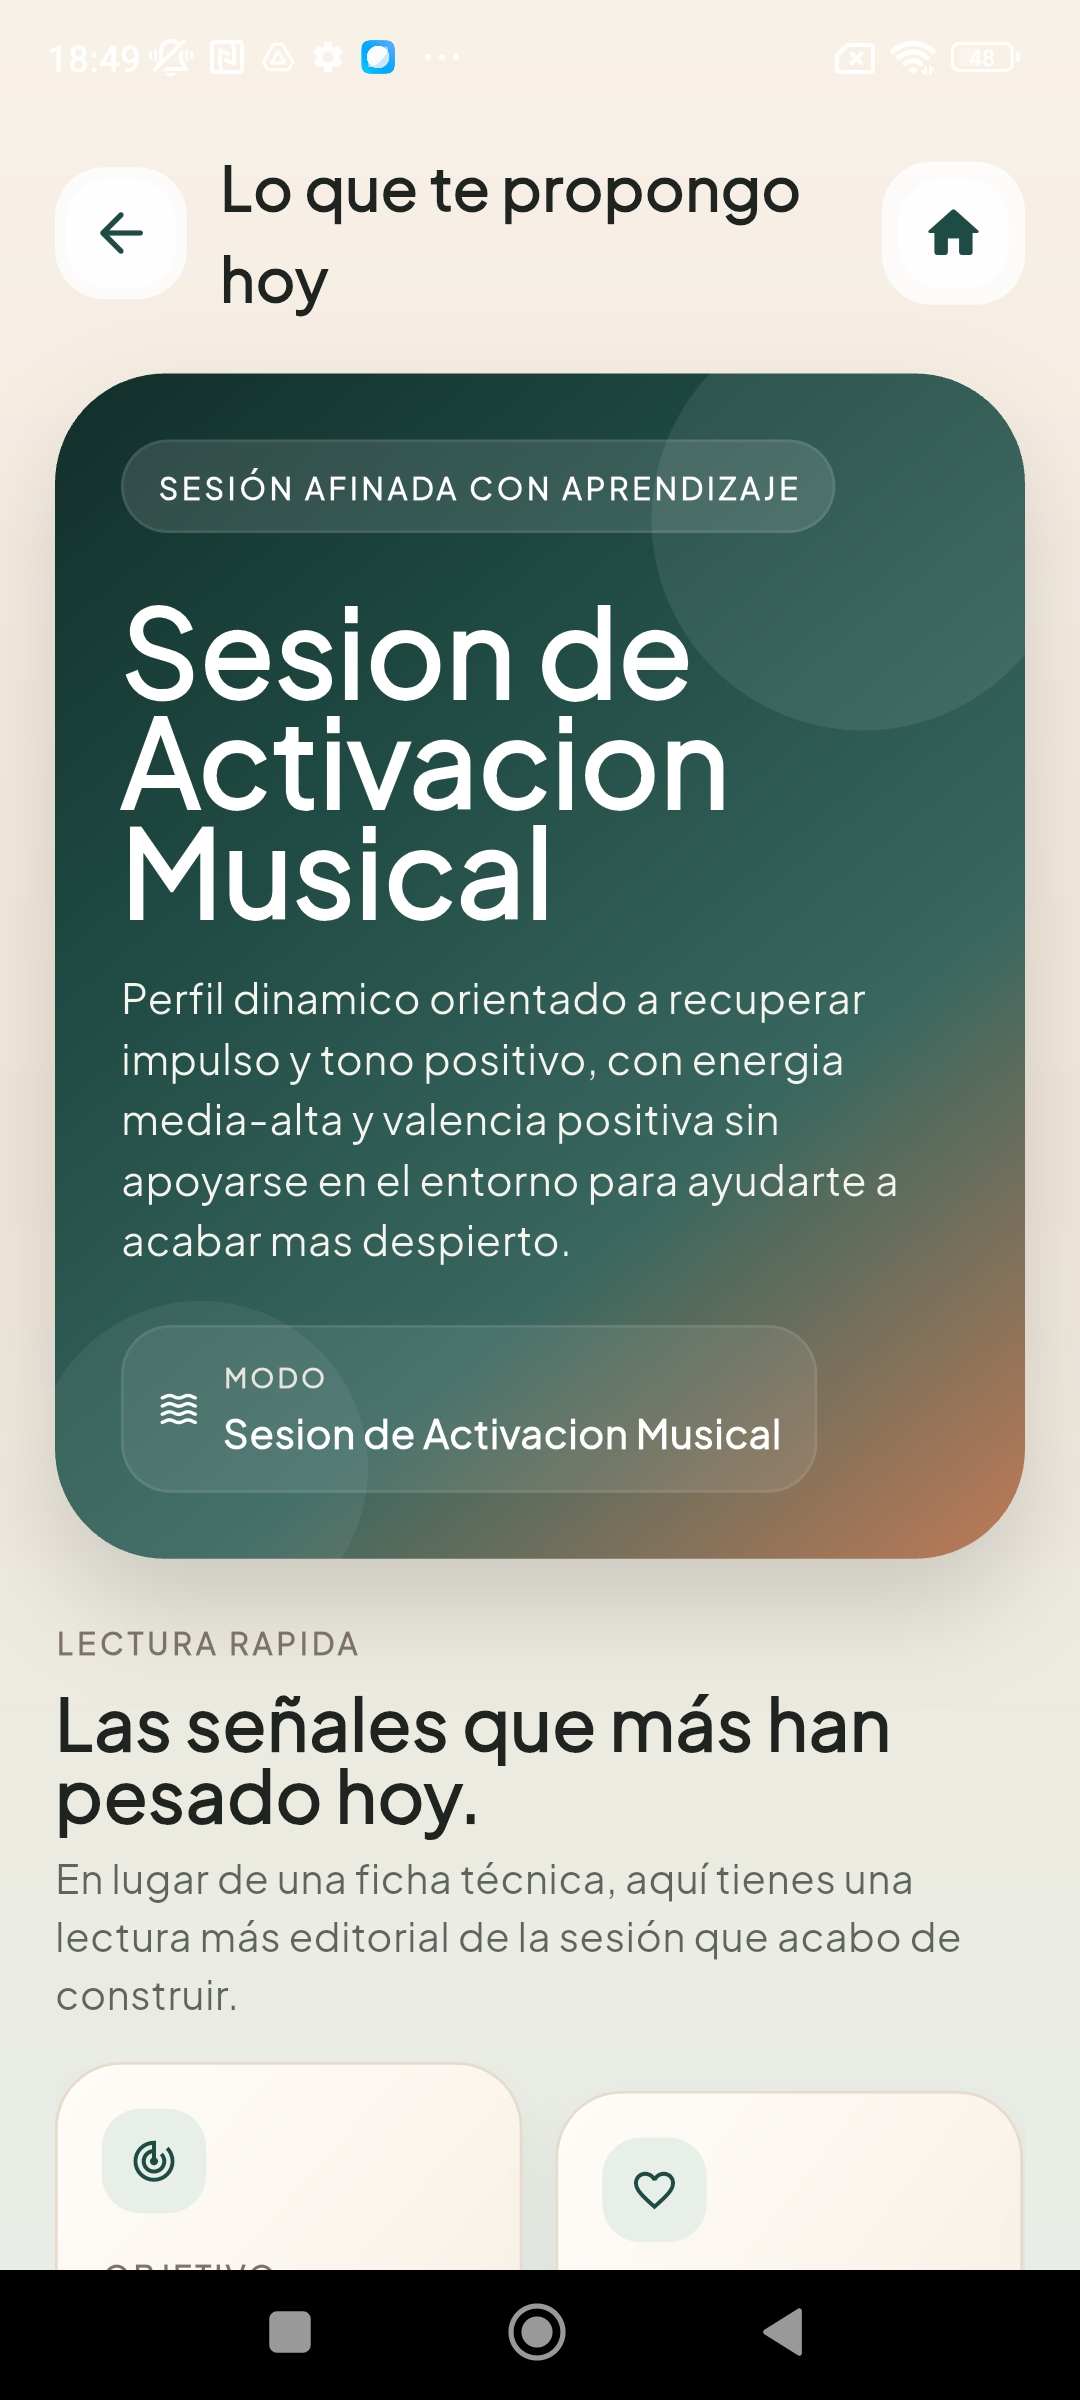
\includegraphics[width=\linewidth]{Imagenes/manual_app/Screenshot_2026-05-25-18-49-39-980_com.example.harmonyhub.jpg}
    \end{minipage}
    \caption{Activación opcional del análisis del entorno y presentación de la
    recomendación resultante.}
    \label{fig:manual_entorno_recomendacion}
\end{figure}

El análisis del entorno es opcional. Si la persona usuaria acepta, la app
escucha unos segundos el ambiente para utilizar esa señal como contexto
adicional. Después, se presenta una recomendación editorializada con el tipo de
sesión sugerido, una explicación funcional y un resumen del modo elegido.

\subsection*{Uso del aprendizaje acumulado y creación de la playlist}

\begin{figure}[htbp]
    \centering
    \begin{minipage}{0.47\textwidth}
        \centering
        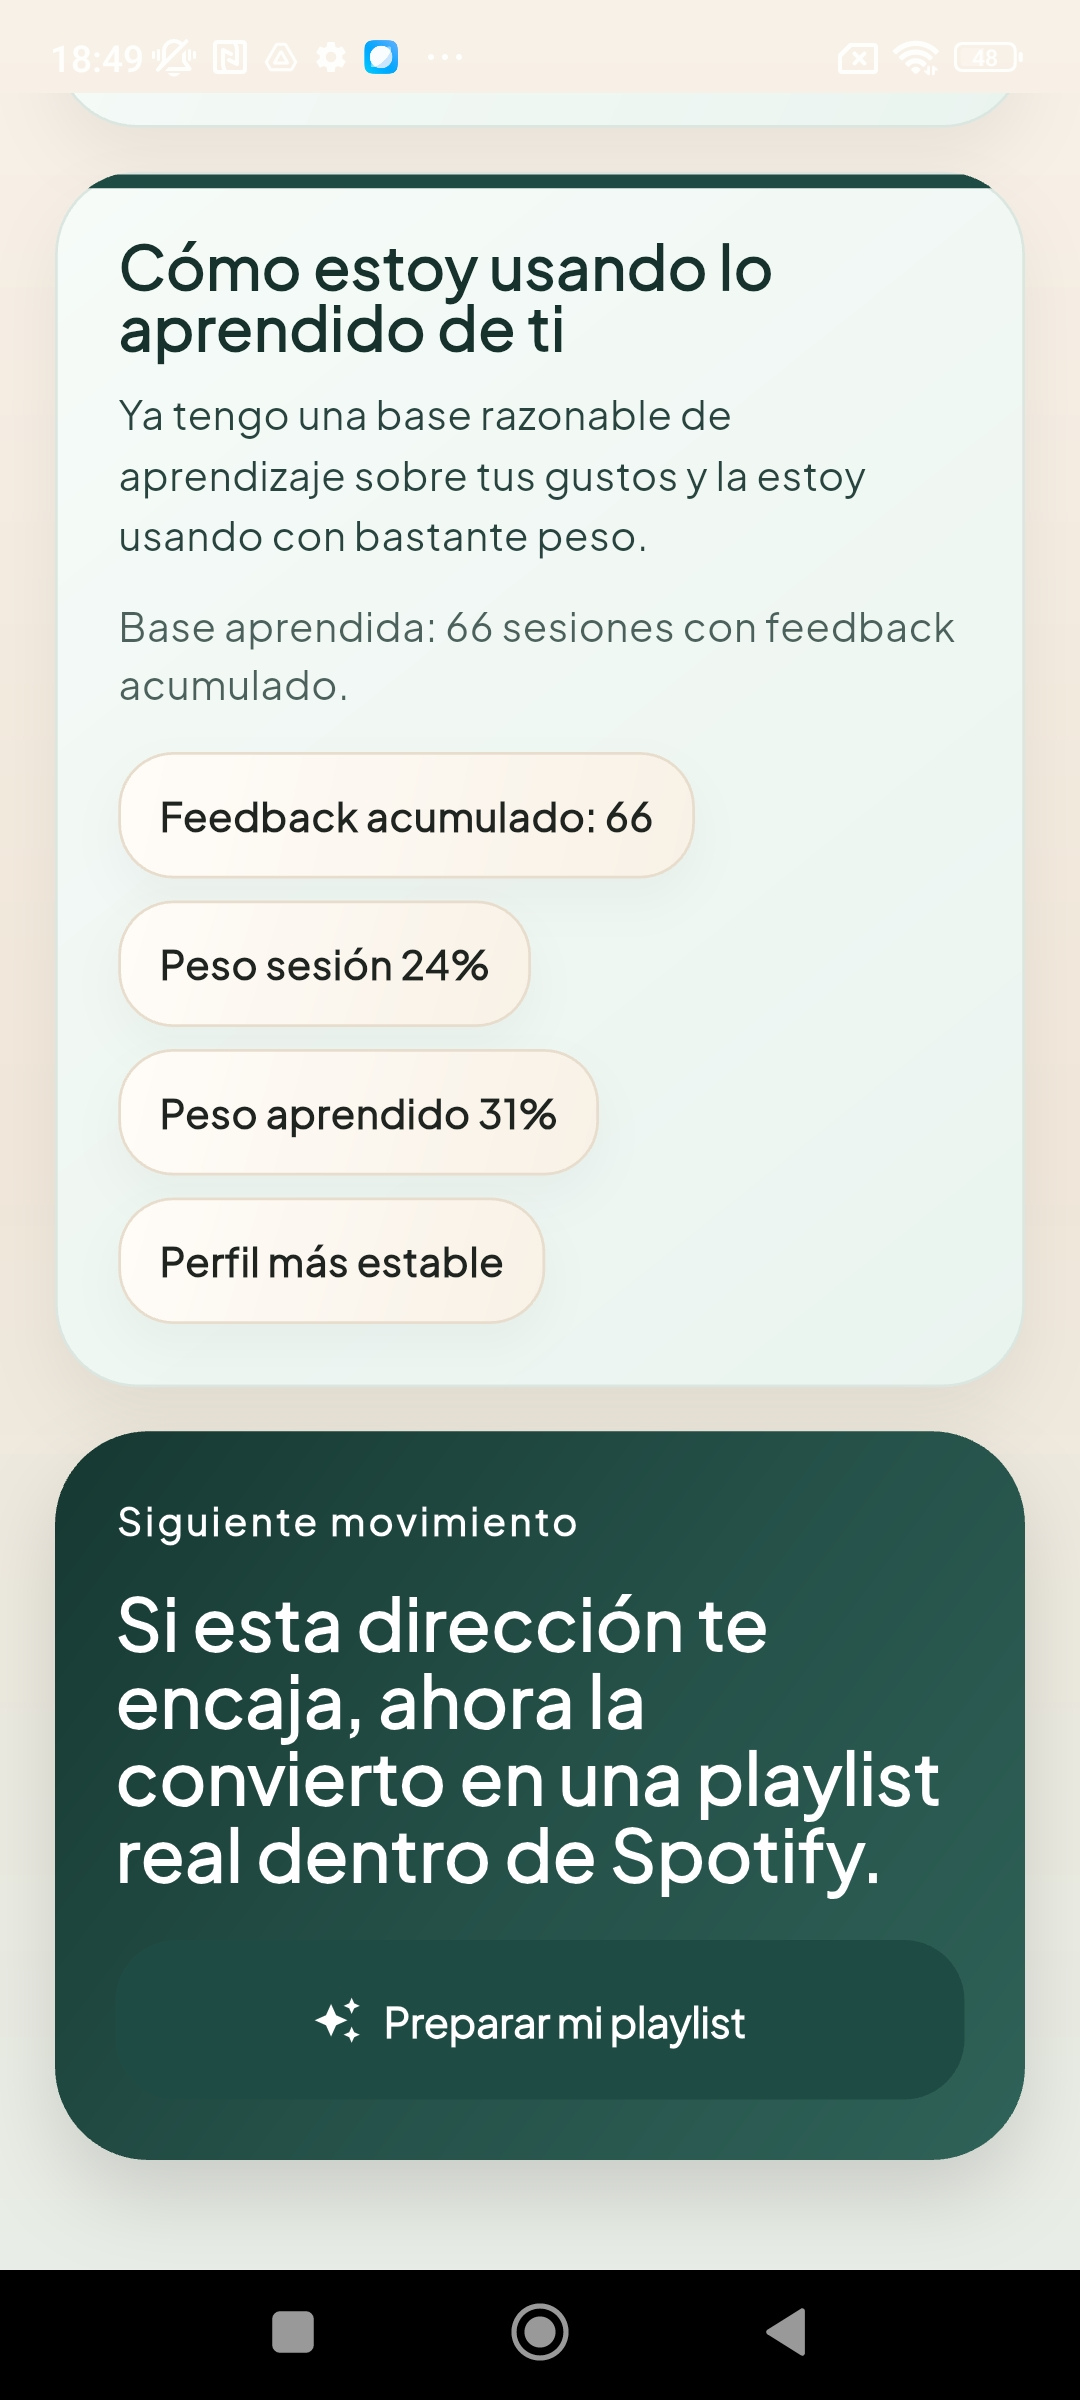
\includegraphics[width=\linewidth]{Imagenes/manual_app/Screenshot_2026-05-25-18-49-46-860_com.example.harmonyhub.jpg}
    \end{minipage}
    \hfill
    \begin{minipage}{0.47\textwidth}
        \centering
        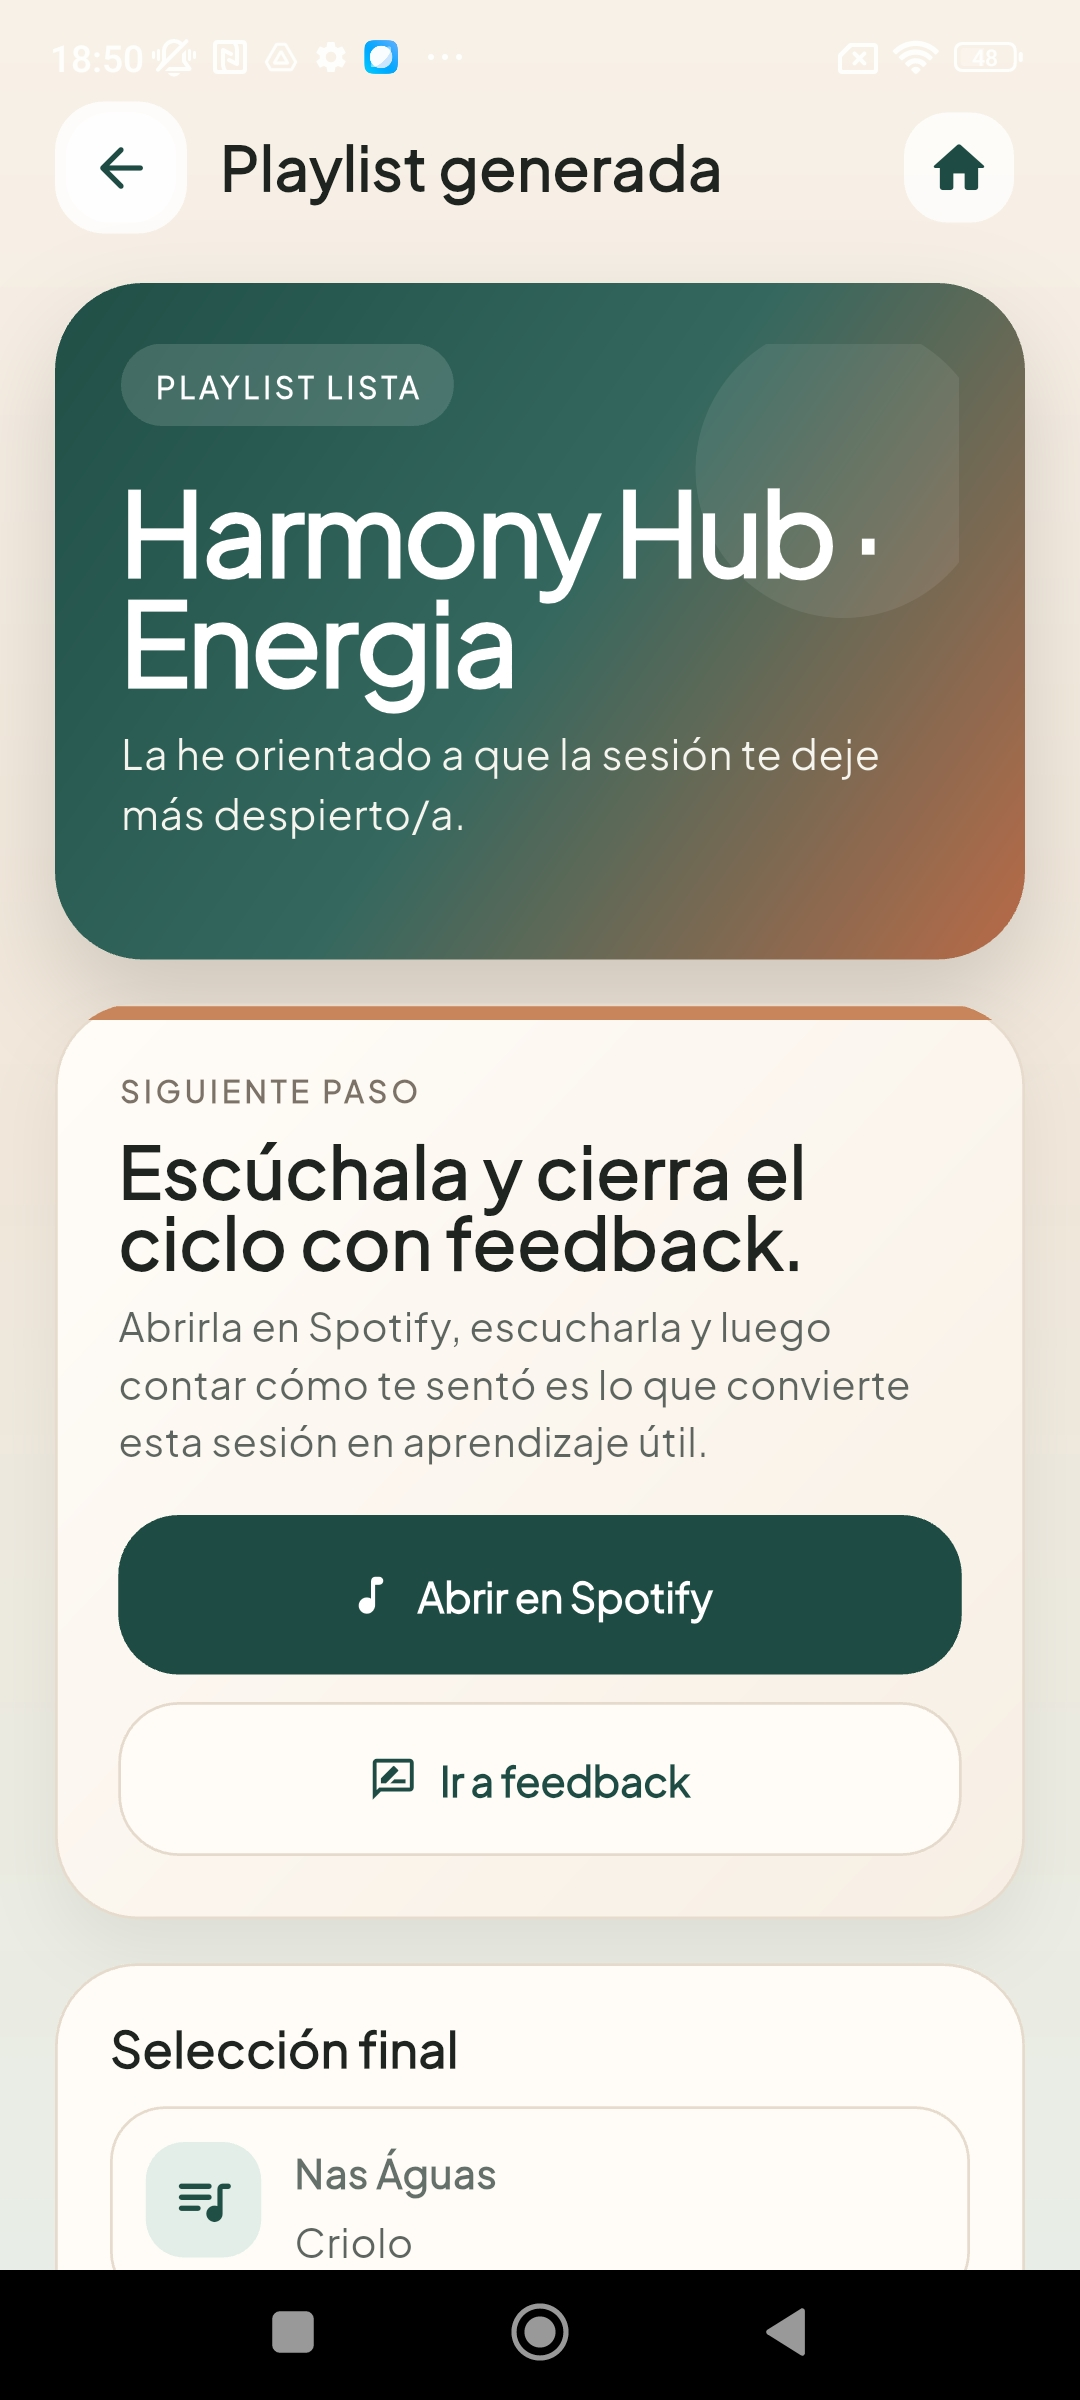
\includegraphics[width=\linewidth]{Imagenes/manual_app/Screenshot_2026-05-25-18-50-27-942_com.example.harmonyhub.jpg}
    \end{minipage}
    \caption{Explicación del peso del aprendizaje acumulado y pantalla de
    playlist ya generada dentro de la app.}
    \label{fig:manual_aprendizaje_playlist}
\end{figure}

Antes de crear la playlist, la recomendación puede mostrar cómo se está usando
el aprendizaje acumulado, incluyendo señales como el feedback disponible o el
peso relativo del perfil aprendido. Una vez generada la playlist, Harmony Hub
presenta el resultado final, permite abrirlo en Spotify y ofrece el acceso
directo al cierre con feedback.

\subsection*{Cierre de sesión y reproducción real en Spotify}

\begin{figure}[htbp]
    \centering
    \begin{minipage}{0.47\textwidth}
        \centering
        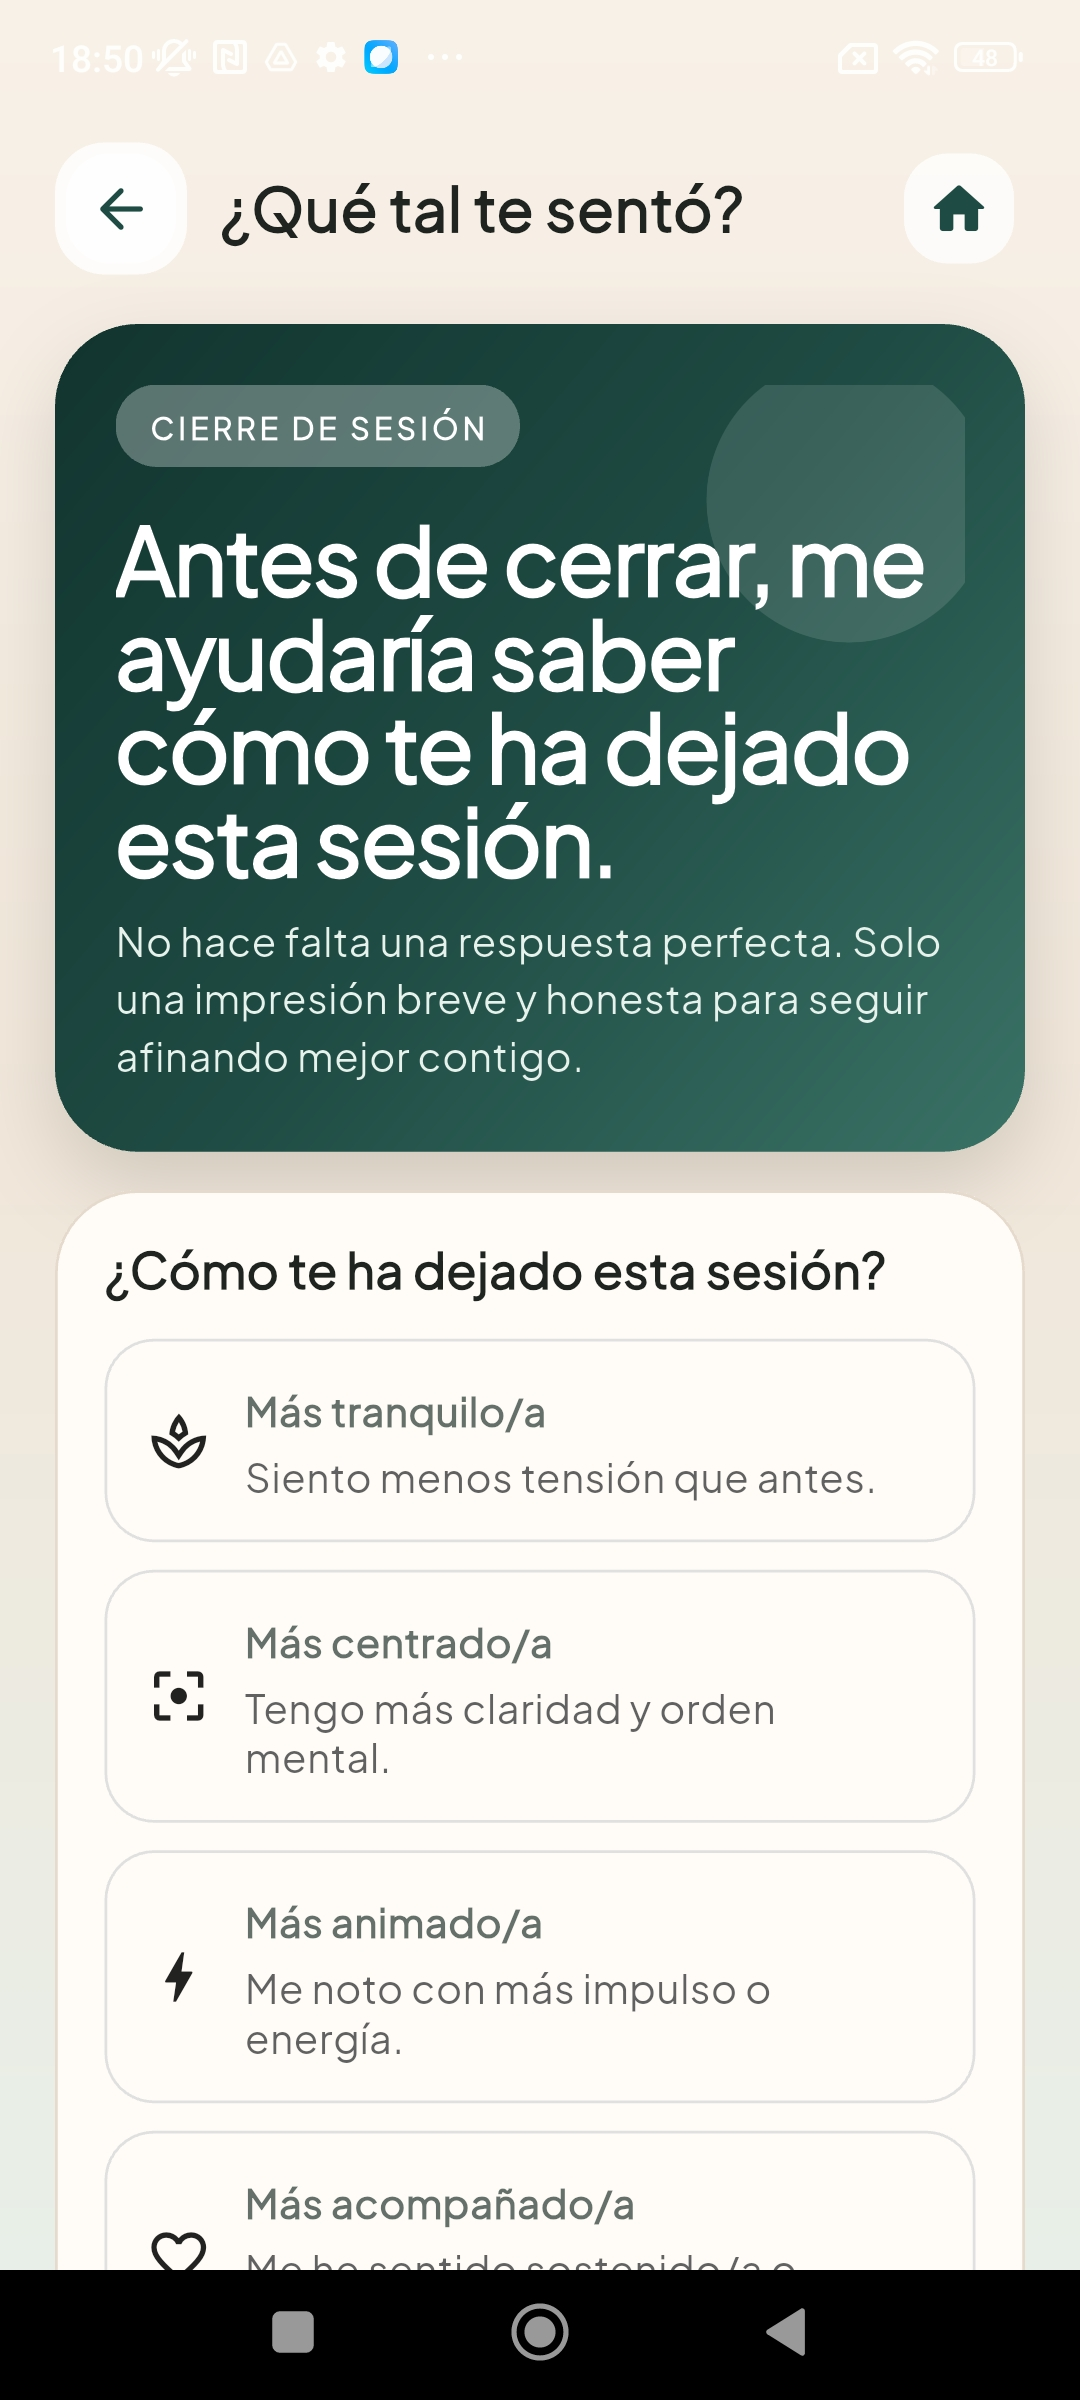
\includegraphics[width=\linewidth]{Imagenes/manual_app/Screenshot_2026-05-25-18-50-33-482_com.example.harmonyhub.jpg}
    \end{minipage}
    \hfill
    \begin{minipage}{0.47\textwidth}
        \centering
        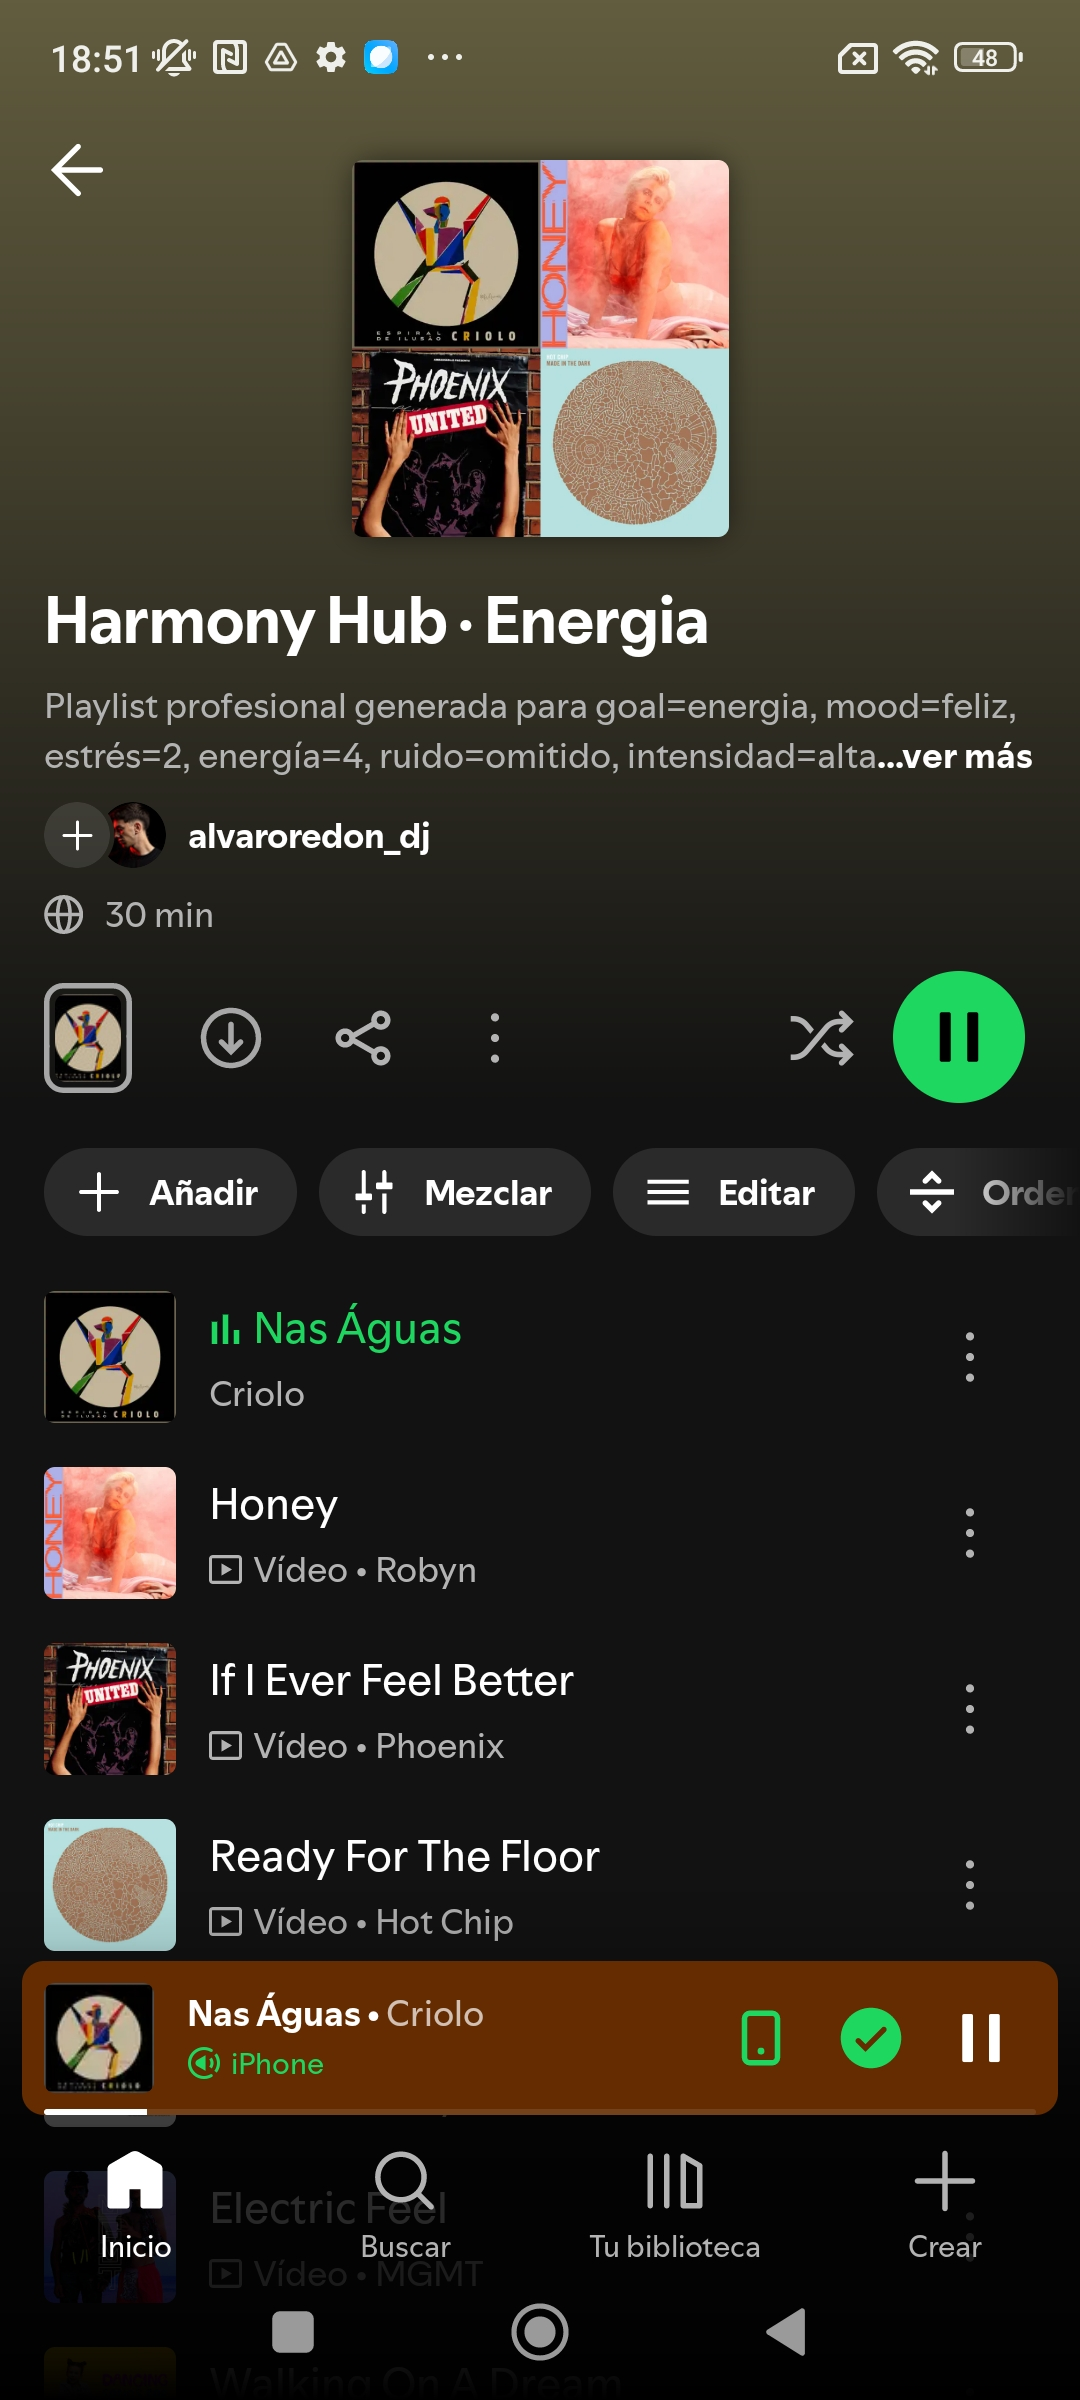
\includegraphics[width=\linewidth]{Imagenes/manual_app/Screenshot_2026-05-25-18-51-18-766_com.spotify.music.jpg}
    \end{minipage}
    \caption{Pantalla de feedback al cerrar la sesión y ejemplo de playlist
    abierta y reproducida ya dentro de Spotify.}
    \label{fig:manual_feedback_spotify}
\end{figure}

El ciclo de uso se cierra cuando la persona usuaria escucha la playlist y
responde cómo le ha dejado la sesión. Esta interacción es clave para el
aprendizaje posterior. La segunda imagen confirma además que la salida no se
queda en una sugerencia abstracta, sino que acaba convertida en una playlist
real dentro del ecosistema de Spotify.

\subsection*{Errores frecuentes y cómo interpretarlos}

Además del flujo correcto, resulta útil que la persona usuaria reconozca
algunos fallos previsibles y sepa qué significan. Las capturas siguientes no
representan errores arbitrarios, sino situaciones reales que pueden aparecer
durante el uso de la app y que conviene interpretar correctamente.

\begin{figure}[htbp]
    \centering
    \begin{minipage}{0.47\textwidth}
        \centering
        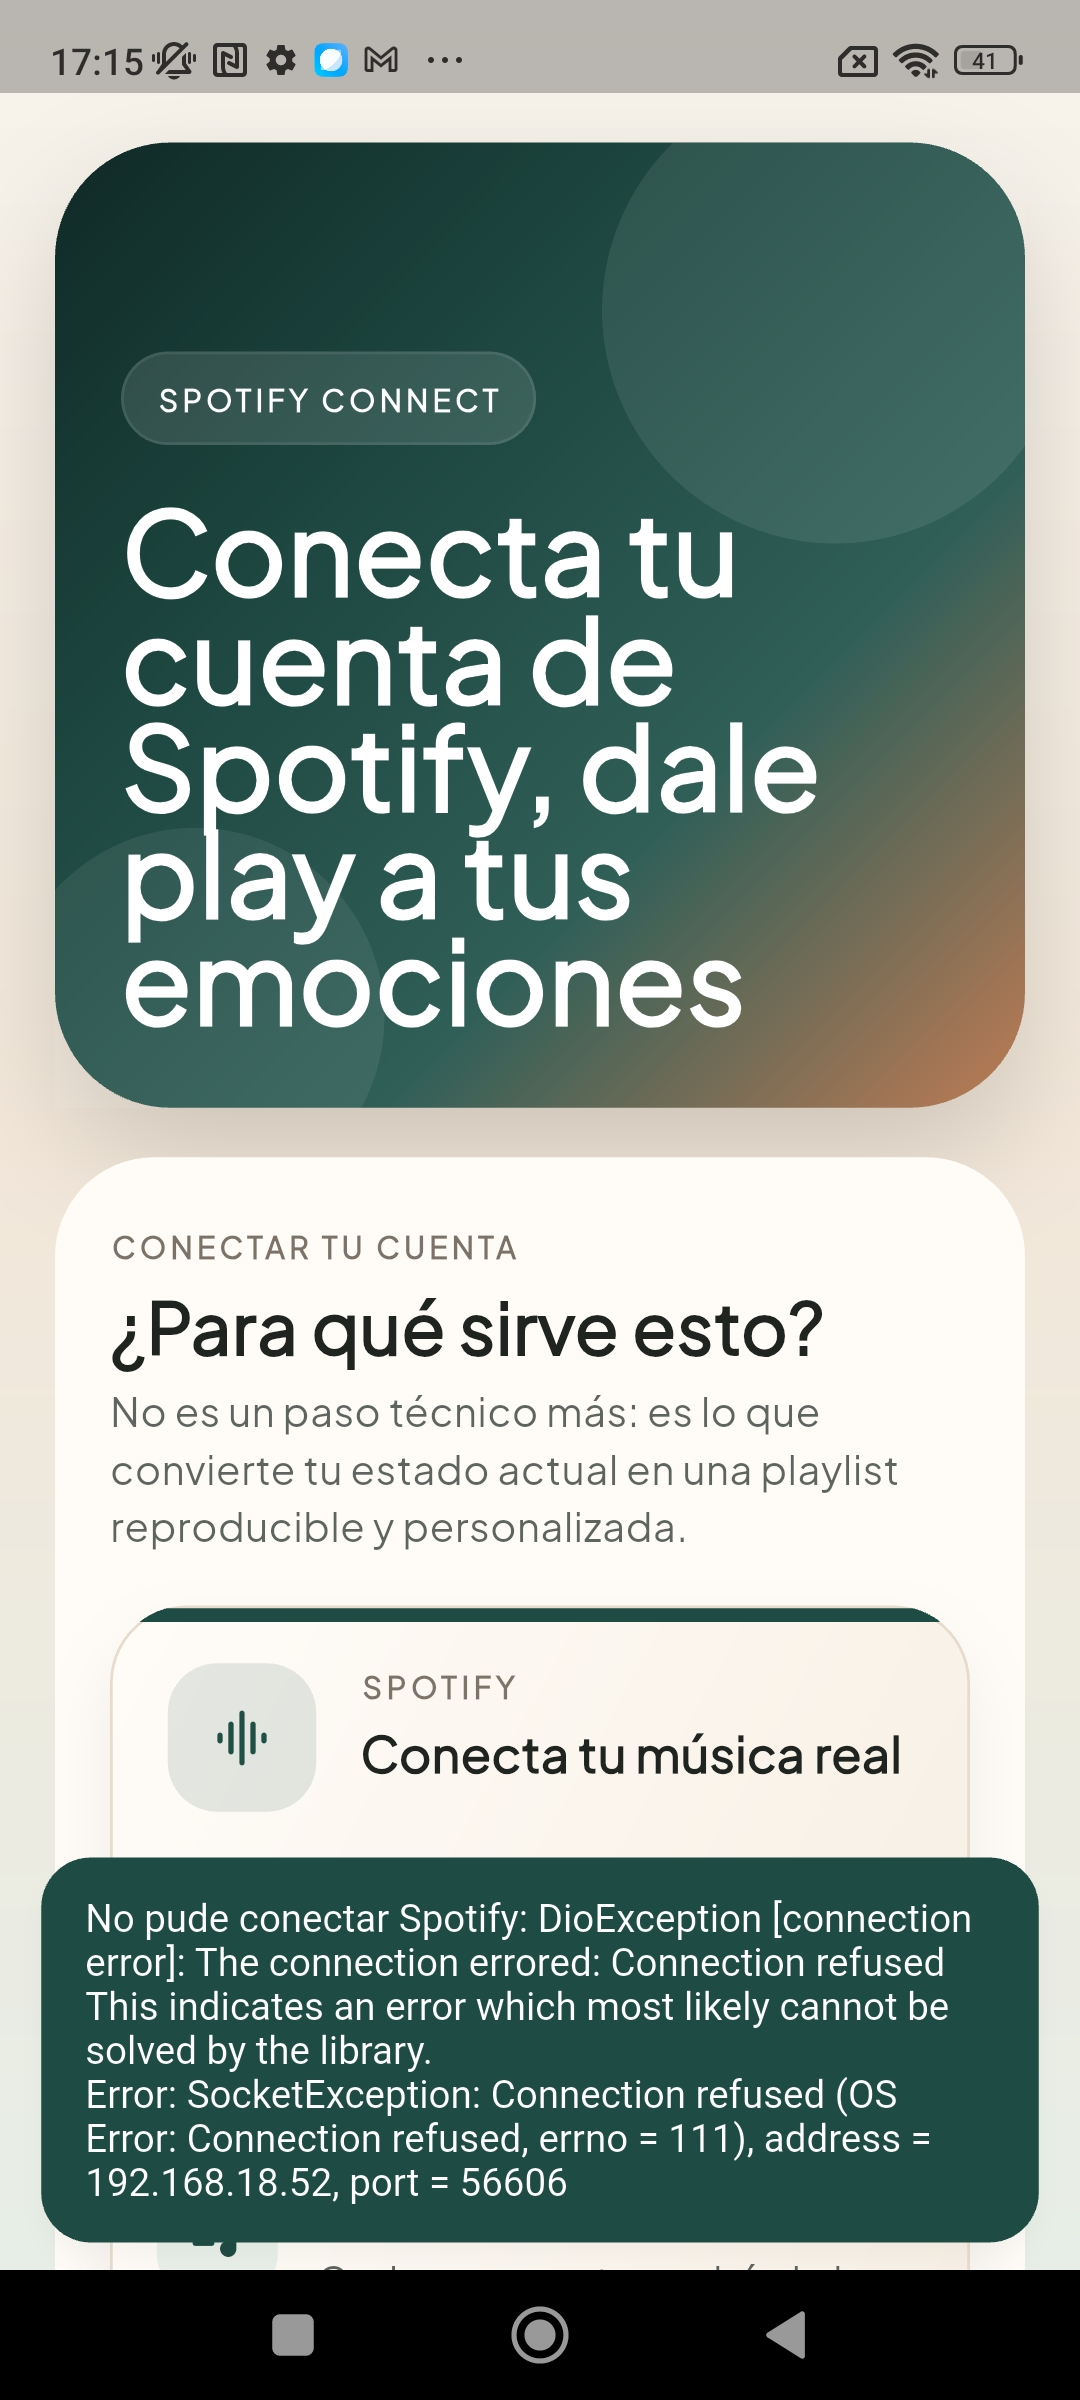
\includegraphics[width=\linewidth]{Imagenes/manual_errores/Screenshot_2026-05-26-17-15-11-055_com.example.harmonyhub.jpg}
    \end{minipage}
    \hfill
    \begin{minipage}{0.47\textwidth}
        \centering
        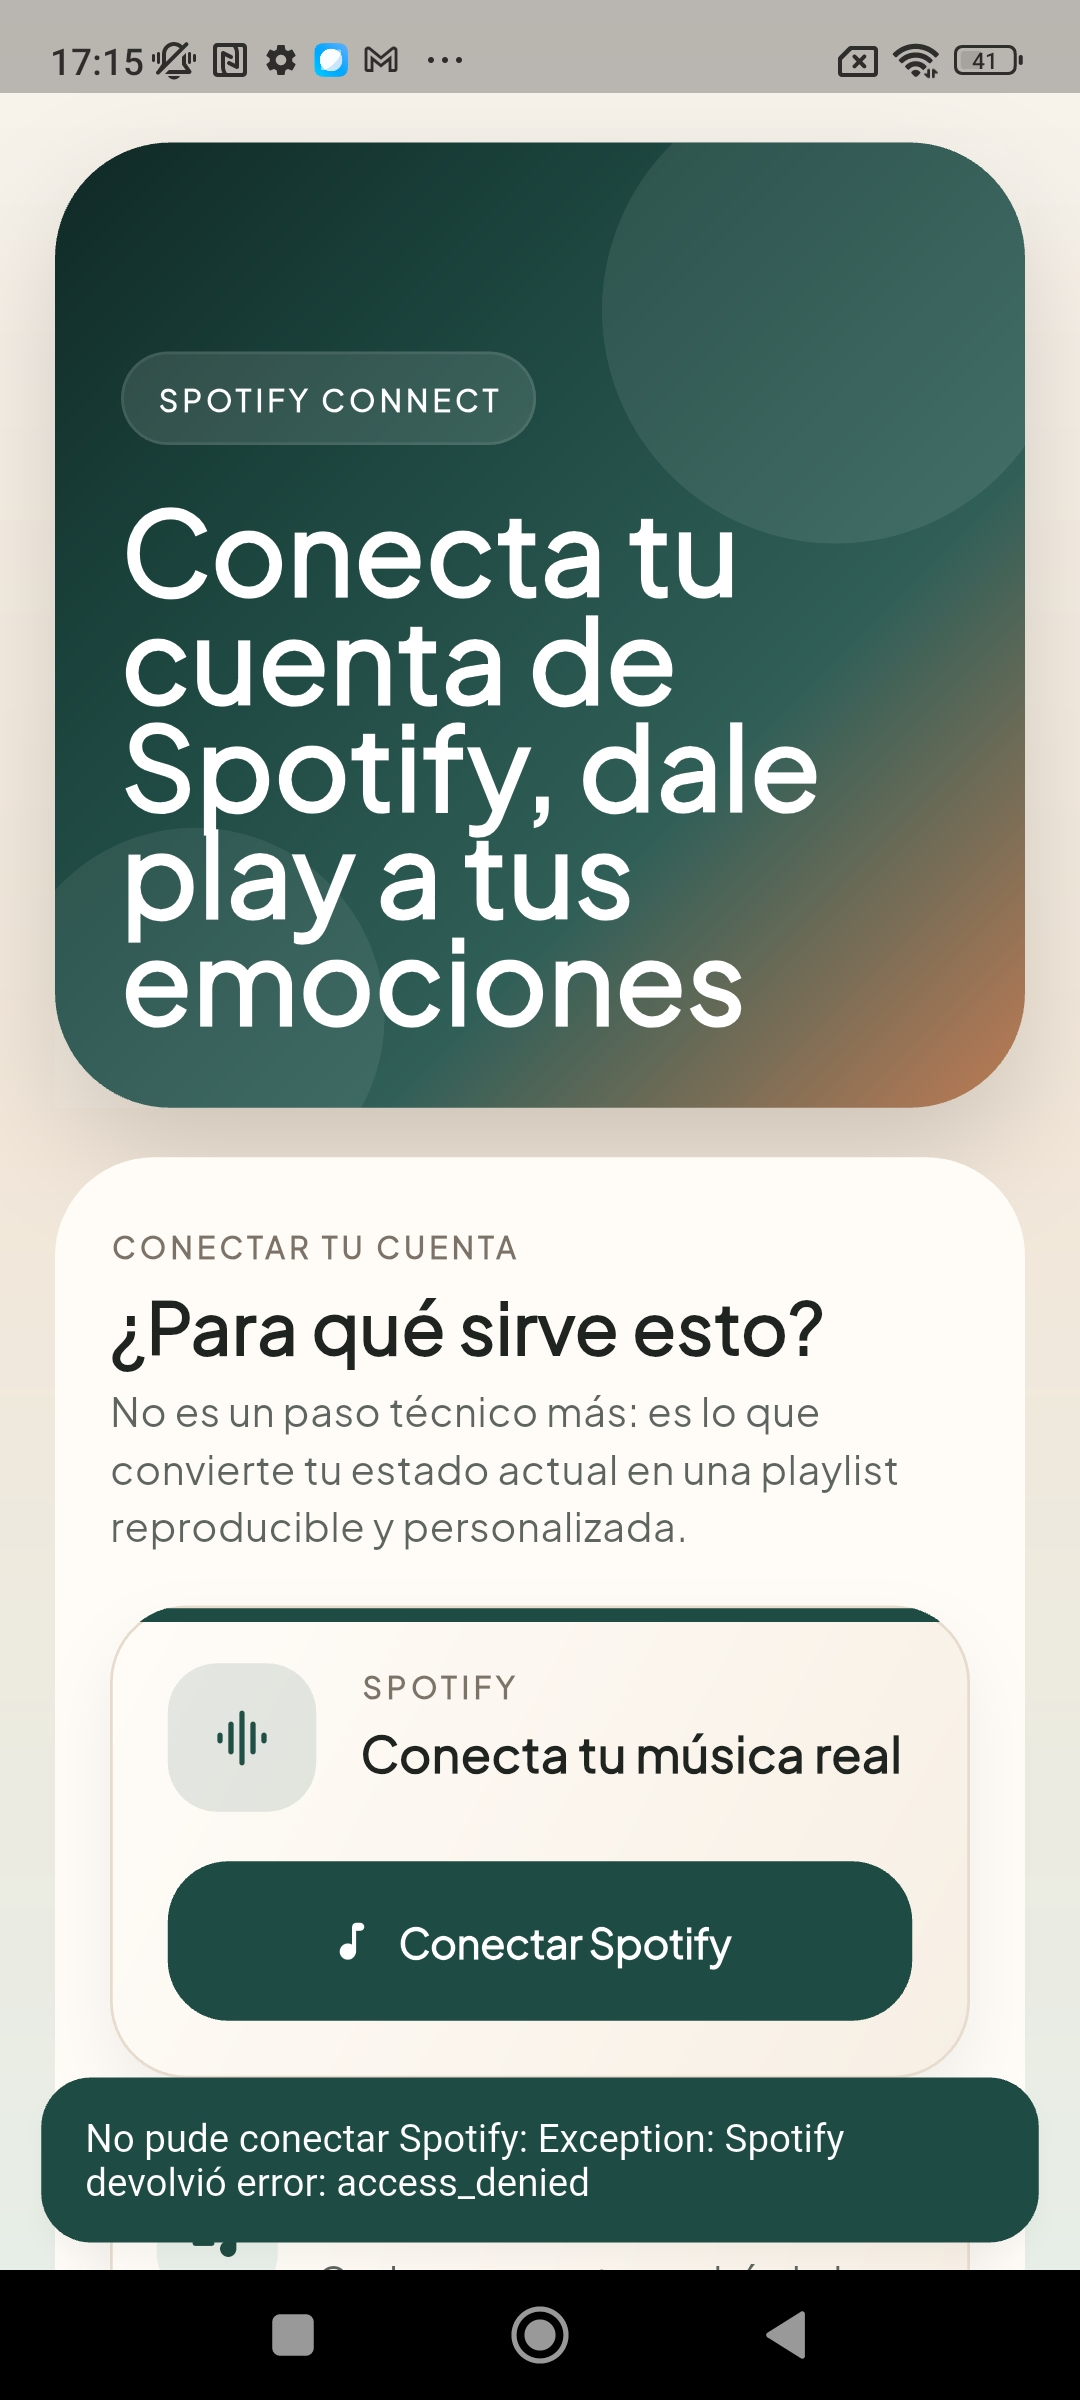
\includegraphics[width=\linewidth]{Imagenes/manual_errores/Screenshot_2026-05-26-17-15-35-245_com.example.harmonyhub.jpg}
    \end{minipage}
    \caption{Dos fallos posibles durante la conexión con Spotify: a la
    izquierda, error de comunicación con el backend local; a la derecha,
    cancelación o denegación del permiso por parte de Spotify.}
    \label{fig:manual_errores_spotify}
\end{figure}

La figura~\ref{fig:manual_errores_spotify} reúne dos casos distintos. En la
primera imagen, Harmony Hub no puede alcanzar el backend y por eso falla el
inicio del flujo OAuth. En una demostración real, esta situación suele
corregirse comprobando que el backend está activo y accesible desde la misma
red que el móvil. En la segunda imagen, el backend sí responde, pero Spotify
devuelve \texttt{access\_denied}; esto significa que la autorización fue
cancelada o rechazada y basta con volver a iniciar la conexión y aceptar el
permiso.

\begin{figure}[htbp]
    \centering
    \begin{minipage}{0.47\textwidth}
        \centering
        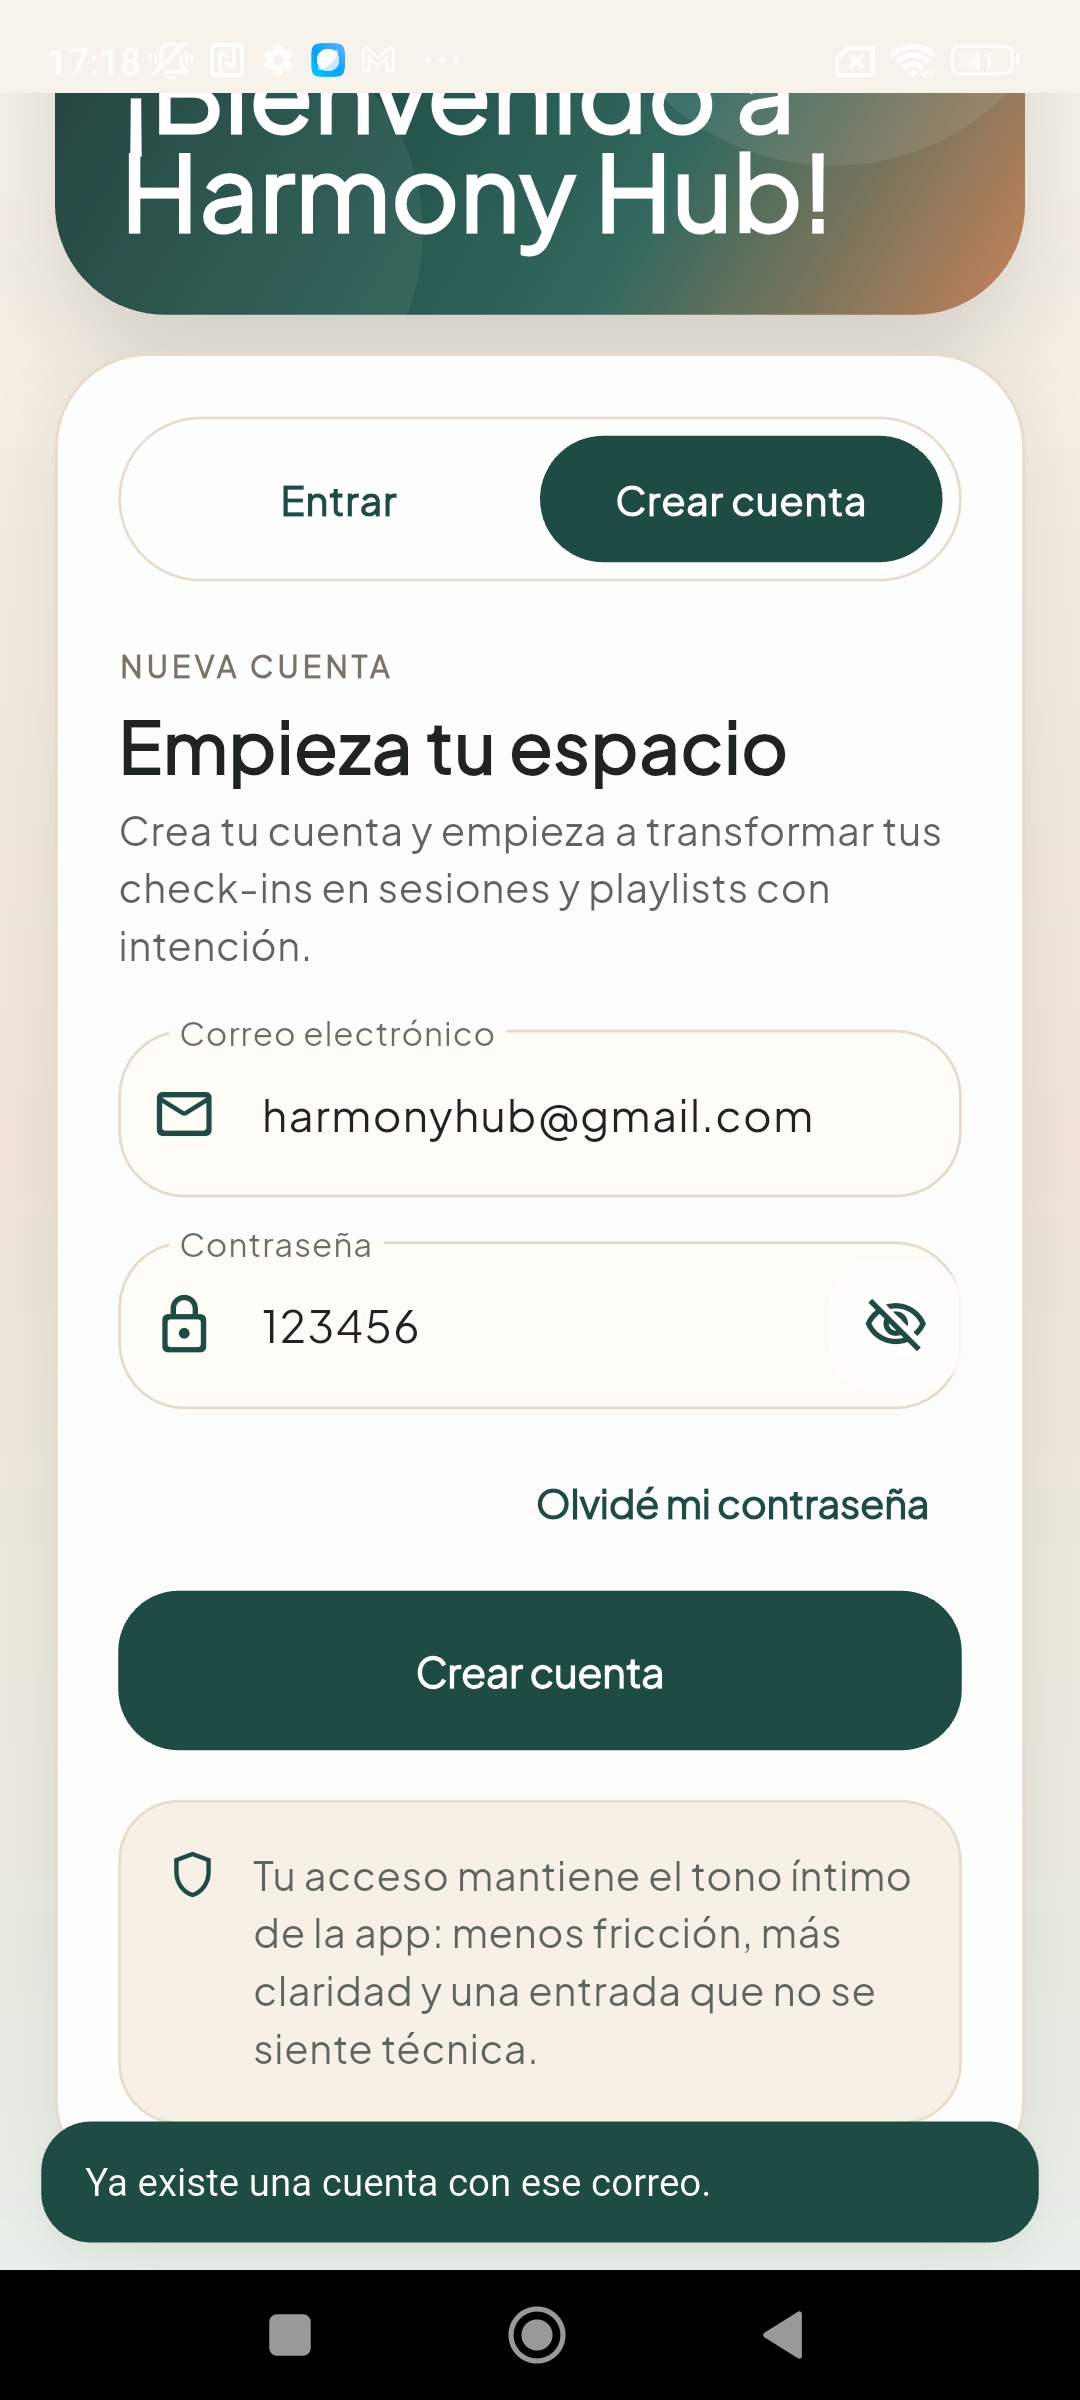
\includegraphics[width=\linewidth]{Imagenes/manual_errores/Screenshot_2026-05-26-17-18-25-628_com.example.harmonyhub.jpg}
    \end{minipage}
    \hfill
    \begin{minipage}{0.47\textwidth}
        \centering
        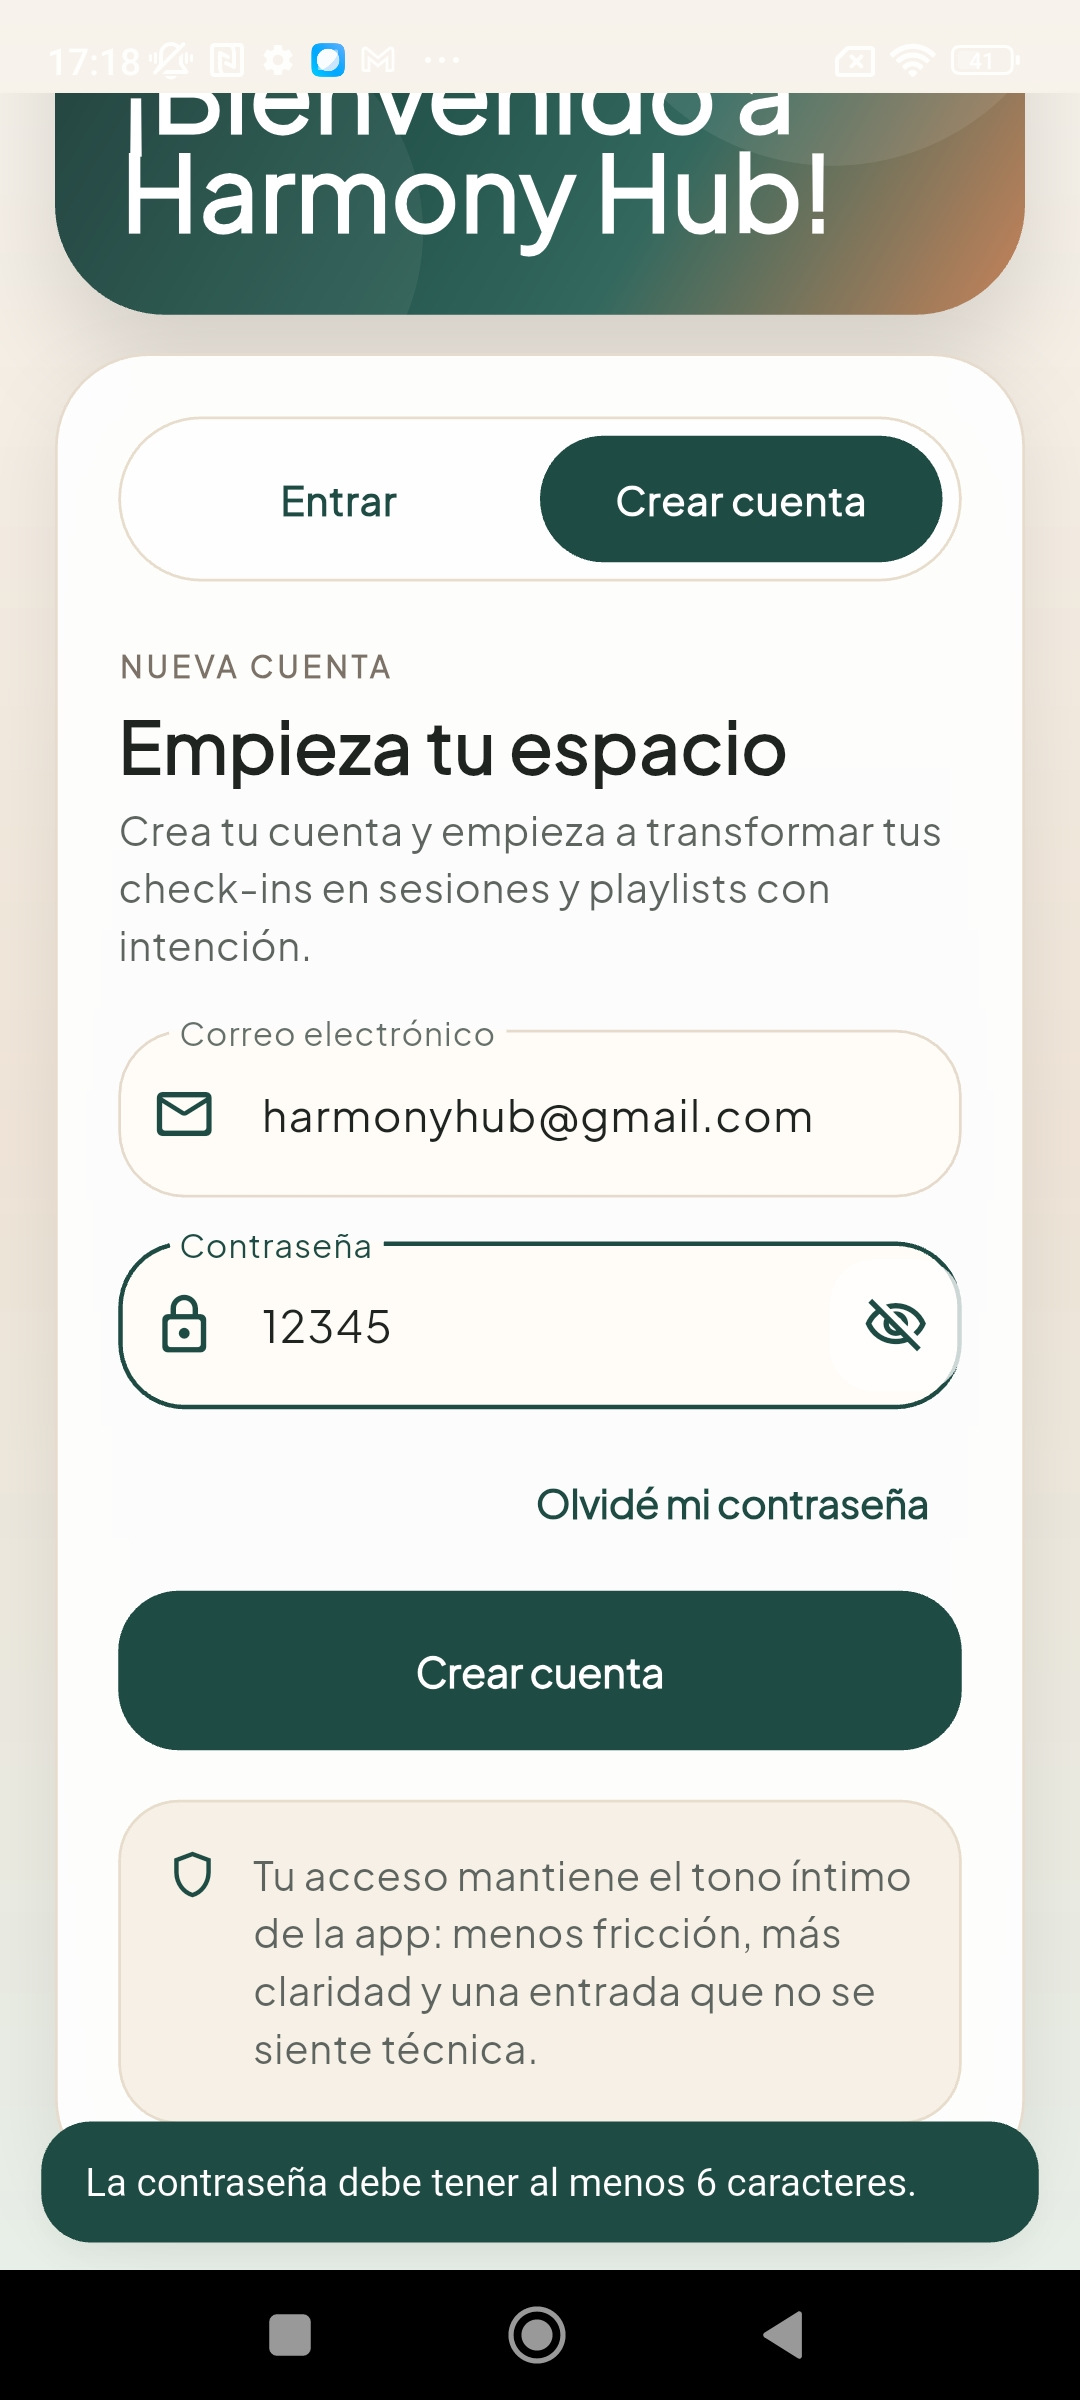
\includegraphics[width=\linewidth]{Imagenes/manual_errores/Screenshot_2026-05-26-17-18-40-964_com.example.harmonyhub.jpg}
    \end{minipage}
    \caption{Validaciones inmediatas del bloque de autenticación: cuenta ya
    existente y contraseña demasiado corta.}
    \label{fig:manual_errores_auth}
\end{figure}

La figura~\ref{fig:manual_errores_auth} muestra dos validaciones sencillas pero
útiles de cara a la experiencia de usuario. La primera evita crear una cuenta
duplicada con un correo que ya existe. La segunda recuerda que la contraseña
debe cumplir una longitud mínima antes de continuar. Ambas validaciones ayudan
a prevenir errores de entrada sin esperar a fases posteriores del flujo.

\begin{figure}[htbp]
    \centering
    \begin{minipage}{0.52\textwidth}
        \centering
        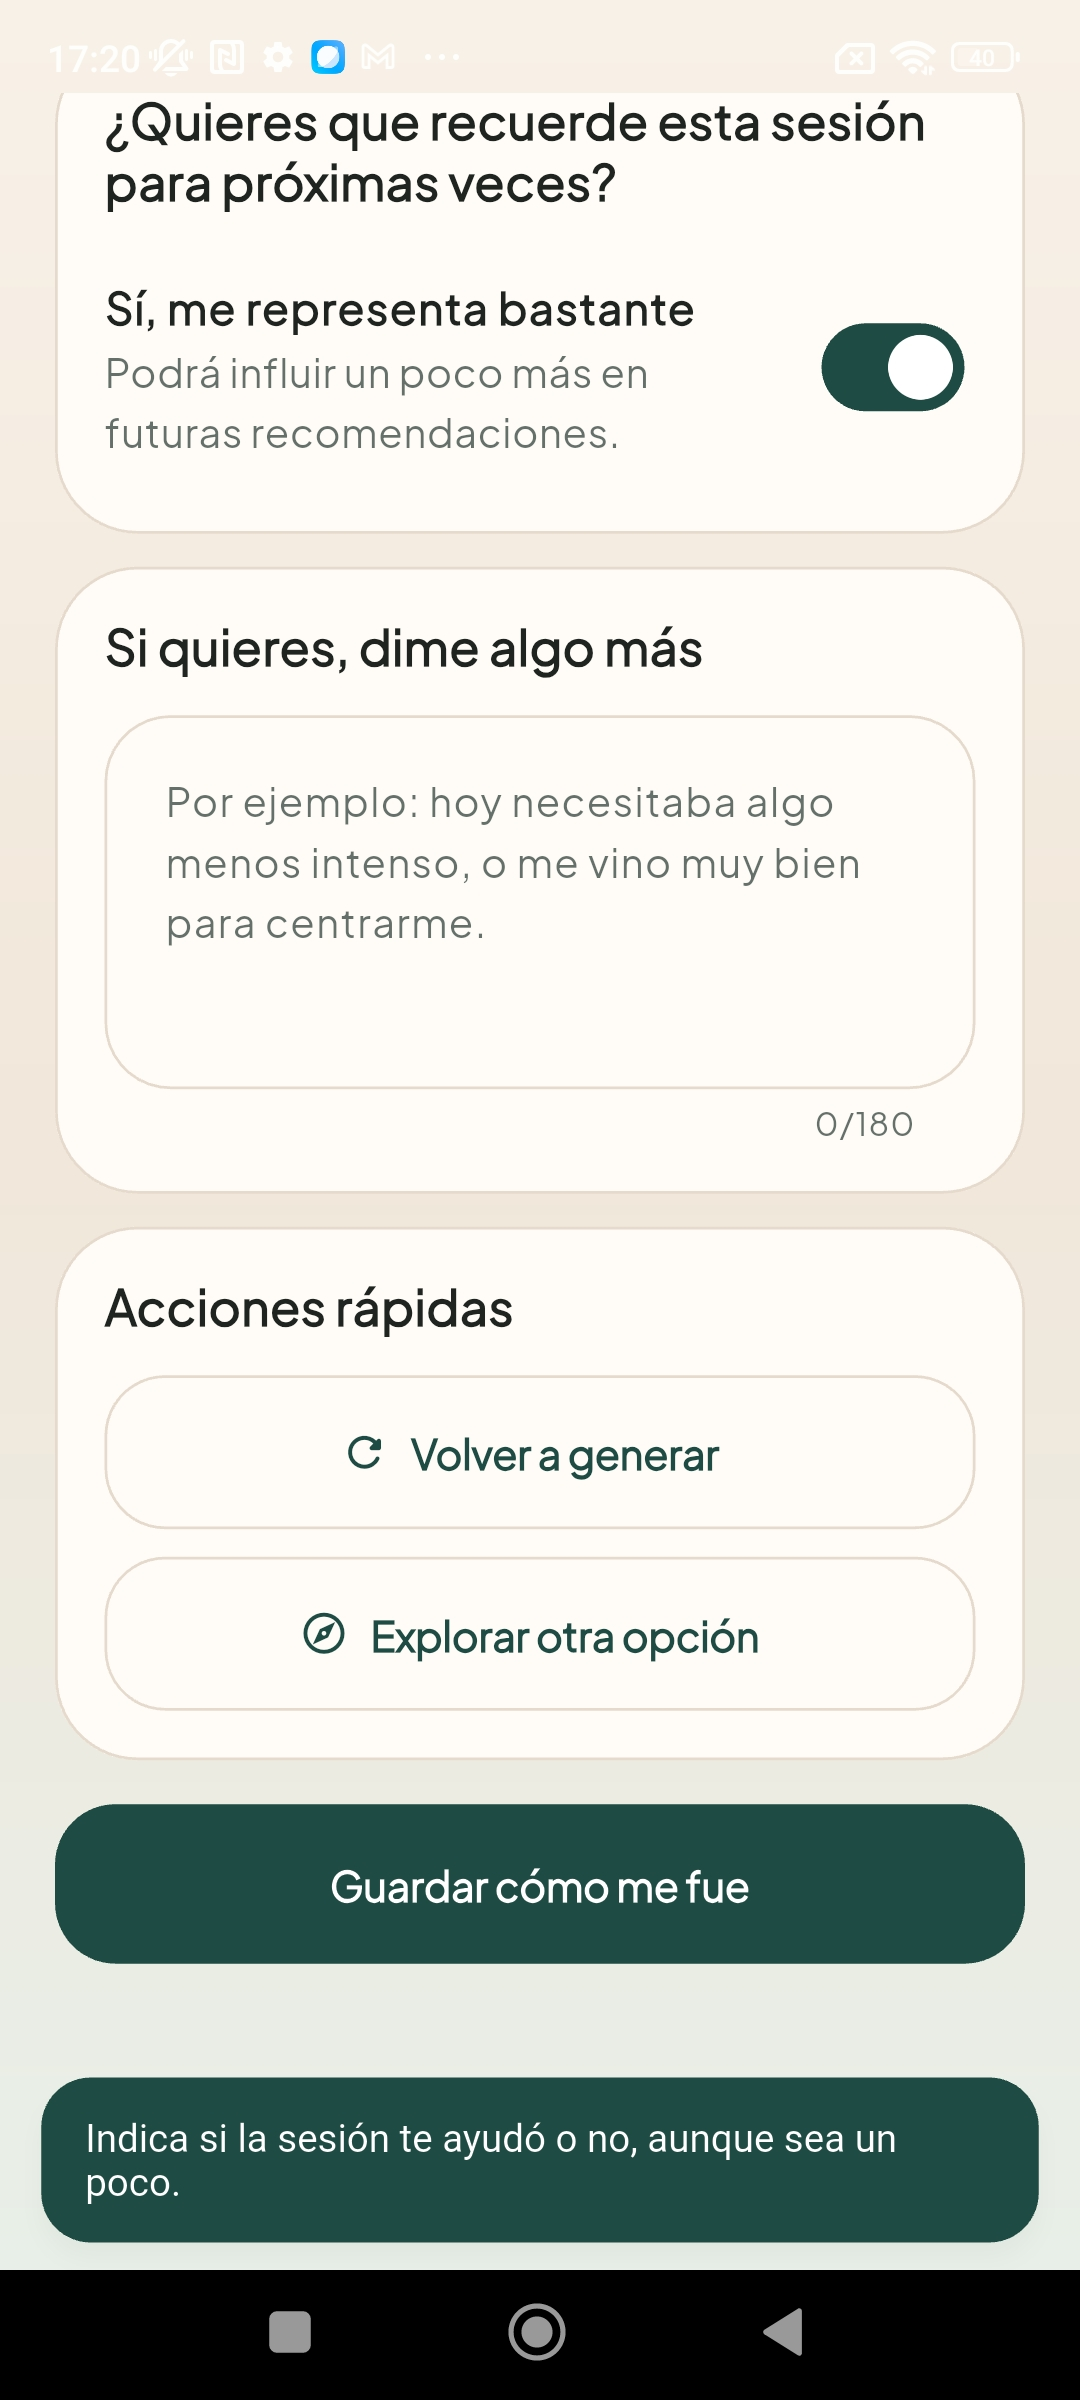
\includegraphics[width=\linewidth]{Imagenes/manual_errores/Screenshot_2026-05-26-17-20-39-922_com.example.harmonyhub.jpg}
    \end{minipage}
    \caption{Validación en la pantalla de feedback cuando se intenta guardar la
    sesión sin indicar todavía si la recomendación ayudó o no.}
    \label{fig:manual_error_feedback}
\end{figure}

Por último, la figura~\ref{fig:manual_error_feedback} refleja un caso ligado al
aprendizaje posterior del sistema. Antes de guardar el cierre de sesión,
Harmony Hub exige que la persona usuaria indique si la experiencia le ayudó al
menos un poco. Esta comprobación tiene una doble utilidad: evita registros
incompletos y garantiza que el backend solo reciba feedback interpretable para
seguir ajustando el perfil aprendido y el componente supervisado.

\section{Funcionalidades principales}
\label{sec:manual_usuario_funcionalidades}

\subsection*{Check-in contextual}

Permite describir el momento actual del usuario mediante una interacción breve.
Es la puerta de entrada del sistema y condiciona la recomendación posterior.

\subsection*{Recomendación de sesión}

La app devuelve un modo sugerido y una explicación funcional del perfil
musical esperado. Esta recomendación puede apoyarse en reglas contextuales y,
cuando existe evidencia suficiente, en aprendizaje acumulado.

\subsection*{Generación de playlist en Spotify}

Si la cuenta está conectada correctamente, la recomendación puede materializarse
como playlist real dentro de Spotify. La aplicación crea la lista y enlaza su
identificador con la sesión correspondiente.

\subsection*{Historial}

El usuario puede revisar sesiones anteriores, playlists generadas y parte de la
trazabilidad funcional acumulada.

\begin{figure}[htbp]
    \centering
    \begin{minipage}{0.47\textwidth}
        \centering
        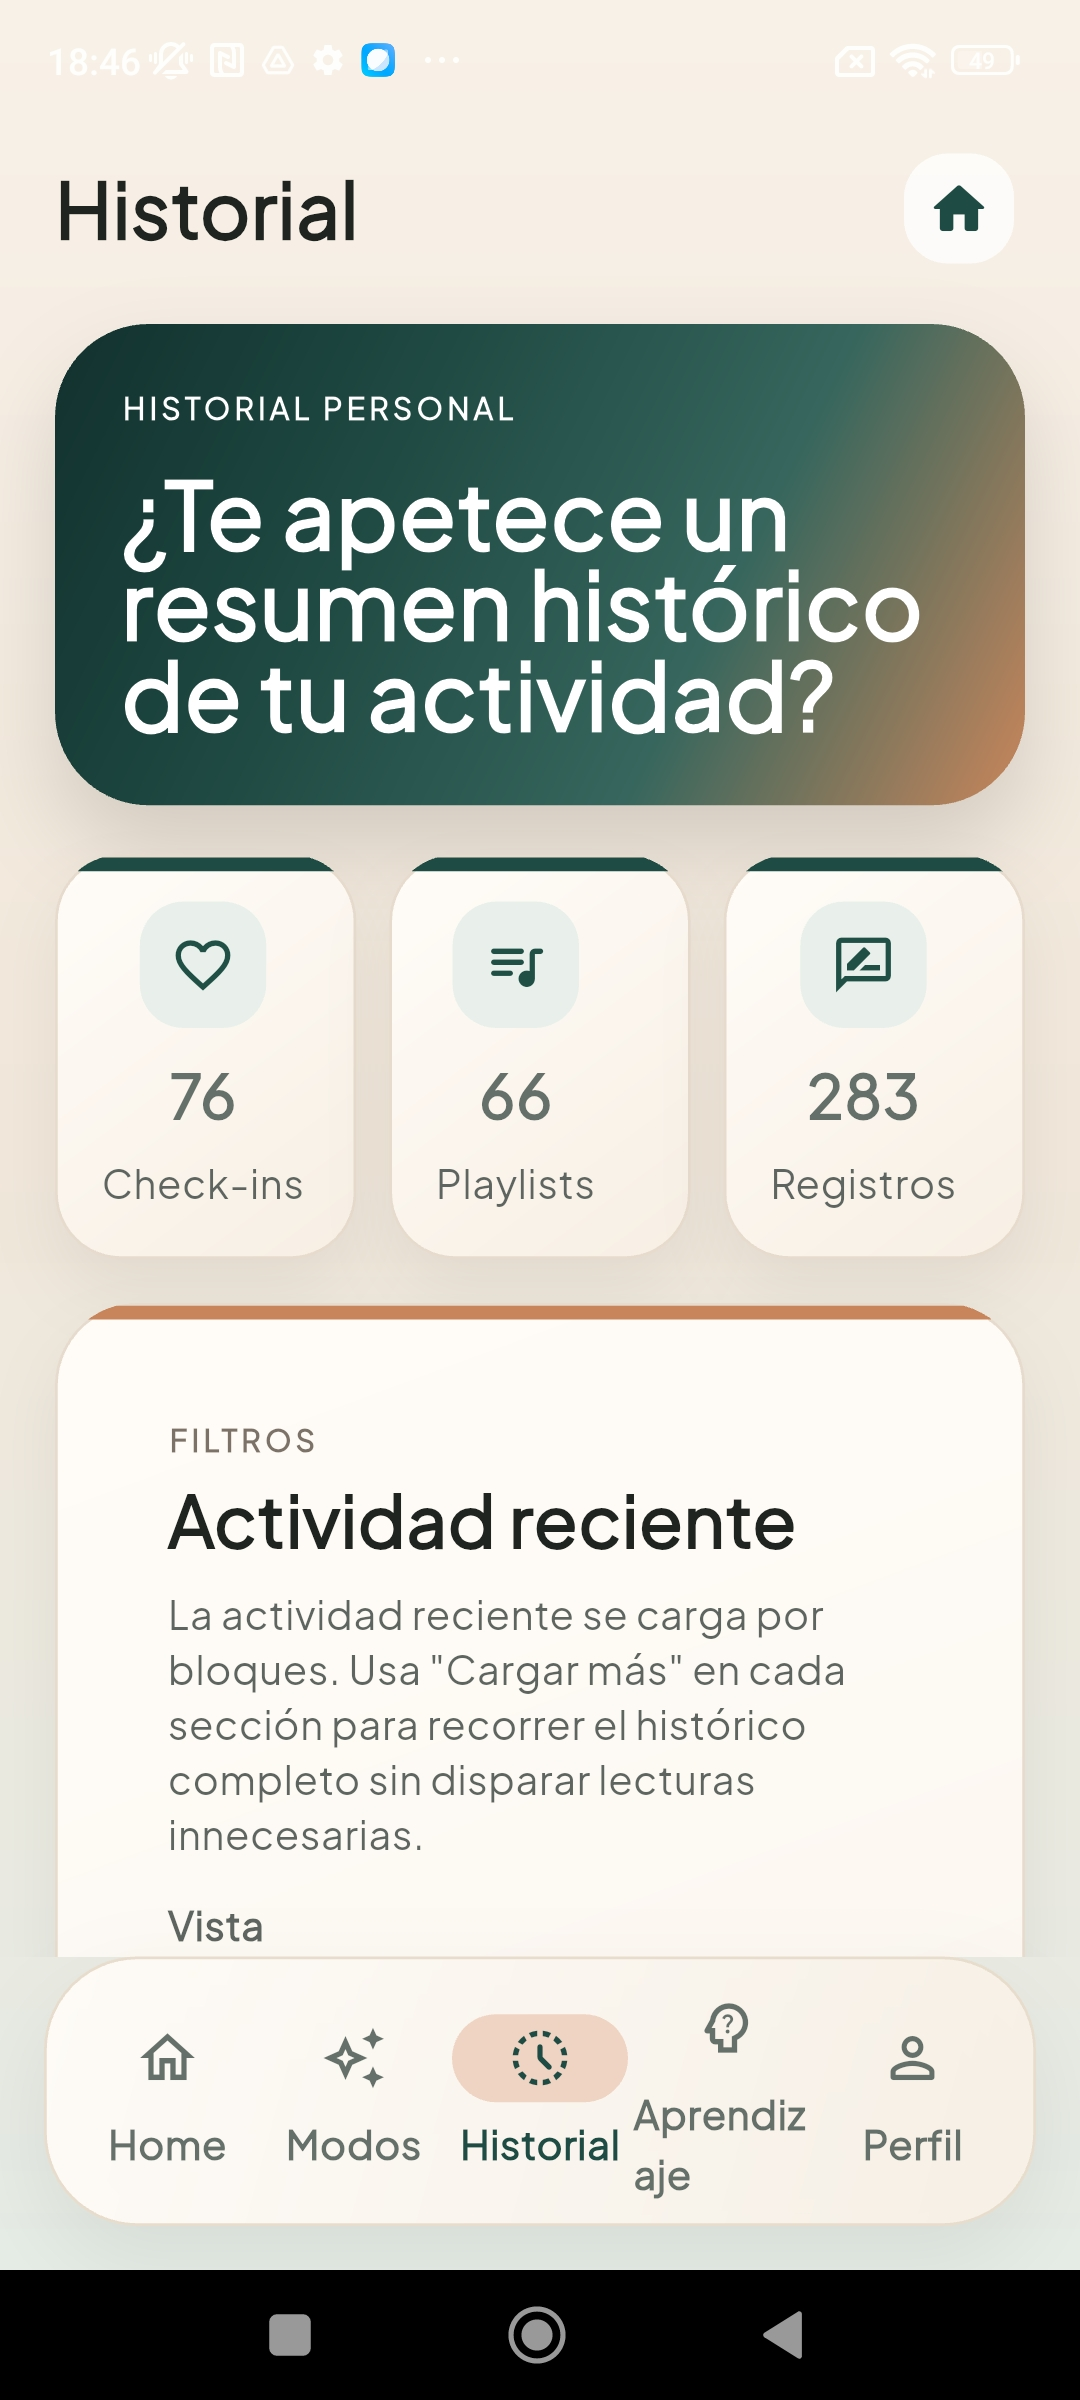
\includegraphics[width=\linewidth]{Imagenes/manual_app/Screenshot_2026-05-25-18-46-30-561_com.example.harmonyhub.jpg}
    \end{minipage}
    \hfill
    \begin{minipage}{0.47\textwidth}
        \centering
        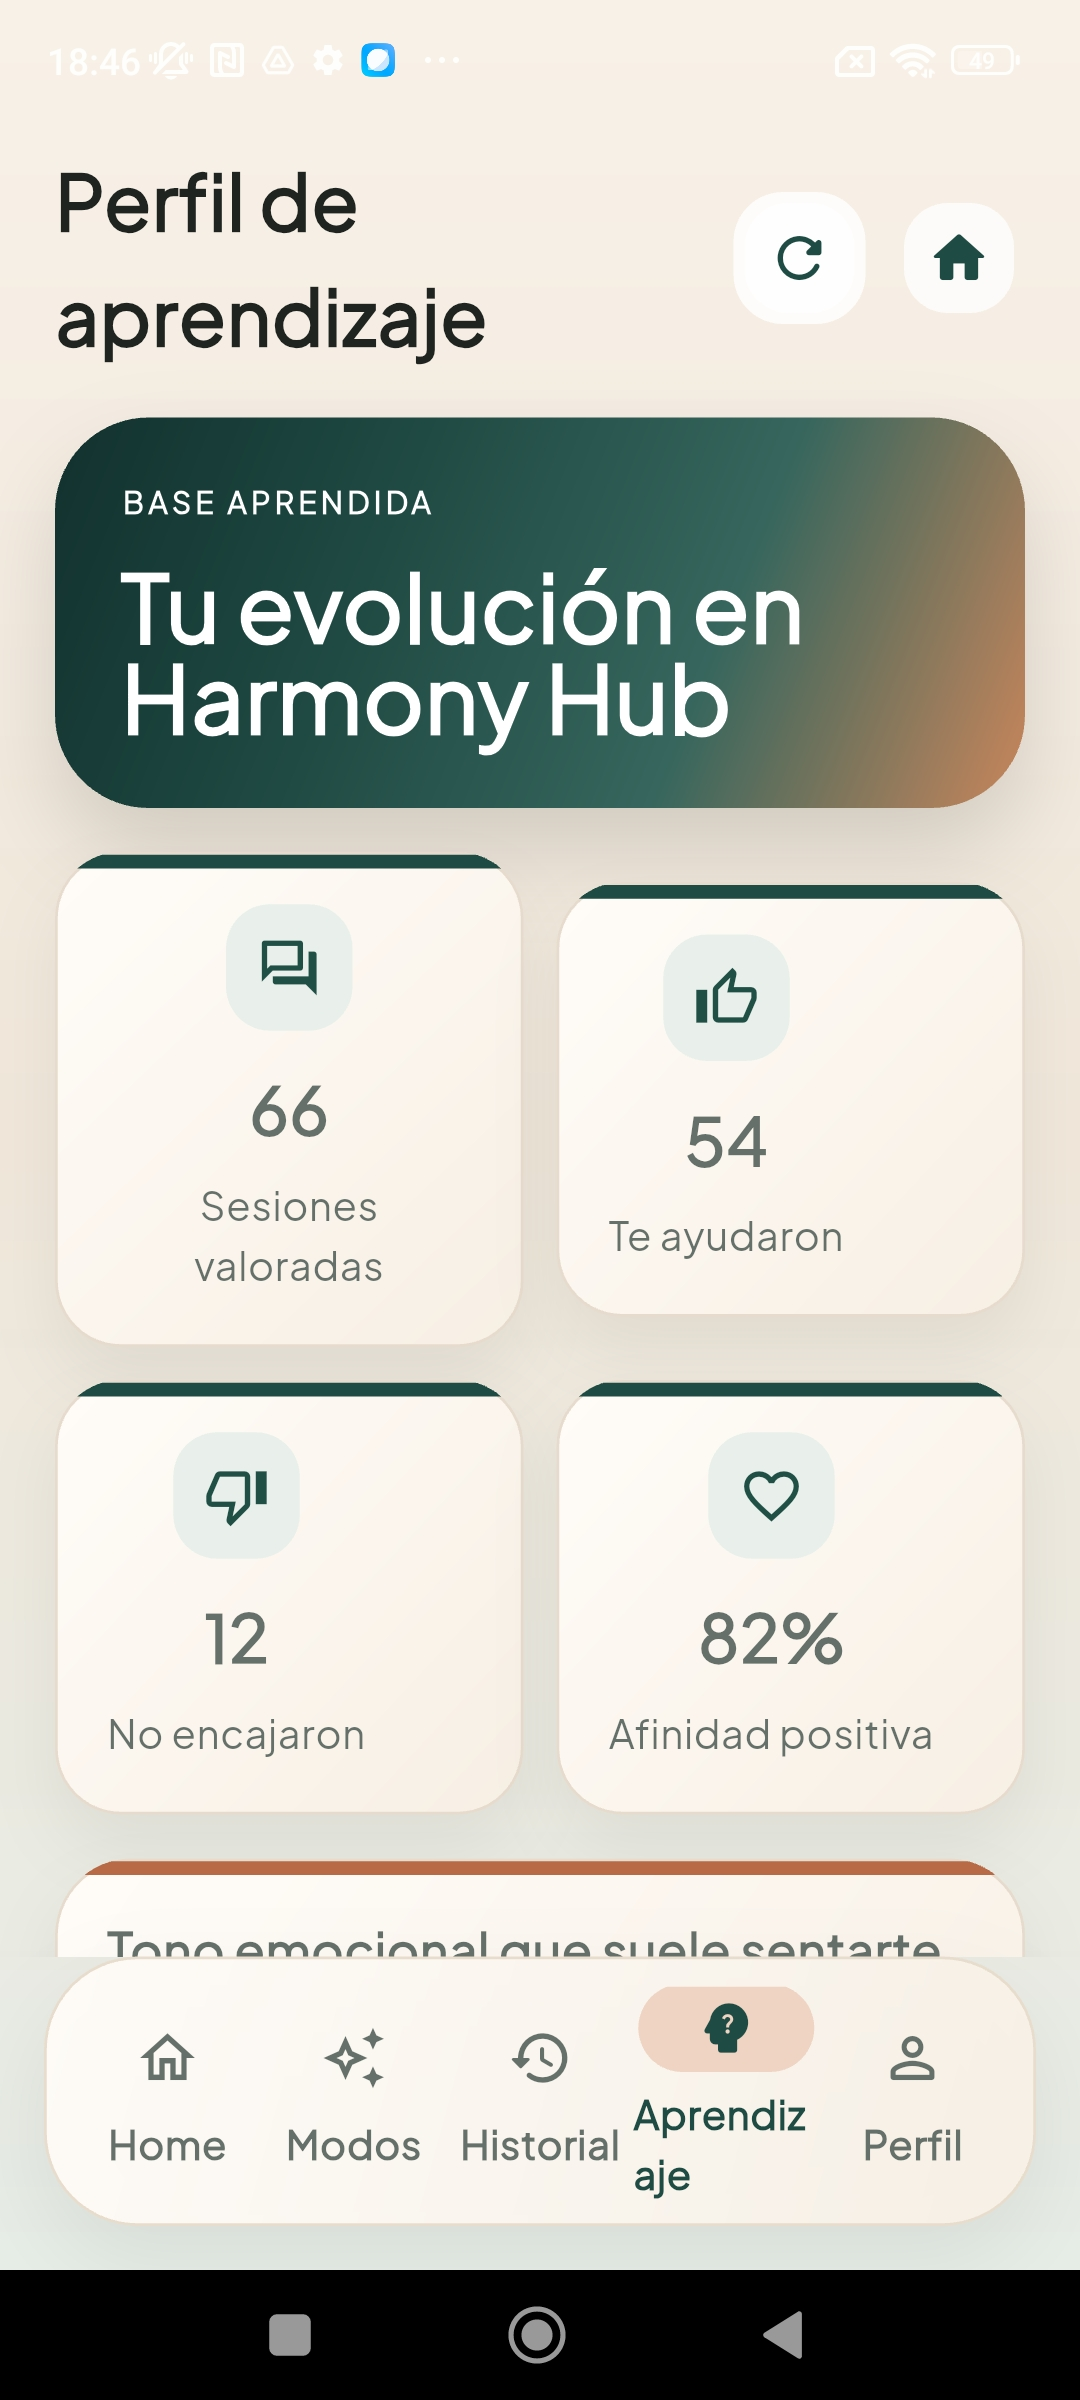
\includegraphics[width=\linewidth]{Imagenes/manual_app/Screenshot_2026-05-25-18-46-35-030_com.example.harmonyhub.jpg}
    \end{minipage}
    \caption{Bloques secundarios accesibles desde la navegación: modos
    guardados o accesos recurrentes, a la izquierda, e historial personal, a la
    derecha.}
    \label{fig:manual_modos_historial}
\end{figure}

La navegación inferior permite acceder a bloques complementarios sin romper el
flujo principal. En \textit{Modos} se muestran modos guardados, accesos rápidos
o rutas útiles para situaciones recurrentes; en \textit{Historial} se resume la
actividad previa del usuario y se facilita la revisión de sesiones ya
realizadas.

\subsection*{Aprendizaje personal}

La app muestra información resumida sobre el aprendizaje del sistema respecto a
las preferencias del usuario, incluyendo pesos contextuales y estables cuando
existe suficiente actividad acumulada.

\begin{figure}[htbp]
    \centering
    \begin{minipage}{0.31\textwidth}
        \centering
        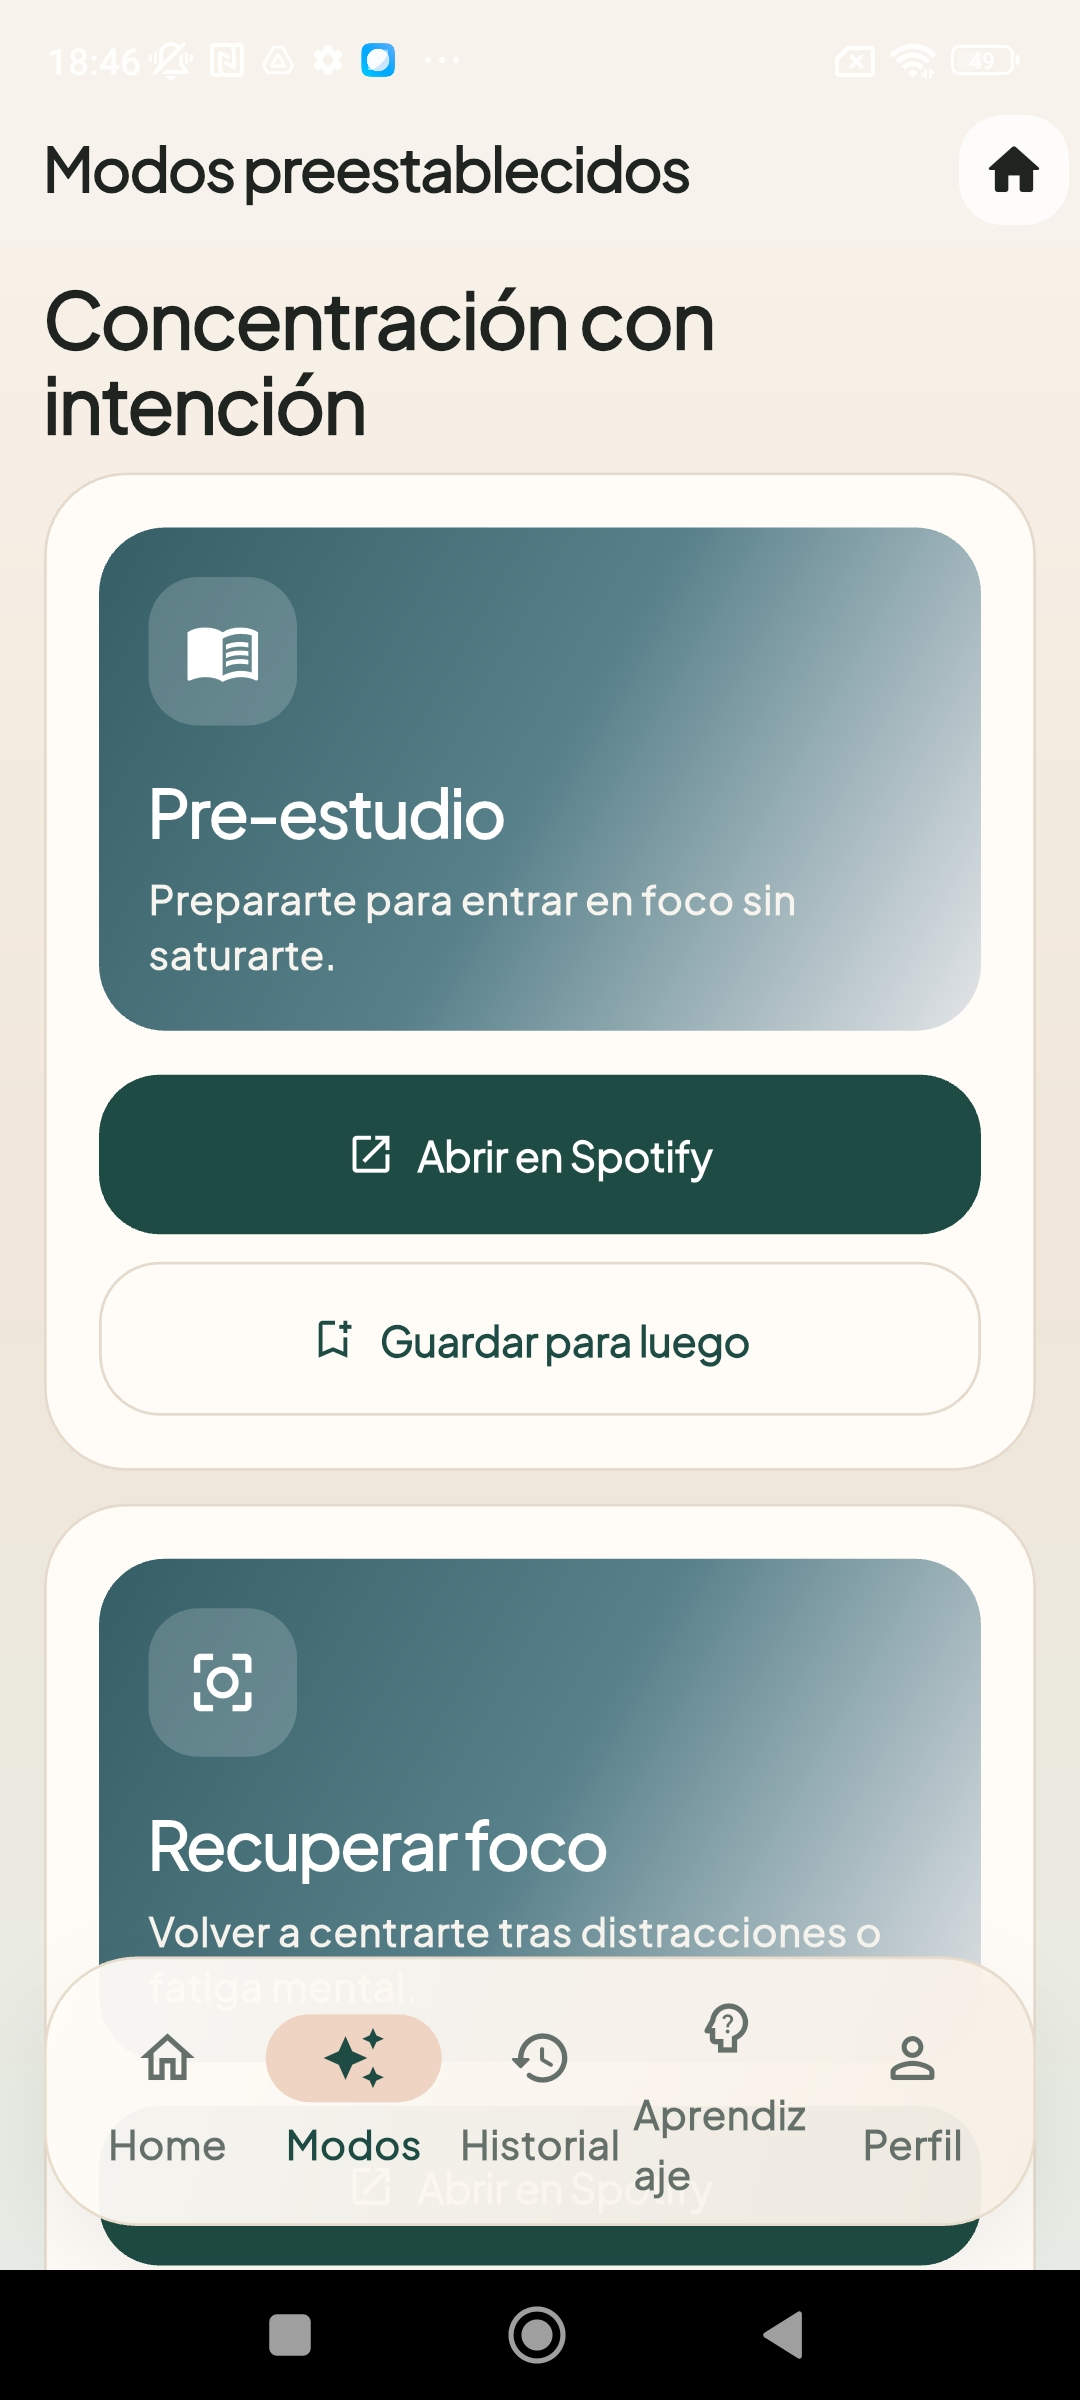
\includegraphics[width=\linewidth]{Imagenes/manual_app/Screenshot_2026-05-25-18-46-24-532_com.example.harmonyhub.jpg}
    \end{minipage}
    \hfill
    \begin{minipage}{0.31\textwidth}
        \centering
        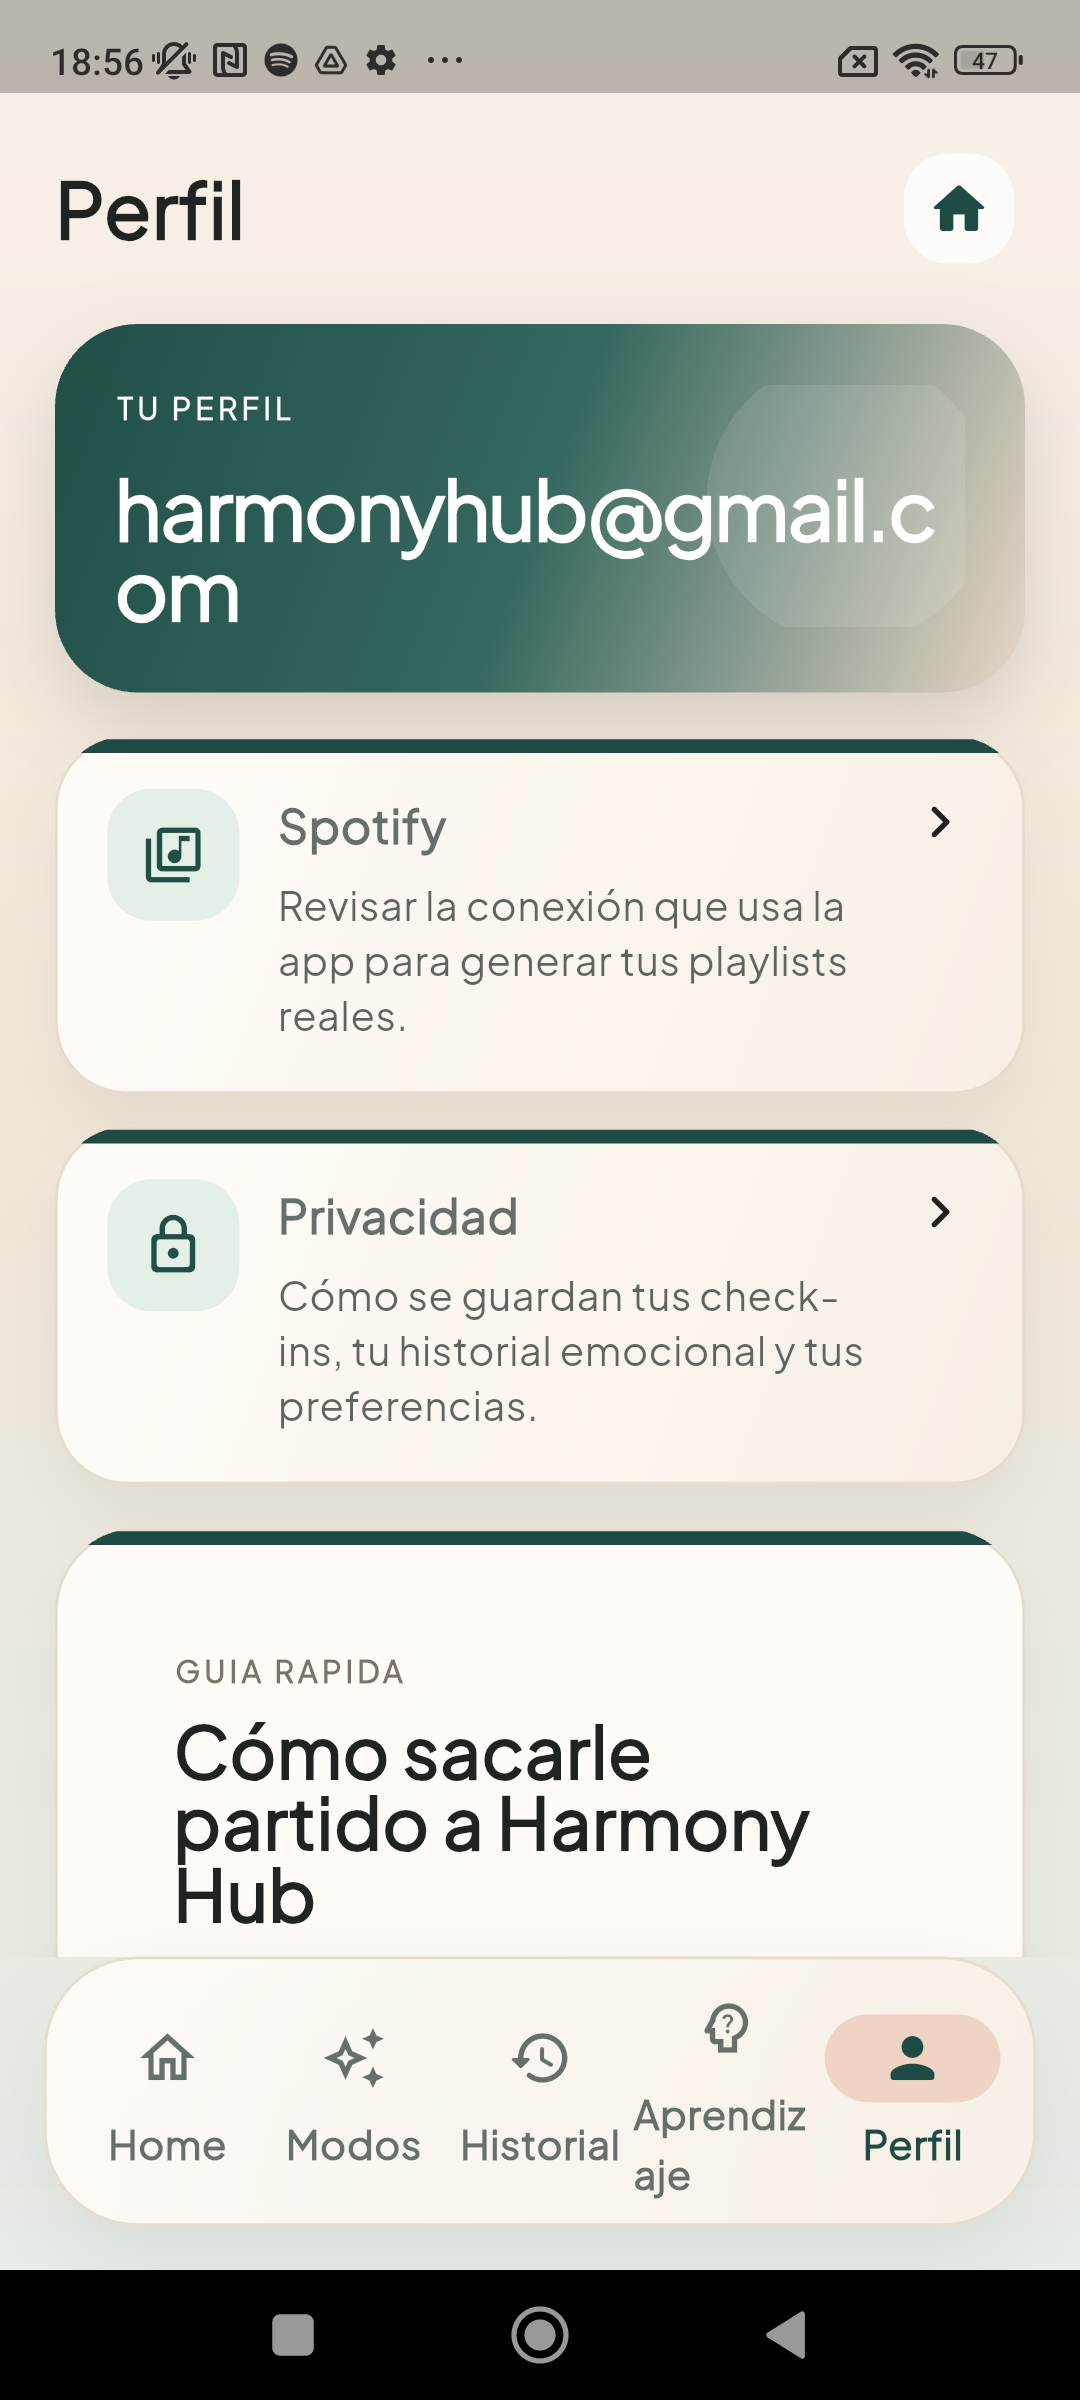
\includegraphics[width=\linewidth]{Imagenes/manual_app/Screenshot_2026-05-25-18-56-50-176_com.example.harmonyhub.jpg}
    \end{minipage}
    \hfill
    \begin{minipage}{0.31\textwidth}
        \centering
        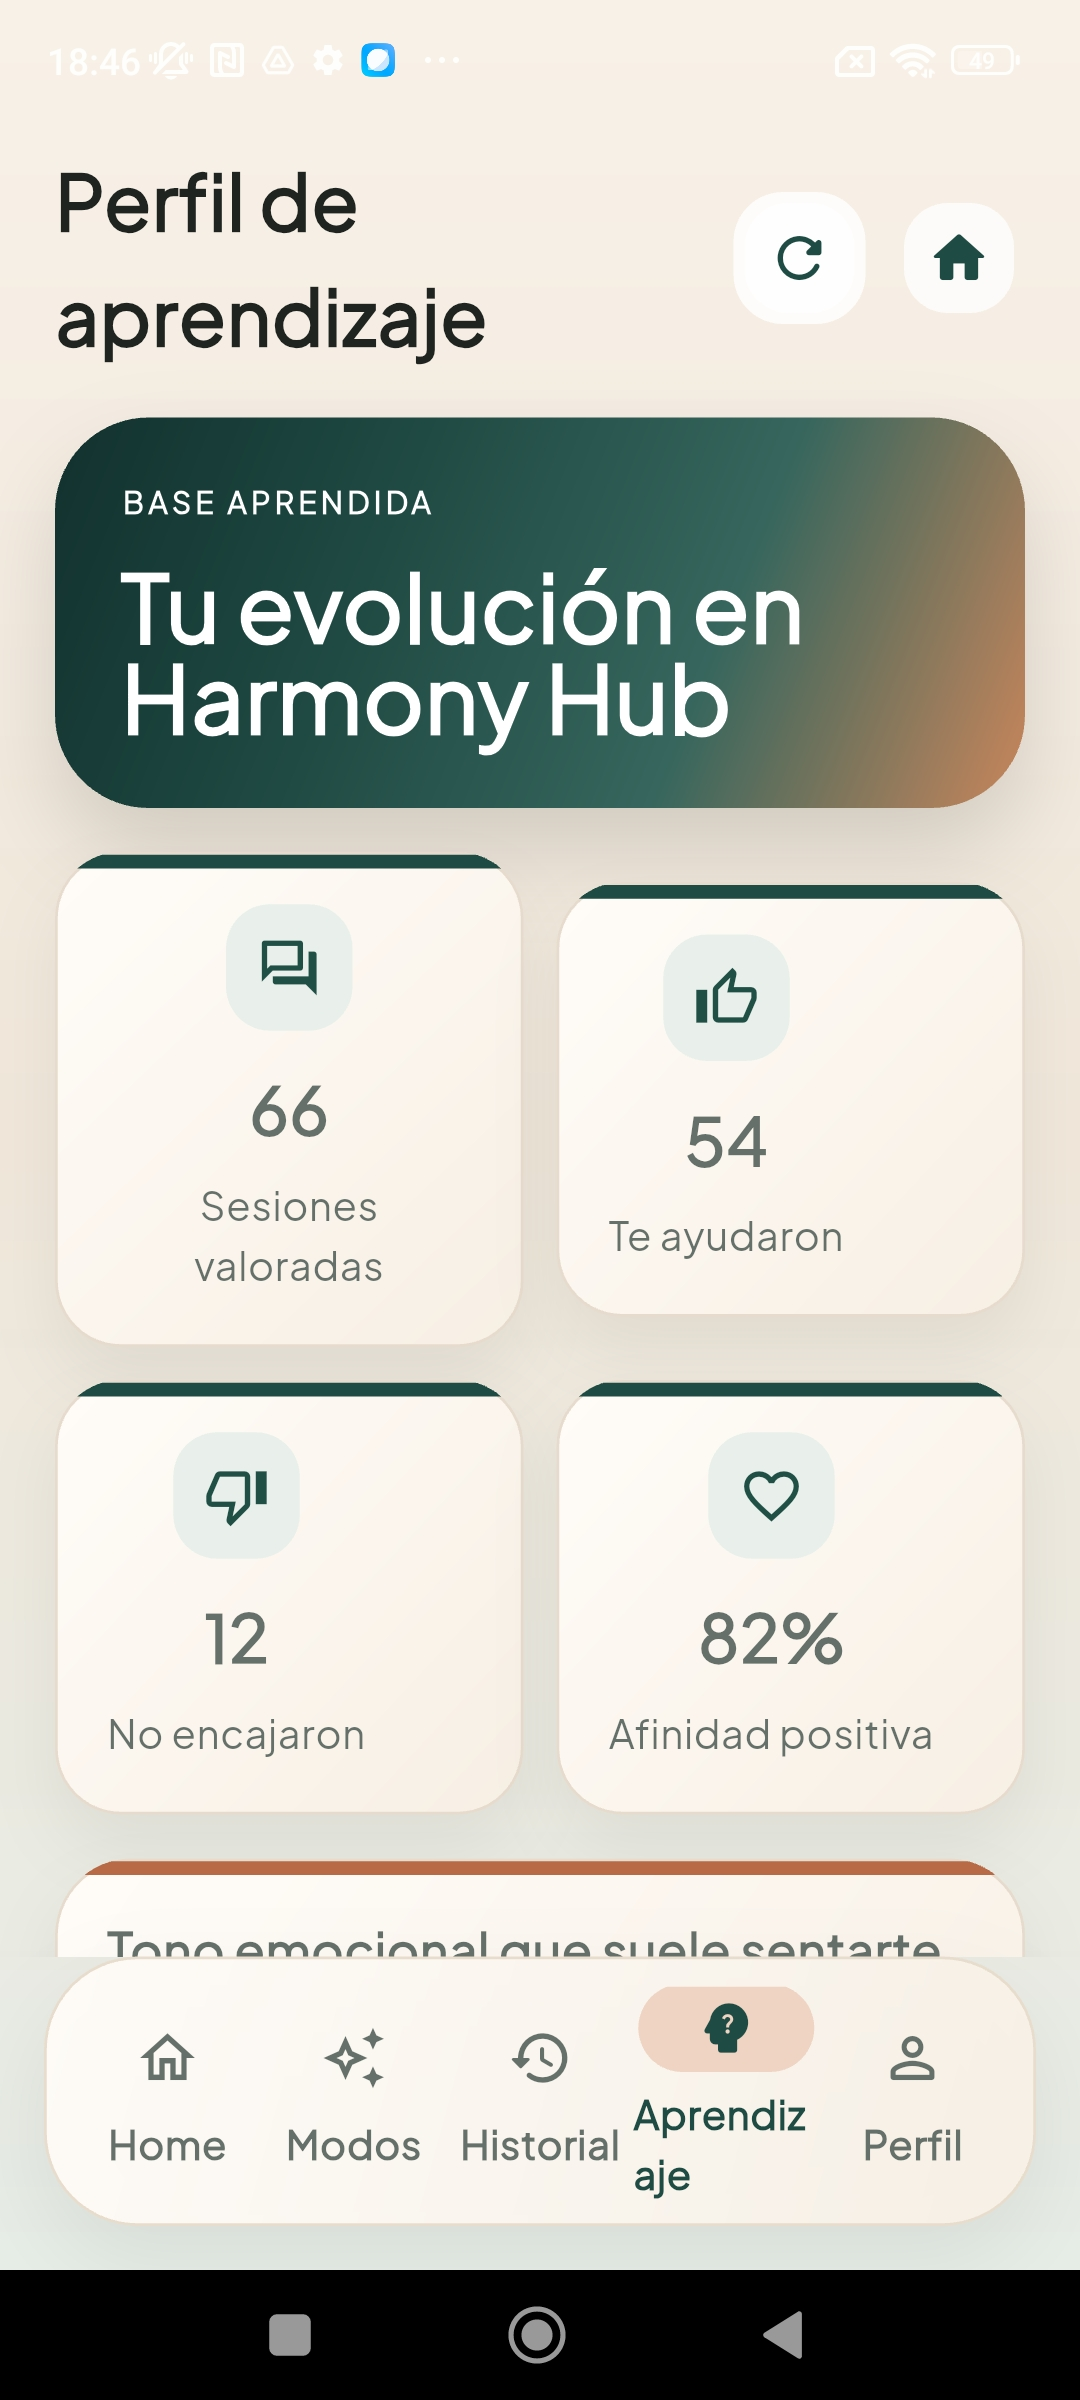
\includegraphics[width=\linewidth]{Imagenes/manual_app/Screenshot_2026-05-25-18-46-35-030_com.example.harmonyhub.jpg}
    \end{minipage}
    \caption{Pantallas de aprendizaje, perfil y modos guardados o accesos
    recurrentes entre secciones.}
    \label{fig:manual_aprendizaje_perfil}
\end{figure}

En \textit{Aprendizaje} se muestran indicadores resumidos sobre sesiones
valoradas, afinidad positiva y otras señales útiles para entender si el sistema
ya dispone de una base suficiente para personalizar mejor. En \textit{Perfil}
se agrupan opciones relacionadas con Spotify, privacidad y ayuda rápida de uso.
La tercera captura muestra el bloque de \textit{Modos}, donde aparecen modos
guardados o accesos recurrentes para reutilizar rutas funcionales frecuentes.

\subsection*{Modos guardados}

Para situaciones recurrentes, el sistema permite conservar accesos o modos
rápidos, de forma que no sea necesario repetir siempre la misma interacción
desde cero.

\section{Resolución de problemas frecuentes}
\label{sec:manual_usuario_problemas}

\subsection*{No se puede conectar Spotify}

Comprobar que:

\begin{itemize}
    \item la cuenta de Spotify ha aceptado la autorización;
    \item la redirección OAuth está bien configurada;
    \item el backend de demostración está en ejecución y accesible desde la red local;
    \item la conexión de red está disponible.
\end{itemize}

\subsection*{La recomendación se genera, pero la playlist falla}

Esto suele estar relacionado con restricciones externas de Spotify, problemas
temporales de materialización o falta de conectividad con el backend. En ese
caso conviene:

\begin{itemize}
    \item esperar unos minutos si hubo demasiadas búsquedas seguidas;
    \item volver a intentar la generación más tarde;
    \item comprobar que el móvil mantiene conectividad con la red de la demostración;
    \item comprobar que la cuenta de Spotify sigue conectada.
\end{itemize}

\subsection*{El entorno no se analiza}

Si no se ha concedido permiso de micrófono, la app seguirá funcionando, pero
sin apoyo acústico del entorno. Basta con conceder permiso cuando se quiera
utilizar esa funcionalidad.

\subsection*{No se aprecia aprendizaje todavía}

El sistema puede funcionar desde la primera sesión, pero la personalización
aprendida necesita varias sesiones cerradas con feedback. Si el usuario todavía
no ve cambios claros, conviene seguir completando sesiones y aportar feedback
útil al final de cada una.

\chapter{Manual de código y repositorio}
\label{anexo:manual_codigo}

Este anexo actúa únicamente como punto de referencia para el acceso al código
fuente del proyecto. Harmony Hub se entrega como repositorio versionado, con la
aplicación móvil, el backend, la documentación académica y los artefactos de
validación integrados en una única estructura de trabajo.

La versión pública y consultable del proyecto se encuentra en:

\begin{center}
\url{https://github.com/i22remua/THE-HARMONY-HUB}
\end{center}

Desde ese repositorio pueden revisarse la organización del cliente Flutter, la
implementación del backend FastAPI, la integración con Spotify, el catálogo
musical estructurado, el componente de aprendizaje y la propia memoria del
TFG.

\section*{Puertas de calidad del modelo supervisado}

Para evitar que el componente de aprendizaje actúe con evidencia insuficiente,
Harmony Hub incorpora una política explícita de puertas de calidad antes de
permitir que el modelo reordene candidatos de sesión. Esta explicación resume
lo desarrollado en el diseño de la solución y facilita localizarlo en el código
y en los artefactos de auditoría.

En primer lugar, se aplica una \textbf{puerta de datos}. El modelo solo puede
considerarse operativo cuando existe un mínimo de ejemplos totales y una
cobertura mínima por clase. En términos prácticos, esto significa que no basta
con acumular muchas sesiones, sino que deben existir suficientes casos útiles y
no útiles para que el clasificador vea ambos comportamientos. En la
implementación actual se exige \texttt{total\_examples >= 40} y al menos
\texttt{8} ejemplos por clase.

En segundo lugar, cuando la distribución lo permite, se utiliza
\textbf{validación cruzada estratificada}. Esta técnica divide el conjunto de
ejemplos en varios pliegues conservando proporciones similares de clases en
cada partición. Su objetivo es reducir el riesgo de considerar válido un modelo
que solo funciona bien en una única separación afortunada de los datos.

Sobre esa validación se calculan varias métricas. La
\textbf{balanced accuracy} mide si el modelo diferencia de forma razonable las
sesiones útiles y las no útiles sin sesgarse hacia la clase mayoritaria. El
\textbf{ROC AUC} mide si el clasificador sabe asignar más probabilidad a los
casos positivos que a los negativos antes incluso de fijar un umbral binario.
La métrica \textbf{F1-score} resume el equilibrio entre precisión y recobrado
de la clase positiva.

Para sintetizar estas señales se utiliza un \textbf{índice compuesto de
calidad}, calculado como:

\begin{center}
\texttt{quality score = (0.45 * balanced accuracy + 0.35 * ROC AUC + 0.20 * F1) * 100}
\end{center}

En la configuración actual, el modelo solo supera la puerta de calidad si
alcanza simultáneamente:

\begin{itemize}
    \item \texttt{balanced accuracy >= 0.45},
    \item \texttt{ROC AUC >= 0.38},
    \item \texttt{quality score >= 49}.
\end{itemize}

Además, incluso cuando el modelo ha sido entrenado y auditado correctamente, su
influencia sobre una recomendación concreta queda condicionada por una
\textbf{puerta de confianza operacional}. Esta última exige que la probabilidad
del mejor candidato supere un umbral mínimo antes de modificar el ranking
heurístico. En el estado actual del proyecto, ese valor operativo aparece
registrado como \texttt{min\_selected\_mode\_probability = 0.14}.

Estas comprobaciones pueden localizarse directamente en los siguientes puntos
del repositorio:

\begin{itemize}
    \item \texttt{backend\_fastapi/app/services/session\_mode\_ml\_service.py}: umbrales operativos y activación del modelo en tiempo de recomendación.
    \item \texttt{backend\_fastapi/app/ml/train\_ranking\_model.py}: entrenamiento, validación cruzada, cálculo de métricas y decisión de paso de puertas.
    \item \texttt{backend\_fastapi/app/ml/models/session\_mode\_model\_audit.json}: evidencia persistida del estado de auditoría y de los umbrales vigentes.
    \item \texttt{backend\_fastapi/app/ml/models/session\_mode\_model\_card.json}: resumen funcional del modelo, su propósito y sus parámetros de operación.
\end{itemize}

Esta política de control tiene una función importante dentro del proyecto: el
aprendizaje no sustituye a la base heurística, sino que solo interviene cuando
dispone de evidencia mínima, calidad suficiente y confianza operacional en el
contexto evaluado.


% Anexos opcionales de la plantilla original. Descomenta solo si los necesitas.
% \input{planos}
% \chapter{Hojas de Características}

% Pages: Es este parámetro se indican cuantas páginas se quieren poner 1 o 1-2, ...
% Angle: A veces es necesario rotar la página --> angle=90
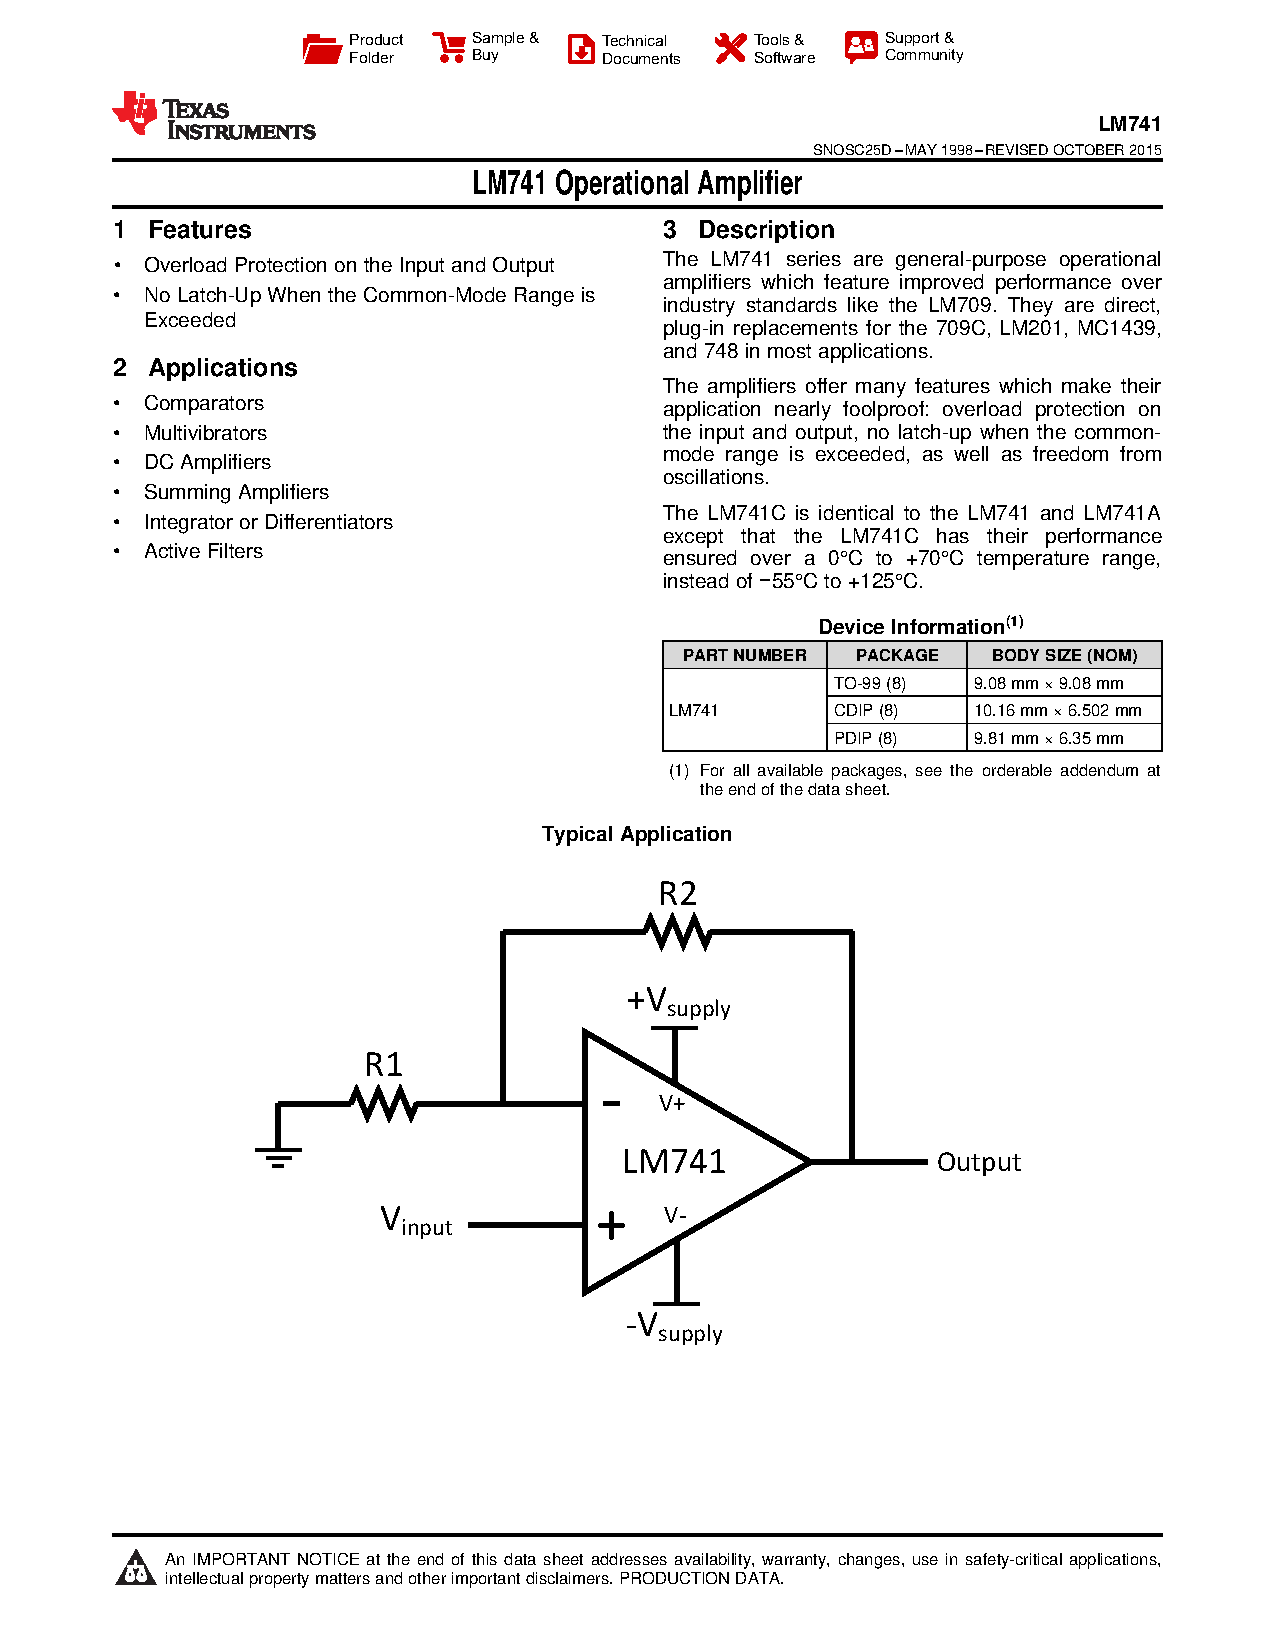
\includepdf[scale=0.7,pages=1,angle=0,pagecommand=\section{Amplificador Operacional 741}\label{hc:ao_741}]{HojasDeCaracteristicas/ejemplo_lm741.pdf}

% Si se ponen varias páginas hay que hacerlo de la siguiente forma:
% Pagina 1
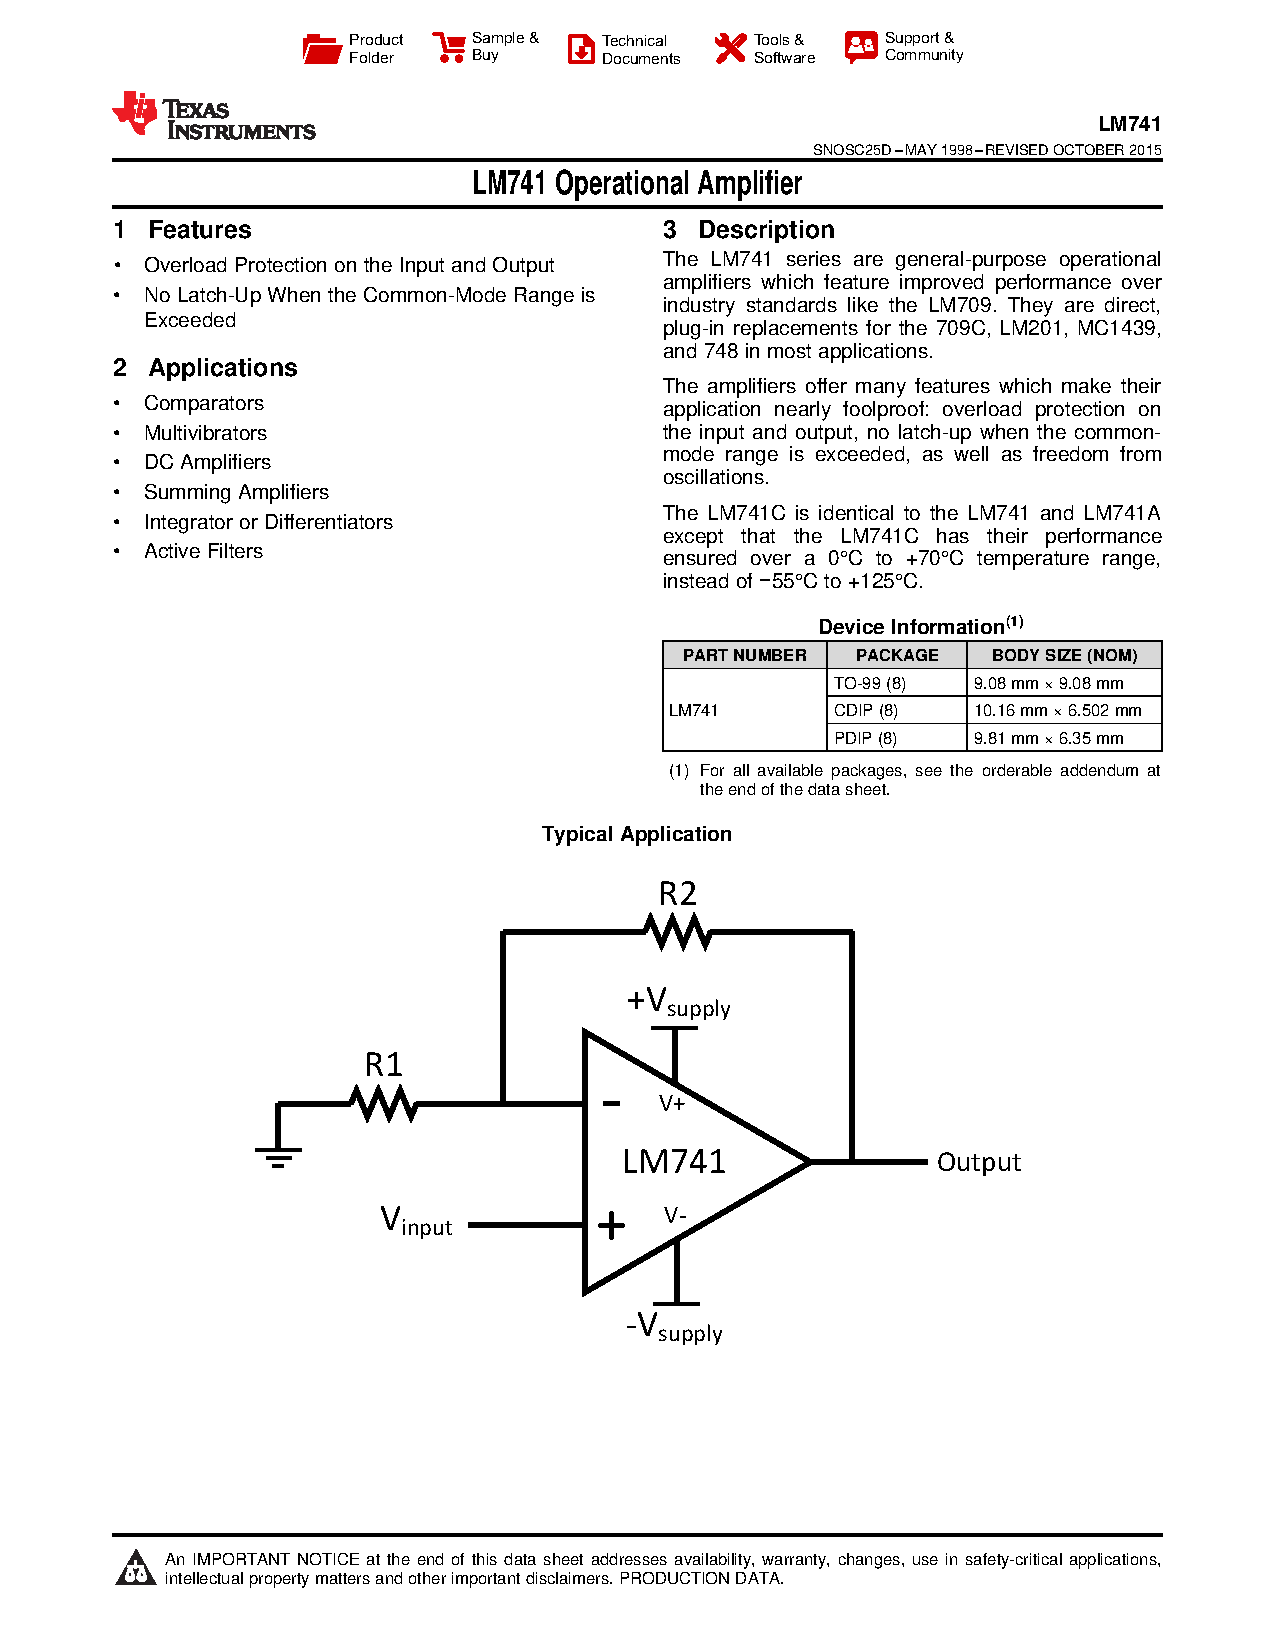
\includepdf[scale=0.7,pages=1,angle=0,pagecommand=\section{Amplificador Operacional 741}\label{hc:ao_741}]{HojasDeCaracteristicas/ejemplo_lm741.pdf}
% Resto de páginas
\includepdf[scale=0.7,pages=2-4,angle=0]{HojasDeCaracteristicas/ejemplo_lm741.pdf}


\end{document}
